%!TEX root = ../Thesis.tex

% This information is used in titlepage, colophon, preface and hyperref setup (pdf metainfo), and other options.

%\def\thesistypeabbr{B.Eng.}
%\def\thesistype    {Bachelor of Engineering}
%\def\thesistypeabbr{B.Sc.Eng.}
%\def\thesistype    {Bachelor of Science in Engineering}
\def\thesistypeabbr{M.Sc.}
\def\thesistype    {Master of Science in Engineering}
%\def\thesistypeabbr{Ph.D.}
%\def\thesistype    {Doctor of Philosophy}

\def\thesisauthor  {Thomas Nygaard Nilsson, s144470}
\def\thesistitle   {Master's Thesis}
\def\thesissubtitle{\emph{A Flutter Package for Real-Time Mobility Feature Computation}}
\def\thesislocation{Kongens Lyngby, Denmark}

\def\papersize    {b5paper} % Final papersize (b5paper/a4paper), recommended papersize for DTU Compute is b5paper
\def\showtrims    {false} % Print on larger paper than \papersize and show trim marks (true/false)?

\def\showtodos    {false}  % Show todos (true/false)?
\def\confidential {false} % Confidential thesis (true/false)?



%!TEX TS-program = xelatex
%!TEX root = ../Thesis.tex
\RequirePackage[l2tabu,orthodox]{nag} % Old habits die hard

\newcommand{\papersizeswitch}[3]{\ifnum\strcmp{\papersize}{#1}=0#2\else#3\fi}
\papersizeswitch{b5paper}{\def\classfontsize{10pt}}{\def\classfontsize{12pt}}

\documentclass[\classfontsize,\papersize,twoside,showtrims,extrafontsizes]{memoir}

% %!TEX root = ../Thesis.tex
% \RequirePackage[l2tabu,orthodox]{nag} % Old habits die hard

% \newcommand{\papersizeswitch}[3]{\ifnum\strcmp{\papersize}{#1}=0#2\else#3\fi}
% \papersizeswitch{b5paper}{\def\classfontsize{10pt}}{\def\classfontsize{12pt}}

% \documentclass[\classfontsize,\papersize,twoside,showtrims,extrafontsizes]{memoir}
\RequireXeTeX

\showtrimsoff
\papersizeswitch{b5paper}{
    % Stock and paper layout
    \pagebv
    \setlrmarginsandblock{26mm}{20mm}{*}
    \setulmarginsandblock{35mm}{30mm}{*}
    \setheadfoot{8mm}{10mm}
    \setlength{\headsep}{7mm}
    \setlength{\marginparwidth}{18mm}
    \setlength{\marginparsep}{2mm}
}{
    \papersizeswitch{a4paper}{
        \pageaiv
        \setlength{\trimtop}{0pt}
        \setlength{\trimedge}{\stockwidth}
        \addtolength{\trimedge}{-\paperwidth}
        \settypeblocksize{634pt}{448.13pt}{*}
        \setulmargins{4cm}{*}{*}
        \setlrmargins{*}{*}{0.66}
        \setmarginnotes{17pt}{51pt}{\onelineskip}
        \setheadfoot{\onelineskip}{2\onelineskip}
        \setheaderspaces{*}{2\onelineskip}{*}
    }{
    }
}
\ifnum\strcmp{\showtrims}{true}=0
    % For printing B5 on A4 with trimmarks
    \showtrimson
    \papersizeswitch{b5paper}{\stockaiv}{\stockaiii}
    \setlength{\trimtop}{\stockheight}
    \addtolength{\trimtop}{-\paperheight}
    \setlength{\trimtop}{0.5\trimtop}
    \setlength{\trimedge}{\stockwidth}
    \addtolength{\trimedge}{-\paperwidth}
    \setlength{\trimedge}{0.5\trimedge}
    
    % bigger todos if trim marks
    \setmarginnotes{10pt}{95pt}{\onelineskip}

    \trimLmarks
    
    % put jobname in left top trim mark
    \renewcommand*{\tmarktl}{%
      \begin{picture}(0,0)
        \unitlength 1mm
        \thinlines
        \put(-2,0){\line(-1,0){18}}
        \put(0,2){\line(0,1){18}}
        \put(3,15){\normalfont\ttfamily\fontsize{8bp}{10bp}\selectfont\jobname\ \
          \today\ \ 
          \printtime\ \ 
          Page \thepage}
      \end{picture}}

    % Remove middle trim marks for cleaner layout
    \renewcommand*{\tmarktm}{}
    \renewcommand*{\tmarkml}{}
    \renewcommand*{\tmarkmr}{}
    \renewcommand*{\tmarkbm}{}
\fi

\checkandfixthelayout                 % Check if errors in paper format!
\sideparmargin{outer}                 % Put sidemargins in outer position (why the fuck is this option not default by the class?)

% Large environments
\usepackage{microtype}
\usepackage{mathtools}
\usepackage{listings}                 % Source code printer for LaTeX
\usepackage{tikz}

% Links
\usepackage[hyphens]{url}             % Allow hyphens in URL's
\usepackage[unicode=false,psdextra]{hyperref}                 % References package

% Graphics and colors
\usepackage{graphicx}                 % Including graphics and using colours
\usepackage{xcolor}                   % Defined more color names
\usepackage{eso-pic}                  % Watermark and other bag
\usepackage{preamble/dtucolors}
\graphicspath{{graphics/}}

% Language
\usepackage{polyglossia}    % multilingual typesetting and appropriate hyphenation
\setdefaultlanguage{english}
\usepackage{csquotes}       % language sensitive quotation facilities

% Bibliography (references)
\usepackage[backend=biber,
            style=alphabetic,
            %backref=true,
            abbreviate=false,
            dateabbrev=false,
            alldates=long]{biblatex}

% Floating objets, captions and references
\usepackage{flafter}  % floats is positioned after or where it is defined! 
%\setfloatlocations{figure}{bhtp}   % Set floats for all figures
%\setfloatlocations{table}{bhtp}    % Set floats for all tables
%\setFloatBlockFor{section}         % Typeset floats before each section
\usepackage[noabbrev,nameinlink,capitalise]{cleveref} % Clever references. Options: "fig. !1!" --> "!Figure 1!"
\hangcaption
\captionnamefont{\bfseries}
\subcaptionlabelfont{\bfseries}
\newsubfloat{figure}
\newsubfloat{table}
%\letcountercounter{figure}{table}         % Consecutive table and figure numbering
%\letcountercounter{lstlisting}{table}     % Consecutive table and listings numbering
\captiontitlefinal{.}
% strip things from equation references, making them "(1)" instead of "Equation~1"
% from http://tex.stackexchange.com/questions/122174/how-to-strip-eq-from-cleveref
\crefformat{equation}{(#2#1#3)}
\crefrangeformat{equation}{(#3#1#4) to~(#5#2#6)}
\crefmultiformat{equation}{(#2#1#3)}%
{ and~(#2#1#3)}{, (#2#1#3)}{ and~(#2#1#3)}

% Table of contents (TOC)
\setcounter{tocdepth}{1}              % Depth of table of content
\setcounter{secnumdepth}{2}           % Depth of section numbering
\setcounter{maxsecnumdepth}{3}        % Max depth of section numbering

% Todos
\usepackage{totcount}                 % For total counting of counters
\def\todoshowing{}
\ifnum\strcmp{\showtodos}{false}=0
    \def\todoshowing{disable}
\fi
\usepackage[colorinlistoftodos,\todoshowing]{todonotes} % Todonotes package for nice todos
\newtotcounter{todocounter}           % Creates counter in todo
\let\oldtodo\todo
\newcommand*{\newtodo}[2][]{\stepcounter{todocounter}\oldtodo[#1]{\thesection~(\thetodocounter)~#2}}
\let\todo\newtodo
\let\oldmissingfigure\missingfigure
\newcommand*{\newmissingfigure}[2][]{\stepcounter{todocounter}\oldmissingfigure[#1]{\thesection~(\thetodocounter)~#2}}
\let\missingfigure\newmissingfigure
\makeatletter
\newcommand*{\mylistoftodos}{% Only show list if there are todos
\if@todonotes@disabled
\else
    \ifnum\totvalue{todocounter}>0
        \markboth{\@todonotes@todolistname}{\@todonotes@todolistname}
        \phantomsection\todototoc
        \listoftodos
    \else
    \fi
\fi
}
\makeatother
\newcommand{\lesstodo}[2][]{\todo[color=green!40,#1]{#2}}
\newcommand{\moretodo}[2][]{\todo[color=red!40,#1]{#2}}

% Chapterstyle
\makeatletter
\makechapterstyle{mychapterstyle}{
    \chapterstyle{default}
    \def\format{\normalfont\sffamily}

    \setlength\beforechapskip{0mm}

    \renewcommand*{\chapnamefont}{\format\HUGE}
    \renewcommand*{\chapnumfont}{\format\fontsize{30}{30}\selectfont}
    \renewcommand*{\chaptitlefont}{\format\fontsize{30}{30}\selectfont}

    \renewcommand*{\printchaptername}{\chapnamefont\MakeUppercase{\@chapapp}}
    \patchcommand{\printchaptername}{\begingroup\color{black}}{\endgroup}
    \renewcommand*{\chapternamenum}{\space\space}
    \patchcommand{\printchapternum}{\begingroup\color{dtured}}{\endgroup}
    \renewcommand*{\printchapternonum}{%
        \vphantom{\printchaptername\chapternamenum\chapnumfont 1}
        \afterchapternum
    }

    \setlength\midchapskip{1ex}

    \renewcommand*{\printchaptertitle}[1]{\raggedleft \chaptitlefont ##1}
    \renewcommand*{\afterchaptertitle}{\vskip0.5\onelineskip \hrule \vskip1.3\onelineskip}
}
\makeatother
\chapterstyle{mychapterstyle}

% Header and footer
\def\hffont{\sffamily\small}
\makepagestyle{myruled}
\makeheadrule{myruled}{\textwidth}{\normalrulethickness}
\makeevenhead{myruled}{\hffont\thepage}{}{\hffont\leftmark}
\makeoddhead{myruled}{\hffont\rightmark}{}{\hffont\thepage}
\makeevenfoot{myruled}{}{}{}
\makeoddfoot{myruled}{}{}{}
\makepsmarks{myruled}{
    \nouppercaseheads
    \createmark{chapter}{both}{shownumber}{}{\space}
    \createmark{section}{right}{shownumber}{}{\space}
    \createplainmark{toc}{both}{\contentsname}
    \createplainmark{lof}{both}{\listfigurename}
    \createplainmark{lot}{both}{\listtablename}
    \createplainmark{bib}{both}{\bibname}
    \createplainmark{index}{both}{\indexname}
    \createplainmark{glossary}{both}{\glossaryname}
}
\pagestyle{myruled}
\copypagestyle{cleared}{myruled}      % When \cleardoublepage, use myruled instead of empty
\makeevenhead{cleared}{\hffont\thepage}{}{} % Remove leftmark on cleared pages

\makeevenfoot{plain}{}{}{}            % No page number on plain even pages (chapter begin)
\makeoddfoot{plain}{}{}{}             % No page number on plain odd pages (chapter begin)

% \*section, \*paragraph font styles
\setsecheadstyle              {\huge\sffamily\raggedright}
\setsubsecheadstyle           {\LARGE\sffamily\raggedright}
\setsubsubsecheadstyle        {\Large\sffamily\raggedright}
%\setparaheadstyle             {\normalsize\sffamily\itseries\raggedright}
%\setsubparaheadstyle          {\normalsize\sffamily\raggedright}


% Hypersetup
\hypersetup{
    pdfauthor={\thesisauthor{}},
    pdftitle={\thesistitle{}},
    pdfsubject={\thesissubtitle{}},
    pdfdisplaydoctitle,
    bookmarksnumbered=true,
    bookmarksopen,
    breaklinks,
    linktoc=all,
    plainpages=false,
    unicode=true,
    colorlinks=false,
    citebordercolor=dtured,           % color of links to bibliography
    filebordercolor=dtured,           % color of file links
    linkbordercolor=dtured,           % color of internal links (change box color with linkbordercolor)
    urlbordercolor=s13,               % color of external links
    hidelinks,                        % Do not show boxes or colored links.
}
% Hack to make right pdfbookmark link. The normal behavior links just below the chapter title. This hack put the link just above the chapter like any other normal use of \chapter.
% Another solution can be found in http://tex.stackexchange.com/questions/59359/certain-hyperlinks-memoirhyperref-placed-too-low
\makeatletter
\renewcommand{\@memb@bchap}{%
  \ifnobibintoc\else
    \phantomsection
    \addcontentsline{toc}{chapter}{\bibname}%
  \fi
  \chapter*{\bibname}%
  \bibmark
  \prebibhook
}
\let\oldtableofcontents\tableofcontents
\newcommand{\newtableofcontents}{
    \@ifstar{\oldtableofcontents*}{
        \phantomsection\addcontentsline{toc}{chapter}{\contentsname}\oldtableofcontents*}}
\let\tableofcontents\newtableofcontents
\makeatother

% Confidential
\newcommand{\confidentialbox}[1]{
    \put(0,0){\parbox[b][\paperheight]{\paperwidth}{
        \begin{vplace}
            \centering
            \scalebox{1.3}{
                \begin{tikzpicture}
                    \node[very thick,draw=red!#1,color=red!#1,
                          rounded corners=2pt,inner sep=8pt,rotate=-20]
                          {\sffamily \HUGE \MakeUppercase{Confidential}};
                \end{tikzpicture}
            }
        \end{vplace}
    }}
}

% Prefrontmatter
\newcommand{\prefrontmatter}{
    \pagenumbering{alph}
    \ifnum\strcmp{\confidential}{true}=0
        \AddToShipoutPictureBG{\confidentialbox{10}}   % 10% classified box in background on each page
        \AddToShipoutPictureFG*{\confidentialbox{100}} % 100% classified box in foreground on first page
    \fi
}

% DTU frieze
\newcommand{\frieze}{%
    \AddToShipoutPicture*{
        \put(0,0){
            \parbox[b][\paperheight]{\paperwidth}{%
                
\includegraphics[trim=130mm 0 0 0,width=0.9\textwidth]{DTU-frise-SH-15}
                \vspace*{2.5cm}
            }
        }
    }
}

% This is a double sided book. If there is a last empty page lets use it for some fun e.g. the frieze.
% NB: For a fully functional hack the \clearpage used in \include does some odd thinks with the sequence numbering. Thefore use \input instead of \include at the end of the book. If bibliography is used at last everything should be ok.
\makeatletter
% Adjust so gatherings is allowd for single sheets too! (hacking functions in memoir.dtx)
\patchcmd{\leavespergathering}{\ifnum\@memcnta<\tw@}{\ifnum\@memcnta<\@ne}{
    \leavespergathering{1}
    % Insert the frieze
    \patchcmd{\@memensuresigpages}{\repeat}{\repeat\frieze}{}{}
}{}
\makeatother


% BELOW IS BY THOMAS
%\usepackage{preamble/custom_packages/pythonhighlight}
% https://github.com/olivierverdier/python-latex-highlighting
\usepackage{algorithm}
\usepackage[final]{pdfpages}
\usepackage{amsfonts} % math

\usepackage[ruled,vlined]{algorithm2e}
\renewcommand{\algorithmicrequire}{\textbf{Input:}}
\renewcommand{\algorithmicensure}{\textbf{Output:}}
%!TEX root = ../Thesis.tex

% Text fonts (http://www.macfreek.nl/memory/Fonts_in_LaTeX)
% Install fonts from /usr/local/texlive/<version>/texmf-dist/fonts/opentype/public
\usepackage{fontspec}

% Sans-serif font
% \setsansfont[
%     Ligatures=TeX,
%     Extension=.otf,
%     UprightFont=*-regular,
%     BoldFont=*-bold,
%     ItalicFont=*-italic,
%     BoldItalicFont=*-bolditalic,
%     %SlantedFont=,
%     %BoldSlantedFont=,
%     %SmallCapsFont=
%     Scale=0.8      % Adjustmens when using math in sections
% ]{texgyreadventor}
% \setsansfont[Ligatures=TeX]{Neo Sans Intel}    % Neo Sans Intel – Like DTU font but more symbols
% \setsansfont[
%     Ligatures=TeX,
%     Scale=0.8
% ]{NeoSans}           % NeoSans – DTU font (missing `+' symbols and other)
% \setsansfont[Ligatures=TeX]{CMU Sans Serif}    % Computer Modern Unicode font
\setsansfont[Ligatures=TeX]{Latin Modern Sans} % Latin Modern Sans serif font

% %Use this for more convienent sans serif font in math mode.
% \setmathsf{Latin Modern Sans}


%!TEX root = ../Thesis.tex

% Content specific packages.

\usepackage{blindtext}
\usepackage{algorithm}
\usepackage{algpseudocode}
%\usepackage{pgfplots}                 % Plot tools
%\usetikzlibrary{
%    arrows,
%    matrix,
%    positioning,
%    shapes,
%    topaths,
%}
%\pgfplotsset{compat=1.7}

% Listings
\lstset{
    basicstyle=\footnotesize\ttfamily,% the size of the fonts that are used for the code
    breakatwhitespace=false,          % sets if automatic breaks should only happen at whitespace
    breaklines=true,                  % sets automatic line breaking
    captionpos=b,                     % sets the caption-position to bottom
    commentstyle=\color{s14a},        % comment style
    deletekeywords={},                % if you want to delete keywords from the given language
    escapeinside={\%*}{*)},           % if you want to add LaTeX within your code
    frame=single,                     % adds a frame around the code
    keywordstyle=\bfseries\ttfamily\color{s09}, % keyword style
    language=Python,                  % the language of the code
    morekeywords={*,...},             % if you want to add more keywords to the set
    numbers=left,                     % where to put the line-numbers; possible values are (none, left, right)
    numbersep=5pt,                    % how far the line-numbers are from the code
    numberstyle=\sffamily\tiny\color{dtugray}, % the style that is used for the line-numbers
    rulecolor=\color{dtugray},        % if not set, the frame-color may be changed on line-breaks within not-black text (e.g. comments (green here))
    showspaces=false,                 % show spaces everywhere adding particular underscores; it overrides 'showstringspaces'
    showstringspaces=false,           % underline spaces within strings only
    showtabs=false,                   % show tabs within strings adding particular underscores
    stepnumber=1,                     % the step between two line-numbers. If it's 1, each line will be numbered
    stringstyle=\color{s07},          % string literal style
    tabsize=2,                        % sets default tabsize to 2 spaces
    title=\lstname,                   % show the filename of files included with \lstinputlisting; also try caption instead of title
}

\usepackage{pdflscape}
\usepackage{acronym}
\usepackage{enumitem}


\usepackage{color}
\definecolor{purple}{RGB}{160,32,240}
\definecolor{blue}{RGB}{0,0,255}
\definecolor{orange}{rgb}{1,0.5,0}
\definecolor{green}{rgb}{0,100,0}

%\newcommand{\todo}[1]{\textsf{\textcolor{orange}{[#1]}}}
\newcommand{\note}[1]{{\textcolor{blue}{[#1]}}}

% THOMAS BELOW
\usepackage{minted} % python code

\addbibresource{bibliography/Bibliography.bib}
% SET NO INDENT
\setlength{\parindent}{0pt}
\begin{document}

\prefrontmatter
%!TEX root = ../Thesis.tex 
\thispagestyle{empty}             % No page numbers
\calccentering{\unitlength}
\begin{adjustwidth*}{\unitlength}{-\unitlength}
    \begin{adjustwidth}{-0.5cm}{-0.5cm}
        \sffamily
        \begin{flushright}
            \thesistypeabbr{} Thesis\\*[0cm]
            \thesistype{}\\
        \end{flushright}
        \vspace*{\fill}
        \noindent
        
\includegraphics[width=0.75\textwidth]{DTU-Compute-B-UK}\\*[0.5cm]
        \HUGE \thesistitle{}\\*[0.2cm]
        \Huge \thesissubtitle{}\\*[1.2cm]
        \parbox[b]{0.5\linewidth}{%
            \LARGE 
            \thesisauthor{}\\*[1.2cm]
            \Large
            \thesislocation{} \the\year
        }
        \hfill
\includegraphics[scale=0.7]{DTU-logo-CMYK}
    \end{adjustwidth}
\end{adjustwidth*}
\normalfont
\normalsize

\cleartoevenpage
%!TEX root = ../Thesis.tex
\thispagestyle{empty} % No page numbers
\frieze
\vspace*{\fill}
\noindent
\sffamily
\small
\textbf{DTU Compute}\\
\textbf{Department of Applied Mathematics and Computer Science}\\
\textbf{Technical University of Denmark}\\
\\
Matematiktorvet\\
Building 303B\\
2800 Kongens Lyngby, Denmark\\
Phone +45 4525 3031\\
compute@compute.dtu.dk\\
www.compute.dtu.dk\\
\normalsize
\normalfont
\vspace*{2.5cm}

\clearforchapter

\frontmatter
%!TEX root = ../Thesis.tex
\chapter{Summary}
This is an example and template for a \acf{PDR} to be used when initiating a Thesis.

\noindent
\note{Text written like this are generic notes and guidelines.}

%!TEX root = ../Thesis.tex
\chapter{Preface}
This Master's thesis was prepared at the department of \textit{Applied Mathematics and Computer Science} at the Technical University of Denmark in fulfillment of the requirements for acquiring a MSc degree in \textit{Human-Centered Artificial Intelligence}.

\vfill

{
\centering
    \thesislocation{}, \today\\[1cm]
    \hspace{3cm}
\includegraphics[scale=0.4]{graphics/signature.png}\\[1cm]
\begin{flushright}
    \thesisauthor{}
\end{flushright}
}
%!TEX root = ../Thesis.tex
\chapter{Acknowledgements}
Lorem ipsum dolor sit amet, consectetur adipisicing elit, sed do eiusmod tempor incididunt ut labore et dolore magna aliqua. Ut enim ad minim veniam, quis nostrud exercitation ullamco laboris nisi ut aliquip ex ea commodo consequat. Duis aute irure dolor in reprehenderit in voluptate velit esse cillum dolore eu fugiat nulla pariatur. Excepteur sint occaecat cupidatat non proident, sunt in culpa qui officia deserunt mollit anim id est laborum.

\clearforchapter
\tableofcontents
\clearforchapter
\mylistoftodos

\mainmatter
\chapter{Introduction}
This chapter will provide an introduction to the thesis by laying out the motivation and background as well as the problem statement and the goals which were set out to be achieved.\\

All source code used in this thesis can be found at \url{https://github.com/thomasnilsson/mobility-features-thesis}.

\section{Context and Motivation}
% Almost every Chapter 1 begins with a section that sets the scene and that motivates the problem being studied. It describes some domain and indicates a problem in general terms.

% Some questions you should be able to answer after reading the motivation section are:

% What is the general area being addressed?
Most people walk around with a very powerful computer in their pocket, that contains a variety of sensors capable of painting a picture of the user's current context. A user's context is a set of digital characteristics, also called features, which arise from an individual interacting with their environment, such as when moving around between places in one's everyday life. This thesis will describe the design and implementation of a software package for the Flutter framework capable of generating a fully-automated mobility context in real-time, by tracking location data on a smart-phone. The package will in the future integrate into the CARP Mobile Sensing Framework (CAMS)\footnote{\url{https://github.com/cph-cachet/carp.sensing-flutter/wiki}} which provides an array of digital phenotyping capabilities to an application developer.\\

\subsection*{Challenges in Mobile Computing Research}
% Is it a 'theoretical' problem that is worth solving?
The research problem addressed in this project is focused on the software engineering aspect of developing a digital phenotyping library and relates to the \textit{re-usability of source code} as well as the current \textit{lack of support for real-time computation}.

\subsubsection*{Re-usability of Source Code}
There have been numerous contributions within the field of using smartphone data for phenotyping and predicting the user's state for many years. However, much of the research conducted, specifically within the field of user-mobility context generation, has been done without publishing source code in a way such that it may be used by other researchers in the future. Mainly this comes down to researchers not publishing the source code at all, due to source code not being the focus of their research. Sometimes the source code is released, however, but then over time suffers from an (understandable) lack of maintenance and thus becomes obsolete. Furthermore, researchers tend to focus on only the Android platform since this is the more prevalent platform of choice in many countries, however, this is not a good research practice for reasons we will elaborate on later.

\subsubsection*{Lack of Support for Real-time Computation}
In addition, the existing contributions gather all of the data before feature computation is carried out. This has the clear advantage of making it easier to run and evaluate the mobility feature algorithms. However, this also has the disadvantage that the feature generation is not possible in real-time, where they are the most useful. Certain features rely on prior contexts being computed and readily available and are therefore easily implemented when done in an off-line fashion on a desktop computer. However, in a real-time situation on a phone, these prior contexts will need to be stored on a device that has limited storage, and the algorithms must be adjusted to read in these stored set contexts. The proposed software package will solve the problem of implementing these algorithms from scratch as well as allow the application programmer to compute the user's mobility context in real-time.

\subsection*{Who Would Benefit from This?}
% Would anyone care if I solved this?
Researchers within the field of mental health illnesses from a health-tech background will benefit greatly from using a Flutter package with a high level of abstraction, in which the researcher's focus is moved from software engineering to data analysis and study design. Currently, researchers often choose to start from scratch which is a laborious task that takes up valuable time which could be spent on more relevant work. Furthermore, since Flutter is capable of compiling to both iOS and Android source code, studies need not be restricted to a single mobile platform, hence why Flutter was the app-framework of choice.\\

An additional benefit of computing features on the phone itself, in contrast to computing it on a central server or desktop, is the anonymization of GPS data; the generated context contains information that is much less sensitive and therefore has implications on privacy as well as GDPR compliance.



\section{Background}
% Some authors provide a miniature literature review to give the reader enough background to understand the context of the research; a full review is usually deferred to the second chapter of the thesis. Other authors do the full review in Chapter 1, but that is rarer.

% Some questions you should be able to answer in general terms after reading this section are:
% This section will provide a context for the thesis in the form of a short introduction to the topic of depression and secondly a brief literature review within mobile sensing and its applications.

% Depression and treatments
Major Depressive Disorder (MDD), commonly known as depression, is a serious illness that is currently treated with medication or through therapy. Dobson et al. \cite{randomized_trial_behavioural_activation} discusses how medication is the current treatment standard for severe cases of depression, with cognitive therapy, a form of psychotherapy, being the most widely investigated treatment for more moderate cases. Traditional psychotherapy is resource-intensive since it relies on traditional methods that involve face-to-face consultations. Chartier and Provencher \cite{behavioural_activation_for_depression} describe the need to identify effective, evidence-based treatments that are time and cost-effective to increase the population's accessibility to treatments. The treatment form of \textit{behavioral activation}, a component of cognitive-behavioral therapy, is receiving increased attention and empirical support as a stand-alone psychotherapy method for treating depression. Dobson et al. found that behavioral activation performed similarly to antidepressant medication. Furthermore, the findings were also that behavioral activation is less expensive and longer-lasting alternatives to medication in the treatment of depression.  \\

% Mobile sensing
Mobile sensing involves the use of the phone's sensors to collect objective user data and may include predicting the user state from this data. The objectivity of the data stems from the data being collected from sensors in contrast to subjective user data such as questionnaires. Mobile sensing has become especially prevalent in the last few years due to the rise of ubiquitous computing. Applications of mobile sensing include mental health monitoring also known as \textit{digital phenotyping} or \textit{user context generation}. Within mental healthcare, mHealth opens the potential for practical and low-cost solutions for psychological interventions \cite{mobile-based-interventions}. MHealth also enables mental healthcare to reach populations that do not have access to traditional psychotherapy \cite{future-mental-health}, such as developing countries. Gravenhorst et al. \cite{Gravenhorst2015} describes how mobile phones, in particular in the area of mental disorders, can result in a better treatment that can reach more users, at a lower cost compared to traditional methods.\\ 

Within the context of mHealth for behavior and mental state, location data is commonly used. Rohani et al. \cite{rohani2018-correlations} found in a review of 46 studies that several of them showed consistent and statistically significant correlations between objective behavioral features collected via mobile and wearable devices and depressive mood symptoms. In addition, they conclude that continuous- and everyday monitoring of behavioral metrics could be a promising supplementary objective measure for estimating depressive mood symptoms. As behavioral activation requires an understanding of the user's mental state and behavior it is an ideal application for using objective mobility features. \\



\section{Research Question}
% This section provides a very concise statement of your hypothesis/thesis/problems. The hypothesis or thesis is the highest-level problem or goal you are going to address. The specific list of problems --- usually a handful, although sub-problems are sometimes given --- are things that need to be solved if you are going to satisfy your hypothesis/thesis. Problems should be stated unambiguously. The importance of the problem should be mentioned if it hasn't already been done so in the prior sections. Of course, the problem must be worthy of a thesis.

Existing contributions within the field of generating mobility features and context are cumbersome, if even possible, to reproduce with regards to their source code. Furthermore, the algorithms that exist in the literature do not necessarily lend themselves to the real-time computation of features. How these two things can be achieved will be investigated in this thesis and are addressed in the following research questions:\\

\textbf{Question 1:} \textit{Which mobility features are relevant to include in a software package?}\\

\textbf{Question 2:} \textit{How can these features be computed in real-time, on a smartphone device?}\\

\textbf{Question 3:} \textit{How does the API design of such a software package look like?}\\

\section{Goals and Methods}
% While the above section details the problems, your job is to then translate those problems into research goals. Each goal should briefly indicate how you are going to solve the problem i.e., the method you will use to solve it. Note that some authors sometimes combine problem statements/goals/methods into a single section, while others separate it. Goals should be operational, i.e., if you later claim to achieve your goal, you should be able to match your solution against the goal statement.

% I cannot overstate how important it is to have clear goals. Most examiners highlight these goals, and after reading the thesis they then go back to see if you have actually accomplished your goals. If you have not, then you have a big problem with your thesis. Even worse are theses where problems and goals are not clearly stated, for it means people are trying to evaluate your solutions in a vacuum.

The research goals closely match the research questions and will explain how the different sub-questions are answered, and which methods are used to do so.

\subsubsection*{Goal 1: Implement the Off-line Mobility Feature Algorithms}
Saeb et al. \cite{Saeb2015} describes a list of mobility features, some of which they prove to strongly correlate with depressive behavior. These features need to be implemented in their most simple form, i.e. off-line, where all the location data for a given day is readily available. This will be carried out in Python with a synthetic dataset and later in Dart. This is done in order to demonstrate the quality of the algorithms. A pre-processing procedure inspired by Cuttone et al. \cite{sparse-location-2014} for finding certain features has been implemented by Jonas Busk prior to starting this thesis. 

\subsubsection*{Goal 2: Adapt Algorithms to Work in Real-time}
The features described above will be implemented such that they can be evaluated on a partial dataset, i.e. an incomplete day's data. Many of the features will have minor changes applied to their calculation, however, the \textit{Routine Index} feature as defined by Canzian et al.\cite{Canzian2015} and Saeb et al. \cite{Saeb2015} may prove to be a challenge to implement in real-time. By its definition, this feature lends itself to be computed only once multiple full days of data have been collected, making the feature non-trivial to implement in a real-time fashion where it may compute on a partial, incomplete dataset. 

\subsubsection*{Goal 3: Implement Real-time Mobility Features in Flutter}
An algorithm/procedure that runs the Mobility Feature algorithms on a smart-phone has to be written which involves a couple of steps. Location data has to be collected and stored on the smartphone, and then it has to be demonstrated that features can be computed whenever they need to be. However, storing raw data every day would end up taking up too much disk space and is therefore not an ideal solution when working with a smartphone. This means the solution has to be able to compute these history-dependent features without relying on storing raw data of each day.

\subsubsection*{Goal 4: Design a Flutter Software Package}
The software package should be designed according to the Flutter packages best practices \footnote{\url{flutter.dev/docs/development/packages-and-plugins/developing-packages}}, be properly documented and be released on the Dart package manager \footnote{\url{www.pub.dev}}.

\subsubsection*{Goal 5: Develop a Demo Mobile Application}
To demonstrate how the software package containing the algorithm will be used in practice, a Flutter demo-app will be developed in parallel with the software package. The functionality of the application should be in accordance with the contents of \textit{Goal 3}. By developing an actual application and seeing the algorithms in use, the structure of the API should emerge such that it is 'nice to use' from an application developer's point of view.

\subsubsection*{Goal 6: Conduct a Field Study}
To test the quality of the Mobility Features in action, a small scale study of 5-10 participants should be conducted and should run for 2-4 weeks (the longer the better). The participants will use the demo application. Also, in order to validate the quality of the features produced daily during these weeks, the participants will have to fill out a small diary in order to compare the results of the algorithms with the subjective experience of the users. This diary will be a part of the demo application. Preferably the users should be reminded daily to fill out the diary such that as much user data is collected as possible.


\section{Results}
% Some theses, particularly PhDs, contain a section that summarizes the most important findings and casts these as contributions to the research field. These usually match the goals. They also include a short description as to why these findings are valuable.

In this section, it will be addressed to which extent the research questions and goals were met.

\subsubsection*{Which mobility features are relevant to include in a software package?}
The features described in \cite{Saeb2015} and \cite{extraction-of-behavioural-features} were implemented in Dart by using standard imperative language features such as loops and if-else clauses. Specifically, a set of intermediate features, namely\textit{ Stops}, \textit{Places}, and \textit{Moves}, were also implemented which aided in reducing the sheer amount of data processed by the feature-extraction algorithms. 

The most important features pertaining to depression were \textit{Home Stay}, \textit{Entropy/Normalized Entropy}, and the \textit{Routine Index}. All features except for the \textit{Routine Index} can be evaluated on a daily basis without the need for historical data, and as such those features were implemented first and the \textit{Routine Index} was implemented later. In addition to the features described by \cite{Saeb2015}, most of which are evaluated daily, the features were also extended to aggregate features which are a daily feature averaged over a period of the last 28 days. The \textit{Routine Index} features was chosen to be put in Among these aggregated features.

\subsubsection*{How can these features be computed in real-time, on a smartphone device?}
The Routine Index as well as the aggregate features, are calculated by storing the previously mentioned intermediate feature \textit{Stops} on the device. These features effectively serve as a compressed form of the raw dataset, which is saved on the device. The compressed dataset takes up three orders of magnitude less disk space compared to the corresponding raw data, which also made it possible to calculate those features which relied on historical data.

\subsubsection*{How does the API design of such a software package look like?}
All the implementation details of the algorithms were hidden away from the programmer and a high abstraction level API was provided, with thorough documentation on its usage. Even the problem of saving intermediate features on the device, such that they may be used in the future, was handled with minimal need for the programmer to be involved. In the process of developing this app, the quality of the \textit{Mobility Features Package}  was also improved both in the accuracy of the features but also in terms of the abstraction level of the API. However, a few abstraction-level decisions are still up for debate with regards to how \textit{open} the API should be, and whether or not the intermediate features should be part of it since they themselves contain sensitive information.

\subsubsection*{Field Study}
A field study with 10 participants was conducted in which a study app was developed in Flutter, in order to test the usage of the package. Due to Google restricting the Location API on Android shortly after the thesis plan was laid out, the study was conducted using only iPhones. This was done in order to not spend too much time on things out of our control. During the development of the application, the COVID-19 pandemic hit Europe, and therefore it was not possible to meet up with most of the participants physically. The demo application, therefore, had to be distributed digitally which was done via Apple's Testflight service, which is a good idea in any case, since it allows for quick patching of bug-fixes with minimal installation trouble to the users.
\section{Thesis Overview}

The process of developing the Mobility Features Package is documented in the following chapters for which a brief overview is given below.\\

\textbf{Chapter 2: Related Work} will outline a set of relevant contributions related to behaviour and mental state tracking through mobile sensing. \\

\textbf{Chapter 3: Theoretical Background} will describe all the theory behind computing the features. This includes definitions and discussion of all the features, as well as the algorithms that can extract mobility patterns from this data. The section is very mathematical as well as philosophical and lays the ground work for the later implementation.\\

\textbf{Chapter 4: Software Design} will discuss the design choices and principles used to model a software system capable of computing the mobility features. Design pertains to both how the internal system of the package works as well as the public facing API which is the interface the application programmer talks to when using the package.\\

\textbf{Chapter 5: Flutter Implementation} will describe how the domain model and the feature algorithms were implemented in the Dart language. How a user may use the final version of the package is also described.\\

\textbf{Chapter 6: Validation} will outline the field study that was conducted in which 10 participants. The participants were tracked with a mobile application that used the Mobility Features Package to compute daily features based on their location data. Implementation of the mobile application is also discussed in this chapter.\\

\textbf{Chapter 7: Results and Discussion} will include a data analysis of the study conducted in which the computed features are compared with the subjective answers given by participants. Additionally, further work is discussed which includes improvements to the package, the algorithms and concrete applications for the Mobility Features Package in the near future.\\

\textbf{Chapter 8: Conclusion} will report the major findings of the thesis and answer the research questions in detail.\\

\chapter{Related Work}
\label{chapter:02}
This chapter will describe what work has been done within the treatment of depression related to digital phenotyping and context generation. Secondly, a series of previous contributions will be presented which deal with computing mobility features including how these features can be used in a medical context. Thirdly, a brief insight into existing mobile sensing frameworks will be given, including how the \textit{Mobility Features Package} will fit into one of these frameworks. Lastly, an example of a recommender system is given for which the \textit{Mobility Features Package} is an ideal use case.

\section{Digital phenotyping: a global tool for psychiatry}
The paper \cite{digital_phenotyping} deals with the topic of collecting and aggregating user data into a so-called digital phenotype. It is predicted that by 2050, the biggest impact in psychiatry and mental health will have been the revolution in technology- and information science. Smartphones have become ubiquitous in the past decade and there are over three billion smartphones with a data plan worldwide, each of which has computing power which surpasses supercomputers of the 1990s. In areas around the world without easy access to clean water, ownership of a smartphone and by proxy, rapid access to information has become a symbol of modernity. 

\subsection{Phenotyping and Psychiatry}
In the realm of psychiatry, a current data collection problem is the dependence on self-reporting of sleep, appetite, and emotional state, even though it is recognized that depression will impair people's ability to remain objective in assessing their own behavior and thus data is prone to be faulty \cite{digital_phenotyping}. Another current problem is how it how people suffering from mental illness tend to not seek help before it is too late. Depressive relapses are therefore also often reported with considerable delay for patients currently in treatment. 

The smartphone offers an objective form of mental-state measurement which is referred to was \textit{Digital Phenotyping}, which uses built-in sensors such as geo-location, accelerometer, and human-computer interactions (HCI) to infer the state of the patient. This makes it possible to assess people by using data in a real-time fashion, rather than in retrospect as is currently is done. Digital phenotyping could in theory fill the role of a smoke detector which provides early signs of relapse and recovery, without replacing the face-to-face consultations entirely. In addition, this also allows researchers to track patients in their own environment, rather than in a clinical environment.

\subsection{The Ethical Dimension}
However, when does measurement become surveillance? Is phenotyping by using data such as geo-location too invasive? A series of ethical issues have to be addressed before digital phenotyping can realistically hope to be employed as a tool for population health. Although, some of these issues have technical solutions, such as with tracking human-computer-interactions which is mostly related to \textit{how} the user interacts with a device, i.e. the pacing with which is typed, scrolled or how long phone calls last - rather than the content of what is provided to the device i.e. what is typed, spoken during a phone call, or the websites visited. 

\section{Learning Significant Locations and Predicting User Movement With GPS}
This thesis by \cite{learning_significant_locations} from 2002 is one of the earliest contributions to present a system that uses GPS data to infer user context and use this context. 

\subsection{Data Collection}
For data collection, a wearable GPS receiver was used which tracked user location for four months with an accuracy of 15 meters, meaning the same physical location may have resulted in slightly different GPS coordinates from day today. For pre-processing data some of the data was discarded by setting the sensor to only log data while the user was traveling at a speed greater than 1 mile per hour, with the average human having a walking speed of about 3 miles per hour. 

\subsection{Finding Locations}
Given a data set of GPS points, a \textit{significant place} is found by examining data and finding periods of low user-movement. The duration of the period was (somewhat arbitrarily) chosen to be 10 minutes. Due to the 15 meter accuracy of the sensor, the location coordinates found may be somewhat noisy from day today. In order to identify the mean of these noisy place locations, a modified version of the \textit{K-means} clustering algorithm was applied to the dataset, with a radius parameter. The optimal radius for the clustering algorithm is found by examining the graph of the number of clusters found (K) as a function of the radius. The knee of the graph (see figure \ref{fig:knee-graph}) signifies the radius just before the number of locations begins to converge to the number of clusters found. This procedure effectively figures out which significant places belong to the same \textit{location} and which are outliers points which should be considered noise, i.e. they either do not belong to a location or there is too low confidence to say whether they do or not. 

\begin{figure}
    \centering
    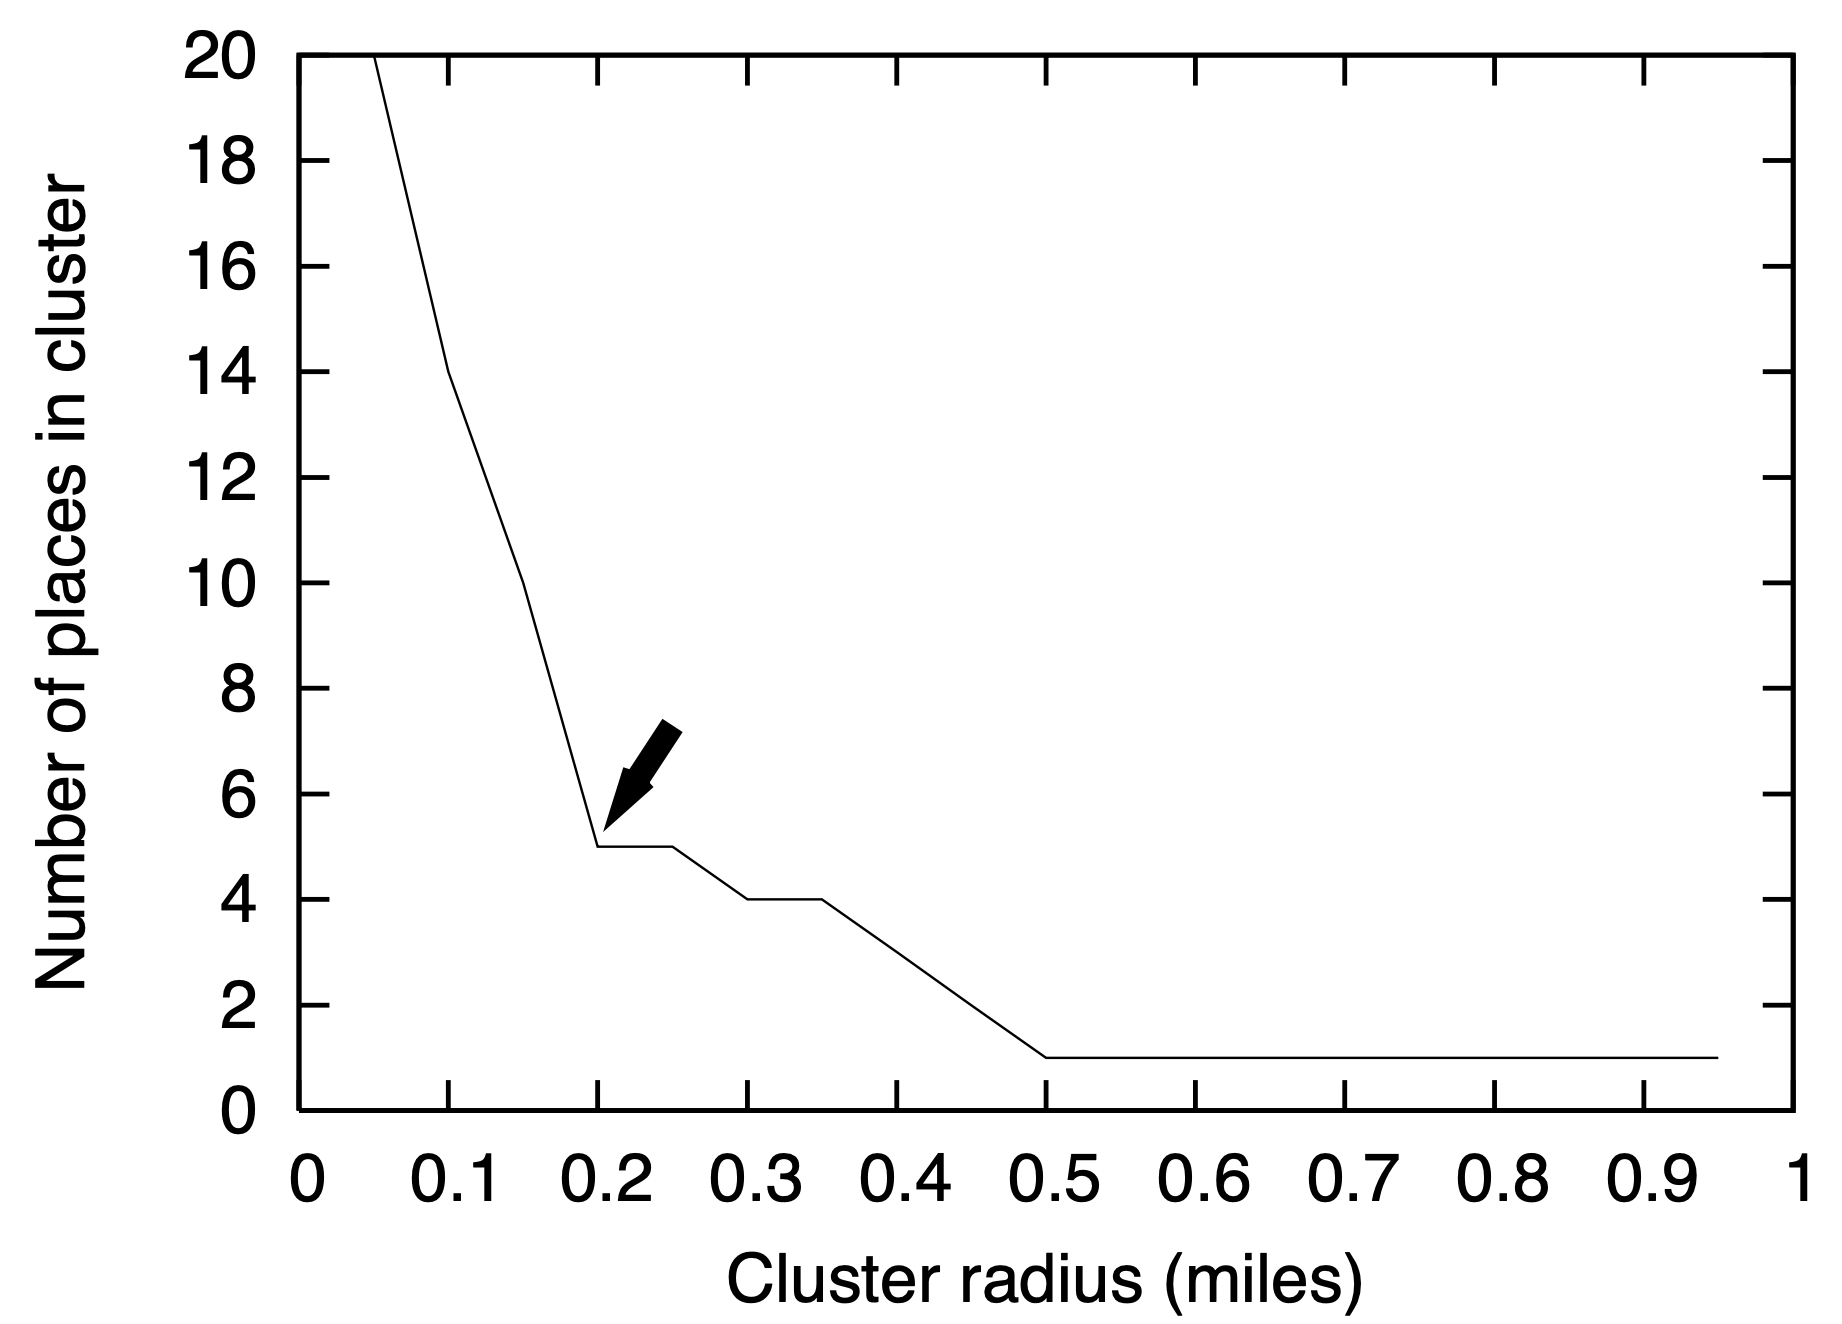
\includegraphics[width=0.5\textwidth]{images/knee_graph.png}
    \caption{The number of places found in the dataset the location radius parameter changes. The arrow indicates the knee in the graph at which point the radius will be used to find \textit{sub-locations}. Source \cite{learning_significant_locations}}
    \label{fig:my_label}
\end{figure}

\subsection{Finding Sub-locations}
Within a location, several \textit{sub-locations} may exist, which are perhaps best exemplified by a university campus, as a location, having several buildings for different departments, i.e. \textit{sub-locations}. To find these, all \textit{significant place} data-points belonging to a \textit{location} is given as input to previously described clustering algorithm. The optimal radius is once again found by looking at the knee on the graph and from this optimal parameter choice, the \textit{sub-locations} within a given location are identified.

\subsection{Prediction}
A Markov model was set up with each state representing a Location and transitions representing real-life transitions between locations. To compute the probability of a path, or a transition between places, the relative frequency of the path was computed.


\section{Density-based Spatial Clustering of Applications with Noise (DBSCAN)}
The DBSCAN algorithm is an essential algorithm for clustering GPS data points and was published by Martin Ester, Hans-Peter Kriegel, Jörg Sander, and Xiaowei Xu in 1996 \cite{density-based-1996}. The core concept of DBSCAN is to cluster location data based on a density measure rather than a pure distance measure, such as is the case with the \textit{K-means} clustering algorithm. This allows the clusters to take on nearly any shapes and sizes, in contrast to round shapes which are found by using \textit{K-means} and \textit{Gaussian Mixture Model}, see figure \ref{fig:dbscan_shapes} for examples.

\begin{figure}
    \centering
    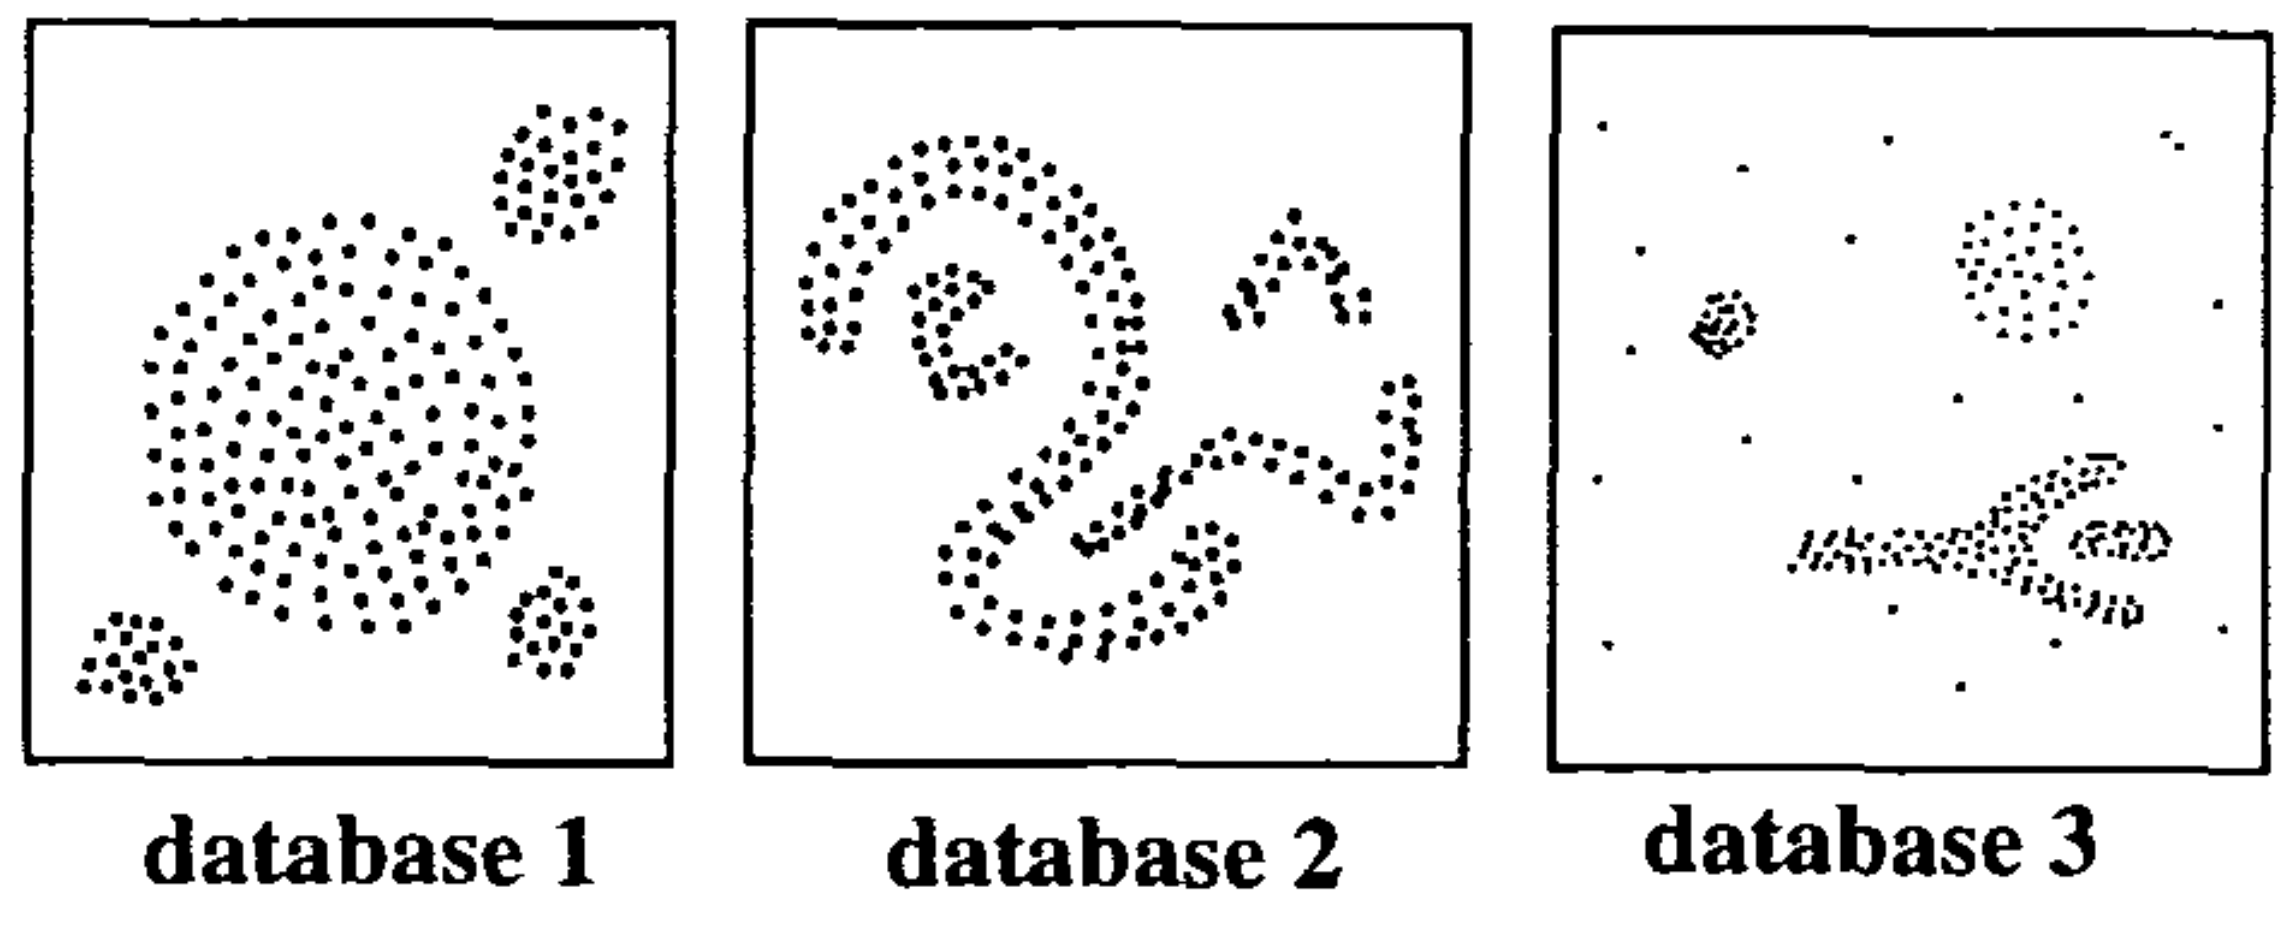
\includegraphics[width=\textwidth]{images/dbscan-clusters.png}
    \caption{Data from three different databases with very distinct cluster shapes. Database \#1 has very round clusters which would identified correctly with K-means whereas database \#2 and \#3 have clusters which would require a different clustering approach. Source: \cite{density-based-1996}}
    \label{fig:dbscan_shapes}
\end{figure}

GPS data has a higher density inside clusters than outside the clusters and the density in noisy areas is lower than density in clusters. Here, \textit{noisy} refers to points that are spread randomly within some areas and do not cluster around a centroid.

The DBSCAN algorithm will, given a set of geospatial data points and a small set of parameters, find these dense clusters, as well as noisy data points, where the clusters correspond to places and the noisy data points, are outliers which do not belong to a place. The output of the algorithm is labeling of each point in the input dataset as either belonging to a cluster or being a noisy data point.

\section{Mathematical Definitions}

The DBSCAN paper defines a \textit{Neighbourhood} as a collection of data points within some radius, i.e. an area defined by a distance function. Within a \textit{Neighbourhood}, two types of points can reside: \textit{Core points}, that is, points which are inside in the neighborhood, and \textit{Border points } which lie on the edge of the neighborhood and delimit it. 

\subsubsection*{Definition 1: Epsilon Neighbourhood}
An \textit{Epsilon Neighbourhood} is a \textit{Neighborhood} defined on a point $p$ which includes all the points $q$ which are inside a radius of $\epsilon$ of $p$. Formally this is defined as:\\

$$N_{\epsilon} (p) = q \in D \quad|\quad dist(p,q) \leq \epsilon$$

\textit{Note: The $N_{\epsilon}$ of a border point contains much fewer points than that of a core point. }\\

We Require for all points $p$ and a given cluster $C$: There must be a a point $q \in C$ st. $p \in N_{\epsilon}(q)$ of and $N_{\epsilon}(q)$ contains at least $T_{min}$ points where $T_{min}$ is a parameter which defines the minimum number of points required.

\subsubsection*{Definition 2: Directly Density-Reachable}
A point $p$ is \textit{Directly Density-Reachable} from point $q$ wrt. the parameters $\epsilon$ and $T_{min}$ if $p \in N_{\epsilon}(q)$ and $|N_{\epsilon}(q)| \geq T_{min}$ (\textit{Core Point Condition}).\\

This implies a border point $p$ may be \textit{Directly Density-Reachable} from a core point $q$, but it is likely, not true the other way around, since $N_{\epsilon}(p)$ is probably smaller than the minimum amount of points needed to satisfy the \textit{Core Point Condition}.

\subsubsection*{Definition 3: Density-Reachable}
A point $p$ is \textit{Density-Reachable} (DR) from a point $q$ if
there exists a chain of points $p_1, ..., p_n$ , where $p_1 = q$ and $p_n = p$, such that $p_{i+1}$ is \textit{Directly Density-Reachable} from $p_i$.
This relation is denoted $DR(p,q)$.\\

\textit{Note that, only symmetric for core points, but not symmetric in general and that two border points from the same cluster may not be \textit{Density-Reachable} due to them not satisfying the Core Point Condition.}

\subsubsection*{Definition 4: Density-Connected}
A point $p$ is \textit{Density-Connected} (DC) to $q$ if there exists a point $o$ st. both $p$ and $q$ are \textit{Density-Reachable} from $o$, this is denoted $DC(p,q)$.\\

\textit{Density-Connected} is a symmetric relation meaning that $DC(p,q) \iff DC(q,p)$.

\subsubsection*{Definition 5: Cluster}
A cluster is a set of \textit{Density-Connected} points which is have maximal \textit{Density-Reachability}.\\

That is, for all points $p,q$, if $p \in C$ and $DR(p,q)$ then $q \in C$.\\

For all points $p,q \in C$ it holds that $p$ is \textit{Density-Connected} to $q$, i.e. $DC(p,q)$.\\

The parameters $\epsilon$ and $T_{min}$ are global, i.e. the same for all clusters.

\subsubsection*{Definition 6: Noise}
Noisy points are defined as all the points $p$ for which $p \in D \wedge p \notin C_i$ for all clusters $i = 1,...,N$, that is, all the points not belonging to any cluster.

\subsubsection*{Lemma 1}
Let $p$ be a point in $D$ for which the core point condition holds. Then, the set $O$ which is the set of \textit{Density-Reachable} points from $p$ (wrt. the parameters) is a cluster wrt. to the parameters. This means, a cluster $C$ contains exactly the points which are \textit{Density-Reachable} from an arbitrary core point of $C$.

\subsubsection*{Lemma 2}
Let $C$ be a cluster wrt. to the chosen parameters and let $p$ be a core point in $C$, then it holds that $C = O$.

\subsection{Choice of Parameters}
There is no reliable way of knowing the parameters $\epsilon$ and $T_{min}$ for each cluster in advance. Instead, the parameters are determined based on the least dense cluster and used globally for all clusters.

\section{The DBSCAN Algorithm}
Start with a random point $p$ and get all \textit{Density-Reachable} points from $p$ wrt. the parameters.
Given $p \in D$: 
\begin{itemize}
\item If $p$ is a core point, then $O = DR(p)$ is a cluster (\textit{Lemma 2}).
\item Otherwise, if $p$ is a border point, then $DR(p) = \{\}$ and the algorithm proceeds to the next point $q$
\end{itemize}
Once all points have been considered, the algorithm terminates. 

Note: Since the parameters are global, the algorithm may merge two clusters according to \textit{Definition 5} if two clusters are close to each other (even if the two densities are different).

\section{The Relationship between Clinical, Momentary, and Sensor-based Assessment of Depression}
This paper by Saeb et al. published in 2015 \cite{Saeb2015} forms the basis for the context generation of this thesis, with regards how one may derive mobility features from GPS data with the features \textit{Location Entropy} and \textit{Circadian Movement} being new contributions at the time at which the paper was written. In addition, this paper also shows how certain features, in particular, correlate strongly with a \textit{PHQ-9} questionnaire score, which is relevant in a mental health context. Since the \textit{PHQ-9} questionnaire requires manual input from the user, and the user may forget to fill out the questionnaire, the strong correlation is great news. This could imply that it is possible to automate the patient data gathering process by simply tracking the location of the patient with a high frequency, and thus get around the issue of manually gathering biweekly subjective questionnaire data. The \textit{PHQ-9} questionnaire (see Appendix \ref{appendix:questionnaires}).

\subsection{Pre-processing of GPS Data}
The pre-processing of GPS data is split into two phases: Initially each data point is labeled as either being in a stationary or transitional state, for which the time-stamp of the current, the previous, and the next data point is used. By using this time difference as well as the distance between points the average velocity is calculated. After this, labeling is done by using a threshold of 1 km/h; a speed lower than the threshold indicates the state is stationary and higher is a transitional point. For analyzing the data further, only the stationary points are considered. Secondly, the stationary points are processed using k-means clustering to identify frequently visited places. Since the number of places, i.e. the number of clusters for the \textit{K-means} algorithm (the parameter \textit{K}) is not known beforehand, the best parameter value is found using cross-validation. Concretely the algorithm for finding \textit{K} is to increase \textit{K} until the largest cluster found has a radius of 500 meters or lower.

\subsection{Feature Computation}
\label{ref:features-saeb2015}
After the pre-processing step, the following features can be computed:\\

\textbf{Number of Clusters}: This feature represents the total number of clusters found by the clustering algorithm.\\
\textit{'Cluster' and 'Place' may be used interchangeably when describing features. A cluster is simply the mathematical term for a collection of data points which corresponds to a place with some GPS coordinates in the real world.}\\

\begin{equation}
\label{eq:saeb-num-places}
N = K
\end{equation}

\textbf{Location Variance (LV)}: This feature measures the variability of a participant’s location data from stationary states. LV was computed as the natural logarithm of the sum of the statistical variances of the latitude and the longitude components of the location data.\\

\begin{equation}
\label{eq:saeb-loc-var}
LV = \log (\sigma^2_{lat} + \sigma^2_{lon} + 1) 
\end{equation}

\textbf{Location Entropy (LE)}: A measure of points of interest. High
entropy indicates that the participant spent time more uniformly across different location
clusters, while lower entropy indicates the participant spent most of the time at some
specific clusters. The entropy is calculated as 

\begin{equation}
\label{eq:saeb-num-places}
H = - \sum_{i=1}^N p_i \cdot \log p_i
\end{equation}

where each $i$ represents a location cluster, $N$ denotes the total number of location clusters, and $p_i$ is the percentage of time the participant spent at the location cluster $i$. \\

\textbf{Normalized LE}: Normalized entropy is calculated by dividing the cluster entropy by its maximum value, which is the logarithm of the total number of clusters. 

\begin{equation}
\label{eq:saeb-num-places}
H_N = \frac{H}{\log N}
\end{equation}

Normalized entropy is invariant to the number of clusters and thus solely depends on their visiting distribution. The value of normalized entropy ranges from 0 to 1, where 0 indicates the participant has spent their time at only one location, and 1 indicates that the participant has spent an equal amount of time to visit each location cluster.\\

\textbf{Home Stay}: The percentage of time the participant has been at the cluster that represents home. We define the home cluster as the cluster, which is mostly visited during the period between 12 am and 6 am.\\

\textbf{Transition Time}: Transition Time measures the percentage of time the participant has been in the transition state.\\

\textbf{Total Distance}: This feature measures the total distance the participant has traveled in the transition state.\\

\textbf{Circadian Movement}: This feature measures to what extent the changes in a
participant’s location follow a 24-hour, or circadian, rhythm. To calculate the circadian movement, we obtained the distribution of the periodicity of the stationary location data and then calculated the percentage of it that falls in the 24±0.5 hour periodicity. However, the paper does not describe in great detail how this feature is implemented.\\

\subsection{Correlations with PHQ-9}
The features which correlated strongest with the \textit{PHQ-9} scores over two weeks were the following:\\

\textbf{Circadian Movement}: This features correlated negatively with the \textit{PHQ-9} score, and can be interpreted as depressed individuals tend to have less of a routine than healthy individuals. \\

\textbf{Location Variance \& Normalized Location Entropy}: These features have a similar meaning and both correlate negatively with the \textit{PHQ-9} score. The takeaway here is likely that visiting very different places every single day can be seen as a sign that the individual is depressed, which also correlates with the Circadian Movement, since visiting different places every day results in a low level of routine.\\

\textbf{Home Stay}: This feature had a Strong positive correlation with the \textit{PHQ-9} score, and thus the main take away from this feature is that spending a lot of time at home is an indicator of being depressed.

\subsection{Findings}
The paper finds that depressive symptoms tend to change slowly over weeks, with little day-to-day variation and thus it makes more sensors to group data on a weekly basis. This may explain why two weeks of sensor feature correlated more strongly with the \textit{PHQ-9} than either daily sensor features or EMA measures. Unlike EMA ratings, which are momentary, the \textit{PHQ-9} assessment reports symptoms over a period of two weeks. The study conducted suggests that it is possible to monitor depression passively using phone sensor data, and in particular, GPS. Most people are unwilling to answer questions repeatedly over long periods of time, while passive monitoring could improve the management of depression in populations, allowing at-risk patients to be treated more quickly as symptoms emerge, or monitoring patients’ responses during treatment.
\section{Extraction of Behavioral Features from Smartphone and Wearable Data}
Published in 2019 \cite{extraction-of-behavioural-features}, this paper focuses on many channels for collecting user data, with each channel resulting in a set of features. Examples of channels are GPS data, phone usage, step count, etc. The upside of having many channels is improved accuracy since more data is available to describe the behavior of the user, and if certain channels are inactive during certain periods of time, the other channels can cover the missing data, and thus periods of missing data will be avoided with high likelihood. 

The paper uses the \textit{AWARE Framework }\cite{aware2015} to collect data such as  \textit{Bluetooth}, \textit{Call-log}, \textit{Location}, \textit{Campus Map}, \textit{Phone Usage}, \textit{Step Count} and \textit{Sleep State} (via FitBit).

\subsection{ High-Level Derived Features}
The daily behavior of the user is predicted through four high-level features extracted from the data channels.\\

\textbf{User mobility}: The movement patterns of the user are derived from location tracking and the campus map feature.\\ 

\textbf{Communication Patterns}: Derived from call log and text messages.\\

\textbf{Mobility and communication}: Derived from Bluetooth device IDs within range, i.e. Bluetooth scan.\\

\textbf{Physical activity:} Derived from step-count during different windows of the day, i.e. when the user is walking a lot.\\

\subsection{Time windows}
The day (24 hours) is split into 4-time windows, which helps identify where the home is since the user likely sleeps the same place most days of the week, which is likely during the \textit{night} time-window.

\begin{itemize}
\item Night (00-06)
\item Morning (06-12)
\item Afternoon (12-18)
\item Evening (18-00)
\end{itemize}

\subsection{Location Features}
GPS coordinates collected throughout the day have a time stamp connected to them, which makes it possible to calculate a list of interesting features within a day of the user moving around. The features are similar to those found in \cite{Saeb2015} adds two additional features, namely \textit{Radius of gyration} and \textit{Time spent at top3 clusters}. However a couple of additional contributions are found. Doryab et al. defines a \textit{bout} as a small window of time, which can be defined based on the granularity wanted, i.e. 5 minutes. Furthermore, a clear definition for the \textit{home} cluster is given as being everything within 10 meters of the center of the home location center. Time spent at home is defined at the time spent within 100 meters of the home centroid. The activity of studying is defined as spending 30 minutes or more in an academic building, while sedentary, which is taking fewer than 10 steps per \textit{bout}.

\subsection{Bluetooth Features}
From the Bluetooth Scan, the devices found each has a unique ID and can, therefore, be categorized into the following groups:

\begin{itemize}
    \item Self, i.e. the user (the device scanned most often)
    \item Related, ex-colleagues, flatmates (scanned less often)
    \item Other, other people (scanned least often)
\end{itemize}

The three categories are created through K-means clustering, by initially creating two clusters ($K=2$), i.e. self and others. Secondly another model is fitted to the data with $K=3$ clusters, and the model which fits the data the best is chosen, i.e. through cross-validation or BIC.


\subsection{Phone Usage}
Phone usage is based on the screen state which at any time can be only one of the following: On, off, lock, unlock. Tracking the state of the screen together with the timestamp at which the state changes, a few features can be calculated, which are:

\begin{itemize}
    \item Number of unlocks per min
    \item Time spent interacting with the phone
    \item Total time unlocked
    \item Hour of the day of first unlock/turned on
    \item Hour of the day of last unlock, lock, turned off
    \item Time spent interacting with the phone (sum of time between unlocking and off/lock)
    \item Standard deviation of time spent interacting with the phone
\end{itemize}


\subsection{Sleep Features}
By tracking heart rate, and other signals with a FitBit watch, the Fitbit API gives access to the \textit{sleep state} of the user, which at any time is one of the following: Asleep, restless, awake, unknown.

A number of samples will be made during the night and thus the simplest features which can be created are the number of samples in each of the four states. 
From this, two higher-level features are computed, which are: \\

Weak Sleep Efficiency: $WSE = \frac{n_{asleep} + n_{restless}}{n_{asleep} + n_{restless} + n_{awake}}$\\

Strong Sleep Efficiency: $SSE = \frac{n_{asleep}}{n_{asleep} + n_{restless} + n_{awake}}$\\

With $n_{state}$ being the number of samples for that state.


\subsection{Steps Features}
From the step-count channel features pertaining to the fine-grained activity, without the location, for a whole day, can be calculated:

\begin{itemize}
    \item Number of steps
    \item Max steps in a \textit{bout}
    \item Number of active \textit{bouts}
    \item Min, Max, Avg. length of sequence active \textit{bouts} in a row
\end{itemize}
    
\subsection{Behavioural Change Tracking}
The change in the user's behavior over a longer time period, i.e. a few weeks can be tracked by using a number of the proposed features, and is done by applying a simple linear regression as well as a piecewise linear regression (with two lines) to the dataset. The calculate behavioral change features are then the following:

\begin{itemize}
    \item Derivatives ($a_i$) of the linear model: $y=a_1 x_1 + a_2 x_2 + ... + a_n x_n + c$.
    \item Change in slope (derivative) for each behavioral feature
\end{itemize}

Given data for $n \in \mathbb{Z}$ timesteps, i.e. weeks, choose some breakpoint $m < n \in \mathbb{Z}$ and create the piecewiese linear function:

\[ \begin{cases} 
      a_1 x_1 + a_2 x_2 + ... + a_n x_n + c & t <    m \\
      b_1 x_1 + b_2 x_2 + ... + b_n x_n + d & m \leq n 
   \end{cases}
\]

The two-line segments are then fitted to the data with a feature selection algorithm. The resulting slope vectors for the selected features are then behavioral features.

%%%%%%%%%%%%%%%%%%%%%%%%%%%%%%%%%%%%%%%%%%%%%%%%%%%%%%%%%%%%%%%%%%%%%%


\section{Inferring Human Mobility from Sparse Low Accuracy Mobile Sensing Data}
Human Mobility is relevant for a number of different applications such \textit{disease spread,} \textit{urban planning}, \textit{managing traffic }as well as understanding \textit{social interactions}. Previous contributions within these fields have been using Call Detail Records (CDR) which is the art of triangulating the user's location by use of cell-phone towers. These sources produce very coarse-grained estimates wrt. location and time. For this paper a more traditional location data sampling was used, using the GPS tracker in smartphones, however, for longitudinal studies it can be a problem for the phone battery if the sampling rate is too high. Therefore a more low-energy approach is used where the sampling rate- and the location accuracy are low. 

\subsection{Data Collection and Features}
A study with 6 participants was conducted in which location data collected continuously and the users filled out an online diary on a daily basis. Given a series of temporally-ordered data points for a user, the aim was to compute features called \textit{Stops} and \textit{Places of Interest (POI)}. A \textit{POI} is defined as a location of high relevance such as that person's school, gym or a supermarket as is denoted by a type $POI = (ID, lat, lon)$ and a \textit{Stop} at a POI is defined as the period of time in which the user stayed at a POI with a given ID, i.e. $Stop = (arrival, departure, ID)$. To find Stops, both a \textit{Gaussian Mixture Model}, as well as the \textit{DBSCAN} algorithm, were applied for clustering. To evaluate the best model, the $f_1$ score of each model was computed, and in the end, it was found that both algorithms performed similarly for each of the participants. 
\section{Trajectories of Depression: Unobtrusive Monitoring of Depressive States by means of Smartphone Mobility Traces Analysis} 

% Main idea
In this paper by Canzian et. al from 2015 \cite{Canzian2015}, it is discussed how existing systems for diagnosing depression require the user to interact with the device. These interactions can be input such as mood-state a few times a day, which can be highly subjective and error-prone. The paper addresses this issue via objective patient data, called \textit{Mobility Features}, which was collected via unobtrusive monitoring by using smart-phone location data. There was a significant correlation between these \textit{Mobility Features} and depressive moods similar to \cite{Saeb2015}. The paper also describes concrete models to \textit{predict} changes in depressive mood by using these features. The paper uses the \textit{PHQ-8} questionnaire as a reference, which is the almost the same questionnaire as the \textit{PHQ-9} (see Appendix \ref{appendix:questionnaires}), except for only including the first 8 questions. While this paper describes many of the same features as \cite{Saeb2015}, it does so in a much more detailed and mathematical way, such as with the \textit{Routine Index} feature, which corresponds to the \textit{Circadian Rhythm} feature in \cite{Saeb2015}.

\subsection{Features}
The feature described is as follows:\\

\textbf{Place: $p = (id, t_a, t_d, c)$}\\
A place is a cluster of geo-location points with a unique $id$ and a geographical center $c = (lat, lon)$. When the user arrives at the place it happens at $t_a$ and the user departs from the place at $t_d$. \\

\textbf{Mobility Trace: $MT(t_1, t_2) = [p_1, ...., p_n]$}\\
A mobility trace is a list of all places visited in the time interval $(t_1, t_2)$. $N(t_1, t_2) = n$ is the number of places visited and the time gap between $t_d (p_i)$ and $t_a (p_{i+1})$ is a period of movement.\\

\textbf{Total Distance: $D_T (t_1, t_2)$}\\
The total geodesic distance traveled in the time interval $(t_1, t_2)$.\\

\textbf{Max Distance: $D_M (t_1, t_2)$}\\
The maximum distance between any two places visited in the interval $(t_1, t_2)$.\\

\textbf{Radius of Gyration: $G(t1, t2)$}\\
The geographical area covered in the interval $(t_1, t_2)$\\

\textbf{Standard Deviation of Displacement: $\sigma_{dis}$}\\
The standard deviation between each displacement i.e. distances from one point to another.\\

\textbf{Home Cluster: $H$}\\
The cluster most frequented cluster at 02:00, 06:00 and 20:30 on week-days.\\

\textbf{Max Distance from Home: $D_H(t_1, t_2)$}\\
The distance to the point the furthest away from home, during the interval $(t_1, t_2)$.\\

\textbf{Number of different places visited: $N_{dif} (t_1, t_2)$}\\
The number of different clusters found in the interval $(t_1, t_2)$.\\

\textbf{Number of different significant places visited: $N_{sig} (t_1, t_2)$}\\
The number of significant places visited in the interval $(t_1, t_2)$. The maximum number of significant places is 10.\\

\textbf{Routine Index: $R(t1, t2)$}\\
The degree to which the place-time distribution during the interval $(t_1, t_2)$ on a given day is similar to the distribution on other days, during the interval $(t_1, t_2)$.\\

\subsection{Smart Location Sampling}
In addition to concrete definitions of features, the paper also provides an algorithm for sampling location in a way which saves phone battery. GPS data collection is very expensive if done with a high frequency and by using cheaper sensors to turn it off when necessary can, therefore, save a lot of battery. Concretely the accelerometer is used by an activity recognition algorithm to determine the user's activity state. Concretely this is done by modelling the user as being in a movement state, of which there are 3: \textit{Static (S)}, \textit{Moving (M)} and \textit{Undecided (U)}, where location tracking only takes place in the \textit{U} or \textit{M} states. \\

The definitions for the states are as follows:\\

\textbf{Static (S)}\\
The user is in the same location i.e. school/work. Never sample location data while in this state since it is unnecessary.\\

\textbf{Moving (M)}\\
The user is moving from place to place and the phone should, therefore, keep location tracking on, while in this state.\\

\textbf{Undecided (U)}\\
It is unknown whether the user is moving or not and moving to either state \textit{S} or \textit{M} is now impending. When this state is entered, the user's location $l_1$ is sampled, and after 5 minutes the location is sampled again, providing $l_2$. Then,  The distance $d = dist(l_1, l_2)$ is calculated and from this, the algorithm will transition to either \textit{S} or \textit{M} depending on the distance between the two locations.

The transitions are made, as follows:\\

\textbf{U $\rightarrow$ S}: If the distance $d < 250$ m.\\

\textbf{U $\rightarrow$ M}: If the distance $d \geq 250$ m.\\

\textbf{S $\rightarrow$ U}: If two consecutive activity recognition samples indicate user activity with over $50\%$ confidence.\\

\textbf{M $\rightarrow$  U}: If two consecutive samples are less than 250 m apart, or when an activity recognition sample indicates the user is still with more than 50\% confidence.\\
\section{AWARE: Mobile Context Instrumentation Framework}
The \textit{AWARE Framework} \cite{aware2015} is an open-source toolkit and a reusable platform for capturing, inferring, and generating user-contexts on mobile devices. Phones possess high-quality sensors but are resource-constrained with regards to their processing speed and battery capacity, which must be considered when computing contexts in real-time. The \textit{AWARE Framework} therefore aims to ensure an easy way of collection contexts for the application developer, and it is demonstrated how the tool can reduce the software development effort of researchers when building mobile tools for developing context-aware apps and doing so with minimal battery impact. By designing an API that conceals the underlying implementation of sensor data-retrieval, and exposes an abstract representation of a \textit{user context object}, AWARE shifts the focus from software development to data collection and analysis. Currently AWARE is available on both iOS and Android and supports a number of data channels \footnote{\url{https://awareframework.com/sensors/}} such as the built-in sensors, as well as \textit{Application Usage}, \textit{SMS}, and \textit{Phone Call Logs}. Some of the channels are however not available on iOS due to the iOS developer API, in general, being more restrictive than that of its Android counterpart.
\section{Rohani: The MORIBUS \& MUBS Systems}
The prevalence of depression has led to the development of many mobile health-tech solutions and applications for monitoring diseases related to depression. However few of these applications have focused on the treatment of depression. There is clinical evidence showing that depressive symptoms can be alleviated through Behavioural Activation which is a behavior-focused treatment method for treating depression. Rohani is a postdoc at CACHET and has published and developed two systems during his Ph.D. within the realm of Behavioural Activation which is the MORIBUS- and MUBS systems.

\subsection{The MORIBUS System}
The \textit{MORIBUS} system \cite{moribus} by Rohani aims to make it easy for depressed patients to remember and register their behavior in order to increase their every-day positive outcomes. The system comes with a catalog of 54 pre-made activities such as \textit{Get ready in the morning} and \textit{Eat breakfast} and has support for patients to add their own activities by manually inputting text and a rating. When an activity is completed, the patient registers this in the app along with a short reflection. The application is able to provide the user with statistics and summaries of activity frequency and reflections.

\subsection{MUBS}
The \textit{MORIBUS} system later evolved into the \textit{MUBS} system which was rewritten in Flutter \cite{mubs-rohani}. The application uses a larger catalog of pleasant activities and gives recommended activities to perform, personalized to each user. The catalog is a database of 384 common enjoyable activities where each activity has been manually labeled by researchers with an \textit{activity level}, as well as a \textit{category}. The recommender model uses a Naive Bayes model with a set of features representing each feature and a corresponding label representing whether it is positive or negative for that individual user. The model is designed to recommend already-known activities as well as novel activities to the user which is in the spirit of behavioral activation. Future work of the system includes adding additional features such as \textit{Location}, \textit{Local Weather} and \textit{Ambient Noise} to provide an even more detailed context to the system.

\subsection{Improving the Systems}
Both systems rely on manual input from the user in order to learn which activities to recommend in the future. This can pose a problem, especially when running longitudinal studies since participant retention may suffer if the input process is too involved for the user. These systems by Rohani, therefore, provide examples of use cases for the automated feature generation algorithm such as the \textit{Mobility Features Package} which is easy to integrate into an existing Flutter application.
\section{The CAMS Framework}
The CARP Mobile Sensing (CAMS) Framework\footnote{\url{https://github.com/cph-cachet/carp.sensing-flutter/wiki}} is a Flutter framework for adding digital phenotyping capabilities to a mobile-health app. CAMS is designed to collect research-quality sensor data from the many smartphone data channels such as sensors and location data, in addition to external sensors that the phone is connected to, such as wearable devices. The main focus of the framework is to allow application programmers to design and implement a custom mobile health app without having to start from scratch, with regards to the sensor integration, by enabling the programmers to add an array of mobile sensing capabilities in a flexible and simple manner. This would include, firstly, adding support for collecting health-related data channels such as \textit{ECG}, \textit{GPS}, \textit{Sleep}, \textit{Activity}, \textit{Step Count} and much more. Secondly, to format the resulting data according to standardized health data formats (like \textit{Open mHealth} schemas \footnote{\url{https://www.openmhealth.org/documentation/#/schema-docs/schema-library}}. Thirdly, to upload the collected data to a specific server, using a specific API (such as \textit{REST}), in a specific format, such that it may be used for data analysis. To include as many data channels as possible the application should also be able to support different wearable devices for ECG monitoring and activity tracking. Hence, the focus is on software engineering support in terms of a solid programming API and a runtime execution environment, that is being maintained as the underlying mobile phone operating systems and APIs are evolving. Moreover, the focus is on providing an extensible API and runtime environment, which together allow for adding application-specific data sampling, wearable devices, data formatting, data management, and data uploading functionality to an application. In addition, in order to reduce the number of integrations needed, the framework must be cross-platform such that it supports both Android and iOS, without having a codebase for each platform.

\subsection{The CAMS Domain Model}
The data collection pipeline is defined firstly by a \textit{Study} which contains all the information needed to conduct a real-world study, which includes the collection of certain data types with a set of rules and saving it somewhere. 

\begin{figure}[h]
    \centering
    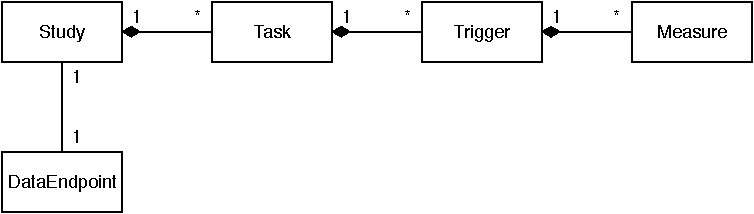
\includegraphics[width=0.8\textwidth]{images/CAMS-UML.pdf}
    \caption{A UML diagram of the \textit{CAMS} Domain Model.}
    \label{fig:cams_uml}
\end{figure}

Concretely, a \textit{Study} holds a set of \textit{Triggers}, which define \textit{when} sampling is carried out, such as by scheduling sampling at  given time each day, or when a certain event is registered, such as entering a specific \textit{GeoFence}\footnote{\url{https://developers.google.com/location-context/geofencing}}. 

Each \textit{Trigger} holds one or more \textit{Tasks}, each of which define which \textit{Measures} should run simultaneously. In addition, a \textit{Task} also defines whether or not data is sampled in the background, or whether the user needs to interact with the device in order to perform sampling. 

Each \textit{Task} holds a set of \textit{Measures} each of which defines what to sample, i.e. which data channel to listen to. Lastly, a \textit{Study} also holds a reference to the \textit{DataEndpoint} specifying which where data ends up, i.e. by uploading it to a server.

An integration for the CAMS Framework will be described later in this thesis. 

\chapter{Theory}
\label{chapter:03}
This chapter will describe the theoretical background for the Mobility Features Package including all the features chosen to be included and how they are computed.
\section{Location Data}
The Navbar Global Positioning System (GPS) is a space-based radio-navigation system developed by The US Office of the Department of Defense \cite{gps-navstar} that provides location data to GPS receivers such as the one found in smart-phones. GPS is capable of delivering information such as latitude and longitude coordinates which indicates where on the Earth's surface the receiver is located, in addition to the altitude, i.e. the distance from the surface. Previously one would have to use a stand-alone GPS tracker as was done by Ashbrook and Starner \cite{using_gps_to_learn_significant_locations} in order to collect this data, but nowadays smart-phone contain GPS receivers which enable users to use a variety of navigation services and applications with their phone alone. From a developer perspective,  tracking location data on the Android- or iOS platform works by using an Application Programming Interface (API) which uses the GPS receiver inside the phone to place it on the Earth geographically. This API allows the streaming of location data in a continuous fashion which is used for navigation such as with Google Maps, where the user's location changes continually and it is important that the user is notified if they have to make a turn in due time. 

\subsection{Measuring Distance}
As mentioned, location data is defined by a latitude- and longitude coordinate which map to a point on the globe, however since the earth is a sphere and not a plane, a standard Euclidean distance metric cannot be used to calculate the distance between two points on the surface of the Earth. A few methods of calculating the distance between GPS coordinates exist, one of the fastest to compute being the Haversine formula \cite{haversine-formula} which calculates the great-circle distance between the two points on a sphere. The Earth is however not exactly spherical, and therefore the Haversine distance is just an approximation that works well when the distance has to be calculated many times, such as when calculating the distance of a path consisting of many points close to each other.

Given the radius of a sphere $r$ and two points on the sphere, $A$ and $B$, the \textit{haversine distance} between the two points can be directly computed as 
\begin{equation}
\label{eq:haversine}
d = 2r \cdot \arcsin \Bigg( \sqrt{\sin^2 \bigg( \frac{lat_B - lat_A}{2} \bigg) + \cos(lat_A) \cdot \cos(lat_B) \cdot \sin^2 \bigg(\frac{ lon_B - lon_A}{2} \bigg)}\Bigg)
\end{equation}


\section{Feature Definitions}
\label{section:definitions}
Here, an overview of the algorithms used by the \textit{Mobility Features Package} will be provided. The overview will not discuss implementation details but will provide precise definitions for how these are computed and the considerations which were made. Most of the features were simple to implement with support for real-time computation and were just a matter of performing arithmetic with regards to distance and time spent and places, however, the ones which need some explanation are outlined in this section. 

The Mobility Features included in the Mobility Features package are a subset of the features described by Saeb et al. \cite{Saeb2015}, Canzian et al. \cite{Canzian2015} and Cuttone et al. \cite{sparse-location-2014} and are outlined in Table \ref{tab:features-nilsson}.

\begin{table}[h]
    \centering
    \begin{tabular}{|p{0.3\textwidth}|p{0.6\textwidth}|}
    \hline
    \textbf{Feature}   & \textbf{Description}                                                                                                  \\ \hline
    Stop               & \textit{A collection of location samples representing visit at a known place with an arrival and departure timestamp} \\ \hline
    Place              & \textit{A cluster of stops found the DBSCAN algorithm}                                                                \\ \hline
    Move               & \textit{A travel between two stops with a path of location samples}                                                   \\ \hline
    Number of Places   & \textit{The number of places visited today}                                                                           \\ \hline
    Home Stay          & \textit{The percentage of the time spent at the home place today}                                                     \\ \hline
    Routine Index      & \textit{The overlap of the time-place distribution that between today and the max 28 previous days}                   \\ \hline
    Location Variance  & \textit{The statistical variance in the latitude and longitude coordinates today}                                     \\ \hline
    Distance Travelled & \textit{The total distance travelled today in meters}                                                                 \\ \hline
    Entropy            & \textit{The entropy of the time-place distribution today}                                                             \\ \hline
    Normalized Entropy & \textit{The entropy normalized the by the max possible entropy. Invariant to the number of places visited today}      \\ \hline
    \end{tabular}
    \caption{The features included in the Mobility Features Package}
    \label{tab:features-nilsson}
\end{table}

When defining a \textit{Place}, several edge cases come to mind such as visiting multiple buildings on a university campus, visiting two stores right next to each other, walking around in a park, i.e. having a large dispersion of the data points. There are likely many more edge cases that exist which have not been considered, but we need to generalize when coming up with a definition. To generalize we define \textit{Stops} using a radius parameter $r_{stop}$ to group data points, and likewise a radius parameter $r_{place}$ to cluster Places. These parameters define the maximally allowed dispersion of the data points which allows us to filter out singular noisy data points. In order to find suitable values for these parameters, a small synthetic dataset was used, and afterward, a real-life dataset from the author moving around in Munich for 9 days was used. No in-depth parameter search was conducted, but the algorithms produce very precise results with the following parameter values:

\begin{equation}
\label{eq:stop-place-radius}
r_{stop} = 25 \text{m}, \quad r_{place} = 25 \text{m}
\end{equation}


In addition we define a date as $d_t$ an the previous date as $d_{t-1}$ in order to define a period is a set of today and it's preceding 28 dates defined as $D = \{d_{t-28}, d_{t-27}, ..., d_{t}\}$\\

\subsection{Location Sample}
A \textit{Location Sample} is a timestamped location and is defined by the tuple $x = (T, l)$ where $T$ is the exact timestamp and $l$ is the Location defined as a geographical point on the globe. The distance between two \textit{Location Samples} $x_a$ and $x_b$ is defined as $\delta(x_a, x_b) = \delta(l_a, l_b)$ and $\delta$ is the \textit{Haversine} distance function.

\subsection{Stop}
Finding \textit{Stops} is done by traversing every \textit{Location Samples} in temporal order, i.e. the timestamp is used. The \textit{Stops} for a given date is found by clustering \text{Location Samples} on that date based on time and distance. The set of \textit{Stops} found for the period $D$ is defined as

\begin{equation}
\label{eq:feature-stops}
S = \{s_1, s_2, ..., s_{|S|}\} \;| \; s_i = (T_{arr}, T_{dep}, l)
\end{equation}

The triple $(T_{arr}, T_{dep}, l)$ denotes the arrival timestamp, the departure timestamp and the cluster location for the Stop $s_i$, respectively. Stops are found using Algorithm \ref{algo:stops}.

\begin{algorithm}[H]
\SetAlgoLined
\algorithmicrequire{ set of time ordered data points, $X$}\\
\algorithmicensure{ set of stops, $S$}\\

 $S \leftarrow \{ \}$\;
 \While{at least one point $x'$ remains in $X$}{
    $X \leftarrow X - x'$;\\
    $s \leftarrow \{ x' \}$;\\
    \For{$x \in X$}{
        \eIf{$\delta($x$, $s$) \leq r_{stop}$}{
            $s \leftarrow s \cup \{ x \}$;\\
            $X \leftarrow X - x$;
        }{
            $S \leftarrow S \cup \{ s \}$;\\
            break \textbf{for}-loop;
        }
    }
 }
 \textbf{return} $S$\;
 \label{algo:stops}
 \caption{Find Stops}
\end{algorithm}

\subsection{Place}
\textit{Places} can now be found by applying the \textit{DBSCAN} algorithm to the \textit{Stops} found. All the Stops today in the period $D$ should used to identify places, for reasons explained in subsection \ref{sub:hour-matrix}. That is, given a set of Stops $S$ for the period $D$, the set of Places $P$ for the period $D$ is defined by Equation \eqref{eq:feature-places}.

\begin{equation}
\label{eq:feature-places}
P = {p_1, p_2, ..., p_N} \;|\; p_i = \{s_1, s_2, ..., s_{|p_i|}\}
\end{equation}

The procedure for finding Places defined in Algorithm \ref{algo:places}.

\begin{algorithm}[H]
\SetAlgoLined
\algorithmicrequire{ set of stops, $S$}\\
\algorithmicensure{ set of places, $P$}\\
    $L = DBSCAN(S)$ where $s_i$ has label $l_i$;\\
    \textbf{group} each stop $s_i \in S$ by $l_i$;\\
    $S' = \{s_i \;|\; l_i \geq 0\}, \;|S'| = N$;\\
    $p_i = S'_i$ where each stop $s \in S'_i$ has the label $l_i$;\\
    \textbf{return} $P = \{p_i : i = 0, ..., N\}$;\\
 \label{algo:places}
 \caption{Find Places}
\end{algorithm}

\subsection{Move}
\textit{Moves} for a given can be calculated using the \textit{Stops}- and the \textit{Location Samples} from that date. The \textit{Moves} are found by going through each \textit{Stop} and calculating the distance between the current \textit{Stop} and the following \textit{Stop} by going through all the \textit{Location Samples} which were sampled in the time interval between these the \textit{Stops}. These points form the path which was taken between the two \textit{Stops} and the path is used to calculate the exact distance traveled.

A set of \textit{Moves} is defined as 

\begin{equation}
\label{eq:feature-moves}
M = \{m_1, m_2, ..., m_{|M|}\} \;| \; m_i = (s_a, s_b, X_i), X_i = \{x_1, x_2, ..., x_{|X_i|}\}
\end{equation}

is a set of time-ordered Location Samples. Moves are found using the following procedure outlined in Algorithm \ref{algo:moves}.

\begin{algorithm}[H]
\SetAlgoLined
\algorithmicrequire{ set of stops, $S$, set of time ordered data points, $X$}\\
\algorithmicensure{ set of moves, $P$}\\
    $M = \{ \}$\;
    \For{$s_i \in S$}{
    $X_i = x$ for which $s_{i}.departure \leq x.timestamp \leq s_{i+1}.arrival$;\\
    $d_i = \sum_{x_j \in X_i} \delta(x_j, x_{j+1})$;\\
    $m_i = (s_i, s_{i+1}, d_i)$;\\
    $M = M \cup \{m_i\}$;\\
    }
    \textbf{return} $M$;
 \label{algo:moves}
 \caption{Find Moves}
\end{algorithm}


\subsection{Hour Matrix}
\label{sub:hour-matrix}
The Hour Matrix is an auxiliary feature used to compute the \textit{Home Stay} and \textit{Routine Index} feature. A matrix with 24 rows, each row representing an hour in a day, and columns equal to the number of places. The \textit{Hour Matrix} represents the time-place distribution for the user during a day.
\begin{figure}
    \centering
    \begin{tabular}{|l|l|l|l|l|}
    \hline
    \textbf{}        & \textbf{Place \#1} & \textbf{Place \#2} & \textbf{...} & \textbf{Place \#N} \\ \hline
    \textbf{00 - 01} &                    &                    &              &                    \\ \hline
    \textbf{01 - 02} &                    &                    &              &                    \\ \hline
    \textbf{...}     &                    &                    &              &                    \\ \hline
    \textbf{16 - 17} &                    &                    &              &                    \\ \hline
    \textbf{17 - 18} &                    &                    &              &                    \\ \hline
    \textbf{18 - 19} &                    &                    &              &                    \\ \hline
    \textbf{...}     &                    &                    &              &                    \\ \hline
    \textbf{23 - 00} &                    &                    &              &                    \\ \hline
    \end{tabular}
    \caption{An \textit{Hour Matrix}}
    \label{fig:time-table}
\end{figure}

This matrix is constructed from all the \textit{Stops} on a given day, each of which belong to certain \textit{place} and has an \textit{arrival} and \textit{departure} timestamp. From this, it can be calculated exactly which hour slot(s) to fill out and the duration to fill that slot with. For simplicity, we define a couple of constraints on the \textit{Hour Matrix}:

\begin{itemize}
    \item The \textit{Hour Matrix} has exactly 24 rows, each representing 1 hour in a day.
    \item The number of columns represents the number of \textit{Places} for the period. 
    \item An entry represents the portion of the given hour-slot that was spent at a given \textit{Place}.
    \item Each row can maximally sum to 1.
\end{itemize}

Formally, given a period ($D$) for which the number of \textit{Places} is given as $N$ the \textit{Hour Matrix} $\mathsf{H}$ for today ($d_t$) is defined as:

\begin{equation}
\label{eq:feature-hour-matrix-def}
\mathsf{H}(d_t) \in [0,1]^{24 \times N}, \sum_{j=1}^N \mathsf{H}^{d_t}_{i,j} \leq 1
\end{equation}

Given an array of \textit{Hour Matrices} for a period $D' = D - d_t$ (i.e. the historical dates preceding today $d_t$) the \textit{Routine Matrix} is defined as the average entry for each \textit{Hour Matrix} given in Equation \eqref{eq:feature-hour-matrix-mean}. Here, $|D'|$ defines the number of preceding dates for which $1 \leq |D'| \leq 28$ holds.

\begin{equation}
\label{eq:feature-hour-matrix-mean}
\mathsf{H}^{\mu} (D) _{i,j} = \sum_{k=0}^{|D'|} \frac{1}{|D'|} \mathsf{H}(d_{|D'|-k})_{i,j}
\end{equation}

Given a Stop $s$ with arrival $T_{arr}$ and departure $T_{dep}$ the hour matrix as follows:

Let $i = hour(T_{arr})$, $j = hour(T_{dep})$ and $\Delta_ T(\cdot)$ is the function for calculating the duration in hours.

\begin{equation}
\label{eq:feature-hour-matrix-computation}
\mathsf{H}_{i,p} \leftarrow \mathsf{H}_{i,p} + T
\end{equation}

If $i = j$ then $T = \Delta_T (T_{dep} - T_{arr})$, otherwise the following algorithm is applied:

\begin{equation}
\label{eq:feature-hour-computaion2}
\mathsf{H}_{i,p} = 1 - T
\end{equation}

Where the value of $T$ depends on the variable $k = i$ up to $j$:

\begin{equation}
\label{eq:feature-hour-computaion3}
T(k) =
\begin{cases}
    \Delta_T (T_{dep} - T_{arr})    & \text{if $i = k = j$} \\
    1 - (hour(T_{arr}) - T_{arr})   & \text{if $i = k < j$} \\
    1                               & \text{if $i < k < j$} \\
    hour(T_{arr}) - T_{arr}         & \text{if $i < k = j$}
\end{cases}
\end{equation}


\subsection{Home Stay}
The \text{Home Stay} feature indicates the percentage of time spent at the Home cluster, out of all the time of the day. In the literature, the home cluster is defined as the cluster which the user spends the most time at between 00:00 and 06:00. In the work by Saeb et al. and Canzian et al. \cite{Saeb2015, saeb2016, Canzian2015} the home cluster was evaluated over the duration of the whole study, however we define it on a daily basis since the home cluster may change from day to day. Formally, the \textit{Home Place} $p_h (d_t)$ for the date $d_t$ where the index $h$ is found using Equation \eqref{eq:feature-home-place}.

\begin{equation}
\label{eq:feature-home-place}
h = \operatorname*{argmax}_n \sum_{m=1}^{6} \sum_{n=1}^{N}  \mathsf{H}(d_t)_{m,n}
\end{equation}

In the work by Saeb et al. \cite{Saeb2015} and Canzian et al.\cite{Canzian2015} it is not stated how this would be calculated for an incomplete day. It was chosen to  use the time elapsed from midnight until the departure of the last known Stop. The Home Stay feature is computed using \eqref{eq:feature-home-place} where the duration of a stop $s$ will be denoted $\Delta T (s)$ and similar the duration spent at a place $p$ is defined as $\Delta T (p)$.

\begin{equation}
\label{eq:feature-home-place}
\Delta T(p_{h} (d_t) )= \frac{\sum_i \Delta_T (s_i) \;|\; s_i \in p_h (d_t)}{T_{now} - T_{0}}
\end{equation}

Where $T_{now}$ is the departure time of the last known stop, and thus $T_{now} - T_0$ is the time elapsed since 00:00:00 today.

\subsection{Total Distance Travelled}
First we define the distance of a Move $m_i$ as the sum of all the distances in the 'chain' of points in $X_i$, i.e.

\begin{equation}
\label{eq:feature-move-computation}
\delta (m_i)  = \sum_{j=1}^{|X_i|-1} \delta (x_j, x_{j+1})
\end{equation}

The \textit{Total Distance Travelled} for a date $d_t$ is defined as 

\begin{equation}
\label{eq:feature-total-distance}
\delta (d_t) = \sum_{i=1}^{|M|} \delta (m_i)
\end{equation}

where $M$ refers to the moves on date $d_t$.

\subsection{Number of Places}
By using the DBSCAN algorithm to cluster a set of Stops, each Stop is given a cluster label, either being non-negative if it belongs to a cluster, or the label -1 if it is considered noise. The \textit{Number of Places} is therefore defined as the size of the set of non-negative cluster labels $K = \{k_1, k_2, ..., k_N\}$, i.e.

\begin{equation}
\label{eq:feature-num-places}
N = |K|
\end{equation}

\subsection{Location Variance}
Defined by Saeb et al. \cite{Saeb2015}, the Location Variance is defined as the natural logarithm to the variance of the latitude and longitude coordinates summed together: 

\begin{equation}
\label{eq:feature-log-var}
\sigma^2 = \log (\sigma_{lat}^2 + \sigma_{lon}^2)
\end{equation}

The logarithm is applied in order to compensate for the skewness in the location distribution of location variances across users.

\subsection{Entropy and Normalized Entropy}
Within the field of Information Theory, entropy is described in MacKay \cite{information-theory} as a quantity associated with a random variable, and can be interpreted as the average level of \textit{information} contained within the outcomes of that variable. 

The Entropy $H(X)$ of the set of outcomes $X = \{x_1, x_2, ..., x_n\}$ is defined as

\begin{equation}
\label{eq:feature-entropy}
H(X) = -\sum_{i=1}^{n} p(x) \log p(x)
\end{equation}

The Entropy is maximised if $p(x) = \frac{1}{n}$ for all $x \in X$, i.e. all outcomes are equally likely. If this is the case, the Maximum Entropy becomes 

\begin{equation}
\label{eq:feature-entropy-max}
H_{max}(X) = - \sum_{i=1}^{n} p(x) \log p(x) = - \sum_{i=1}^{n} \frac{1}{n} \log \frac{1}{n} = -n \frac{1}{n} \cdot -\log n = \log n 
\end{equation}

We define the Normalized Entropy as the Entropy $H$ normalized using the maximum possible entropy $H_{max}$:

\begin{equation}
\label{eq:feature-normalized-entropy}
H_N(X) = \frac{H(X)}{H_{max}(X)} \in [0,1]
\cdot -\log n = \log n 
\end{equation}

The Normalized Entropy (NE) makes it easier to compare Entropy values of different distributions since they all reside on the same scale, being a scalar value between  0 and 1. A NE value near 1 indicates that the $X$ follows a uniform distribution where every outcome is equally likely. A small NE value indicates that the distribution is very skewed, with certain outcomes having very high likelihood and some having much lower likelihood. 

In the context of user mobility, we can view the time user spends at a certain place as the outcome of the place variable, i.e. 

\begin{equation}
\label{eq:feature-normalized-entropy-places}
H(P) = - \sum_{i=1}^{n} Pr(p_i) \log Pr(p_i)
\cdot -\log n = \log n 
\end{equation}

and by using \eqref{eq:feature-normalized-entropy} and \eqref{eq:feature-normalized-entropy-places} we ge the Normalized Entropy for the time-place distribution:

\begin{equation}
\label{eq:feature-normalized-entropy}
H_N(P) = \frac{H(P)}{H_{max}(P)} \in [0,1]
\end{equation}

where $P$ is the set of places visited today and $Pr(p_i)$ refers to the time spent at place $p_i$ today. It must holds that $Pr(p) > 0$ for $p \in P$, otherwise the term $\log P(p_i)$ cannot be evaluated since $\log(0)$ is undefined. The concept of NE gives us a tool to say something about where the user spends their time; a high NE value indicates they spend their time uniformly among the places, whereas a low value indicates that the user spends most of their time at very few places. 

\subsection{The Routine Index}
\label{sub:routine-index}
The \textit{Routine Index} describes how similar the place-time distribution of a given day is, compared to previous days for a period $D$. The place-time distribution for a day is defined by how much time was spent for each of the 24 hours, at different places. For computing the Routine Index, a period length of 28 days was chosen, which means the \textit{Routine Index} of today describes how similar today was to each day during the last month. The implementation by Canzian et al. \cite{Canzian2015} involved using a different modelling approach and was therefore very complicate to compute.  Therefore, a more straightforward definition of the Routine Index was chosen. To the best of our knowledge this definition defined in Equation \eqref{eq:feature-routine-index} in conjunction with the concept of an Hour Matrix is novel, and models the feature as a similarly measure between two Hour Matrices. More exact, the Routine Index is a similarity measure between the Hour Matrix today and the 'average' Hour Matrix for the last 28 days. The result of the similarity measure is a scalar between 0 and 1 - a low value indicating a small degree of overlap and a high value indicating a high degree of overlap. 


In general, peoples' habits will inevitably change somewhat over time, and if one compares the routine of a certain person now to what their routine looked like a year ago, it is not unlikely to be very different. However just because someone changes their routine over time, does not mean they don't currently possess one. Therefore it was chosen to base the \textit{Routine Index} on the last 4 weeks (28 days) of data in order to base the routine overlap on more recent days. 

The feature can therefore indirectly be computed from the Stops of the last 28 days which means only the Stops are necessary to store. In a field study (described in chapter \ref{chapter:06}), the author was found to have had just around 20 stops per day which amounts to under 600 Stops for a 4 week period. Computing the feature requires the Places to be found, i.e. to run DBSCAN on the Stops, and can result in the feature being expensive to compute. However, 600 data points is a manageable number to work with.

The overlap function produces a matrix $\mathsf{O}$ given two matrices $\mathsf{A}$ and $\mathsf{b}$ of equal dimensions:

\begin{equation}
\label{eq:overlap-function}
    \mathsf{O}(\mathsf{A}, \mathsf{B}) = \sum_{i=1}^{24} \sum_{j=1}^{N} \min (A_{ij}, B_{ij}) \;|\; A_{ij} \geq 0, B_{ij} \geq 0
\end{equation}

The maximum potential overlap is limited by the minimum of the two matrix sums, this is reflected in \eqref{eq:max-overlap}.

\begin{equation}
\label{eq:max-overlap}
    \mathsf{O}_{max}(\mathsf{A}, \mathsf{B}) = \min (\sum \mathsf{A}, \sum \mathsf{B})
\end{equation}

The \textit{Routine Index} for today $d_t$ given the historical dates $D$, is defined as the overlap normalized by the maximum potential overlap of today's Hour Matrix and the Routine Matrix (Equation \eqref{eq:feature-routine-index}).

\begin{equation}
\label{eq:feature-routine-index}
r(d_t, D) = \frac{\sum (\mathsf{H}(d_t) \cap \mathsf{H}^{\mu} (D) )}{\min \Big(\sum \mathsf{H}(d_t), \sum \mathsf{H}^{\mu} (D) \Big)}
\end{equation}


Equation \eqref{eq:feature-routine-index} uses the smallest sum of the two matrices to normalize the overlap, which is done to avoid punishing days with gaps in the data too much. Otherwise one could simple define the maximum potential overlap as 24 hours. However travels between places are not reflected in the Hour Matrix and therefore there will be gaps in the data. Ideally, travels such as commutes would also be included in the Hour Matrix by using both stops and moves to construct it.
Below, in Figure \ref{routine-matrix-1} and Figure \ref{routine-matrix-1} are shown two examples of overlap matrices computed, and the resulting Routine Indices.

\begin{figure}[h]
    \centering
    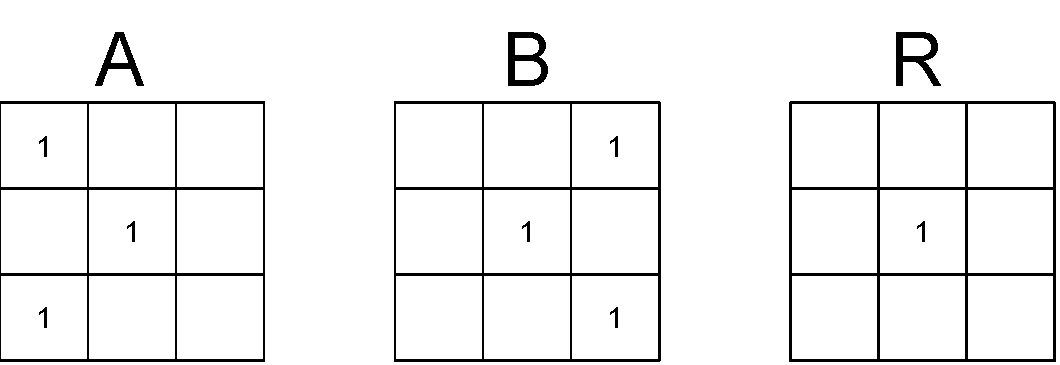
\includegraphics[width=\textwidth]{images/routine-numbers-1.pdf}
    \caption{An example of the matrix R is computed with the overlap function of A and B. Here only 1 entry overlaps}
    \label{fig:routine-matrix-1}
\end{figure}

For Figure \ref{fig:routine-matrix-1} the Routine Index becomes 

\begin{equation}
RI = \frac{1}{1 + 1 + 1} = \frac{1}{3}
\end{equation}

\begin{figure}[h]
    \centering
    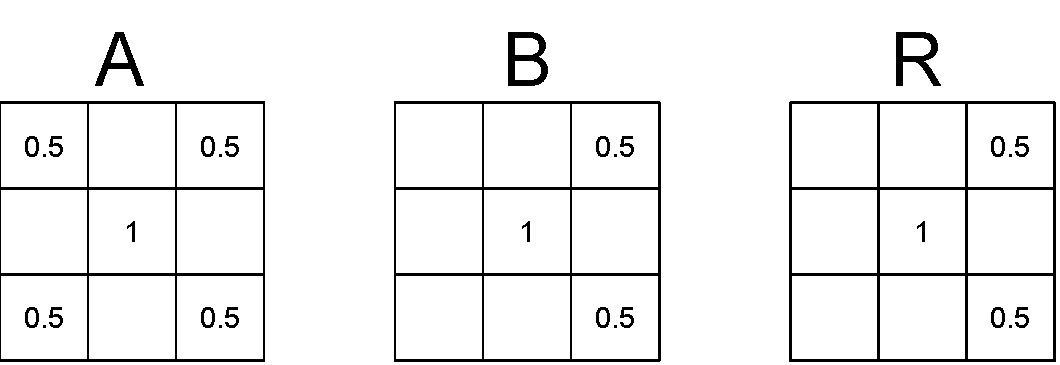
\includegraphics[width=\textwidth]{images/routine-numbers-2.pdf}
        \caption{An example of the matrix R is computed with the overlap function of A and B. Here several entries overlap}
    \label{fig:routine-matrix-2}
\end{figure}

For Figure \ref{fig:routine-matrix-2} the Routine Index becomes

\begin{equation}
RI = \frac{1 + 2\cdot 0.5}{2} = 1
\end{equation}



\chapter{Software Design}
\label{chapter:04}
This chapter deals with the design of the software architecture on a high level and will describe the package in terms of its components. Components may sometimes be referred to as \textit{classes} and vice versa, where \textit{component} refers to the general term and \textit{class} refers to the programming language equivalent of a component.

\section{Requirements and Design Choices}
The functional requirements the package should meet, and how these are met will be described in this section. Fundamentally the package should support the computation of the features described in \ref{chapter:03} however there are several layers to achieving this, including the following:

\begin{itemize}
    \item Saving and loading of Location Samples on the device
    \item Computing intermediate features from Location Samples
    \item Saving and loading Stops and Moves on the device
    \item Computing the features
\end{itemize}

Saving and loading of Location Samples is necessary in order to not lose data. When an application tracks location data for a pro-longed period of time, i.e. a whole day, it will risky to keep all the collected data in RAM, since all data is lost if the app is killed by accident either by the OS or the user. For computing the Routine Index it was necessary to store historical data, in order to compare days. Intermediate features made this possible by bringing the storage requirements down significantly, compared to storing raw Location Samples on the device. A normal day of tracking could result in up to 18,000 Location Samples which is quite a lot of data considering the algorithms need up to 28 days of data. In addition, converting a dataset of raw Location Samples into Stops also made the computation for finding Places, and thereby many of the mobility features, much cheaper. Lastly, computing mobility features should be possible at any time, even if the day is incomplete. This has been taken care of by the definitions made in Chapter \ref{chapter:03} by redefining features such that they can be evaluated on incomplete days.

\subsection{Storing and Loading}
Since historical data is a major factor in computing the features, it was decided to include an easy way for the programmer to store and load Location Samples. To store objects in an Object Oriented Language serialization \footnote{\url{https://www.martinfowler.com/eaaCatalog/serializedLOB.html}} can be used, which is act of transforming an object into a graph of smaller objects in a data format which can be written to a file. A serialized object, in contrast to an entity stored in database is already pre-assembled. In a database this assembly happens via joins since the object is spread over multiple tables. The database may store the object more efficiently, but it does not come pre-assembled. This is analogous to how a set of Legos blocks comes in a box rather than already being pre-assembled. While traditional databases usually scale better than serialization they come with an overhead cost of being time consuming to set up properly. For this reason serialization was chosen in favor of databases,  since the project was small. In addition it is also very easy to import serialized objects into other programming languages, such as Python for data analysis. 

\subsection{Data Format}
The data format used was JSON (JavaScript Object Notation) which is a very common, human-readable data format that uses key-value pairs to store data. A JSON object can be stored in a database, or it can be transformed to a string in order to be stored. It was chosen to simply transform JSON objects to a string and write them to a local file, rather than storing the information in a database on the phone. JSON supports a limited number of simple data types, such as strings, numbers, booleans, arrays, objects and null values. This means that in order to translate a runtime object to JSON, all of the object's data must be serializable. Serialization therefore requires components which are to be serialized to be converted into some representation which is purely consisting of these simpler data types.

\subsection{Computing Features}
The road from starting with a blank slate to computing mobility is depicted in the flowchart in Figure \ref{fig:flowchart-features}. First the programmer needs to initialize data collection and save the collected samples with some frequency. Exactly how this is done is left the programmer. When feature computation is requested, the stored data including Location Samples, Stops and Moves are loaded into memory. The Mobility Context for today is computed from this data, and afterwards it is checked whether or not prior contexts should be used. If so, then the historical Stops and Moves are used to generate these, and they are added to the Context of today. In any case, today's Context is returned to the method caller.

\begin{figure}
    \centering
    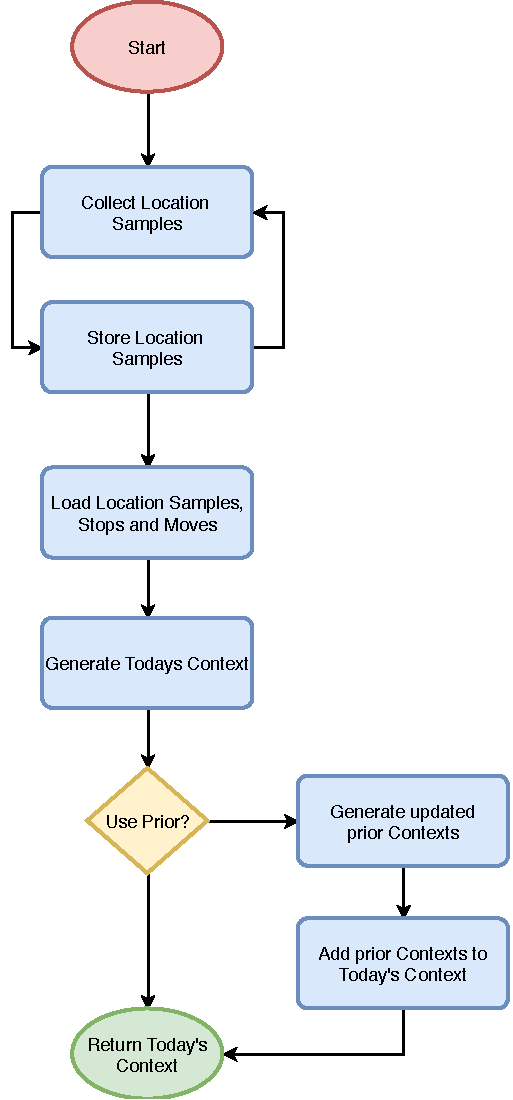
\includegraphics[width=0.5\textwidth]{images/diagrams/api-flowchart.pdf}
    \caption{The flowchart for computing mobility features using historical data}
    \label{fig:flowchart-features}
\end{figure}



\section{Domain Model}
The domain model provides clarity and direction for a software system, even on a small scale such as in a library. In this section the design choices of the data model will be discussed.

\subsection{Data Model Overview}
In order to capture the data model in an object-oriented programming language, a UML diagram was maintained as the implementation went along in order to keep track of relationships between the classes. 
% As a general rule of thumb, all the fields were made public including those required by the constructors, and the methods of the classes were all \textit{getters}, i.e. \\

\subsubsection*{GeoPosition}
A \textit{GeoPosition} is defined by a geographical \textit{latitude} and \textit{longitude} and represents a 2D position on the Earth's surface.

\subsubsection*{Location Sample}
A \textit{Single Location Data Point} is a time-stamped \textit{Location}. By having a time-stamp, a collection of Location Samples may be ordered and grouped by the time of day. In essence, the class is a Data Transfer Object (DTO) \footnote{\url{https://martinfowler.com/eaaCatalog/dataTransferObject.html}} which is used to transfer GPS data from an arbitrary Location plugin to the \textit{Mobility Features Package}.

\subsubsection*{Hour Matrix}
An \textit{Hour Matrix} is a matrix with 24 rows and columns equal to the number of places of some period. The \textit{Hour Matrix} class is used to calculate the \textit{Routine Index} feature, as well as to identify the \textit{Home Cluster}, which is the place most visited during 00:00 and 06:00. An Hour Matrix is constructed from a list of \textit{Stops} which all have the same date.

\subsubsection*{Stop}
A \textit{Stop} is constructed from a centroid of a data point cluster (i.e. a Location) in addition to an arrival- and a departure timestamp, and a place ID indicating which place it belongs to.

\subsubsection*{Place}
A \textit{Place} is constructed from a place ID, as well as a collection of \textit{Stops} belonging to that \textit{Place}. 

\subsubsection*{Move}
A \textit{Move} is constructed from a pair of \textit{Stops} as well as the set of \textit{LocationSamples} which were sampled in between the two \textit{Stops} which is the path the user took between the two \textit{Stops}.

\subsubsection*{Mobility Context}
A \textit{Mobility Context} is a collection of features which are derived from a set of intermediate features, where the \textit{Stops} and \textit{Moves} are from a specific date. The \textit{Places} is derived from multiple dates for reasons which will be explained in the implementation details. In addition, a set of \textit{Mobility Contexts} from previous dates can be provided as an optional parameter. A Mobility Context contains the mobility features, although the \textit{Routine Index} is only available if an array of the set of \textit{Mobility Contexts} was provided as a parameter, which is due to the feature depending on the data from previous days in order to compare them.

\subsubsection*{GeoSpatial (Interface)}
This interface will impose a getter-method for the GeoPosition of the class which implements it. This allows the Haversine distance to be calculated between objects of different types.

\subsubsection*{Serializable (Interface)}
This interface will impose a serialization and de-serialization method for converting between a language object and a JSON object. The interface will allow the MobilitySerializer component as previosly discussed to more easily implement serialization in a generic manner which is disucssed in Chapter \ref{chapter:05}.

\subsection{UML Diagram and Discussion}

\begin{figure}[h]
    \centering
    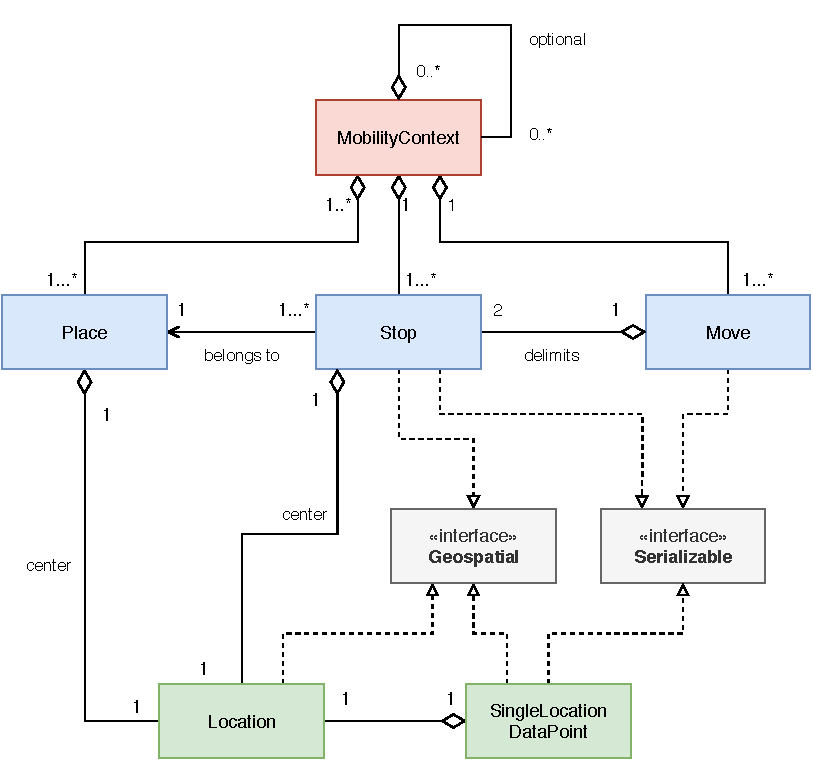
\includegraphics[width=0.7\textwidth]{images/diagrams/uml.pdf}
    \caption{UML diagram for the classes used in the \textit{Mobility Features Package}}
    \label{fig:my_label}
\end{figure}

The data model could be modified such that a Place contained a list of \textit{Stops} made at that place, rather than using both \textit{Places} and \textit{Stops} for instantiation of \textit{Mobility Context}. This would mean grouping the \textit{Stops} by Place rather than date, and would require filtering to take place every time a \textit{Mobility Context} object is created, to remove all Stops, not on that specific date. In a real-world scenario the application developer will likely have the Location Samples for the current day available, and from those the \textit{Stops} today can be generated which means no filtering is required. Grouping \textit{Stops} into places would however lead to a nicer data model, but a design choice was made in favor of less computation. 



\section{System Design}
The core idea of the \textit{Mobility Feature Package} is to provide a very simple programming interface such that computing features can be done with very few lines of code. This requires closing of the internal working of the package off, such that the programmer has very limited ways in which he/she can interface with it. The design of the package API went through two main iterations which consisted of many smaller iterations. Mainly, the difference between the final iteration and the earlier iterations is the amount of code required for managing historical data that the programmer has to write. Early iterations put the responsibility on the application programmer to manage historical data. After developing the field study app discussed in chapter \ref{chapter:06} it was decided to move most of this logic inside the package; it became glaringly apparent that the package was too cumbersome to use. The final iteration is the one discussed in this thesis including the choices and lessons learned on the way of designing and developing it. 


\subsection{Component Overview}
Figure \ref{fig:component-diagram-internal} displays how the final iteration looks like as a software system: The main component is the \textit{Context Generator} component which is the interface that the programmer will use. This component exposes two interfaces to the programmer allowing the user to store their collected \textit{LocationSamples} as well as generate a \textit{Mobility Context} that contains the daily features. The two exposed interfaces are provided by the programmer through mobile application. The \textit{Context Generator} is also responsible for storing and loading data via the \textit{Mobility Serializer} component, here the \textit{Serializable} type refers to any data type that needs to be stored as historical data.

\begin{figure}[h]
\centering
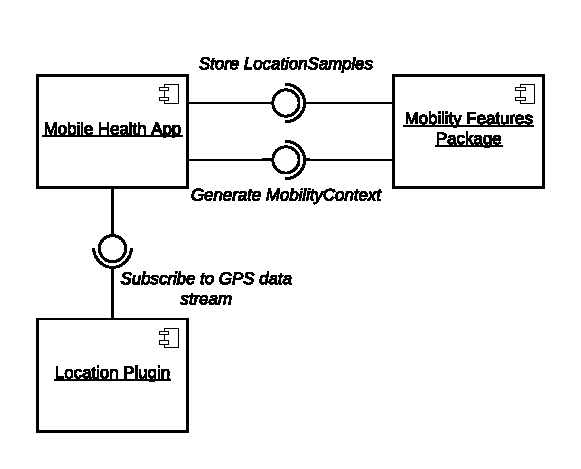
\includegraphics[width=\textwidth]{images/diagrams/component-external.pdf}
\caption{Component diagram for the \textit{Mobility Feature Package} from an internal point of view}
\label{fig:component-diagram-external}
\end{figure}

Figure \ref{fig:component-diagram-external} shows the external software system that includes the mobile application using the package. Another design choice is reflected in this figure which is the usage of an external location plugin which must be done by the programmer. This means task the programmer has to collect their own location data through their location plugin which will collect location \textit{Data Transfer Objects} (DTOs) \cite{fowler-PEEA} [p. 401]. These objects hold location data, i.e. latitude, longitude, and a timestamp and can be converted to \textit{LocationSamples} and saved through the \textit{Mobility Feature Package.}
Two reasons led to this decision, the first of which being that the Mobility Features Package becomes more loosely coupled and modular. The second reason relates to maintenance; if the package was to implement location data collection then it becomes harder to maintain since any change to the location plugin would imply changes to the Mobility Features Package as well. 

\begin{figure}[h]
\centering
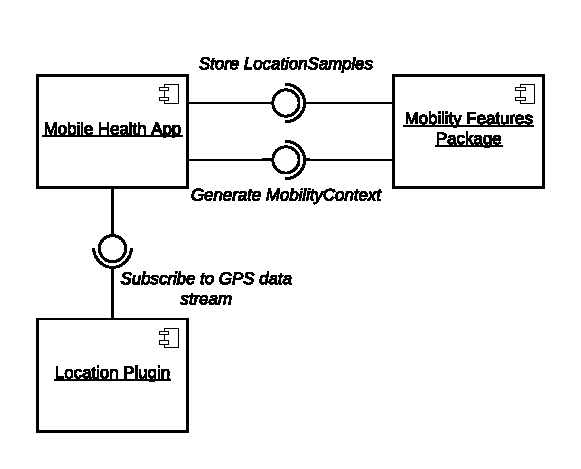
\includegraphics[width=\textwidth]{images/diagrams/component-external.pdf}
\caption{Component diagram for the \textit{Mobility Feature Package} from an internal point of view}
\label{fig:component-diagram-external}
\end{figure}


\subsection{Sequence Overview}
To display the interactions between the components, sequence diagrams are used. Figure \ref{fig:sequence-diagram-external} shows the system from an external point of view, where the application subscribes to location updates via the location plugin, saves location data via the Mobility Features Package and generates a Mobility Context through it. 

\begin{figure}[h]
\centering
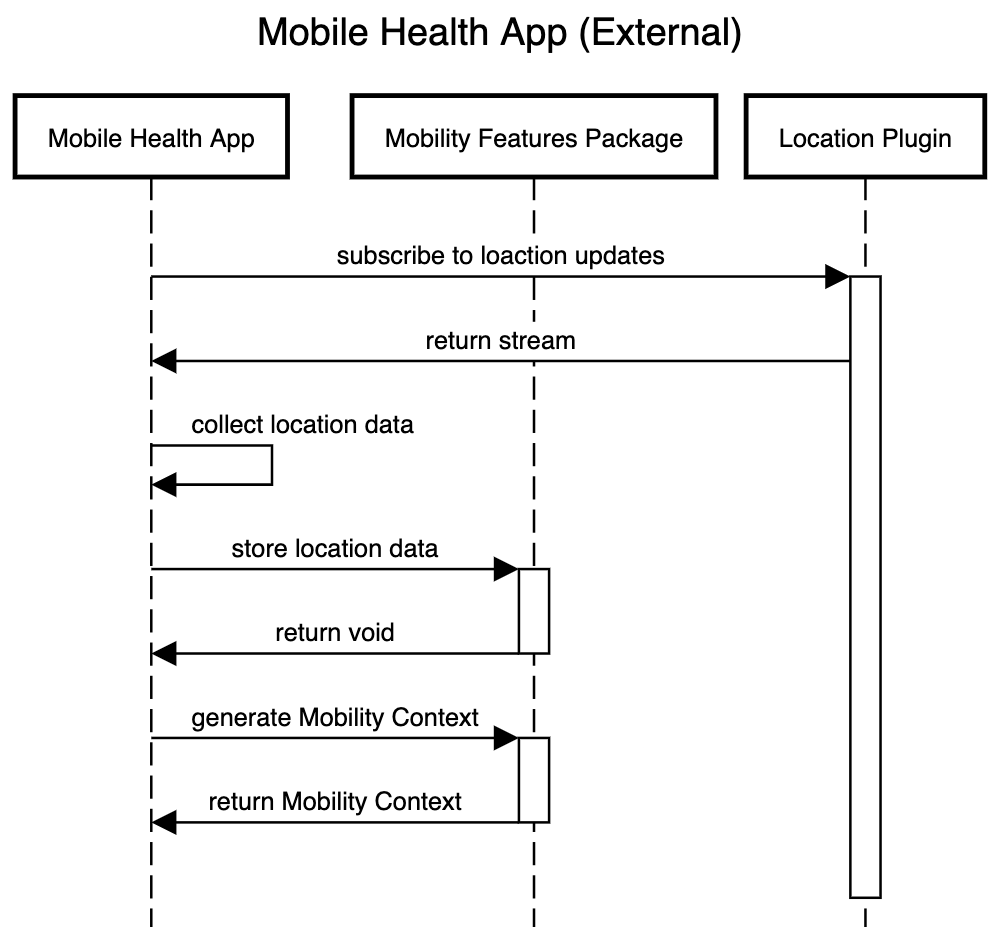
\includegraphics[width=\textwidth]{images/diagrams/sequence-external.png}
\caption{Component diagram for the \textit{Mobility Feature Package} from an internal point of view}
\label{fig:sequence-diagram-external}
\end{figure}

From an internal point of view, the \textit{Context Generator} component calls the \textit{Mobility Serializer} for storing and loading historical data, uses the loaded data to generate a \textit{Mobility Context} by calling the MobilityContext component.
\begin{figure}[h]
\centering
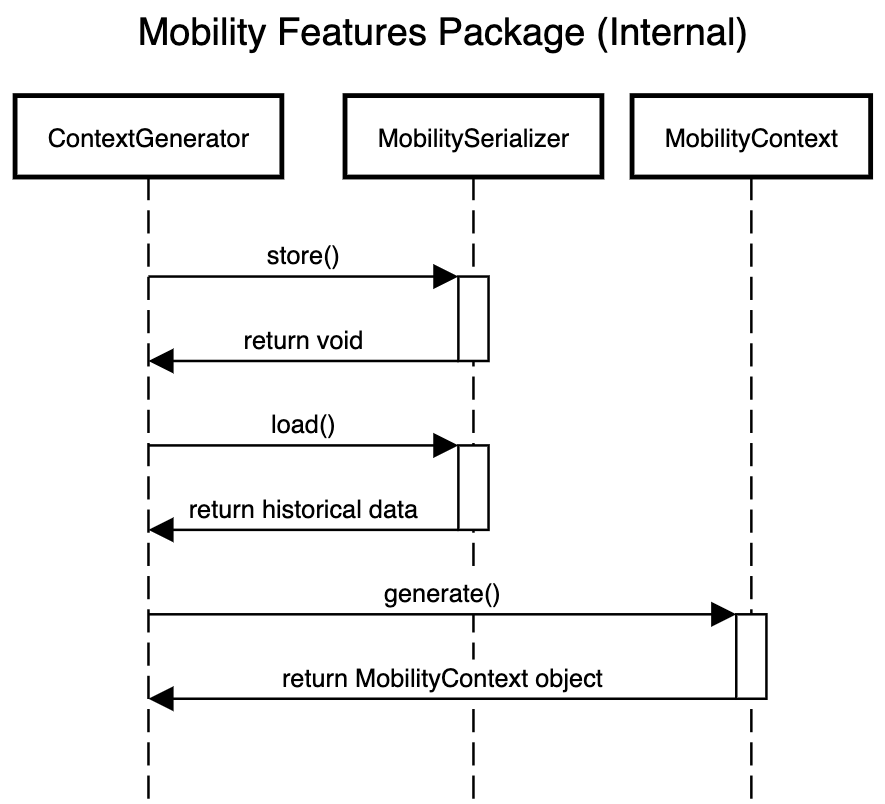
\includegraphics[width=\textwidth]{images/diagrams/sequence-internal.png}
\caption{Sequence diagram for mobile health application using the Mobility Features Package, i.e. viewed externally from the package}
\label{fig:sequence-diagram-external}
\end{figure}


\chapter{Flutter Implementation}
\label{chapter:05}
The final product allows the programmer to compute mobility features with the following 3 lines of code displayed in Figure \ref{fig:code-example-intro}. This chapter will describe how the package design described in Chapter \ref{chapter:04} was implemented in Flutter such that this succinct code interface was achieved. 

\begin{figure}[h]
    \centering
    \begin{minted}{dart}
    /// Collect data with a location plugin
    List<LocationSample> locationSamples = ///

    /// Store data via the package
    await ContextGenerator.saveSamples(locationSamples);
    
    /// Compute Features via the package
    MobilityContext context = await ContextGenerator.generate();
    \end{minted}
    \caption{All the three lines of code necessary for the application developer to write}
    \label{fig:code-example-intro}
\end{figure}



\section{Flutter, Packages and Plugins}
Flutter is a cross-platform app development framework developed by Google and released in 2018. It allows an application programmer to write a mobile application using a single codebase written in the Dart programming language, and compile this source code to a native Android and iOS application. This has the clear advantage of reducing the amount of labour needed to produce mobile applications which most of the time need to be released on both platforms. Packages and Plugins are the Flutter equivalent of a software library which is hosted on the Dart package manager at \url{pub.dev}, the Mobility Features Package is hosted at \url{pub.dev/packages/mobility_features}. 

\subsection{Why Flutter?}
It was chosen to implement the package in Flutter for several reasons: Firstly it is cross-platform, meaning the same code base can compile to both Android and iOS. For this reason one could also have chosen other frameworks such as React Native\footnote{\url{https://reactnative.dev/}} developed by Facebook. The author was employed at CACHET who uses Flutter for mobile development. An example of a CACHET PhD project is \cite{mubs-rohani}. In addition, the author had already authored many packages\footnote{\url{https://pub.dev/publishers/cachet.dk/packages}} for the CARP Mobile Sensing Framework by CACHET.

\subsection{Packages and Plugins}
A flutter \textit{package} is a library containing Dart pure code that enables the creation of modular code that can be shared easily. A package declares the package name, version, author, and so on (see Figure \ref{fig:pubspec}, and secondly a source code directory named \verb|lib|. It is relevant to develop a package when common functionality is to be shared among applications, and the functionality can be computed in the Dart programming language alone. The \textit{Mobility Features Package} is a Flutter package that contains a collection of algorithms that provides an application programmer with object-oriented abstractions that allows him/her to calculate relevant features for a mobile health application. 

Whenever a functionality is wanted which is only available through a native API, such as the camera or battery level, a \textit{plugin} is used instead. In contrast to a package, a plugin contains three codebases: Flutter (Dart), Android (Kotlin/Java), and iOS (Swift/Objective C). The Dart codebase contains an implementation which can be called from a Flutter app, and in turn calls the implementation in the Android environment and the iOS environment (whichever platform the device runs). It does so by transporting data between the platforms, which means no real computation is performed in the Dart environment; the Dart implementation simply invokes a method in the native environment, the native environment performs the computation, or data collection, and then sends back an answer. For transporting data between the native environment and the Dart environment, messaging channels are used, namely \textit{MethodChannels} and \textit{EventChannels}. A \textit{MethodChannel} is used for communicating when data is to be transferred on a whenever a method is invoked. In contrast to this, the \textit{EventChannel} allows streaming data from the native environment every time an event is triggered in the native environment, such as when a sensor picks up on a new data point. A Location API plugin which streams location data continuously uses an \textit{EventChannel}.

This method invocation library is referred to as a \textit{plugin} within the Flutter world, in contrast to a \textit{package} which simply invokes other Dart code and as such contains no platform-specific source code.  The Location API, available on both iOS and Android, will not be invoked directly from this package since that would require it to be a plugin. This has two main upsides: From the point of the application developer, it allows him/her to use their location plugin of choice (of which there are many \footnote{\url{https://pub.dev/packages?q=location}} with specific parameters for how the location is tracked (ex frequency and distance). Secondly, from the perspective of the maintainer of this package, the package becomes much more modular and in turn easier to maintain.

\subsection{Package Structure}
The package contains two main directories and three metadata files as depicted in Figure \ref{fig:package-structure}. The first directory is the source code directory, \textit{lib}, containing the domain model, and algorithms for computing MobilityContexts. The second directory is the \textit{test} directory containing unit tests which aid in the process of validating the algorithms. The metadata files are the \textit{CHANGELOG.md} which contains a list of changes made to the package such that an application programmer can keep track of changes to the API. 

\begin{figure}
    \centering
    \begin{verbatim}
        mobility_features
        ├── lib/
        │   ├── mobility_context.dart
        │   ├── mobility_domain.dart
        │   ├── mobility_features.dart
        │   ├── mobility_functions.dart
        │   ├── mobility_intermediate.dart
        │   └── mobility_serializer.dart
        ├── test/
        │   ├── data/
        │   ├── mobility_features_test.dart
        │   └── test_utils.dart
        ├── CHANGELOG.md
        ├── pubspec.yaml
        ├── README.md
    \end{verbatim}
    \caption{The file structure of the Mobility Features Flutter Package}
    \label{fig:package-structure}
\end{figure}

The \textit{pubspec.yaml} contains the package specification including the package name, a description, version, homepage, and a list of dependencies. The dependencies are a the package on which the package depends, as in this case the Mobility Features Package depends on the \verb|simple_cluster|, \verb|stats| and \verb|path_provider| packages each with a specific version number. The package itself also has such a version number which allows an application developer to import a specific version of the package, for example if they built their application around a previous release, they may wish to continue depending on that specific release rather than upgrading to the newest version.

\begin{figure}
    \centering
    \begin{minted}{yaml}
        name: mobility_features
        description: Real-time mobility feature calculation
        version: 1.1.5
        homepage: https://github.com/cph-cachet/flutter-plugins/
        
        environment:
          sdk: ">=2.7.0 <3.0.0"
        
        dependencies:
          flutter:
            sdk: flutter
          simple_cluster: ^0.2.0
          stats: ^0.2.0+3
          path_provider: ^1.6.10
        
        dev_dependencies:
          flutter_test:
            sdk: flutter
    \end{minted}
    \caption{The pubspec.yaml file for the Mobility Features Package}
    \label{fig:pubspec}
\end{figure}

Lastly, the README.md file contains instructions for using the package including code snippets and use case examples. 

\subsection{Dart Libraries}
The Mobility Features Package has a library file of the same name as the package \textit{mobility\_features.dart} which is the central point of import statements for all the source code. All import statements are made within this file, and each file belonging to the library are declared using the \textit{part} keyword and. 

\begin{minted}{dart}
    library mobility_features;
    
    import 'dart:math';
    ...
    
    part 'mobility_functions.dart';
    ...
\end{minted}

Each file included in the library will have the equivalent \textit{part of} keyword at the top of their file, which allows the file to import all dependencies from the library, and makes the file public to other files within the library and vice versa.

\begin{minted}{dart}
    part of mobility_features;
    ...
\end{minted}

Classes and field which are private and still visible internally to other classes within the library. This helps making things communicate internally but have closed private access to the application programmer, for reasons discussed in Chapter \ref{chapter:04}

\subsection{Package Publishing}
Distributing a Flutter package is done via the Dart Package Manager, Pub. Pub is essentially a a git repository of a package including all versions of that package. When publishing a package the contents of the README file are converted to HTML and is what the user is initially presented with. The README should therefore give a brief overview and description of the package, in addition to instructions. Figure \ref{fig:pub-package} shows the latest version of the package hosted at \url{https://pub.dev/packages/mobility_features}.

\begin{figure}
    \centering
    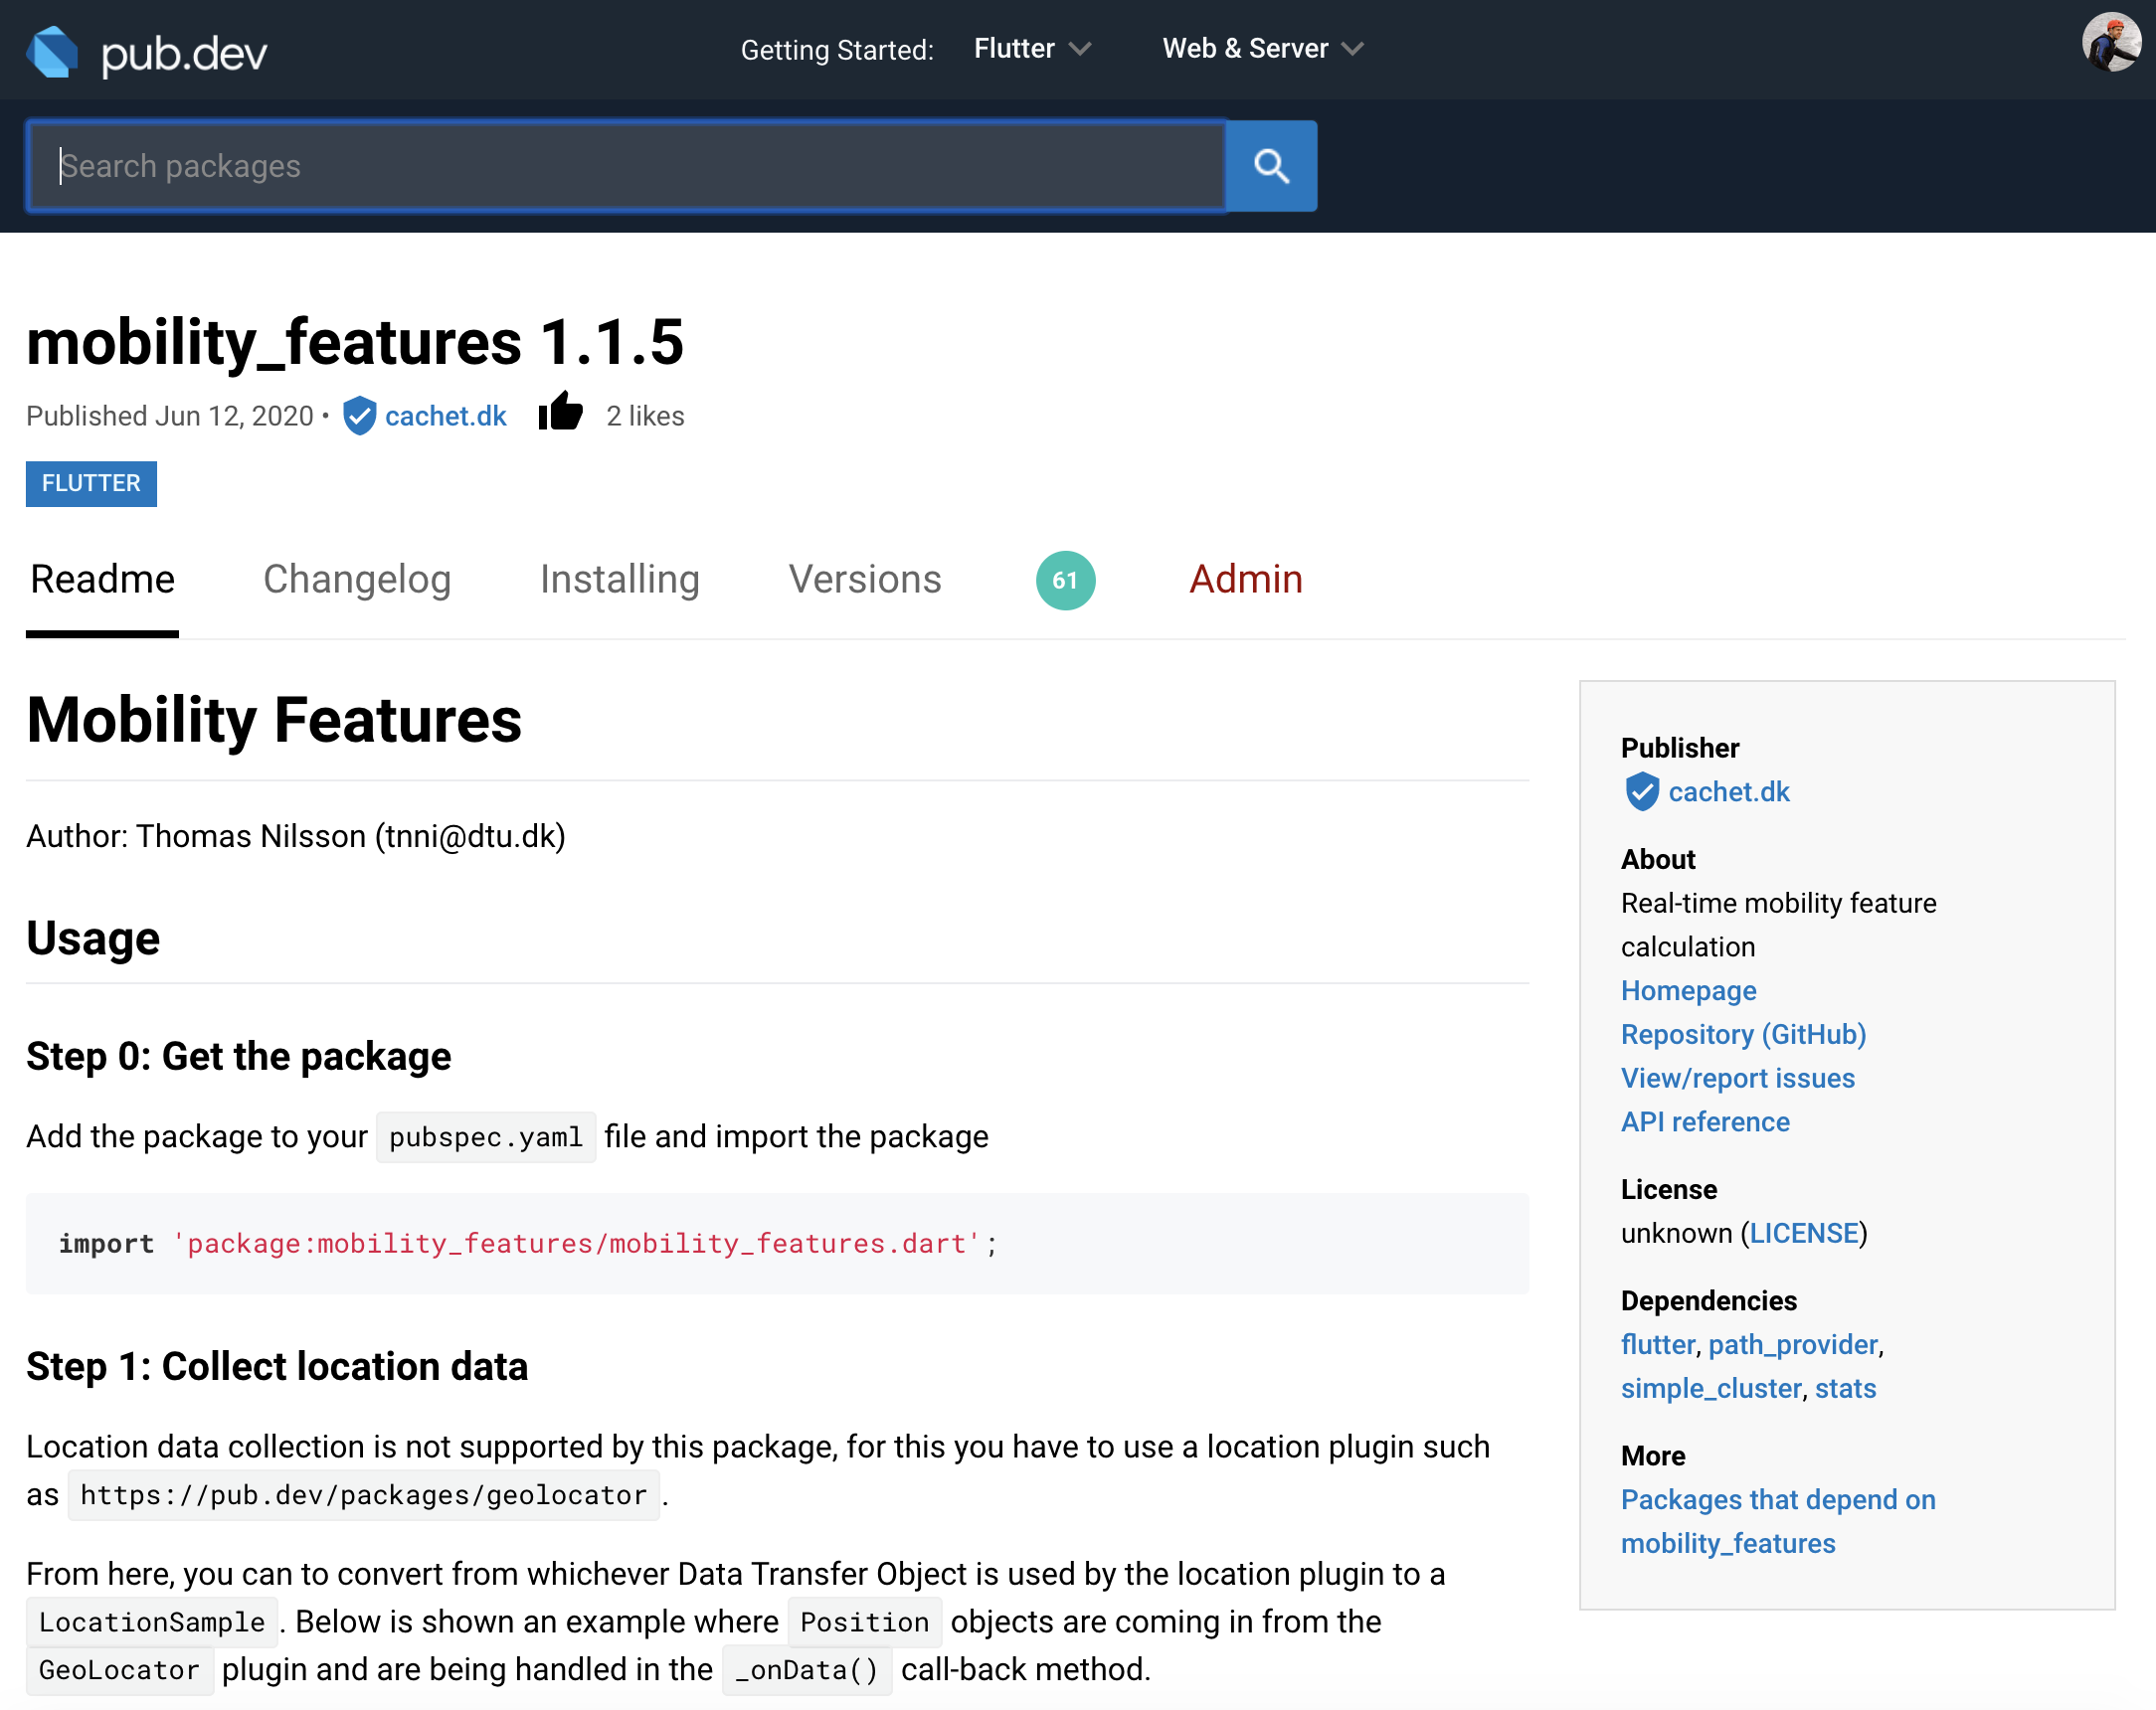
\includegraphics[width=\textwidth]{images/pub.png}
    \caption{The page hosting the Mobility Features Package on www.pub.dev}
    \label{fig:pub-package}
\end{figure}

Publishing automatically generate API documentation by using comments in the code. Normally, comments are made with 2 forward slashes (\textit{//}), but comments made with three forward slashes (\textit{///}) mark the code-block following it with API documentation, i.e. the contents of the comment. 

\begin{figure}
    \centering
    \begin{minted}{dart}
        /// A [LocationSample] holds a 2D [GeoPosition] spatial data point
        /// as well as a [DateTime] value s.t. it may be temporally ordered
        class LocationSample implements _Serializable, _Geospatial {...}
    \end{minted}
    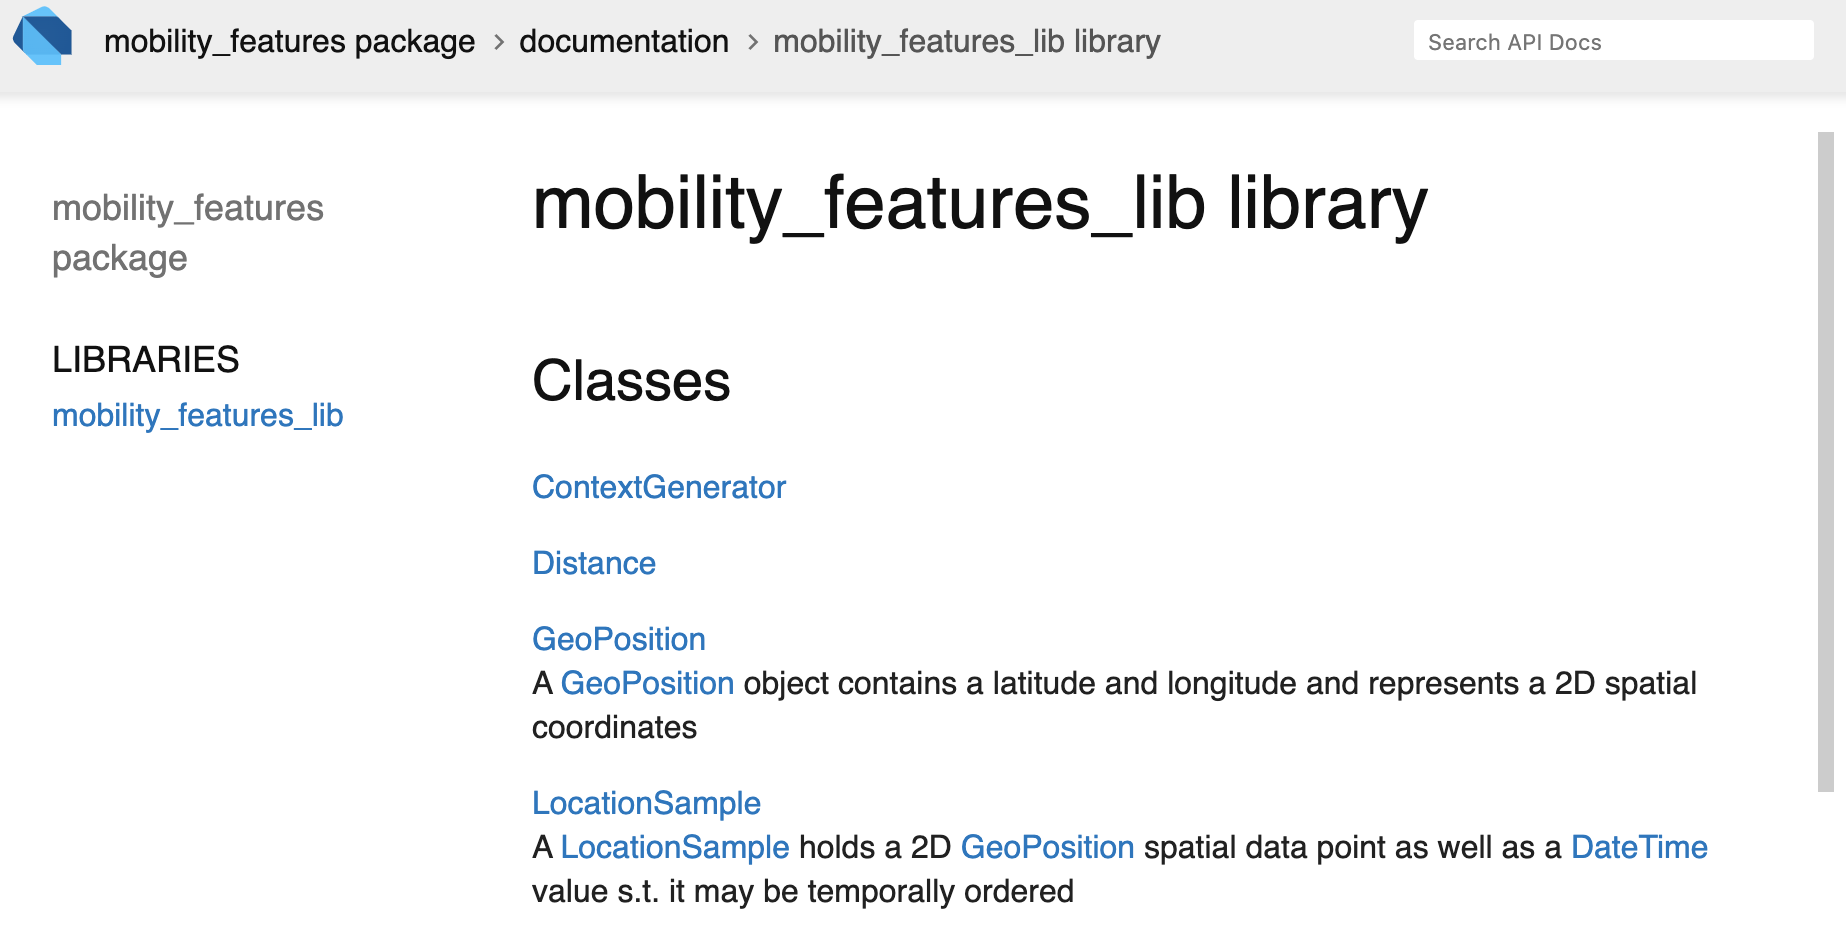
\includegraphics[width=\textwidth]{images/docs.png}
    \caption{The API comments for the source code of a Location Sample (top) and the auto generated documentation hosted on the Pub (bottom)}
    \label{fig:api-docs}
\end{figure}


\section{Package Implementation}
The package was implemented in Flutter according to the design in Chapter \ref{chapter:04} in which a series of components and the overall data model was outlined. This section will go through selected examples of source code as well as the general principles applied, to achieve the specified design, when implementing in Flutter and Dart.

\subsection{Private and Public Access}
In most objective oriented languages, such as Dart, the safest way to use fields in classes is to make them private, and to implement a parameter-less 'getter' method for retrieving the value, and a 'setter' method which takes in the new value as its parameter. In the Dart programming language, a field is declared private by having the the underscore prefix, i.e. \verb|routineIndex| becomes \verb|_routineIndex|, and the corresponding getter method is declared with \verb|get| and is simply called the \verb|routineIndex|:

\begin{minted}{dart}
class MobilityContext {

  double _routineIndex;
  ...
  double get routineIndex {
    return _routineIndex;
  }
}
\end{minted}

This results in an easy-to-read syntax when getting the value of the field, which looks like this:

\begin{minted}{dart}
MobilityContext c = MobilityContext(...);
print(c.routineIndex);
\end{minted}

The same concept can be applied to a constructor as well as the whole class. A public constructor is declared as:
\begin{minted}{dart}
GeoPosition(this._latitude, this._longitude);
\end{minted}

With the private equivalent being:

\begin{minted}{dart}
GeoPosition._(this._latitude, this._longitude);
\end{minted}

A private constructor allows the class to be publicly \textit{available} but not publicly \textit{instantiable}. For classes the underscore prefix is used for the class name, to make it private, similar to field, i.e. \verb|class HourMatrix| becomes \verb|class _HourMatrix|.

On the note of constructors, this package makes use of factory constructors which are effectively just methods which generate an object using the normal constructor. A factory constructor may be used to construct an object from JSON data, where each relevant field is extracted from the JSON data and passed onto the real constructor. A factory constructor is defined as follows:
\begin{minted}{dart}
factory Stop._fromLocationSamples(...) {
	return Stop._(...);
}
\end{minted}

\subsection{Domain Model Implementation}
All the components specified in the Domain Model Chapter \ref{chapter:04} were implemented with their repsective relations to each other. As specified in the component diagram \ref{fig:component-diagram} the only component with a public-facing constructor was LocationSample, and by transitivity, also GeoPosition. This is done, as mentioned, to allow the user instantiate a LocationSample with data from a given Location DTO. The GeoPosition class a field for the latitude and one for the longitude and a fundamental class used by the GeoSpatial interface. The interface is a private abstract class which means it is only visible internally in the package library.

\begin{minted}{dart}
abstract class _Geospatial {
  GeoPosition get geoPosition;
}
\end{minted}

This interface allows other classes to promise the Dart compiler that it has a GeoPosition field which allows it to be compared to other classes which implement the same interface. In Dart interfaces and abstract classes are one and the same thing, and the \textit{abstract class} keyword is used for implementing them. The GeoPosition class even implements this interface since a GeoPosition object itself has a GeoPosition. This may seem superfluous, but will come in handy when finding Stops.

\begin{minted}{dart}
class GeoPosition implements _Serializable, _Geospatial {
  double _latitude;
  double _longitude;

  GeoPosition(this._latitude, this._longitude);

  GeoPosition get geoPosition => this;
  double get latitude => _latitude;
  double get longitude => _longitude;
}
\end{minted}

\subsection{Storing and Loading Data}
The storing and loading of data, which includes Location Samples, Stops and Moves happen through the MobilitySerializer class. This class allows classes which implement the Serializable interface to be serialized and de-serialized. Just like the GeoSpatial interface, the Serializable interface is also implemented as a private abstract class only used internally in the package library. The interface contains a method for serializing a class to JSON, named \verb|toJson()| which takes no parameters and produces a HashMap of Strings to the dynamic, the dynamic type meaning any type. This is the Dart equivalent of a JSON object. Another method the interface forces other classes to implement is the deserialization method \verb|fromJson(json)| which takes a JSON object as parameter and creates a runtime object of the given type, from the JSON object. The implemention of this method is left to the individual classes implementing the interface which is done by extracting data from the JSON object.

\begin{minted}{dart}
abstract class _Serializable {
  Map<String, dynamic> _toJson();

  _Serializable._fromJson(Map<String, dynamic> json);
}
\end{minted}

The MobilitySerializer class is a generic which allows the type \verb|E| to be specified later, with \verb|E| referring to either an Location Sample, Stop or Move which all implement the Serializable interface. The MobilitySerializer is constructed using a reference to a File object. The File object is used for storing the data of the given type i.e. Location Samples are stored one file, Stops in another and Moves in a third.

\begin{minted}{dart}
class MobilitySerializer<E> {
  File file;
  
  MobilitySerializer._(this.file) {
    bool exists = file.existsSync();
    if (!exists) {
      flush();
    }
  }
  
  Future<void> flush() async =>
      await file.writeAsString('', mode: FileMode.write);
\end{minted}

When initialized, it is checked whether or not the specified file exists, and if not the \verb|flush| method is called, which simply writes an empty string to the file, overriding any content, which has the effect of creating the file, should it not already exist. A concrete example of instantiated the MobilitySerializer for Stops is shown below, where \textit{stops.json} refers to the file in which Stops should be stored.

\begin{minted}{dart}
MobilitySerializer<Stop> stopSerializer =
        MobilitySerializer<Stop>._(await _file('stops.json'));
\end{minted}

For storing data the \verb|save| method is used which takes in a list of objects which all implement the Serializable interface. Each element in the list is serialized via its \verb|toJson| method and concatenated into one big string separated by a delimiter token, and this string is then written to the specific file of the MobilitySerializer object.

\begin{minted}{dart}
Future<void> save(List<_Serializable> elements) async {
  String jsonString = "";
  for (_Serializable e in elements) {
    jsonString += json.encode(e._toJson()) + delimiter;
  }
  await file.writeAsString(jsonString, mode: FileMode.writeOnlyAppend);
}
\end{minted}

Loading works in the reverse order, where the contents of the specified file is loaded into a string, the string is then split into elements using the delimiter token and each of these elements is turn de-serialized using the \verb|fromJson| method.  For deciding which type to de-serialize the elements into, a switch statement is used that checks the type of \verb|E| which is specified when the MobilitySerializer object is instantiated.

\begin{minted}{dart}
Future<List<_Serializable>> load() async {
    String content = await file.readAsString();

    List<String> lines = content.split(delimiter);

    Iterable<Map<String, dynamic>> jsonObjs = lines
        .sublist(0, lines.length - 1)
        .map((e) => json.decode(e))
        .map((e) => Map<String, dynamic>.from(e));

    switch (E) {
      case Move:

        return jsonObjs.map((x) => Move._fromJson(x)).toList();
      case Stop:

        return jsonObjs.map((x) => Stop._fromJson(x)).toList();
      default:

        return jsonObjs.map((x) => LocationSample._fromJson(x)).toList();
    }
  }
\end{minted}

Ideally, the switch statement could have been replaced by the following one-liner:
\begin{minted}{dart}
return jsonObjs.map((x) => E.fromJson(x)).toList();
\end{minted}

However, this relies on the language feature called reflection \footnote{\url{https://www.javaworld.com/article/2075801/reflection-vs--code-generation.html}} which allows the compiler to infer the type of \verb|E| at compile-time. However, Dart does not support \textit{reflection} which makes this impossible.

\subsection{Finding Intermediate Features}
Finding the intermediate features Stops, Moves and Places were done according to the algorithms described in Chapter \ref{chapter:03}. 

\subsubsection{Finding Stops}
The Stop class has two constructors: A factory constructor which takes a set of LocationSamples from which the centroid of the set is computed, as well as the earliest timestamp, which will be the arrival time, and the latest timestamp which will be the departure time. After these attributes are found, the normal constructor is used.

\begin{minted}{dart}
  factory Stop._fromLocationSamples(List<LocationSample> locationSamples,
      {int placeId = -1}) {
      
    GeoPosition center = _computeCentroid(locationSamples);
    return Stop._(center, locationSamples.first.datetime, locationSamples.last.datetime,
        placeId: placeId);
  }
\end{minted}

The normal constructor uses a GeoPosition, in addition to an arrival and departure time. A place ID may also be specified at construction, but often it is not yet known at construction time hence it is optional.

\begin{minted}{dart}
  Stop._(this._geoPosition, this._arrival, this._departure, {this.placeId = -1});
\end{minted}

The Stop algorithm takes a List of LocationSamples as input, and uses two while-loops, and two pointers (\textit{start} and \textit{end}) which delimit a subset of the input data we are currently considering with the outer loop. Every time the outer loop moves, the \textit{start} pointer is moved past the end pointer, in order to skip already seen data. The inner loop is responsible for moving the \textit{end} pointer: With each iteration of the inner loop, the centroid of the current subset is computed. If the distance from this centroid to the latest added sample is within the given \verb|stopRadius| parameter, then the subset is expanded by incrementing the \textit{end} pointer., and the process is continued. Otherwise the inner loop terminates and a Stop is created from the subset. The Stop is created without a Place ID, since Places have not yet been identified. In addition, Stops with a duration shorter than the duration specified by the \verb|stopDuration| parameter are removed since they are noisy. This is an addition to the algorithms previously described and is mostly used due to the very high sampling frequency and likely won't be necessary in the general case.

\begin{minted}{dart}
  int start = 0;
  while (start < n) {
    int end = start + 1;
    List<LocationSample> subset = data.sublist(start, end);
    GeoPosition centroid = _computeCentroid(subset);

    while (
        end < n && Distance.fromGeospatial(centroid, data[end]) <= stopRadius) {
      end += 1;
      subset = data.sublist(start, end);
      centroid = _computeCentroid(subset);
    }
    Stop s = Stop._fromLocationSamples(subset);
    stops.add(s);

    start = end;
  }
\end{minted}

The distance calculation \verb|Distance.fromGeospatial(centroid, data[end]) <= stopRadius)| is carried out using the \verb|GeoSpatial| interface previously mentioned. The distance function \verb|fromGeoSpatial| takes two objects which implement the interface and unpacks the latitude and longitude from these objects. The haversine distance can then be computed afterwards.

\begin{minted}{dart}
class Distance {
  static double fromGeospatial(_Geospatial a, _Geospatial b) {
    return fromList(
        [a.geoPosition._latitude, a.geoPosition._longitude],
        [b.geoPosition._latitude, b.geoPosition._longitude]);
  }

  static double fromList(List<double> p1, List<double> p2) {
    /// Haversine implementation
  }
}
\end{minted}

\subsubsection{Finding Moves}
The Move class has two constructors which are both private. Common for both constructors is that they take two Stops as arguments, with argument being either a path of Locaiton Samples or a Distance, i.e. a double. The factory constructor called \verb|_fromPath| calculates the distance of the path and then uses the normal constructor for create a Move. 
\begin{minted}{dart}
  factory Move._fromPath(Stop a, Stop b, List<LocationSample> path) {
    double d = _computePathDistance(path);
    return Move._(a, b, d);
  }
\end{minted}

\begin{minted}{dart}
  Move._(this._stopFrom, this._stopTo, this._distance);
\end{minted}
The normal constructor is used for de-serialization whereas the factory constructor is used to create a Move given two Stops and the path of samples between them.

The algorithm for finding Moves takes a List of Location Samples and the Stops found from the samples as input. The algorithm first checks if the set of Stops is empty, and if so returns an empty set of Moves. If however the set of Stops is not empty, then two 'fake' Stops are created and added to the set of Stops. These two additional stops are created from the first and last element in the set of Location Samples. For each Stop in the set of Stops, it is calculated which samples lie in between the current and next Stop. A Move is then created using the current Stop, the next Stop and the path between. 

\begin{minted}{dart}
  Stop first = Stop._fromLocationSamples([data.first]);
  List<Stop> allStops = [first] + stops;

  if (data.first != data.last) {
    Stop last = Stop._fromLocationSamples([data.last]);
    allStops.add(last);
  }

  for (int i = 0; i < allStops.length - 1; i++) {
    Stop cur = allStops[i];
    Stop next = allStops[i + 1];
    List<LocationSample> samplesInBetween = data
        .where((d) =>
            cur.departure.leq(d.datetime) && d.datetime.leq(next.arrival))
        .toList();

    moves.add(Move._fromPath(cur, next, samplesInBetween));
  }
\end{minted}

The mentioned 'fake' Stops is an addition to the definition in Chapter \ref{chapter:03}. They are created to avoid situations in which tracking was started while moving, in this case no Moves are created before the user is stationary for some time, and Stops are found. This situation will likely not be very common, but was found during self-study and therefore deemed worthy of covering. The extra Stops are only used for finding moves and will not be used for finding Places.

\subsubsection{Finding Places}
The Place class only has one normal constructor which takes an ID (an integer) and a List of Stops. 
\begin{minted}{dart}
Place._(this._id, this._stops);
\end{minted}

The Place algorithm takes a set of Stops for a given period, i.e. Stops over multiple days. The DBSCAN algorithm \cite{density-based-1996} is used to find clusters in the Stops and label each Stop with a cluster ID, this is the place ID previously discussed. Once the labels are computed the Stops are grouped by their Place ID, and a for each group a Place object is created with the group label and the Stops contained in the group. Lastly, the \verb|placeId| attribute for each Stop in the group is set to the group label.

\begin{minted}{dart}
  DBSCAN dbscan = DBSCAN(
      epsilon: placeRadius, minPoints: 1, distanceMeasure: Distance.fromList);
  List<List<double>> stopCoordinates =
      stops.map((s) => ([s.geoPosition.latitude, s.geoPosition.longitude])).toList();

  dbscan.run(stopCoordinates);

  Set<int> clusterLabels = dbscan.label.where((l) => (l != -1)).toSet();

  for (int label in clusterLabels) {
    List<int> indices =
        stops.asMap().keys.where((i) => (dbscan.label[i] == label)).toList();

    List<Stop> stopsForPlace = indices.map((i) => (stops[i])).toList();

    Place p = Place._(label, stopsForPlace);
    places.add(p);

    stopsForPlace.forEach((s) => s.placeId = p._id);
  }
\end{minted}

\subsection{Comuting Features}
A Mobility Context object represents features for a given date. The class has private constructor which takes a List of Stops and Moves from today, and a List of Places from the current period, i.e. the last 28 days including today. When the class is instantiated the date of today is automatically inferred, if not provided through the date parameter, which is an optional parameter. This parameter can be overridden in the case of unit testing for specific dates or if the programmer wishes to compute a Mobility Context for a date in the past.

\begin{minted}{dart}
MobilityContext._(this._stops, this._allPlaces, this._moves,
  {this.contexts, this.date}) {
  _timestamp = DateTime.now();
  date = date ?? _timestamp.midnight;
}
\end{minted}

The other optional parameters is a List of Mobility Contexts is used for computing the Routine Index - how this is achieved will be explained later in this section. The 'derived' features are implemented as doubles (except for Number of Places which is an integer) and are fields in the Mobility Context class. All of these features are accessed via getters, which retrieve the value of the field.

\begin{figure}
    \centering
    \begin{minted}{dart}
    class MobilityContext {
    	// Field
    	double _routineIndex;
     
     	// Getter
        double get routineIndex {
        	return _routineIndex;
        }
    }
    \end{minted}
    \caption{The getter method for a feature field}
    \label{fig:feature-getter}
\end{figure}

\subsubsection{Lazy Evaluation}
A \textit{getter} method for a given feature should reflect that the feature that is to be retrieved requires minimal computation (i.e. 'getting'), and therefore the feature computation should not take place in the getter method. However there is a middle way, since the given feature needs to be computed only once to be evaluated, which allows us to keep the getter syntax. This middle way is \textit{lazy evaluation} \footnote{\url{https://www.martinfowler.com/eaaCatalog/lazyLoad.html}}, which is the idea of having a field be computed only the first time it is needed, and then stored from then on. In practice this is done by letting the field be initialized to \textit{null}, and checking for \textit{null} in the getter method. If the value is \textit{null} then the feature is calculated and the field's value is updated after the computation and the getter can return the field's value. If the field is not \textit{null} then the feature has already been computed, and can be returned immediately.

\begin{figure}
    \centering
    \begin{minted}{dart}
    class MobilityContext {
        // Field
        double _routineIndex;
        
        // Getter
        double get routineIndex {
            if (_routineIndex == null) {
                _routineIndex = _calculateRoutineIndex();
            }
            return _routineIndex;
        }
    }
    \end{minted}
    \caption{Lazy evaluation of a feature}
    \label{fig:lazy-evaluation}
\end{figure}


\subsubsection{Home Stay Computation}
The derived features are computed according to their definitions in \ref{chapter:03}, using the lazy evaluation template outlined in Figure \ref{fig:lazy-evaluation}. The Home Stay feature is not exception. The algorithm for computing Home Stay uses the Stops of today: First, the total time elapsed today is calculated using the departure timestamp of the last known Stop of today. Next, the Stops are used to identify the home place by constructing an Hour Matrix, and then extracting the \verb|homePlaceId| from the Hour Matrix. Then, the total duration spent at the home Place is calculated by summing the duration of the Stops which belong to the home Place. The Home Stay is then calculated as the time at home divided by the total time elapsed.

\begin{figure}
    \centering
\begin{minted}{dart}
double _calculateHomeStay() {
  // Latest known sample time
  DateTime latestTime = _stops.last.departure;

  // Total time elapsed from midnight until the last stop
  int totalTime = latestTime.millisecondsSinceEpoch -
      latestTime.midnight.millisecondsSinceEpoch;

  // Find todays home id, if no home exists today return -1.0
  _HourMatrix hm = this.hourMatrix;
  if (hm.homePlaceId == -1) {
    return -1.0;
  }

  int homeTime = stops
      .where((s) => s.placeId == hm.homePlaceId)
      .map((s) => s.duration.inMilliseconds)
      .fold(0, (a, b) => a + b);

  return homeTime.toDouble() / totalTime.toDouble();
}
\end{minted}
    \caption{The method for computing the Home Stay feature}
    \label{fig:home-stay-code}
\end{figure}

\subsubsection{Routine Index}
The Routine Index is the most difficult to compute by far. The method for computing this feature inside the Mobility Context class is however quite short, but this is due to all the matrix computations being done in the Hour Matrix class, i.e. the averaging and overlapping of matrices. The algorithm first checks if any contexts are provided if not then the Routine Index should be -1.0. Next, the Hour Matrices for each historic date is computed, and from these the average Hour Matrix is computed. Lastly the Routine Index is found by computing the overlap between the two Hour Matrix of today, and the average Hour Matrix, using the \verb|a.computeOverlap(b)| method of the Hour Matrix class.

\begin{figure}
    \centering
    \begin{minted}{dart}
    double _calculateRoutineIndex() {
      // Require at least 2 days to compute the routine index
      if (contexts == null) {
        return -1.0;
      } else if (contexts.isEmpty) {
        return -1.0;
      }
    
      /// Compute the HourMatrix for each context that is older
      List<_HourMatrix> matrices = contexts
          .where((c) => c.date.isBefore(this.date))
          .map((c) => c.hourMatrix)
          .toList();
    
      /// Compute the 'average day' from the matrices
      _HourMatrix avgMatrix = _HourMatrix.average(matrices);
    
      /// Compute the overlap between the 'average day' and today
      return this.hourMatrix.computeOverlap(avgMatrix);
    }
    \end{minted}
    \caption{The method for computing the Routine Index feature}
    \label{fig:routine-index-code}
\end{figure}


\subsection{Using Historical Data}
Historical  Store collected samples
Load collected samples
Filter collected samples
Data from day $n$ is deleted on day $n+1$ when loading

Load historical stops and moves
Filter stops and moves
Recompute for today, replace with new 
Append the filtered historical with new stops and moves
Store by overwriting existing stops and moves

\subsection{Context Generation}
Context Generator
Static class, does not have a state
References the LocationSample serializer, gives access to the user
Works as interface for computing things without being able to alter the state
Does the computation process
Async, since files need to be stored and loaded
Routine Index



\subsection{Improvements}
Currently the implementation (not the design) requires daily computation
If features are not computed on a given day, then all the data collected on that day will be lost next time features are computed due to being filtered out. Currently the user can avoid this by either computing features every day without fault or specifying the date on which the features are yet to be computed.
The fix is to mark data and not throw it out before stops and moves have been evaluated for those samples
When data is loaded, group by date, and compute stops and moves per date. Only then should the samples be thrown out.

Lazy evaluation should probably not be used, instead compute on initialization since initialization is async

ContextGeneration should be done with an isolate, currently the user needs to use an isolate.
Prevent UI thread from freezingMobilitySerializvi
\section{Using the Package}
This section will be a mirror of the official instructions on how to use the package, as of version \textit{1.2.0}. For getting started, the programmer has to download the package by adding it as a dependency in their \verb|pubspec.yaml| file of the Flutter project and running the following command:

\begin{minted}{sh}
flutter packages get
\end{minted}

Once the dependency has been downloaded it can be imported as follows:

\begin{minted}{dart}
import 'package:mobility_features/mobility_features.dart';
\end{minted}

Features are computed using the 3 lines of code displayed in Figure \ref{fig:code-example-intro}:

\begin{figure}[h]
    \centering
    \begin{minted}{dart}
    /// Collect data with a location plugin
    List<LocationSample> locationSamples = ///

    /// Store data via the package
    await ContextGenerator.saveSamples(locationSamples);
    
    /// Compute Features via the package
    MobilityContext context = await ContextGenerator.generate();
    \end{minted}
    \caption{All the three lines of code necessary for the application developer to write}
    \label{fig:code-example-intro}
\end{figure}

The exact method for arriving at this stage is outlined in the following 4 steps.

\subsection*{Step 1: Collect location data}
Location data collection is, as mentioned, not part of the Mobility Features package. The location plugin can be flexibly chosen by the programmer. An example of such a plugin the \textit{GeoLocator} plugin\footnote{\url{https://pub.dev/packages/geolocator}}. From here, each incoming location object has to be converted to a \verb|LocationSample| via the constructor

Below is shown an example where incoming \verb|Position| objects are coming in from the \textit{GeoLocator} plugin and are being handled after saved to a list, in the \verb|_onData()| call-back method.

\begin{minted}{dart}
List<LocationSample> locationSamples = [];
...

void _onData(Position d) async {
    GeoPosition geoPos = GeoPosition(d.latitude, d.longitude);
    LocationSample sample = LocationSample(geoPos, d.timestamp);
    locationSamples.add(sample);
}
\end{minted}

\subsubsection*{Step 2: Save location data}
The location data must be saved on the device such that it can be used in the future. Saving the data to persistent storage prevents it from being lost should the RAM reset. Given that the programmer has collected the samples in a list, the samples can be serialized using the \verb|save()| method of the MobilitySerializer.

\begin{minted}{dart}
await ContextGenerator.saveSamples(locationSamples)
\end{minted}

Ideally, saving the data is done with a certain interval, such as every time 100 samples are collected. 

\subsection*{Step 3: Compute features}
The Features can be computed using the static class \verb|ContextGenerator| which uses the stored location samples, as well as historic features to compute the features for today.

There most basic computation is done as follows:
\begin{minted}{dart}
MobilityContext context = await ContextGenerator.generate();
\end{minted}

Note: it is not possible to instantiate a MobilityContext object directly. 
It must be instantiated through \verb|ContextGenerator.generate()|.

\subsubsection*{Step 3.1: Compute features with prior contexts}
Should the programmer wish to compute the routine index feature as well, then prior contexts are needed. Concretely, the application needs to have tracked data for at least 2 days, to compute this feature. The generation of a Mobility Context using prior contexts is done by overriding the \verb|usePriorContexts| argument and setting it to \verb|true|.

\begin{minted}{dart}
MobilityContext context = 
    await ContextGenerator.generate(usePriorContexts: true);
\end{minted}

\subsubsection*{Step 3.2: Compute features for a specific date}
By default, a MobilityContextobject uses the current date as a reference to filter and group data, however, should one wish to compute the features for a specific date, then it is possible to do so by overriding the \verb|today| argument and providing the desired date.

\begin{minted}{dart}
DateTime myDate = DateTime(01, 01, 2020);
MobilityContext context = 
    await ContextGenerator.generate(today: myDate);
\end{minted}

\subsection*{Step 4: Get features}
All features are implemented as \textit{getters} for the MobilityContext class and can, therefore, be retrieved using the dot-notation. 

\begin{minted}{dart}
MobilityContext context = // Generate context

List<Place> places = context.places;
List<Stop> stops = context.stops;
List<Move> moves = context.moves;

int numberOfPlaces = context.numberOfPlaces;
double homeStay = context.homeStay;
double entropy = context.entropy;
double normalizedEntropy = context.normalizedEntropy;
double distanceTravelled = context.distanceTravelled;
double routineIndex = context.routineIndex;
\end{minted}




\chapter{Validation}
\label{chapter:06}
To validate the Mobility Features Package in a real world setting, a small-scale field study was conducted in which 10 participants were tracked over 3 weeks. For this study a mobile application was developed in Flutter that used the package to compute features on a daily basis. Subjective user-data also collected through the application in the form of a small questionnaire. This chapter will go through the choices made in developing the app and conducting the study.

\section{Field Study}
A small-scale study similar to that of Cuttone et al. \cite{sparse-location-2014} was conducted which ran for 3 weeks and included 10 participants (including the author). The goal of the study was to validate the accuracy of the features produced. In the study the participants used the application discussed in Chapter \ref{chapter:05} to collect their location data and computed mobility features daily. In addition, participants answered a questionnaire daily to get subjective user data. 

\subsection{Self-study}
Before the main study was conducted a self-study was conducted in three different cities, in order to select appropriate parameters for the algorithms. This parameter tweaking happened while the author was in Munich where he sat in a large university building and visited different offices. In Figure \ref{fig:tum-map} the Places and the Stops at the university are displayed and as can be seen which are very close. Had the radius parameter for finding places been higher, then some of the found places would have been merged into a single place. Here, the parameter was set to 25 meters, and in the final study, it was chosen to set it to 50 meters.

\begin{figure}
    \centering
    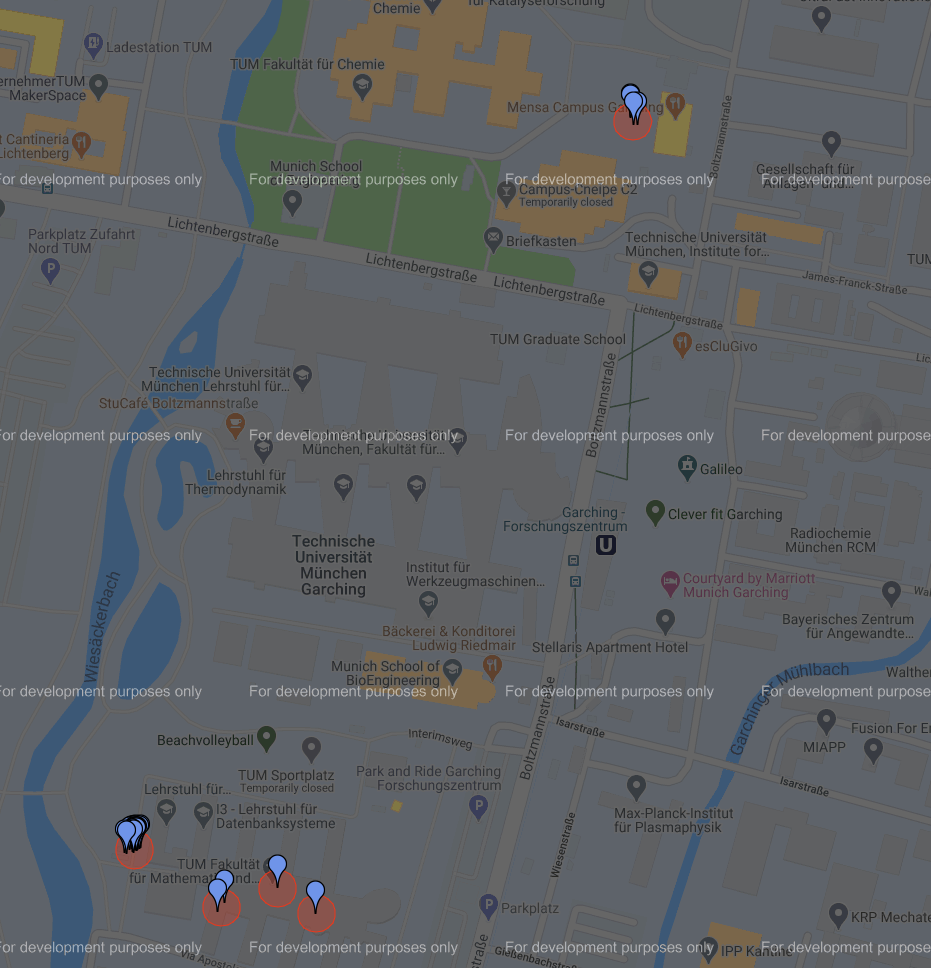
\includegraphics[width=0.7\textwidth]{images/map/map-tum.png}
    \caption{A map of TUM Garching, displaying the Places (red clusters) as well as the Stops which make up these places (blue markers) visited by the author}
    \label{fig:tum-map}
\end{figure}

\subsection{Main Study}
In addition to this, the application also had a diary consisting of 4 questions that the participant had to fill out each day. In order to make it easy for the user to remember filling out the diary, a reminder was sent to the participants at 8 PM. The time 8 PM was chosen due to being relatively late while still being early enough in the day that people would still be checking their phone. Some people go to bed at 9-10 PM which had to be taken into account. The diary questions were related to 3 of the Mobility Features which were \textit{Number of Clusters}, \textit{Home Stay} and \textit{Routine Index}. The purpose of the questions was to get subjective estimates of the values of these features. It is important to stress that answers are very rounded off, since the participants cannot be expected to give very precise answers. Answers are also highly subjective since the definition of things such as a 'place' may vary a lot from person to person.

\subsection{Evaluating Features}
Answers were collected through a diary in order to evaluate the accuracy of the computed features. The features inquired about had to be easy to formulate as a question such that participants could provide reliable answers. Features such as entropy and location variance were ill-suited for this, whereas Home Stay, Number of Places, and Routine Index were chosen instead. The questions were the following:

\begin{itemize}
    \item[\#1] How many unique places (including home) did you stay at today?
    \item[\#2] How many hours did you spend away from home today? (Rounded-up)
    \item[\#3] Did you spend time at places today that you don't normally visit?
    \item[\#4] On a scale of 0-5, how much did today look like the previous, recent days? (Where 0 means 'not at all' little and 5 means 'Exactly the same')
\end{itemize}

Collecting the subjective \textit{Number of Places} visited, was done by asking the participant how many places they had visited today, including their home. Technically it is possible that a user visits no places at all, but highly unlikely.\\

For collecting the subjective \textit{Home Stay} percentage, the participant was asked the inverse question, i.e. how many hours they were \textit{away} from their home today (from which Home Stay can then be calculated later). This question is much easier for the participant to answer, and there is no need to explain to the participant that time spent during the night counts towards the Home Stay, as an example. \\

The Routine Index was more difficult to formulate as a question since there is no succinct way of putting it. It was decided upon rating today scale from 0 to 5, where 0 indicates that today looks nothing like previous days and 5 indicating that today looks identical to the previous days. Ideally, the scale should be more fine-grained such as a 0 to 10 scale, however, this would put too much on the participant. The information we wished to know was, on a high level, whether or not today looked like the previous days which is still possible with a more coarse grained scale. Question \#3 also related to the Routine Index feature but was not used for later data analysis since it was hard to compare directly to the Routine Index and would require looking at the Hour Matrix instead.

\subsection{Hindrances}
The Coronavirus pandemic leads to countries closing borders and urging people to stay at home as much as possible. This included workplaces shutting down and people had to work from home, as well as places of recreational character such as gyms and restaurants. This had some implications for the study in that people would spend most of their time at home, and they would likely not visit very many places. In addition, it was probably also not common for most people to go visit new places during the pandemic. However, all in all, the pandemic only shaped the results of the field study and did not prevent the study from taking place at all. In addition the Android platform also closed down the access needed for tracking location data in the background without interruption as of February 2020 \footnote{\url{https://nakedsecurity.sophos.com/2020/02/25/android-11-to-clamp-down-on-background-location-access/}}\footnote{\url{https://developer.android.com/training/location/background}}. It was therefore chosen to focus on releasing and testing the application for iOS only, due to time constraints.



\section{Study Application}

\subsection{Installing the Application}
The application was only released on iOS as previously mentioned and therefore was distributed exclusively via the Apple App Store. When beta testing iOS applications one can use the TestFlight service provided by Apple which in its essence functions a separate App Store for applications in development, which require an invitation to install. Once the user had such an invitation the installation process was the following: The user installs the TestFlight application via the App Store, then opens the TestFlight application to find the Mobility Study app ready for installation. Once the Mobility Study app is installed, it will ask for permission to track the user's location as well as sending the user notifications. The location tracking is obviously necessary for the collection of location data, the notifications are not necessary but helps the user be reminded to fill out a daily questionnaire. An installation manual (see Appendix \ref{appendix:installation} was provided to the participants to ensure the applications were set up correctly.

\begin{figure}
    \centering
    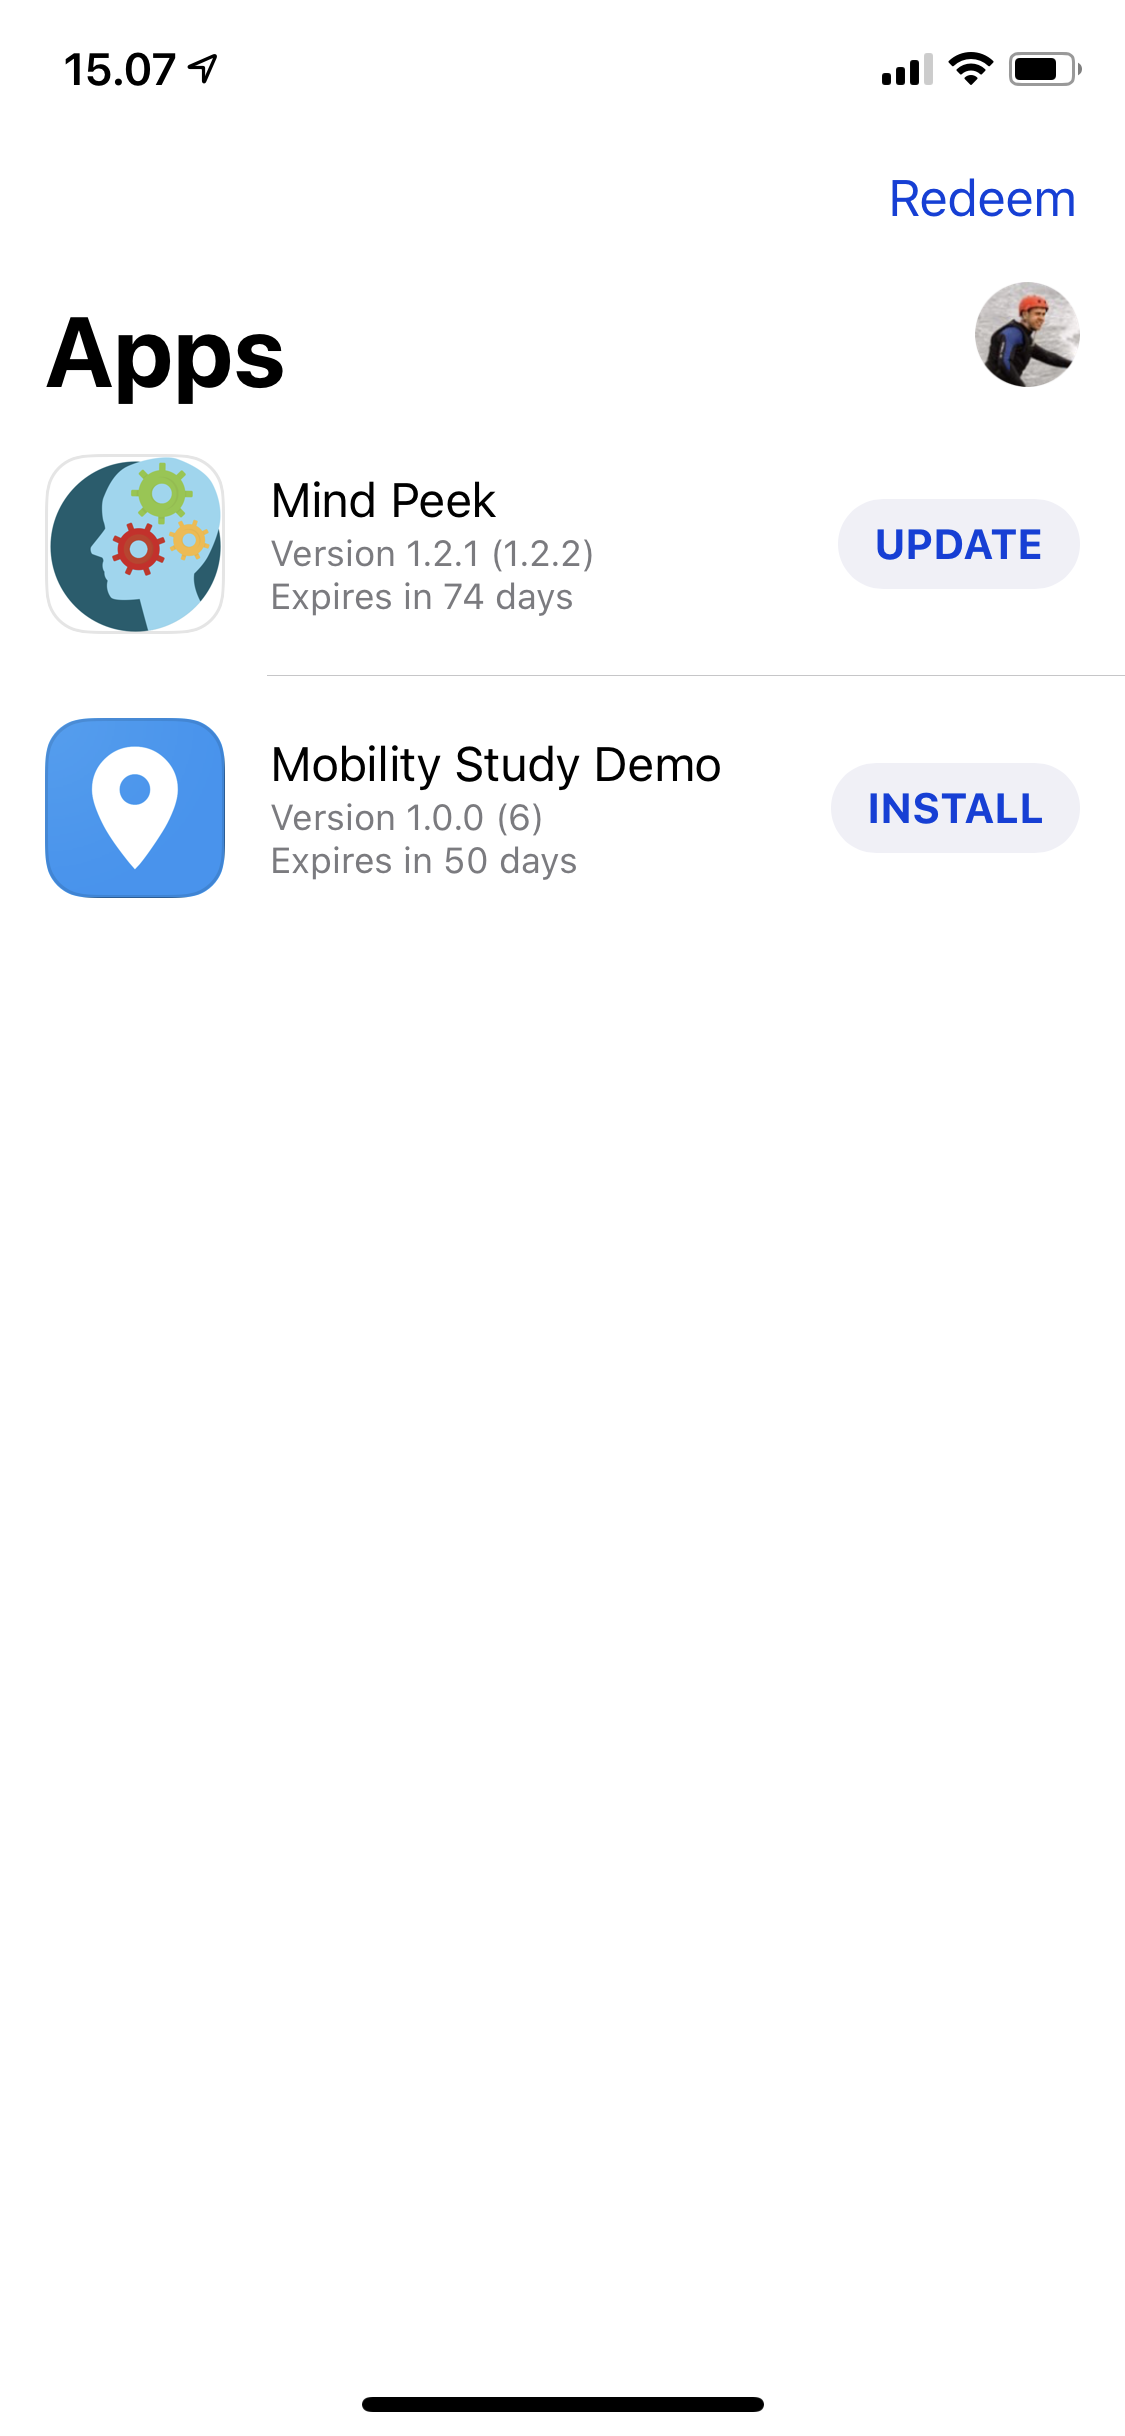
\includegraphics[width=0.2\textwidth]{images/app_imgs/app_testflight.png} 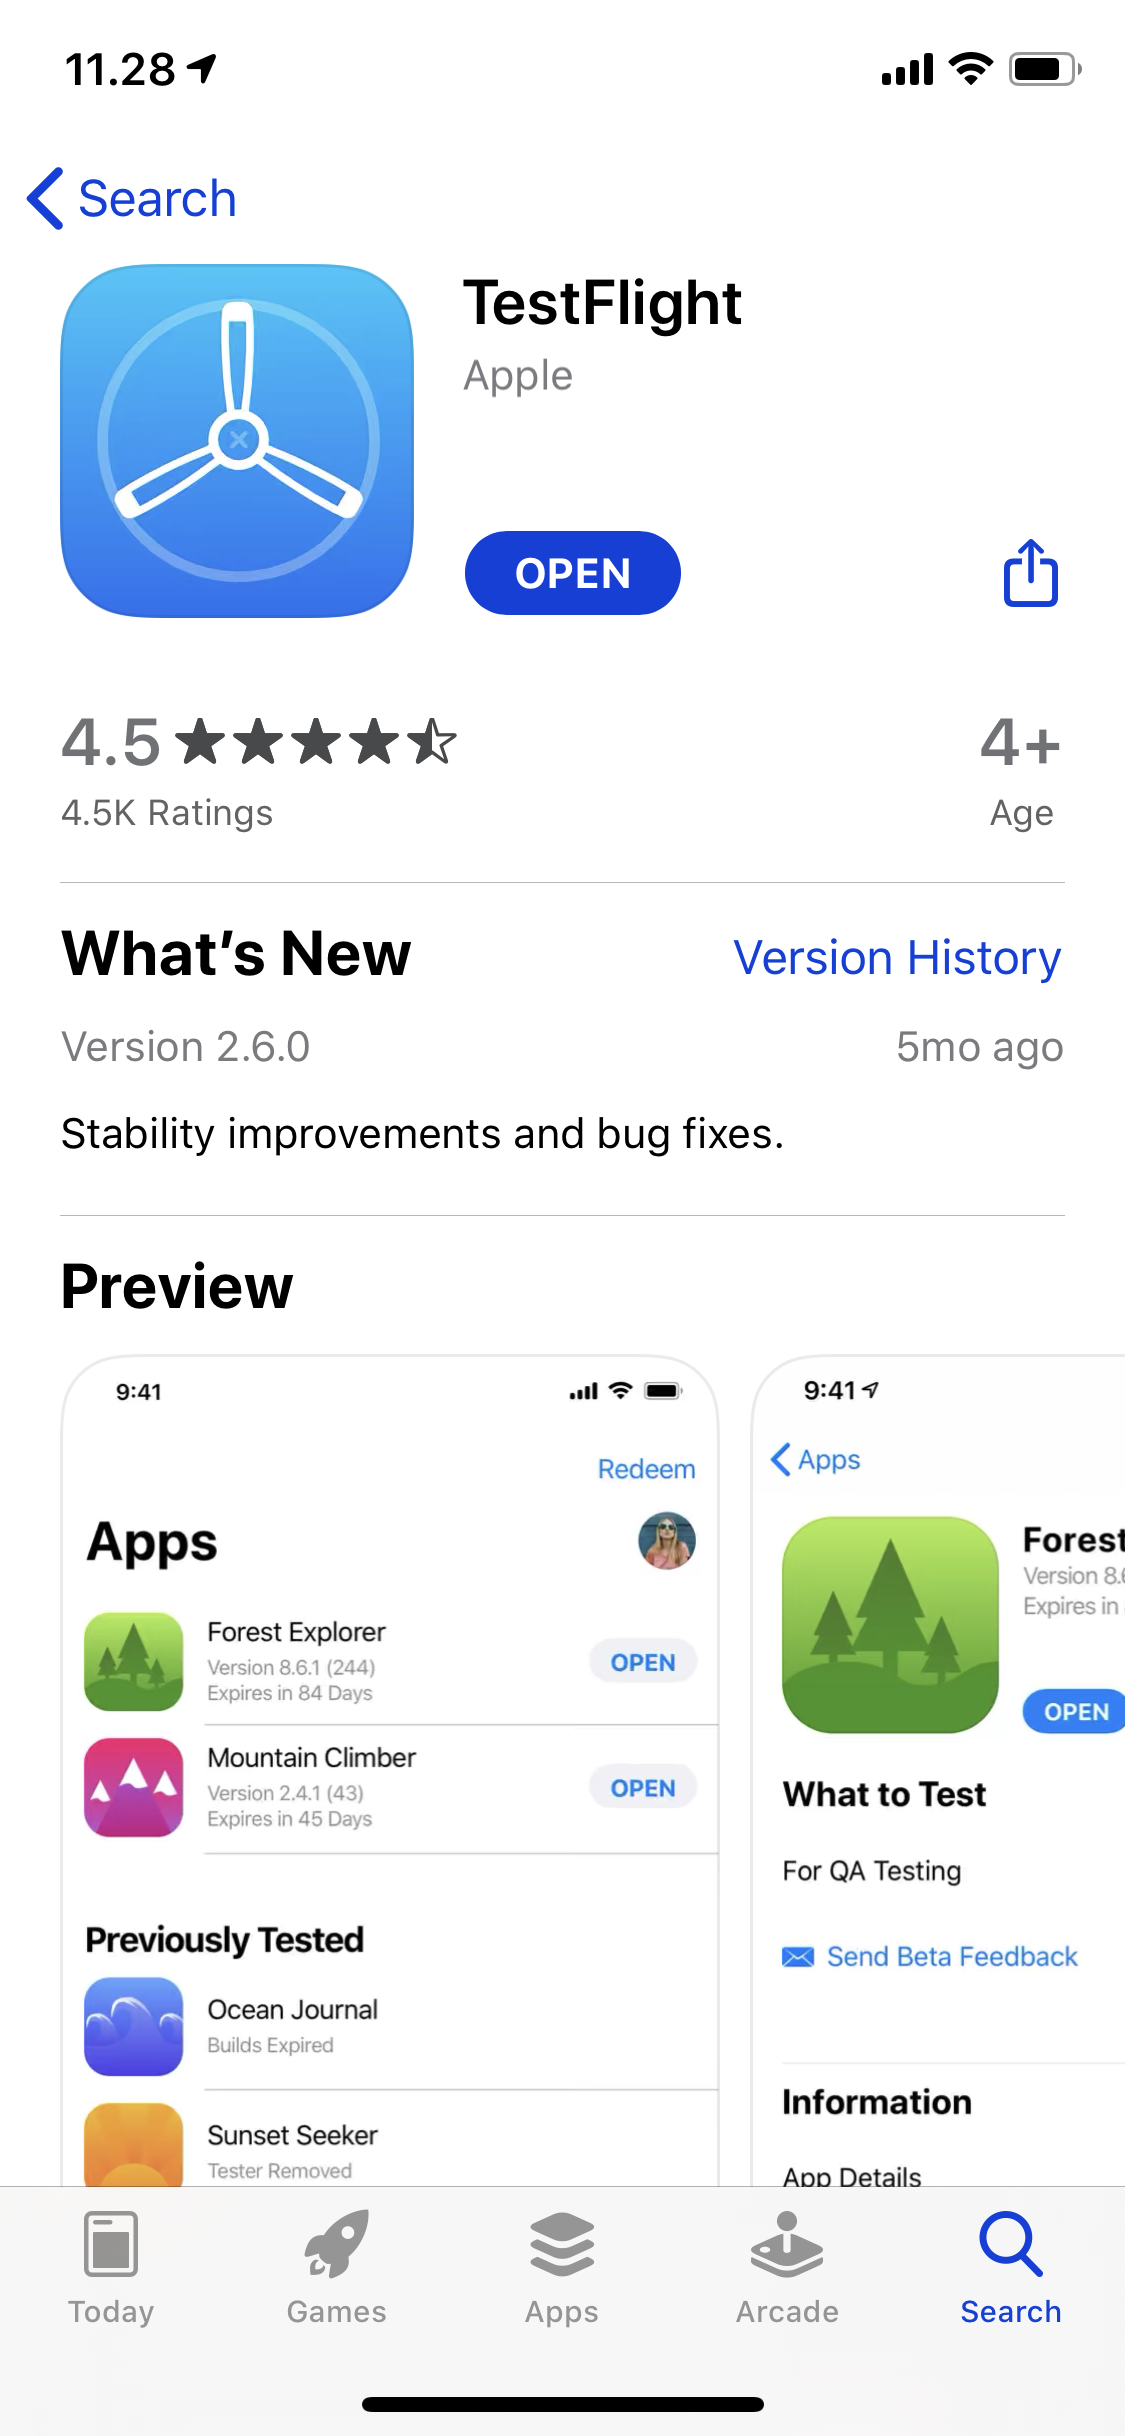
\includegraphics[width=0.2\textwidth]{images/app_imgs/app-appstore.png}
    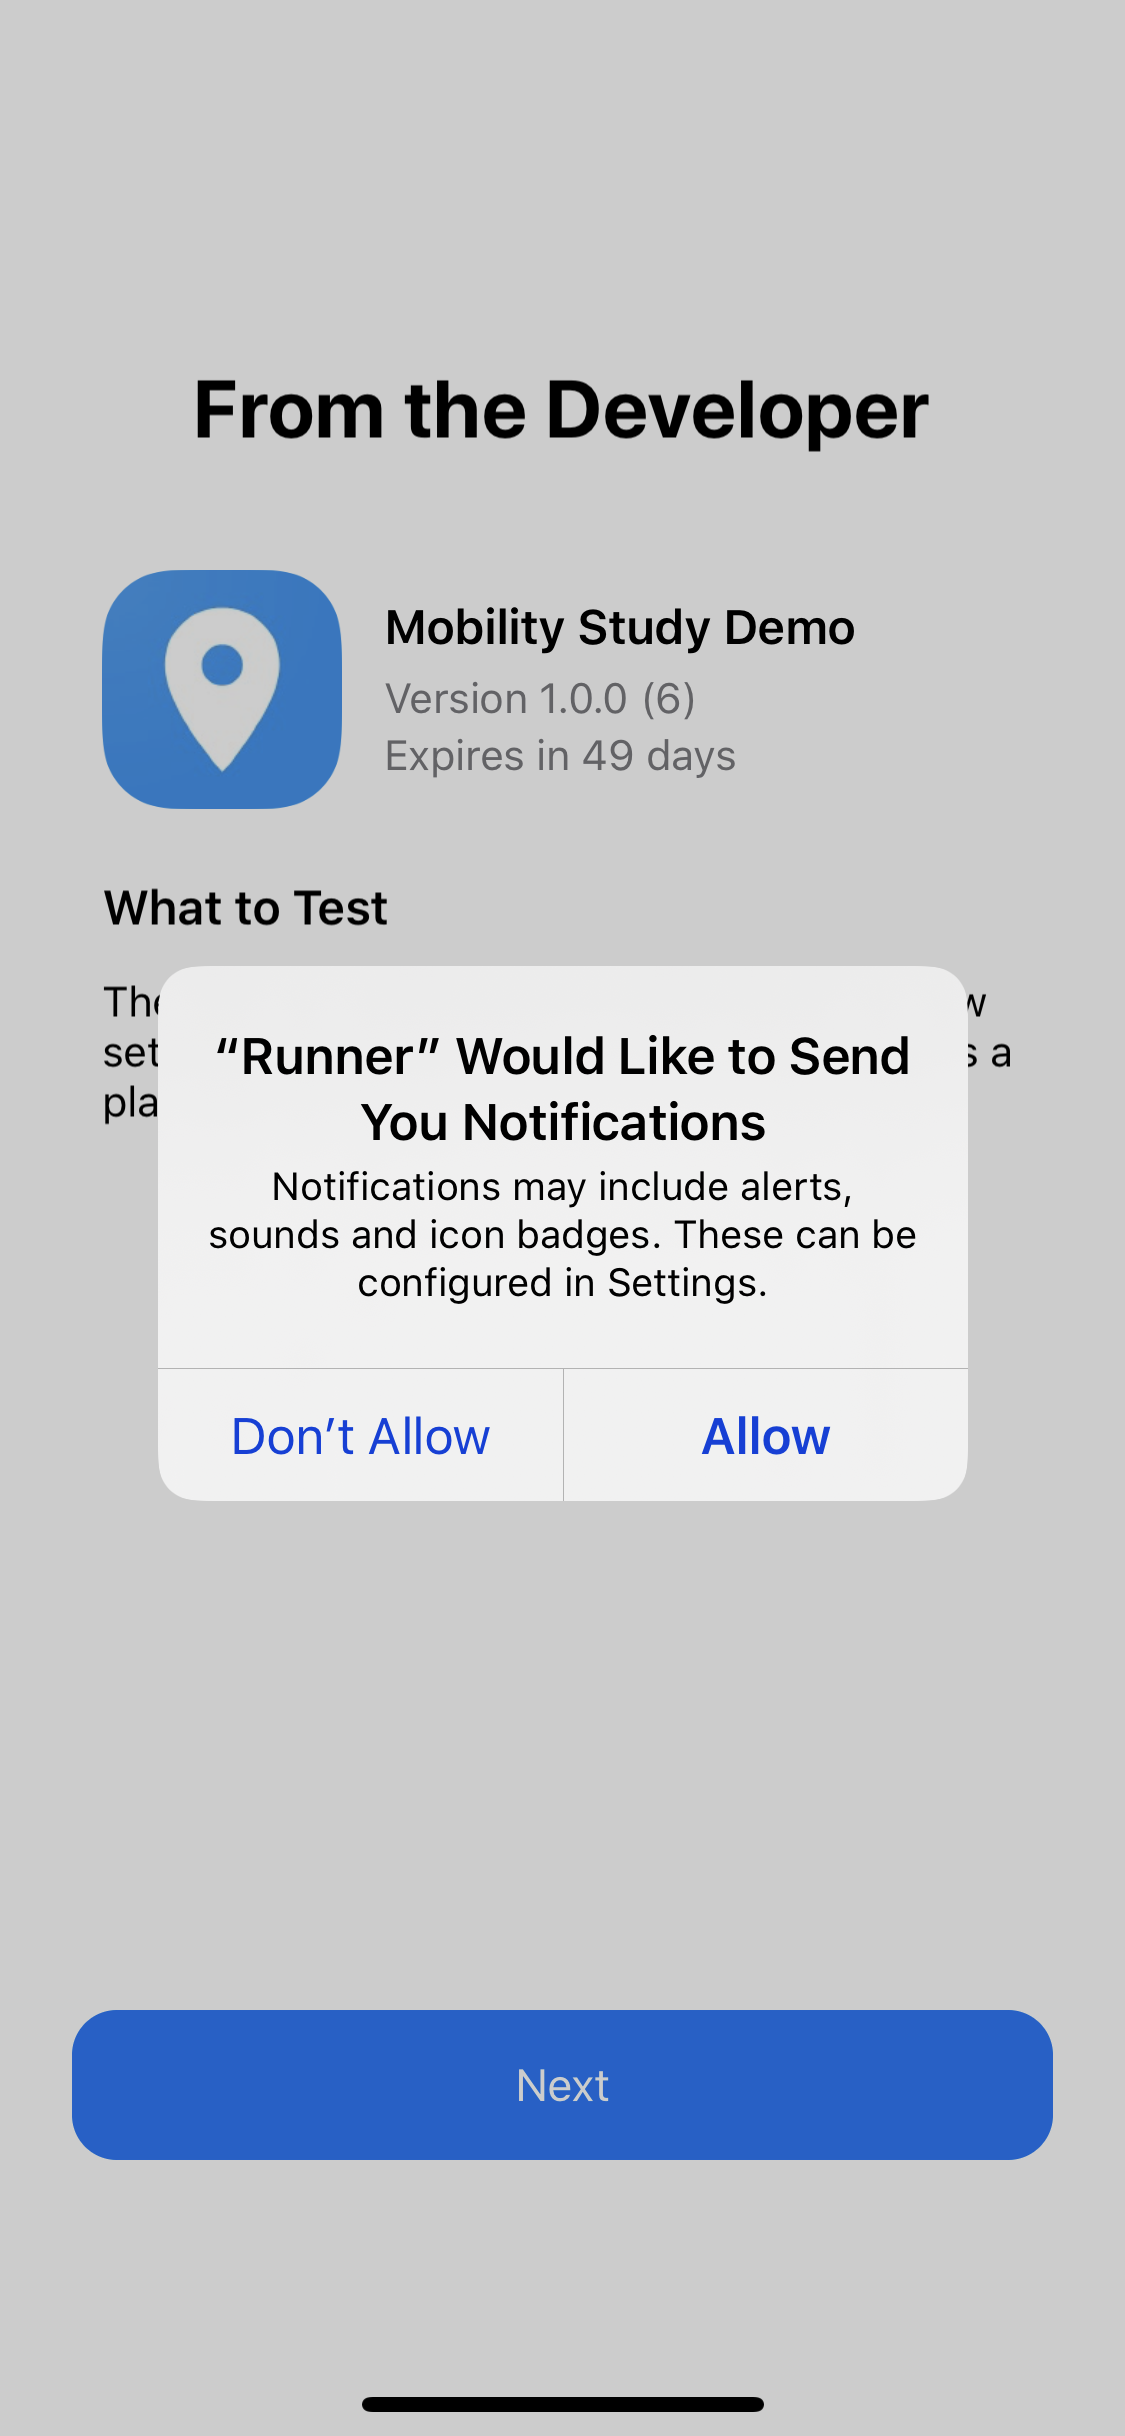
\includegraphics[width=0.2\textwidth]{images/app_imgs/app_permission.png} \includegraphics[width=0.2\textwidth]{images/app_imgs/app_notification.png}
    \caption{The initial installation- and setup process for the user}
    \label{fig:my_label}
\end{figure}

\subsection{App Screens}
The Main Page of the application merely displays a list of instructions to the user, but has two buttons in the navigation bar which can take the user to the Info Page and the Diary Page. The Info Page is made to inform the user of how the data will be used, and an email to contact the researcher in case of any questions.

\begin{figure}
    \centering
    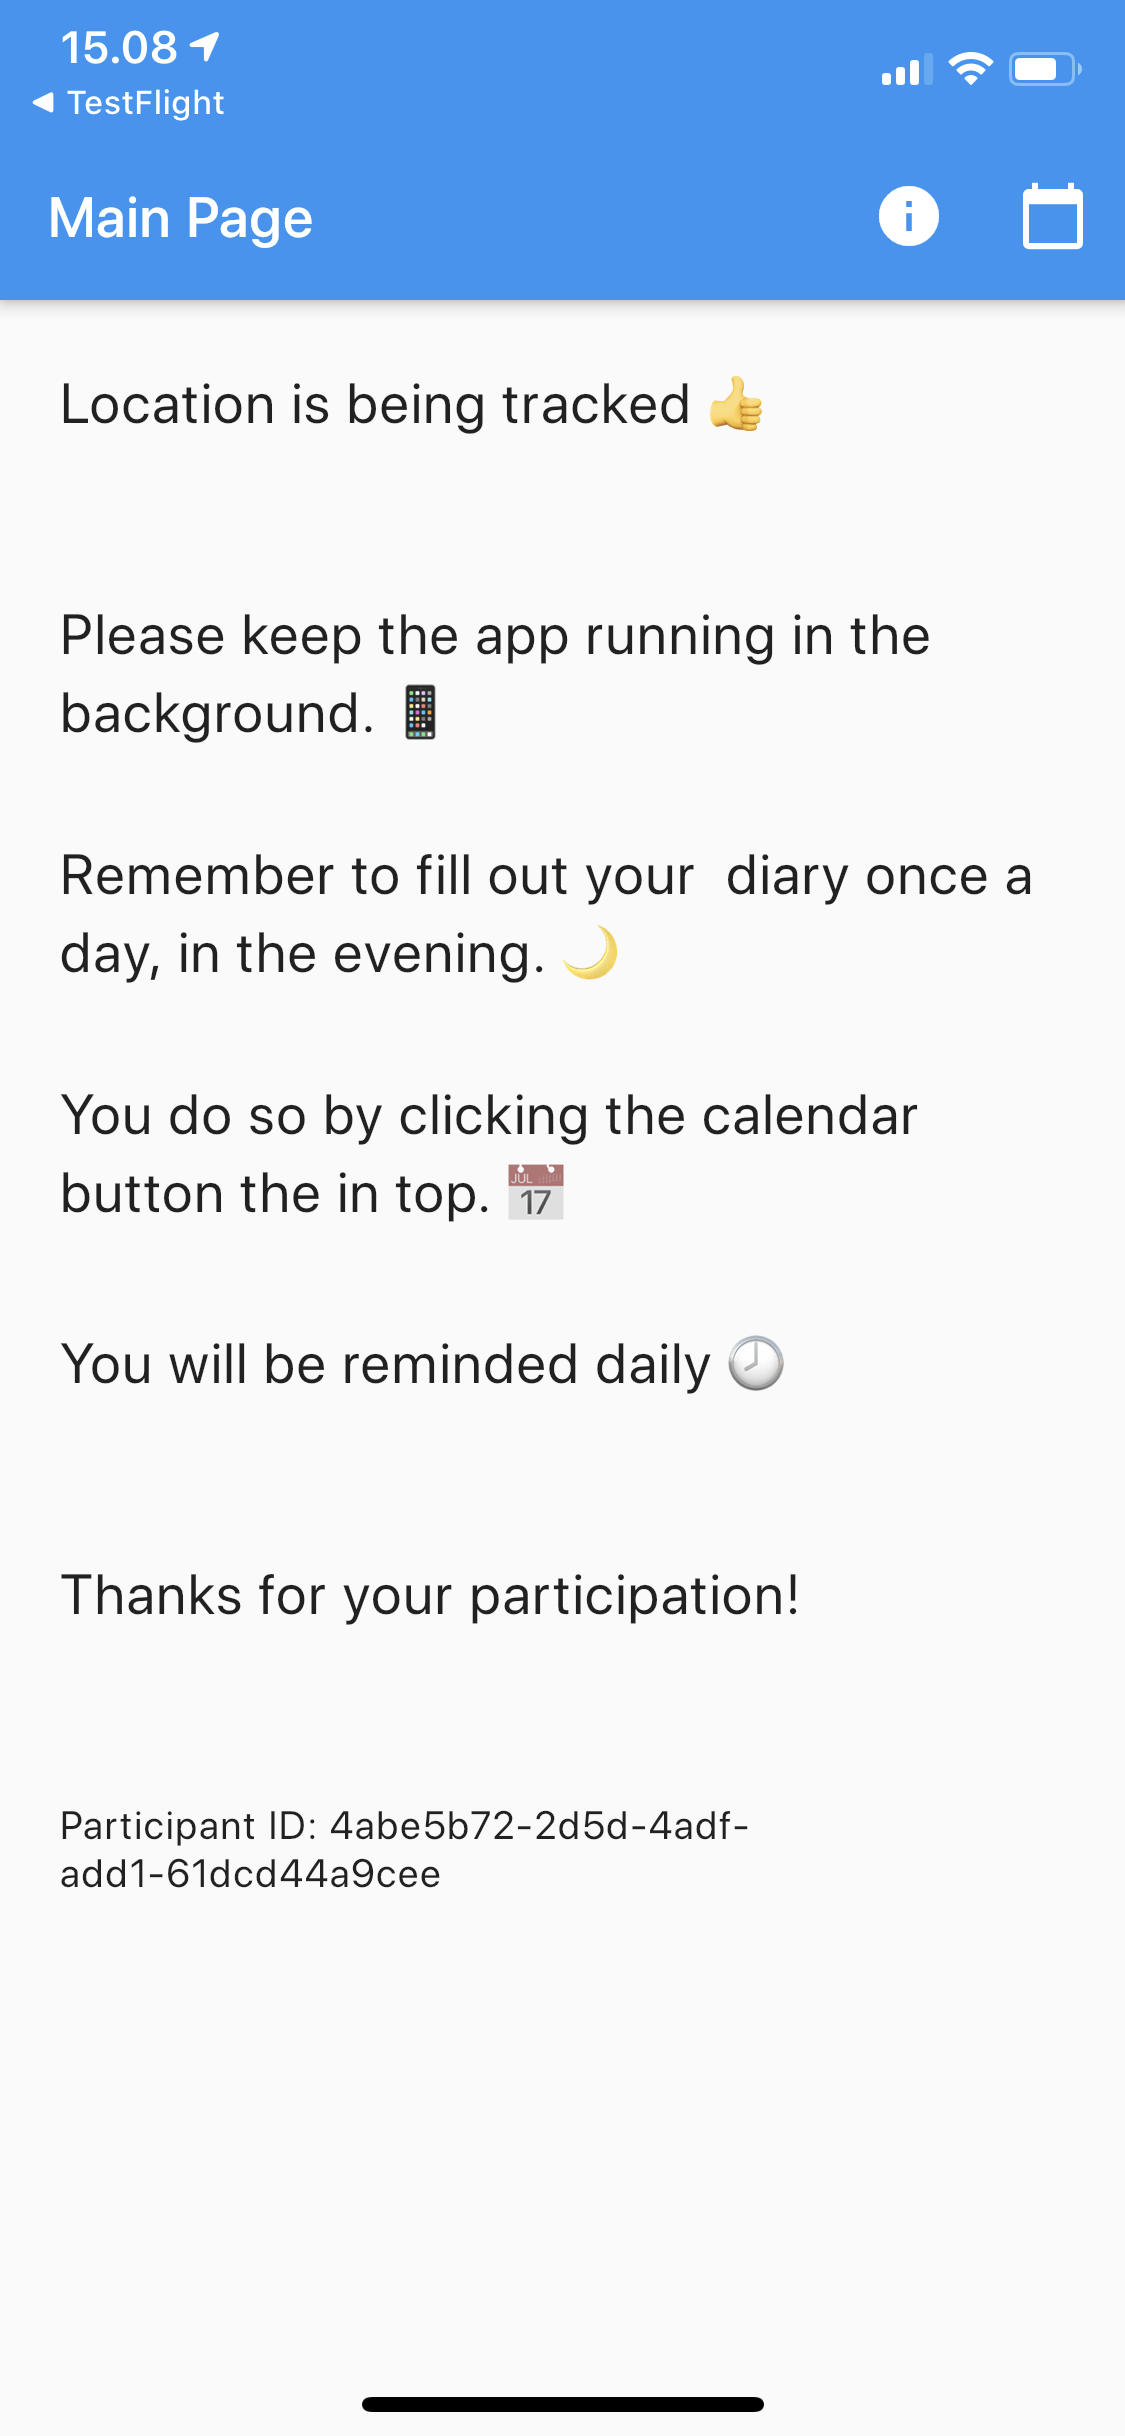
\includegraphics[width=0.2\textwidth]{images/app_imgs/app_mainpage.png} 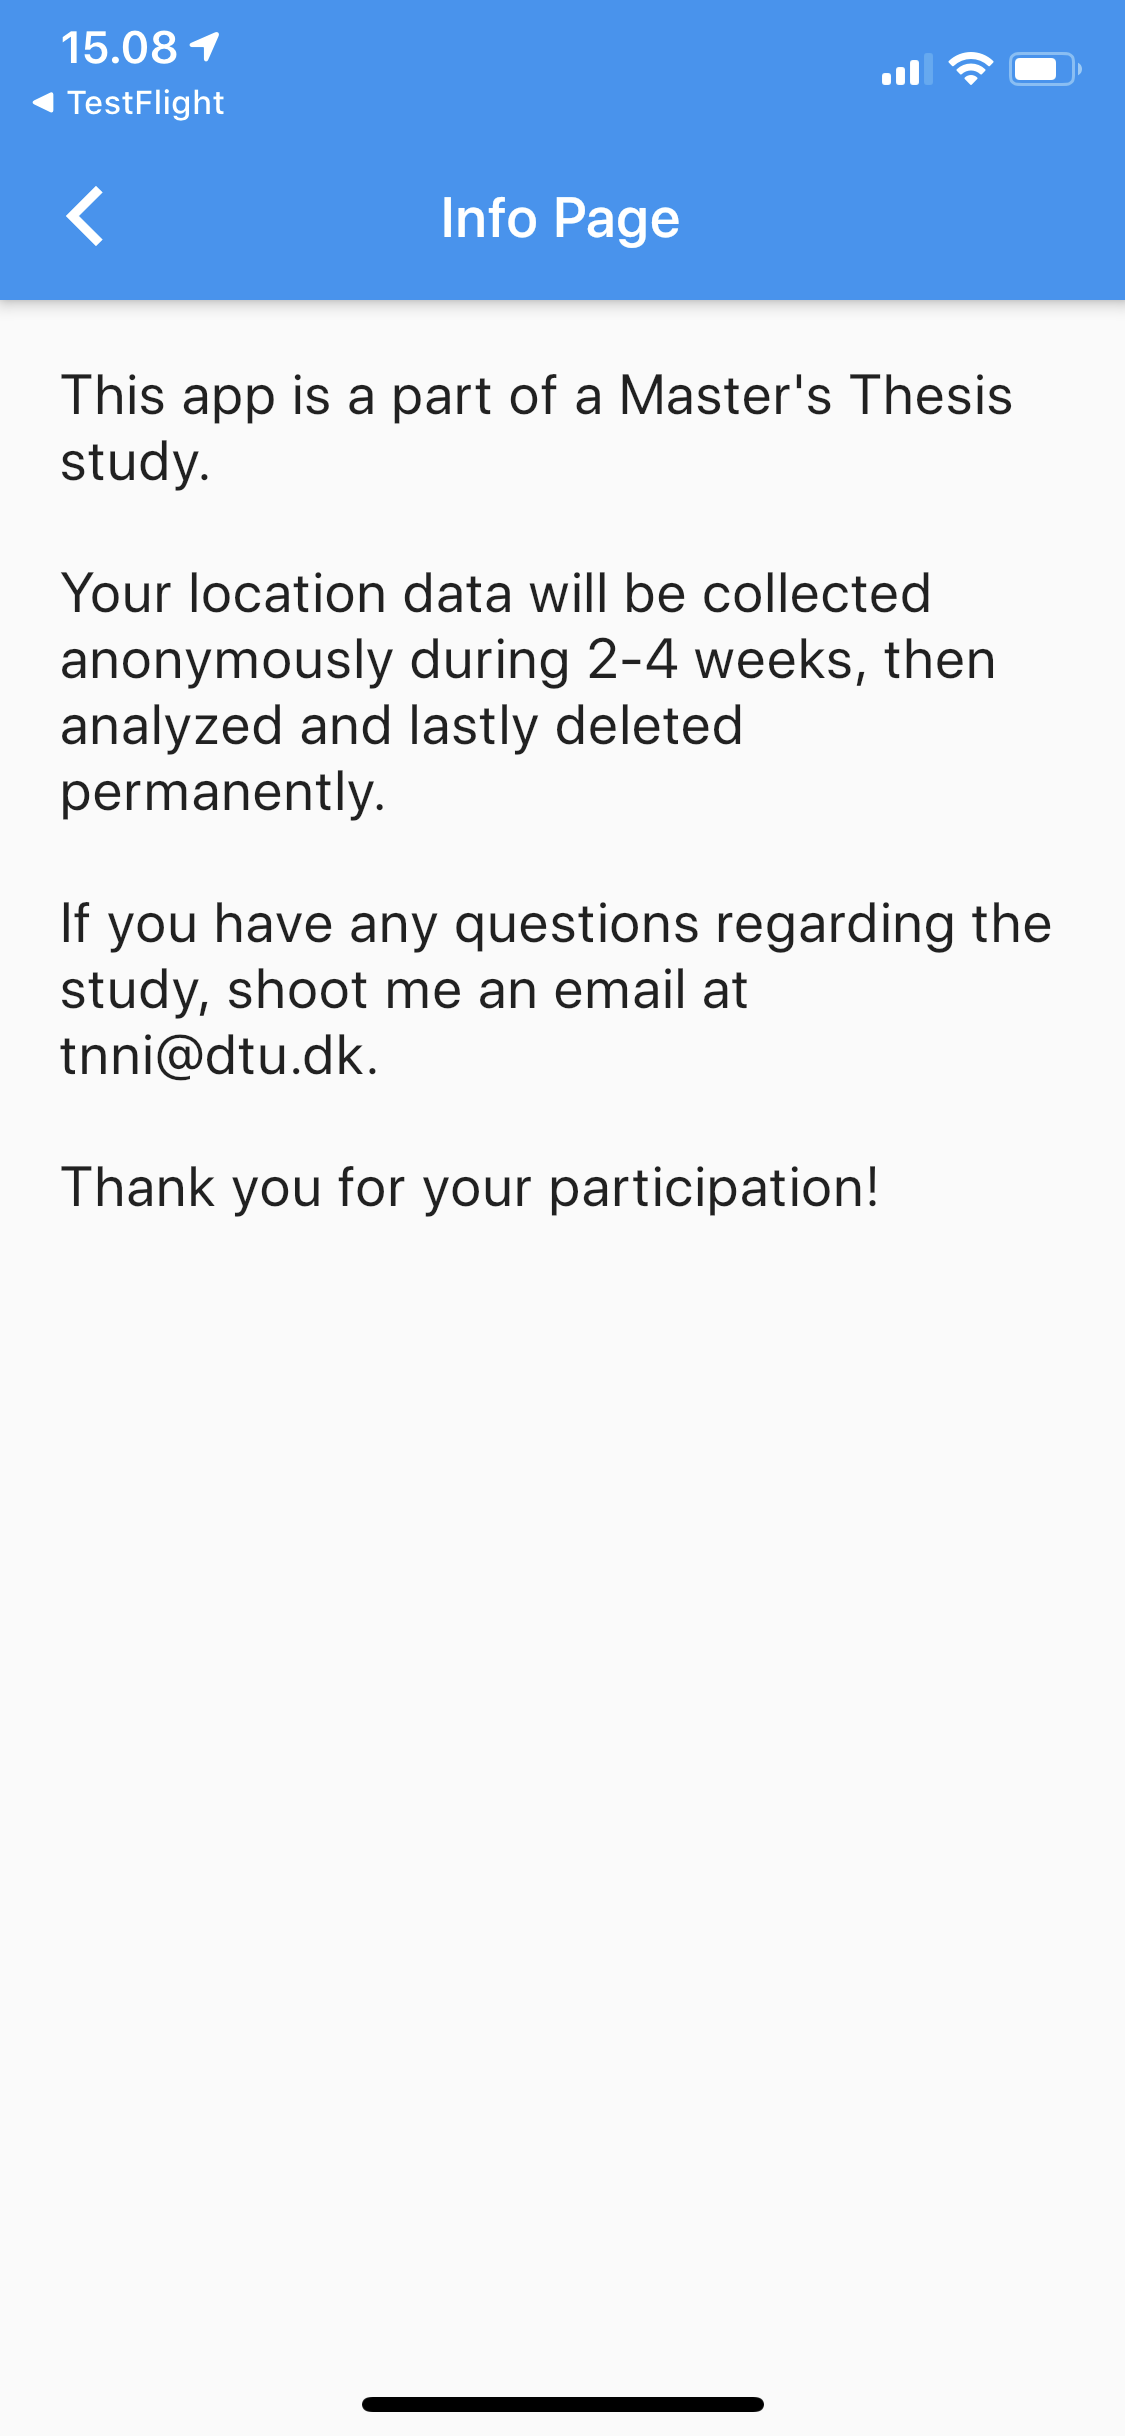
\includegraphics[width=0.2\textwidth]{images/app_imgs/app_infopage.png}
    \caption{The Main page and the Info Page which both contain little to no user interaction}
    \label{fig:my_label}
\end{figure}

The user navigates to the Diary Page by either tapping the calendar icon on the main page or by tapping the notification which comes in daily. In total there are four answers which answer answered by pressing the Answer button; this shows a wheel of possible values to pick from for providing an answer. Once all answers have been given, the submit button will be enabled and once pressed the answers will be stored on the device and sent to a server. When this is done, the last screen will appear which informs the user the answers have been saved and thanks them for their contribution.

\begin{figure}
    \centering
    \includegraphics[width=0.2\textwidth]{images/app_imgs/app_notification.png} 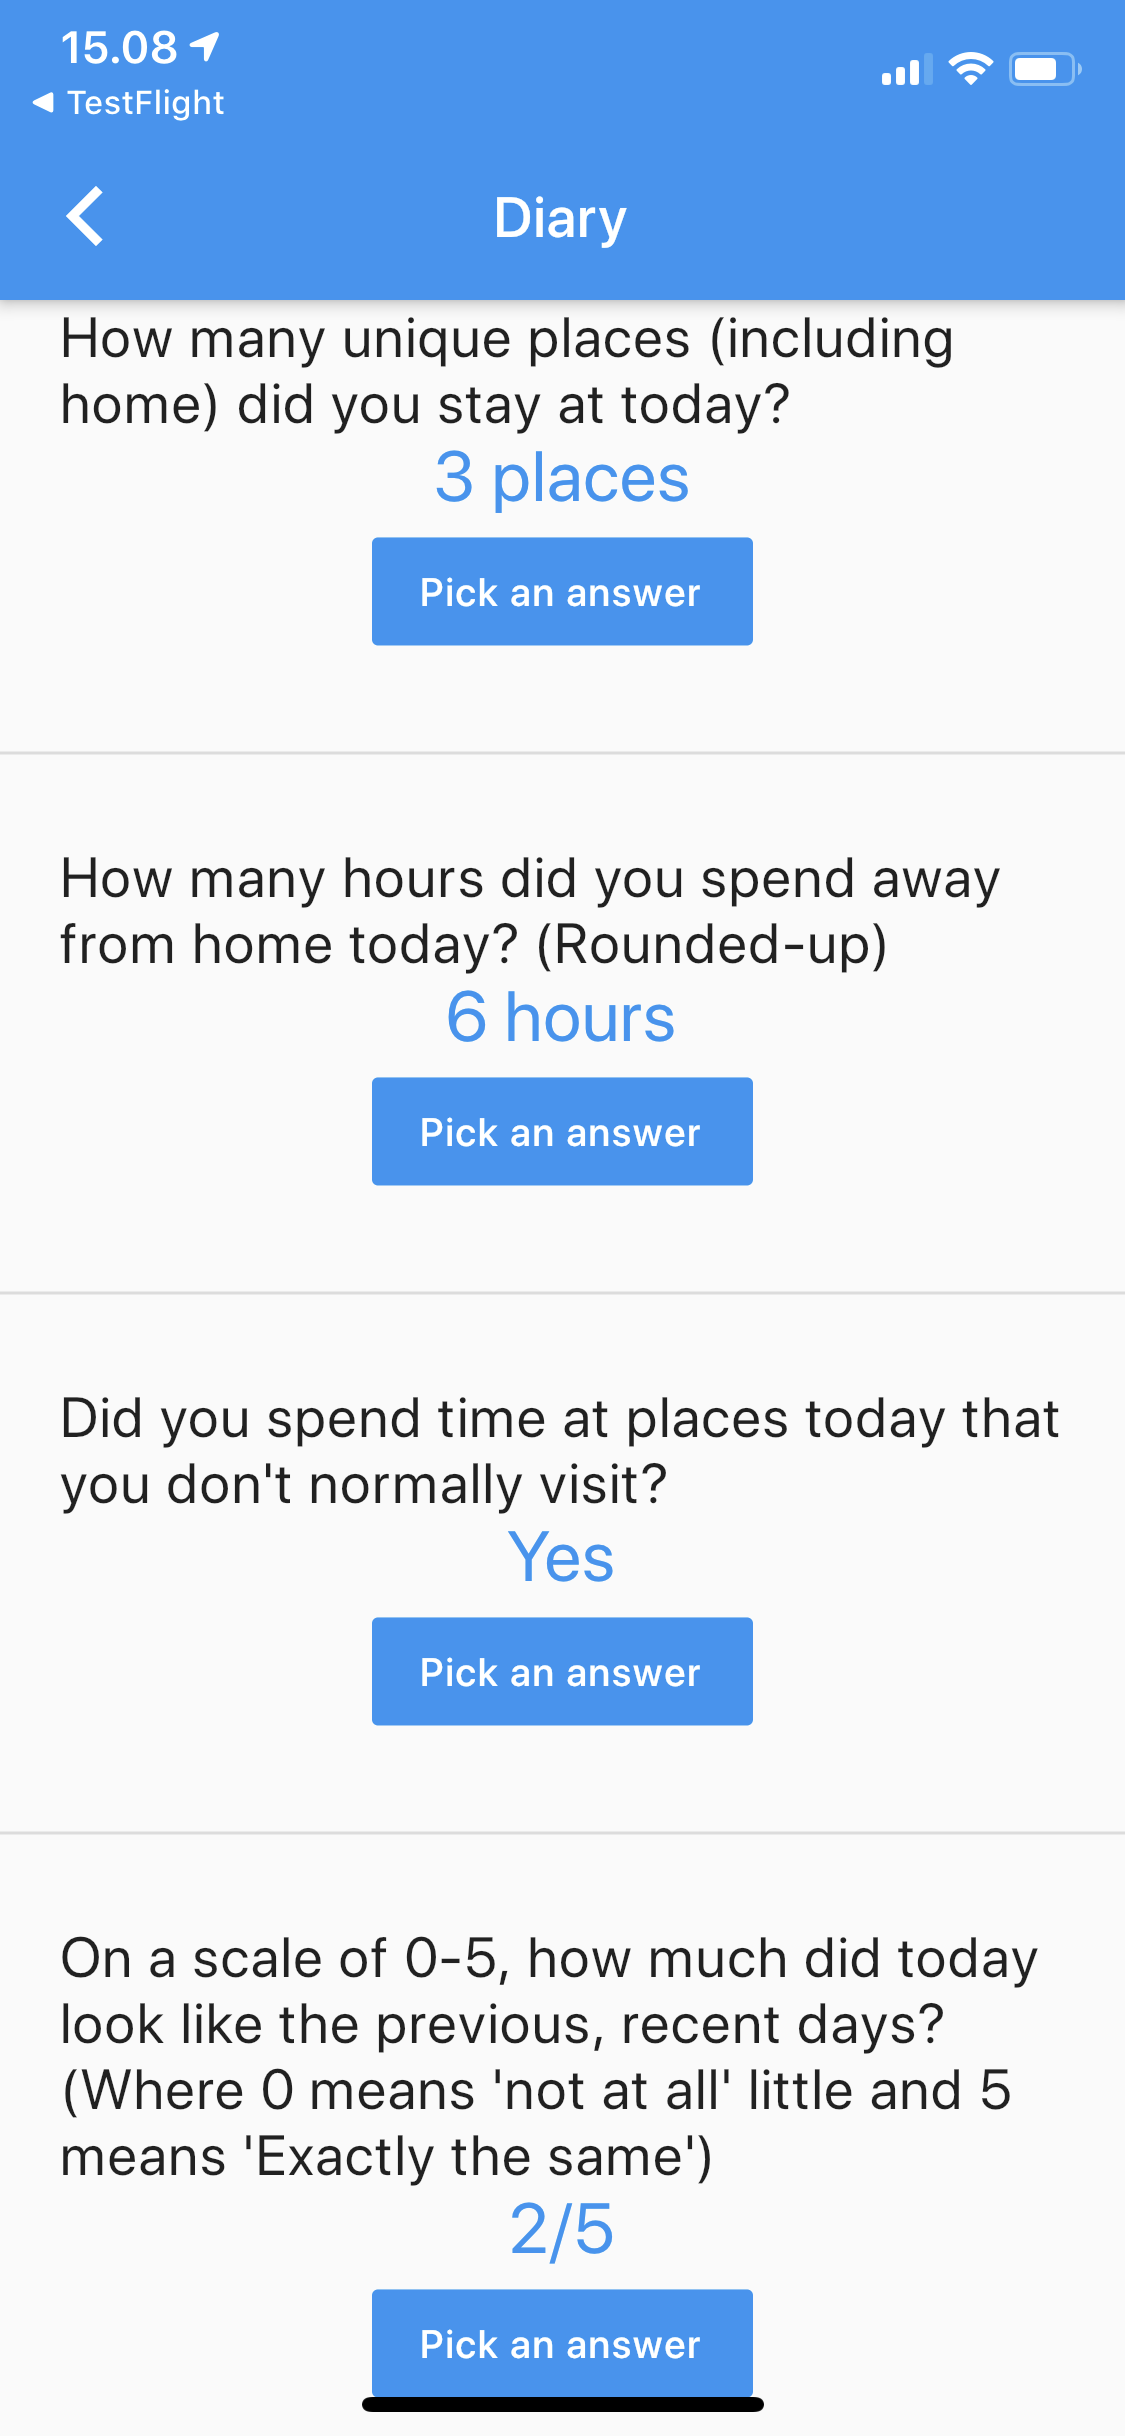
\includegraphics[width=0.2\textwidth]{images/app_imgs/app_noanswers.png}
    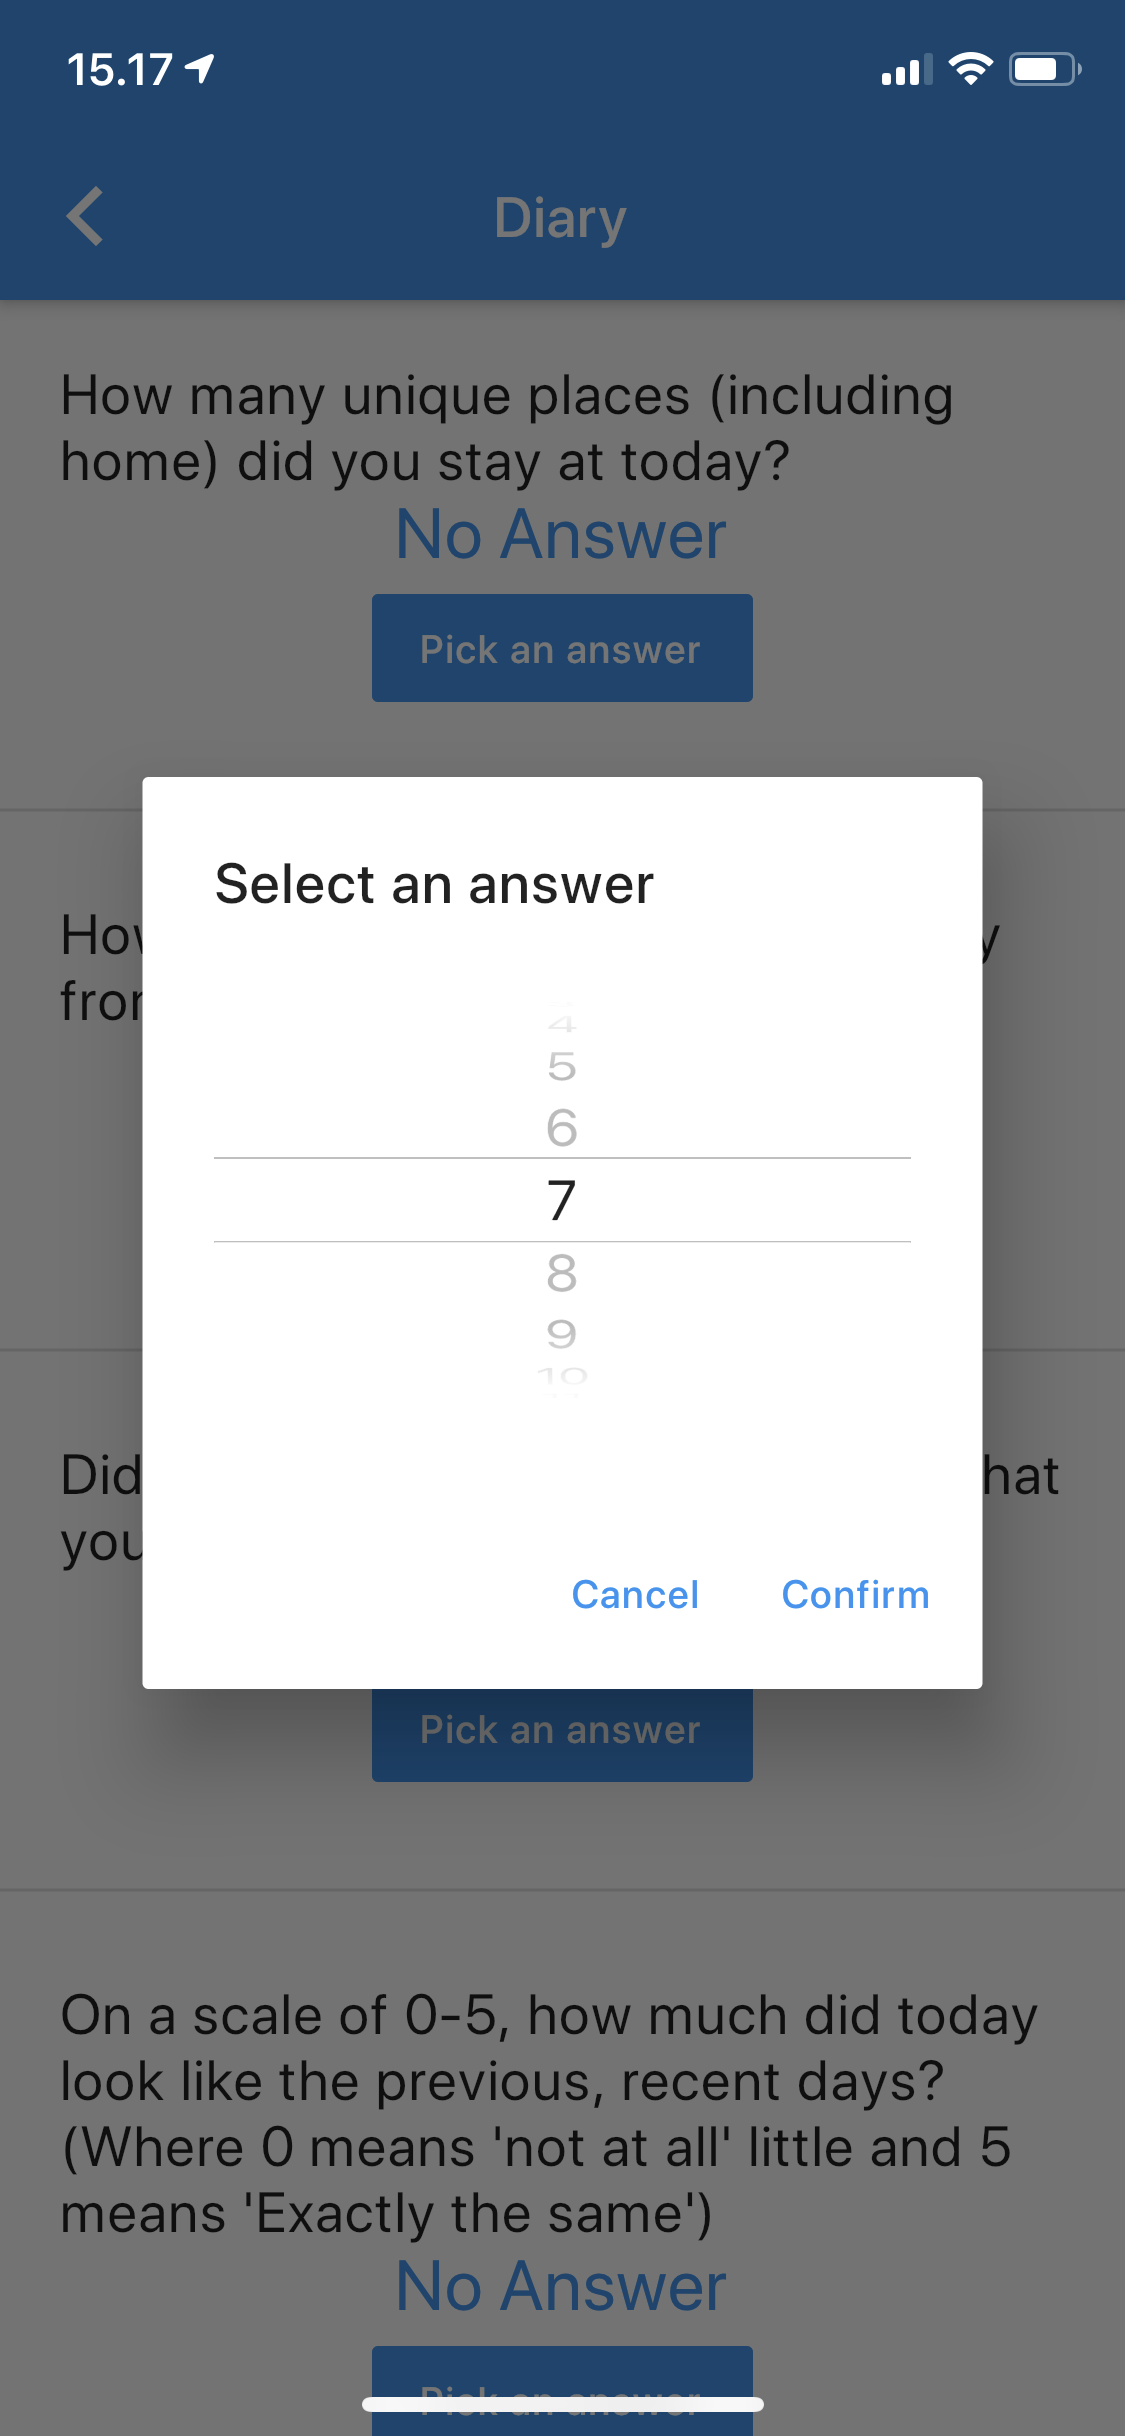
\includegraphics[width=0.2\textwidth]{images/app_imgs/app_answering.png} 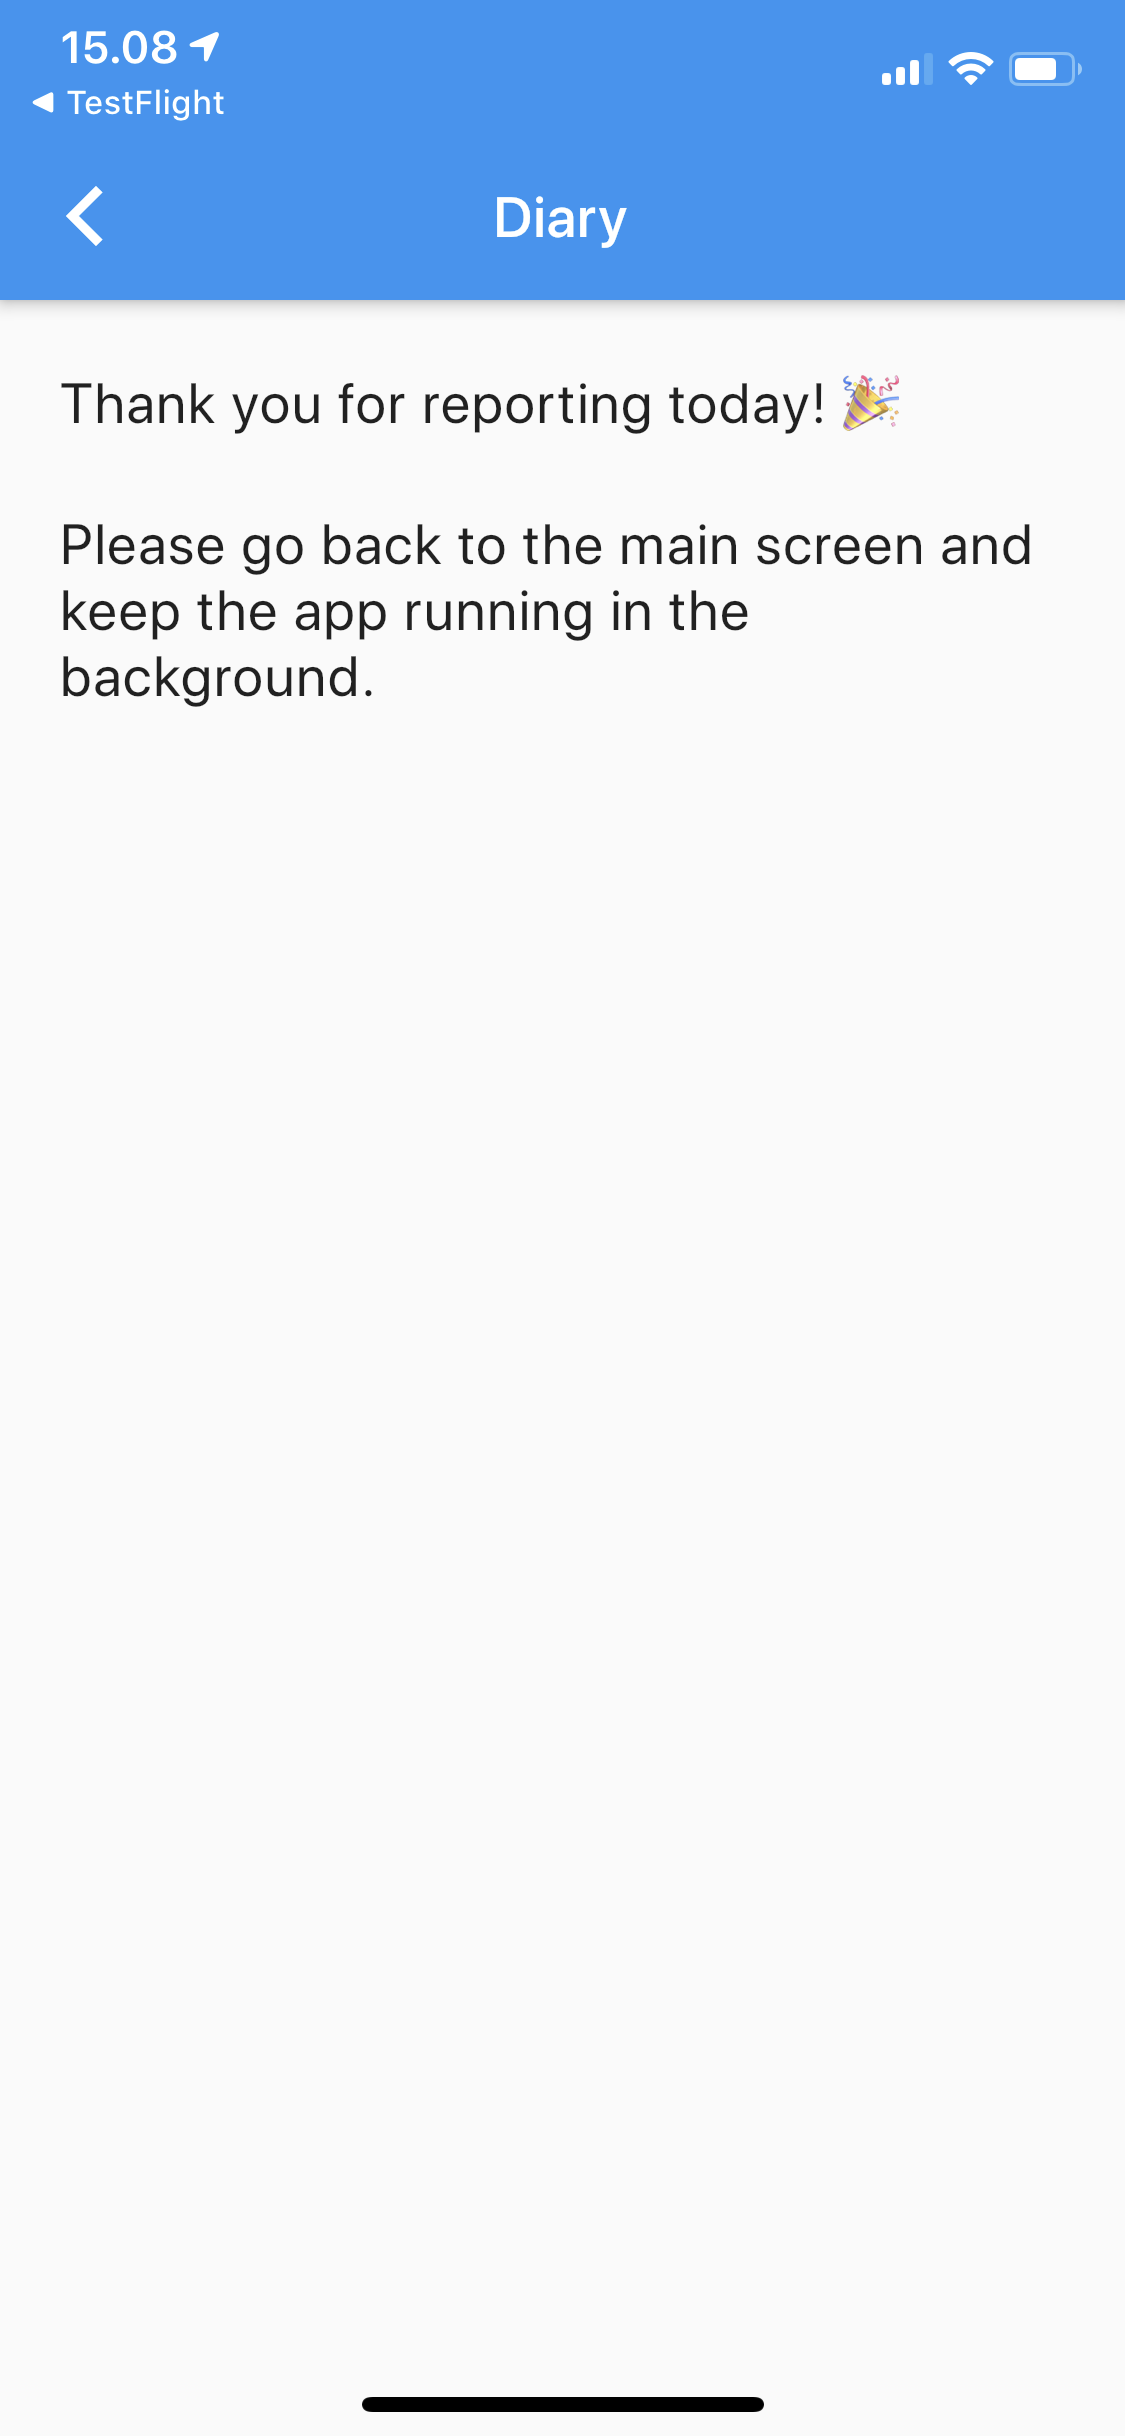
\includegraphics[width=0.2\textwidth]{images/app_imgs/app_submitted.png}
    \caption{The different screen states for the DiaryPage}
    \label{fig:my_label}
\end{figure}

\subsection{Displaying Features}
An initial version of the application included a display of the real-time calculated features, which were re-calculated each time a button was pressed. It was decided to not display the features in the final version for the study, since they would influence the answers given by the users. For example, if the application would state that the user has visited a certain number of places today, it is highly unlikely that a participant would report something else, if they are the least in doubt themselves. This display of features may be relevant (at least for some of the more features which are more easily interpret-able such as Home Stay) for a real-world application where it makes sense to inform the user exactly what goes on behind the curtain.

\section{Application Implementation}
This section will describe the implementation of the study application, mostly regarding how data was collected, how features were computed as well as how the data was sent to a Firebase instance. 

\subsection{Component Overview}
To provide a high level overview of the different components which make up the study application a component diagram displayed in Figure \ref{fig:app-component-diagram}. The MobilityStudy component in blue is the component responsible for managing the application state but does not do much outside of this since the application state management required is minimal. Had it been a more complex application with many different screens and a state which had to be maintained across these screens (for example a shopping cart in a shopping app) then more logic would lie inside the MobilityStudy component. Instead the Main Screen is spawned from the MobilityStudy component which in turn creates an AppProcessor instance. The AppProcessor instance is responsible for a multitude of tasks, such as asking for permissions, collection location data, and computing features. Storing and loading from the disk is done through the FileManager component which includes location data, Stops, Moves, MobilityContexts and diary answers. This component is also responsible for uploading the stored data to Firebase.

\begin{figure}
    \centering
    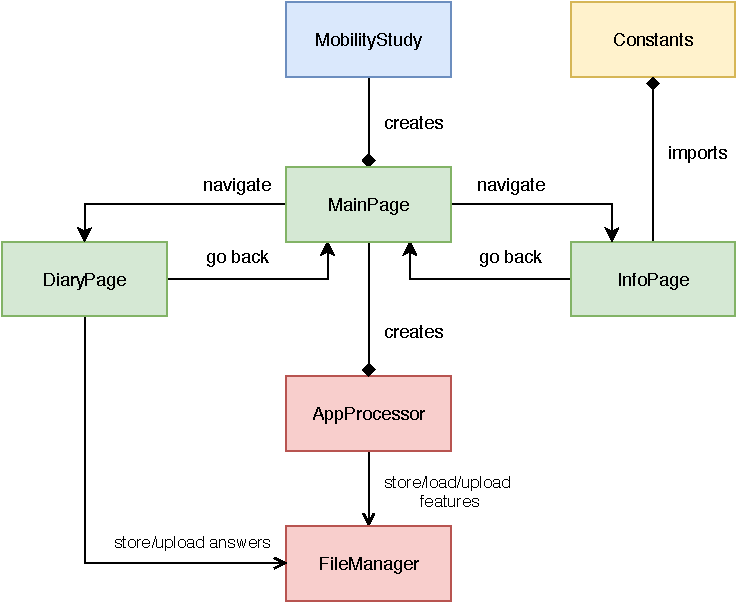
\includegraphics[width=\textwidth]{images/diagrams/app-diagram.pdf}
    \caption{Component diagram for the study application displaying the different building blocks and the interactions between them}
    \label{fig:app-component-diagram}
\end{figure}


\subsection{Location Collection}
The mobile application used the Mobility Features Package by importing it locally using an override as show in Figure \ref{fig:import-package}. As can be seen in the figure, the custom Geolocator plugin previously discussed was also imported in the same manner, since the online version on \url{www.pub.dev} does not allow for background location streaming. 

\begin{figure}
    \centering
    \begin{minted}{yaml}
    dependencies:
      geolocator:
        path: ../geolocator_custom/
      mobility_features:
        path: ../mobility_features/
    \end{minted}
    \caption{Importing the Mobility Features package as well as a custom Geolocator plugin in the \verb|pubspec.yaml| file}
    \label{fig:import-package}
\end{figure}

Next, the location tracking was set up using the Geolocator plugin, in which a stream subscription was initialized which in turn listens for new location data. Each time a new data point comes in, the call-back function \verb|_onData| is called, which handles the data collection. The function uses a buffer and a buffer size; whenever a new datapoint comes in, it is saved to the buffer and if the buffer capacity is reached then all points contained in the buffer are written to the disk, and the buffer is emptied. The lower the buffer size is, the more frequent the location data will be written to the disk.

\begin{figure}
    \centering
    \begin{minted}{dart}
    List<SingleLocationPoint> _pointsBuffer = [];
    static const int BUFFER_SIZE = 100;
    ...
    
    Future _initLocation() async {
        await _geoLocator.isLocationServiceEnabled().then((response) {
          if (response) {
            streamingLocation = true;
            _subscription = _geoLocator.getPositionStream().listen(_onData);
          } else {
            print('Location service not enabled');
          }
        });
    }
    ...
    
    void _onData(Position d) async {
        SingleLocationPoint p =
            SingleLocationPoint(Location(d.latitude, d.longitude), d.timestamp);
        _pointsBuffer.add(p);
    
        // Check if buffer should be saved to disk
        if (_pointsBuffer.length >= BUFFER_SIZE) {
          ...
        }
    }
    \end{minted}
    \caption{Importing the Mobility Features package as well as a custom Geolocator plugin in the \verb|pubspec.yaml| file}
    \label{fig:import-package}
\end{figure}



\subsection{Storing, Loading and Uploading}
Storing and loading SLPs, Stops and Moves work through the serialization API provided by the Mobility Features Package discussed in Chapter \ref{chapter:05}. Concretely a \verb|Serializer<E>| object is created for each type in the AppProcessor class, and are used to store and load their given type \verb|E|. Below is shown an example of this:



\begin{figure}
    \centering
    \begin{minted}{dart}
    Serializer<SingleLocationPoint> _pointSerializer;
    
    ...
    Future<List<SingleLocationPoint>> _loadLocalPoints() async {
        DateTime today = DateTime.now().midnight;
        print('Loading local data points...');
        List<SingleLocationPoint> points = await _pointSerializer.load();
        if (points.isEmpty) {
          return points;
        } else if (points.first.datetime.midnight.isBefore(today)) {
          print('Old location data found, deleting it...');
          points = points.where((p) => p.datetime.midnight == today).toList();
          await _pointSerializer.flush();
          await _pointSerializer.save(points);
        }
        return points;
    }
    \end{minted}
    \caption{The procedure for loading the locally saved SLPs, including filtering out SLPs from previous days}
    \label{fig:points-serialization}
\end{figure}


Whenever new data comes in, the \verb|_onData| callback-method is invoked as previously mention, which collects the new data point in a buffer, which when full is stored to the disk. This is also done by using the Serializer:

\begin{minted}{dart}
if (_pointsBuffer.length >= BUFFER_SIZE) {
    await _pointSerializer.save(_pointsBuffer);
    _pointsBuffer = [];
}
\end{minted}


Saving and loading Stops and Moves is done in a very similar fashion, namely by using separate Serializers. In the case that a MobilityContext is to be computed, the Stops and Moves on disk are loaded with the following source code:

\begin{minted}{dart}
    List<Stop> stops = await _stopSerializer.load();
    List<Move> moves = await _moveSerializer.load();
\end{minted}

After computation, the new-found Stops and Moves are to replace the old ones, which means the Serializers should flush their files, and then store the new data. Given a MobilityContext object \verb|MobilityContext mc| which contains the new Stops and Moves, the parameterless method \verb|flush| is first called, and afterwards the \verb|save| method is called with the new data to be stored.
\begin{minted}{dart}
    await _stopSerializer.flush();
    await _moveSerializer.flush();

    await _stopSerializer.save(mc.stops);
    await _moveSerializer.save(mc.moves);
\end{minted}

\subsection{Computing Features}
Feature calculation was done in an asynchronous manner, in which the work was offloaded to a background thread, rather than running on the main thread. The reason for this is that if the calculation is done on the main thread, then the app will be un-responsive while the computation is being carried out. In the study app there was no real user interface so to speak, but in a real-world application there will be a user interface which cannot be allowed to freeze due to the feature calculation. In FLutter threads are referred to as Isolates which communicate using a SendPort and a ReceivePort. These ports can be used to transfer objects between threads, such that the main thread can ask a background thread to calculate the features, and the background thread will then send back a \textit{MobilityContext} object once finished. To calculate the features, the intermediate features Stops, Moves and Places were calculated first. All this is described by the sequence diagram in Figure \ref{fig:sequence-diagram-mobility-context}, in Chapter \ref{chapter:05}. In figure \ref{fig:feature-comutation-code} source code for achieving this in the flutter app is shown. The \verb|_relay| method works an interface between the \verb|_computeFeaturesAsync| method which runs on the UI thread and the static method \verb|_asyncComputation| which runs on the background thread.


\begin{figure}
    \centering
    \begin{minted}{dart}
    Future<MobilityContext> _computeFeaturesAsync() async {
        // Load from disk
        List<Stop> stops = await _stopSerializer.load();
        List<Move> moves = await _moveSerializer.load();
        List<SingleLocationPoint> points = await _loadLocalPoints();
        
        // Set up background thread
        ReceivePort receivePort = ReceivePort();
        await Isolate.spawn(_asyncComputation, receivePort.sendPort);
        SendPort sendPort = await receivePort.first;
        
        // Off-load computation to background thread, and await
        return await _relay(sendPort, points, stops, moves);
    }
    
    Future _relay(SendPort sp, List<SingleLocationPoint> points, 
                    List<Stop> stops, List<Move> moves) {
    ReceivePort receivePort = ReceivePort();
    sp.send([points, stops, moves, receivePort.sendPort]);
    return receivePort.first;
  }
    \end{minted}
    \caption{The method for querying the Mobility Feature computation on the UI thread}
    \label{fig:feature-comutation-code}
\end{figure}


The \verb|_asyncComputation| method is static which is due to the computation being done in a separate thread than than the main thread. If the objects contained within the AppProcessor instance (i.e. in the main thread) were to change their state while computation was ongoing in the background thread, then the resulting computation would produce an outdated, and or wrong result. To circumvent this, the method that performs the computation relies on parameters instead, i.e. the SLPs, Stops and Moves must be explicitly provided. Concretely, a copy of the objects are created when fed to the static method as parameters. These copies can then have their state modified only inside the static method and not outside which results in the computation being reliable wrt. state management. 

The computation will be discussed bit for bit such a to give the reader a better overview of the implementation:

Firstly the arguments are parsed from the sendport; the arguments come in as an array and are therefore simply extracted via indices.
\begin{minted}{dart}
  static void _asyncComputation(SendPort sendPort) async {
    ReceivePort receivePort = ReceivePort();
    sendPort.send(receivePort.sendPort);
    List args = await receivePort.first;

    /// Extract arguments
    List<SingleLocationPoint> points = args[0];
    List<Stop> stops = args[1];
    List<Move> moves = args[2];
    SendPort replyPort = args[3];
    ...
  }
\end{minted}

Secondly, the date 28 days from today is calculated and from this date a filtering process for the loaded Stops and Moves is performed. This process removes all the loaded Stops and Moves which are today, or older than four weeks from today. The reason for removing data from today is that it must be recalculated using all the data points from today, in order to be precise. Secondly data older than 28 days is discarded since it is no longer relevant, the concrete reasons are discussed in Chapter \ref{chapter:03}.
\begin{minted}{dart}
    DateTime today = DateTime.now().midnight;
    DataPreprocessor preprocessor = DataPreprocessor(today);
    DateTime fourWeeksAgo = today.subtract(Duration(days: 28));

    /// Filter out stored stops and moves which were computed today,
    /// as well as stops older than 4 weeks
    List<Stop> stopsOld = stops.isEmpty
        ? stops
        : stops
            .where((s) =>
                s.arrival.midnight != today.midnight &&
                fourWeeksAgo.leq(s.arrival.midnight))
            .toList();

    List<Move> movesOld = moves.isEmpty
        ? moves
        : moves
            .where((m) =>
                m.stopFrom.arrival.midnight != today.midnight &&
                fourWeeksAgo.leq(m.stopFrom.arrival.midnight))
            .toList();
\end{minted}

Thirdly, today's data points are used to find the most updated set of Stops and Moves for today, which are then concatenated with the old stops and moves. From this set of intermediate features covering the last 28 days the corresponding Places for the period can now be found.

\begin{minted}{dart}
    /// Calculate stops and moves from today
    List<Stop> stopsToday = preprocessor.findStops(points, filter: false);
    List<Move> movesToday = preprocessor.findMoves(points, stopsToday, filter: false);

    /// Concatenate old and new, and compute places
    List<Stop> stopsAll = stopsOld + stopsToday;
    List<Move> movesAll = movesOld + movesToday;
    List<Place> placesAll = preprocessor.findPlaces(stopsAll);
\end{minted}

Lastly, the MobilityContex is computed from the intermediate features from the whole period
\begin{minted}{dart}
    /// Compute features
    MobilityContext mobilityContext = MobilityContext(today, stopsAll, placesAll, movesAll);
    replyPort.send(mobilityContext);
\end{minted}   

\chapter{Discussion}
\label{chapter:07}
\section{Data Analysis of Study}
As discussed, the participants had to fill out a small questionnaire every day in the evening and these answers were then matched against the computed results. The study resulted in a dataset with 205 days of data, corresponding to 2.51M timestamped location data points, spread over 10 participants. Table \ref{tab:location-samples} shows the overview of the data collected for each participant, including the number of points, number of days and the storage requirements for the collected data.\\

Similar to Cuttone et al. \cite{sparse-location-2014}, the participants have been anonymized as \textit{P1} through \textit{P9}, and the author has been marked as \textit{R} (researcher).\\

\begin{table}[]
    \centering
        \begin{tabular}{|l|l|l|l|l|l|}
        \hline
        {\ul \textbf{P}} & {\ul \textbf{Days}} & {\ul \textbf{Samples}} & {\ul \textbf{MB}} & {\ul \textbf{Samples/day}} & {\ul \textbf{MB/day}} \\ \hline
        \textbf{P1}                & 23                   & 181                        & 17.3                           & 7878.8                              & 0.8                              \\ \hline
        \textbf{P2}                & 25                   & 142                        & 13.6                           & 5684.4                              & 0.5                             \\ \hline
        \textbf{P3}                & 21                   & 101                        & 9.7                            & 4850.7                              & 0.5                             \\ \hline
        \textbf{P4}                & 22                   & 98                         & 9.4                            & 4494.9                              & 0.4                             \\ \hline
        \textbf{P5}                & 14                   & 209                        & 20.0                           & 14977.4                             & 1.4                             \\ \hline
        \textbf{P6}                & 26                   & 101                        & 9.7                            & 3922.8                              & 0.4                             \\ \hline
        \textbf{P7}                & 23                   & 111                       & 106.4                          & 48525.0                             & 4.6                             \\ \hline
        \textbf{P8}                & 15                   & 141                        & 13.5                           & 9417.3                              & 0.9                              \\ \hline
        \textbf{P9}                & 12                   & 51                         & 4.9                            & 4311.7                              & 0.4                              \\ \hline
        \textbf{R}                 & 24                   & 365                        & 34.9                           & 15233.6                             & 1.5                                    \\ \hline
        \end{tabular}

    \caption{The overview of collected Location Samples for each participant in the study}
    \label{tab:location-samples}
\end{table}

The answers were of a different format than the computed features and therefore had to be converted into scalars such that they could be compared directly to the features. For the Home Stay feature, the answer the users gave was the number of hours away from home, at the time of registering. It was assumed that most people be registering at home since the diary was filled out in the evening. Therefore for calculating the Home Stay value from a given answer $a$, equation \ref{eq:home-stay-ans} was applied:

\begin{equation}
\label{eq:home-stay-ans}
    h = \frac{t - a }{t}
\end{equation}

Here, $t$ refers to the timestamp at which the diary was filled out.

For the \textit{Routine Index}, the answer (a number of 0 to 5) was transformed to scalar between 0 and 1, i.e. let the scale value be $s \in \{0, 1, 2, 3, 4, 5\}$, then the corresponding \textit{Routine Index} is calculated using equation \ref{eq:routine-ans}.

\begin{equation}
\label{eq:routine-ans}
    r = \frac{s}{s_{max}}, \quad s_{max} = 5
\end{equation}

Regarding data collection, figure \ref{fig:plot-num-points-stops} displays how much data was collected per participant. From this figure, it is clear that some participants did not collect nearly as much data as others, and because of this their computed features are expected to be more inaccurate. It was also discovered that the number of stops found is not necessarily correlated with the number of location samples found, as can be seen for participant P7. This can be due to reasons such as moving around much less, which results in fewer but stops with a longer duration being found. \\

\begin{figure}
    \centering
    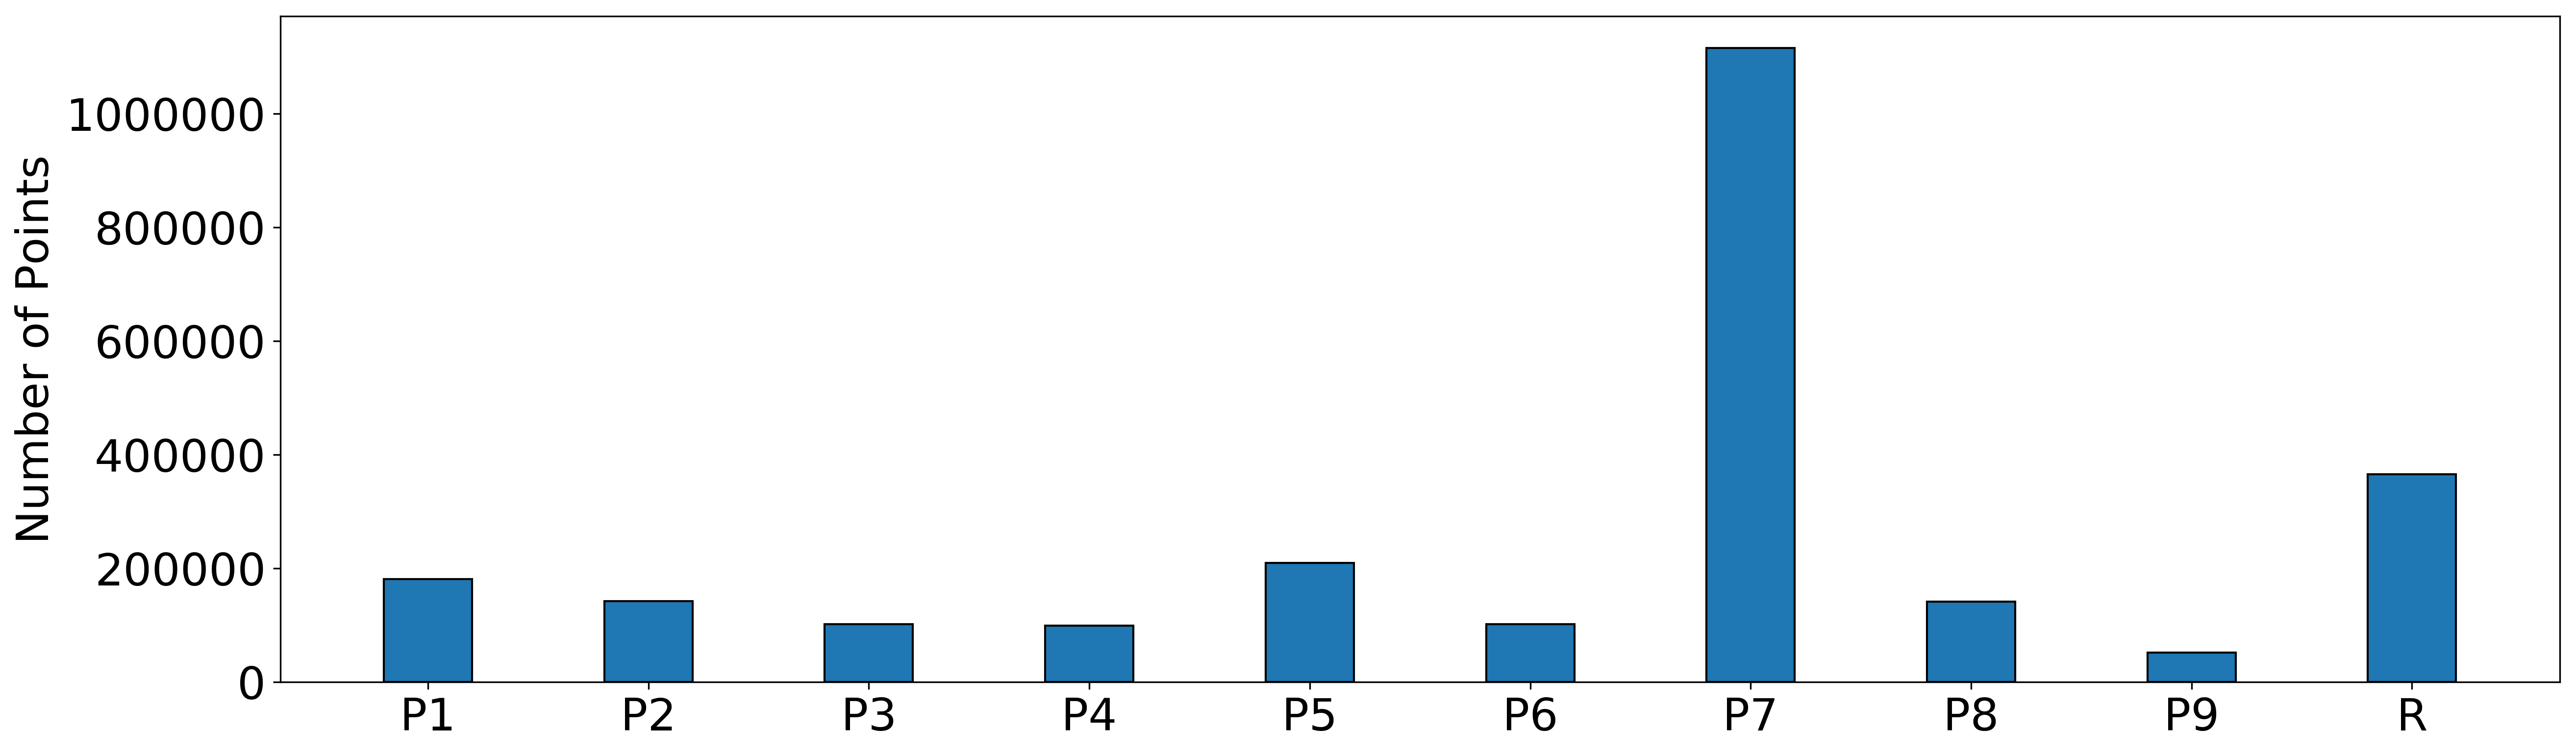
\includegraphics[width=\textwidth]{images/study/storage/num_points.png}
    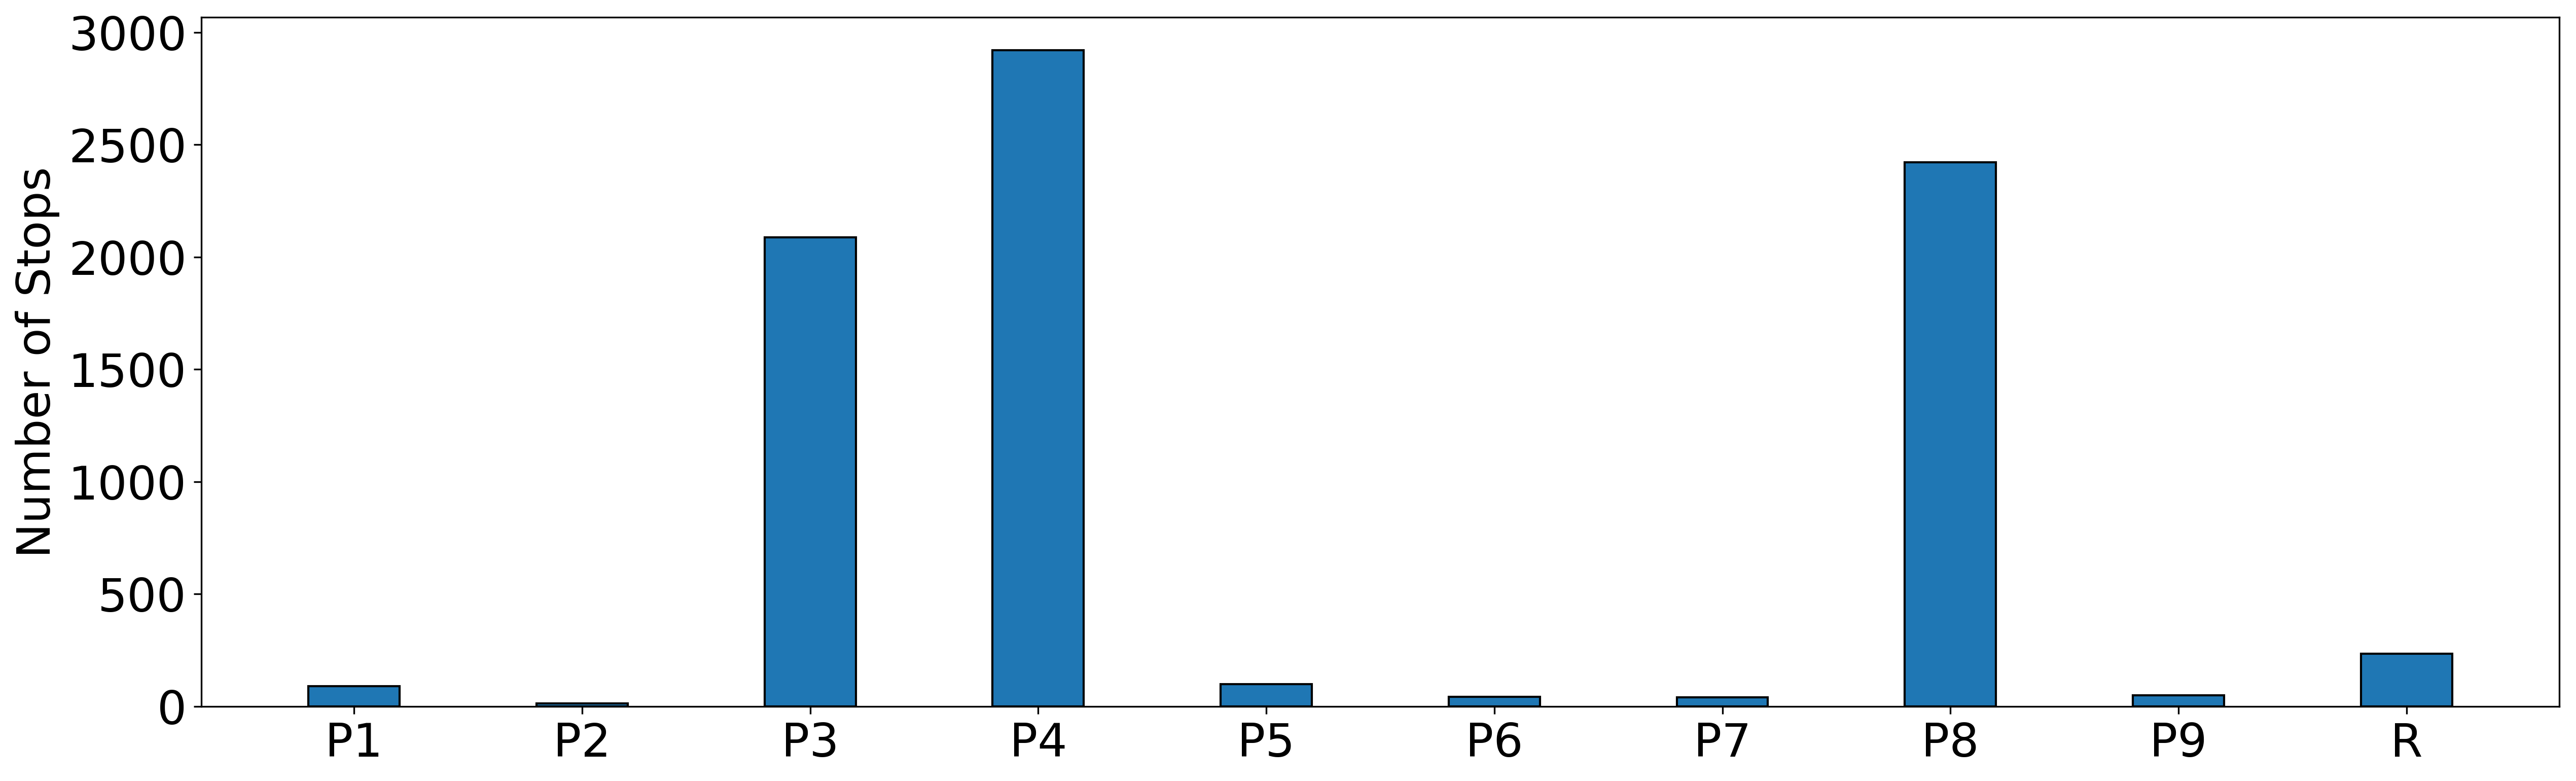
\includegraphics[width=\textwidth]{images/study/storage/num_stops.png}
    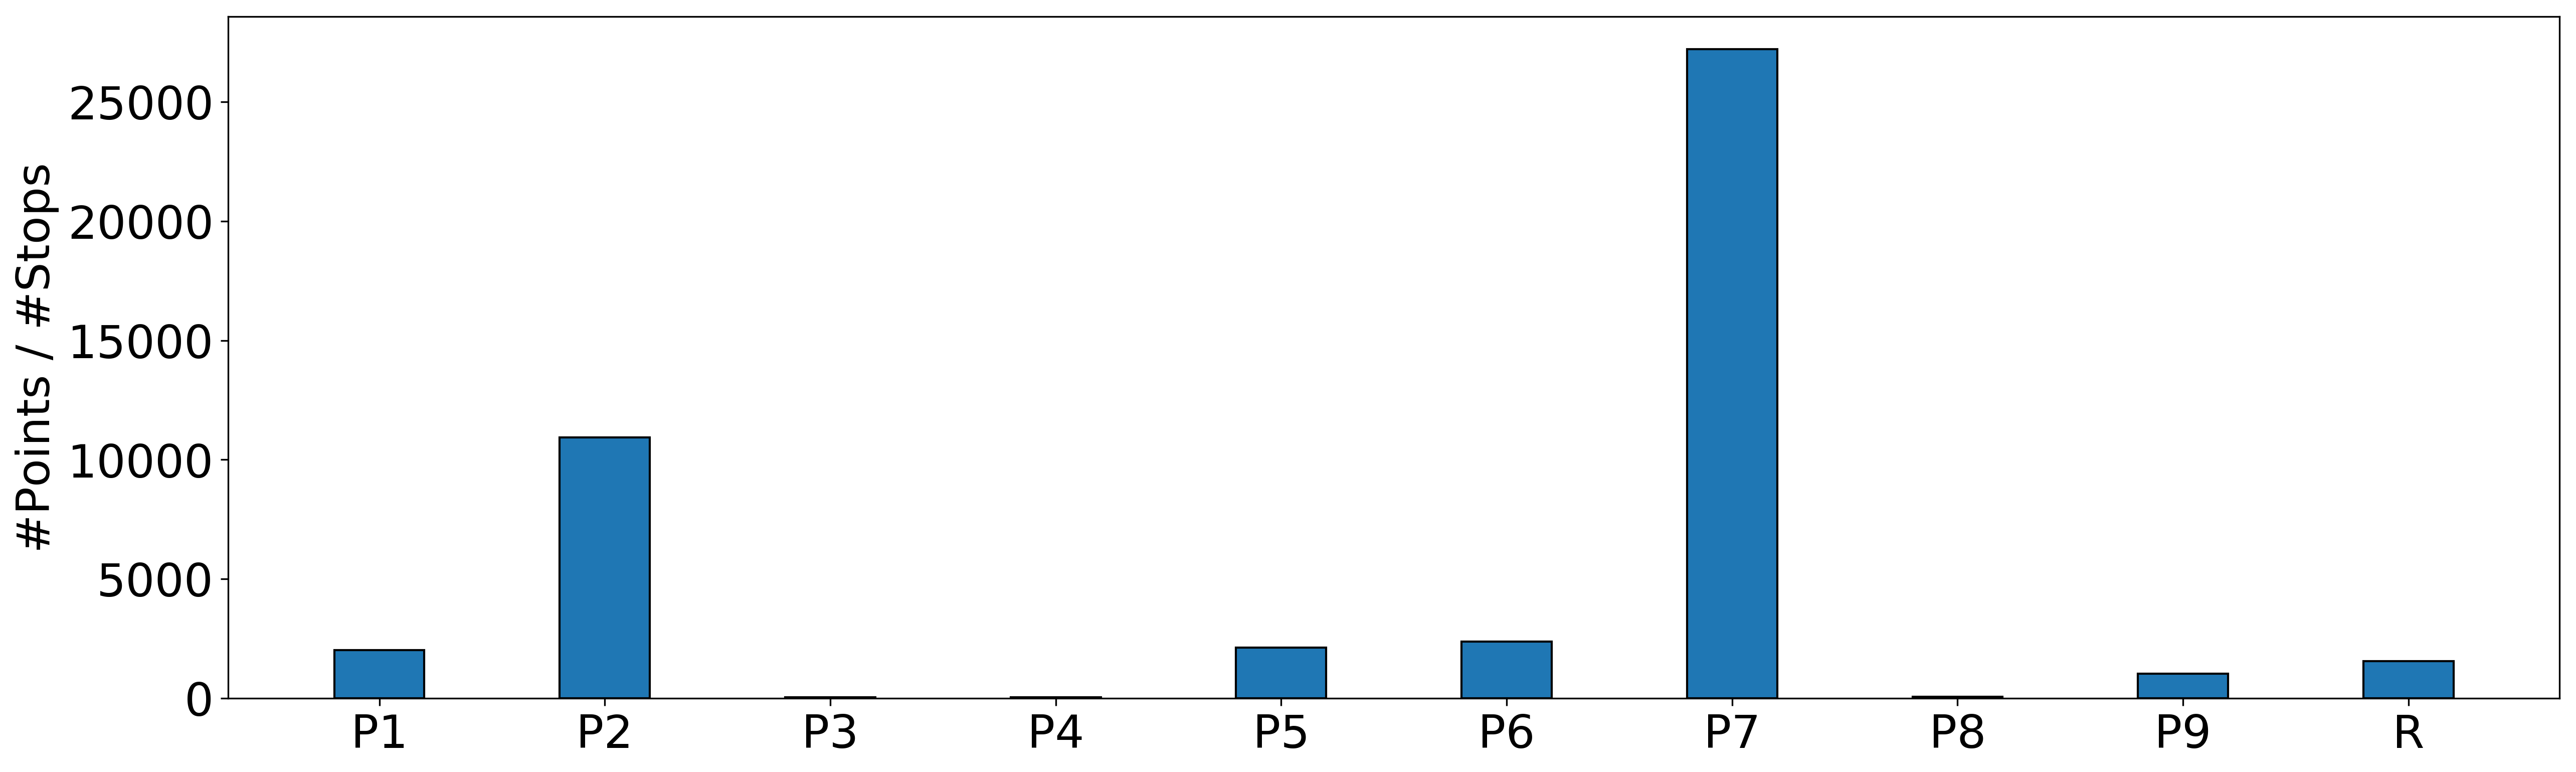
\includegraphics[width=\textwidth]{images/study/storage/compression_N.png}
    \caption{The number of raw location samples (top) and the number of stops (middle) collected, and the ratio between the two, for each participant}
    \label{fig:plot-num-points-stops}
\end{figure}

\begin{figure}
    \centering
    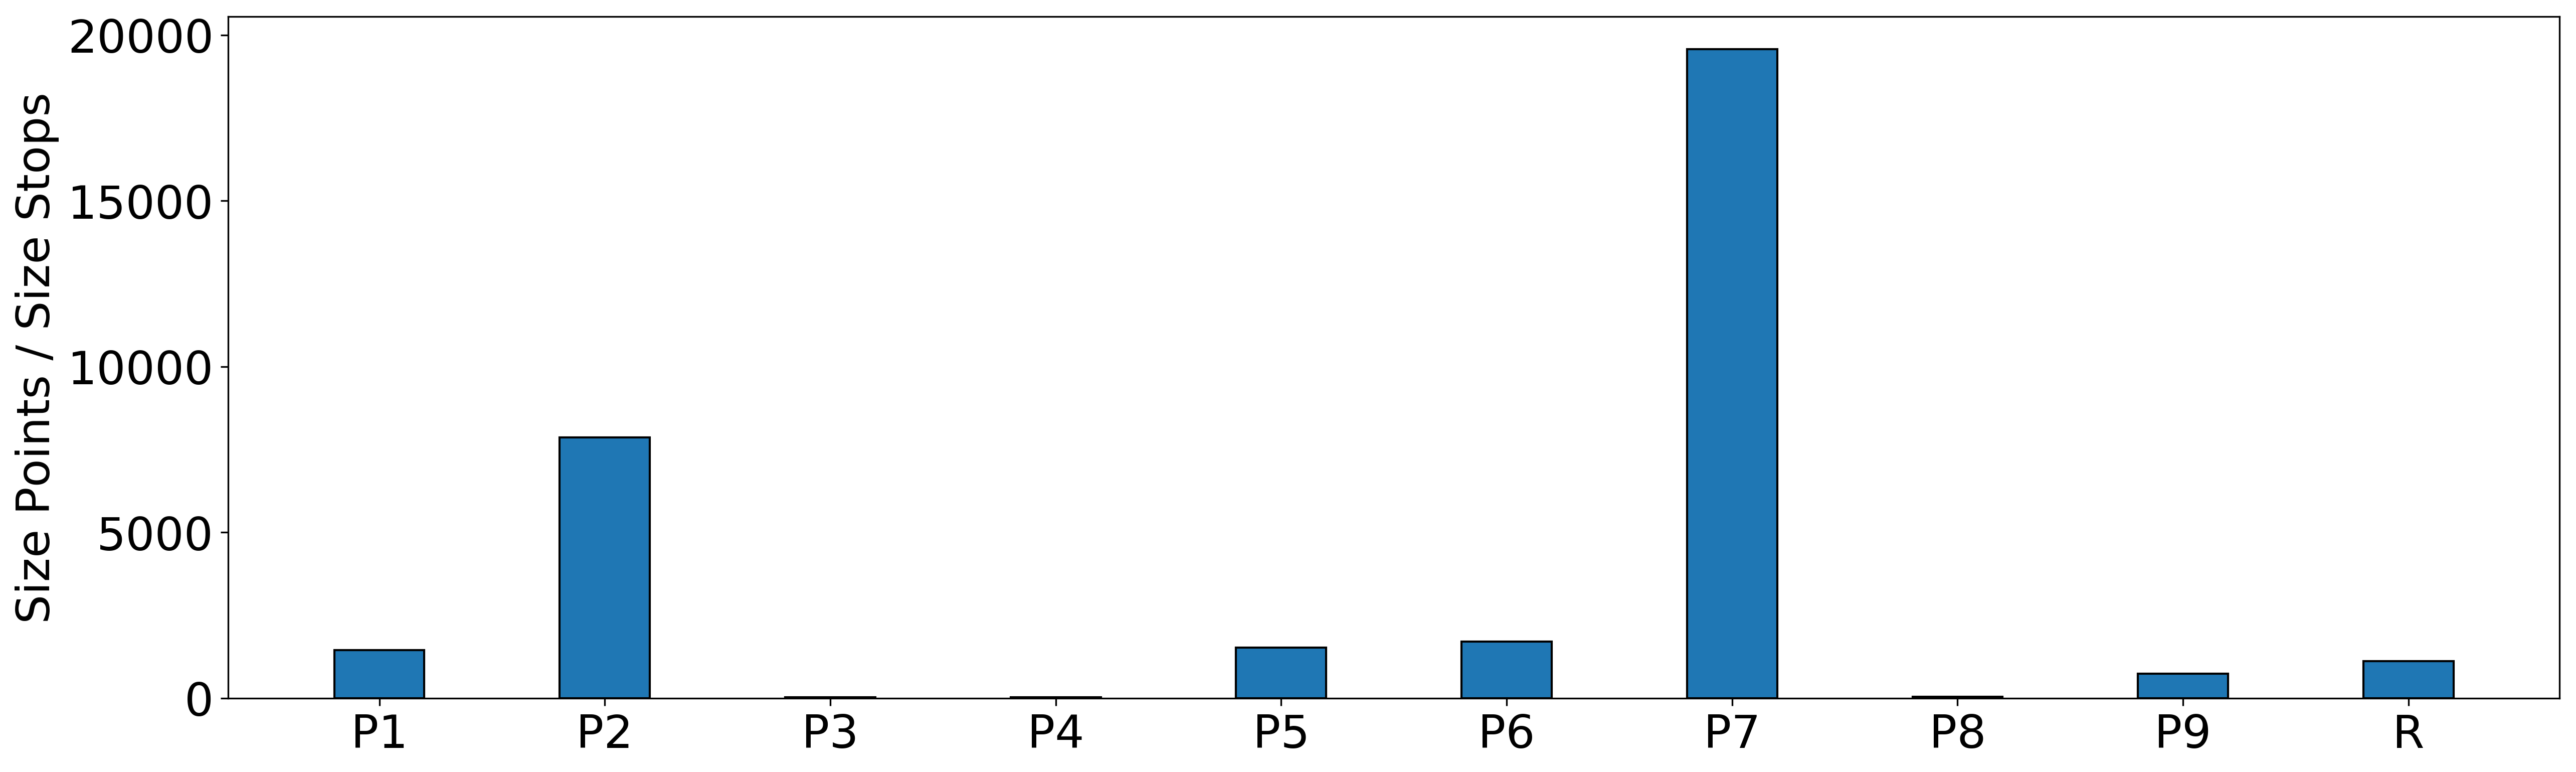
\includegraphics[width=\textwidth]{images/study/storage/compression_mb.png}
    \caption{The ratio between location samples and stops expressed in terms of storage, in MB}
    \label{fig:plot-num-points-stops}
\end{figure}

The average size of a serialized \textit{LocationSample} was compted based on file size to be around 100 bytes, with a stop is being 140 bytes. With this information, it is possible to calculate the compression rate for each participant, i.e. how much their dataset was reduced by converting location samples into stops, and this is shown in Figure \ref{fig:plot-num-points-stops}. The number of valid days for a specific feature is the number of days for which the user gave answers, and the feature could be calculated. If the user for example turned off their phone during the night, the Home Stay feature could not be calculated, but the routine index feature and the number of places will likely still have been calculated.

\subsection{Subjectivity of Answers and Ground Truth}
A thing to keep in mind is that the participants' answers are not ground truth, and there are multiple reasons why a participant's answer may be inaccurate. Firstly, people's subjective recollection is not necessarily as accurate as they think it might me. Secondly, it was not communicated explicitly to the participants what exactly counts as a place, and how their 'routine' is calculated - this means that participants may have filled out the questionnaire differently, given the same ground truth data - for example, whether or not being in the garden counts as being home. Thirdly, some users misunderstood the routine scale, and users whose data looked strange were contacted afterward to enquire about whether they had misunderstood the question, and if so the answers were corrected as much as could be done. Lastly, the hour away from home and routine index answers were very course-grained, and therefore the participants were probably rarely able to give exact answers, according to their own recollection. 

\subsection{Missing Location Data and Answers}
The sampling was set to once per second, yet data was not sampled uniformly. In fact, there were many gaps in the collected data. Figure \ref{fig:plot-gaps-data} shows the data of the author collected during the study over 24 days. The author was very diligent in tracking his location and yet substantial gaps in the data can be observed. These gaps are consistent in the morning where the phone is not moving around, but after 6 AM it seems there is no pattern for the gaps. The event plot for the collected data for particpant P8 is shown  in Figre \ref{fig:p8-gaps} in Appendix \ref{appendix:data-analysis}. \\


\begin{figure}[h]
    \centering
    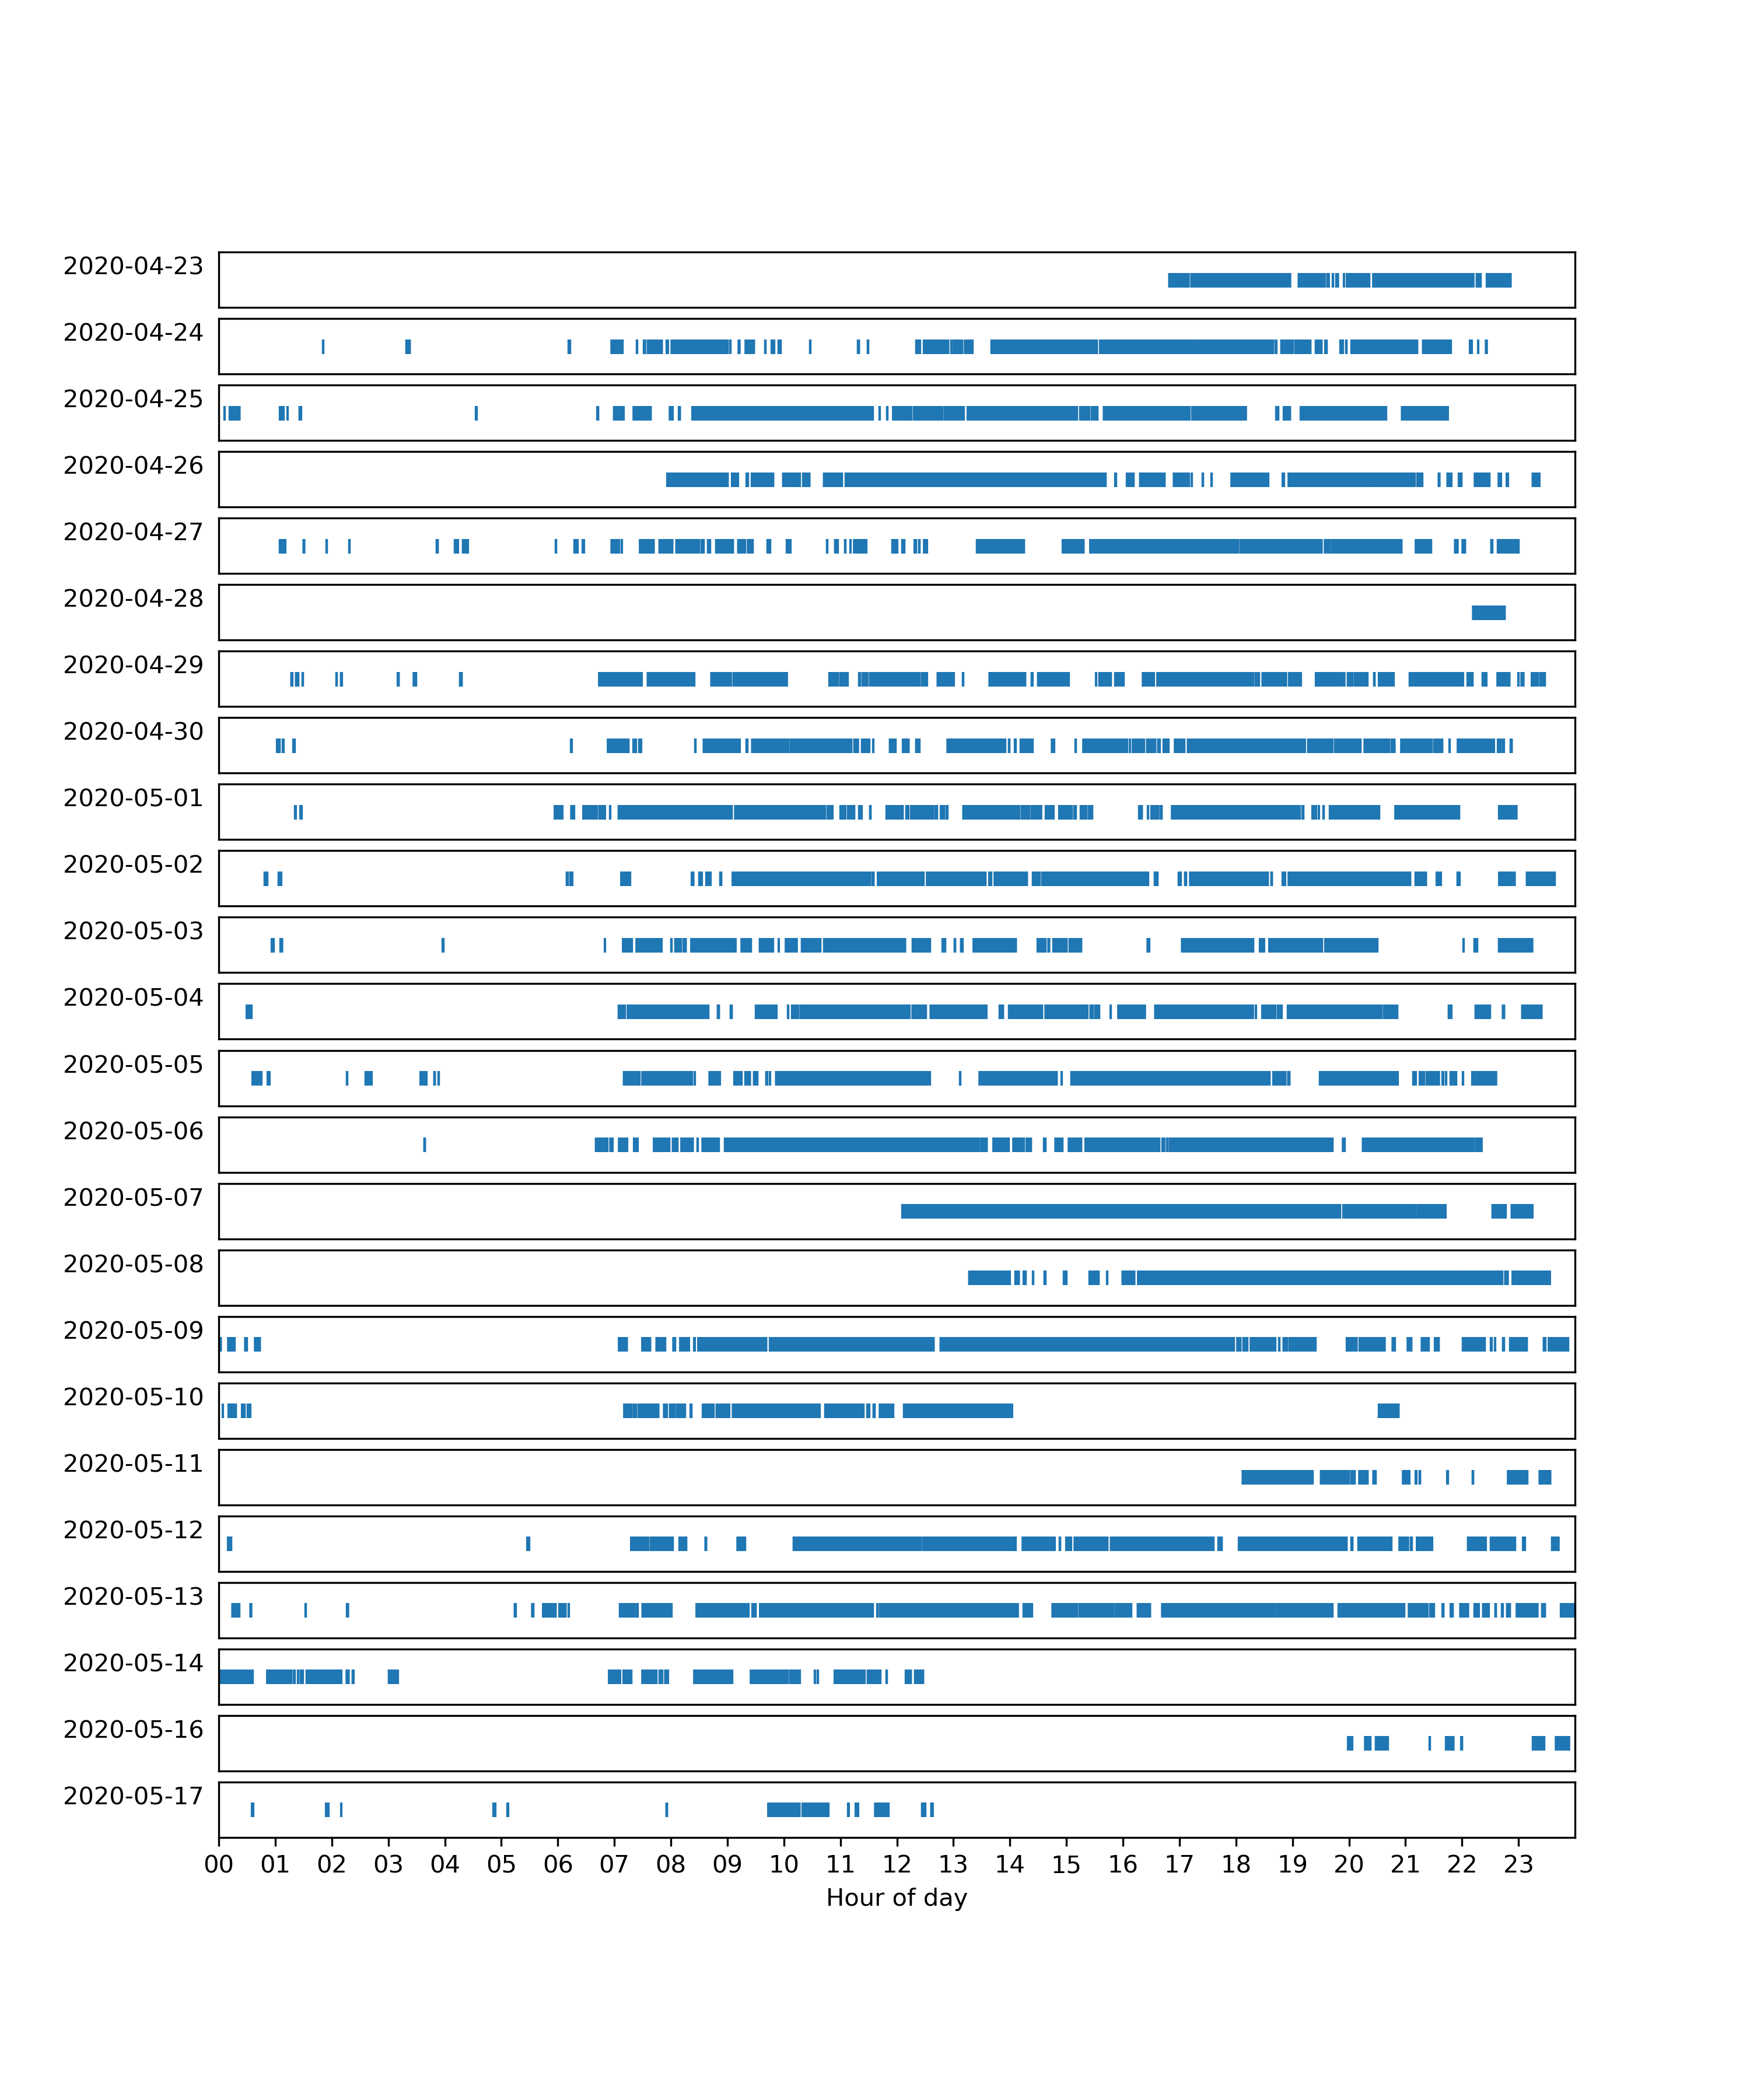
\includegraphics[width=\textwidth]{images/study/thomas-gaps.png}
    \caption{An event plot for the author's sampled location data, each day of the study. As can be seen there are quite a few gaps in the data which will make the computes features less accurate}
    \label{fig:plot-gaps-data}
\end{figure}

Regarding the subjective user data, many users missed filling out the diary on several days. Figure \ref{fig:plot-days-answered} shows the number of total days where a participant participated in the study against the days on which they provided an answer. It was only possible to calculate the error between computed features and the answers on day, if the participant gave an answer. This means that for some participants, a lot of data was thrown away for the data analysis. As an example, it was considered whether or not to entirely get rid of P9 since he/she has very little data both terms of total days collected and even fewer in terms of days with answers. 

\begin{figure}[h]
    \centering
    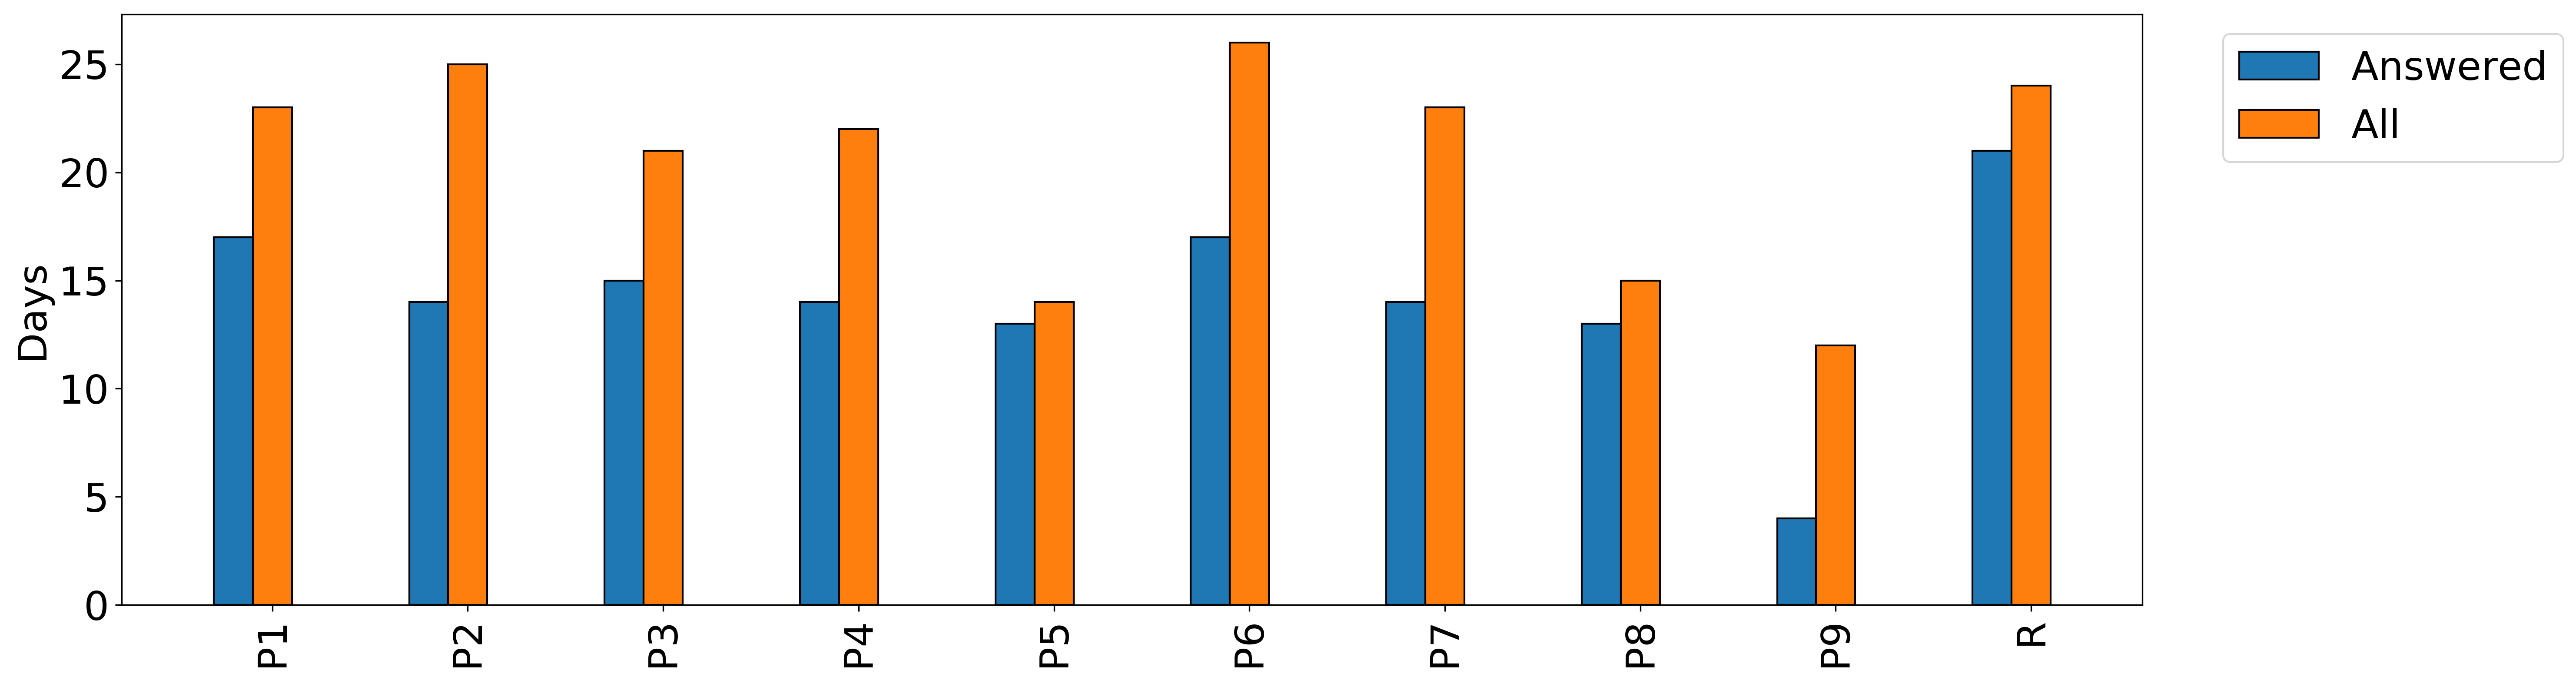
\includegraphics[width=\textwidth]{images/study/storage/answers_days_plot.png}
    \caption{The total number of days of participation vs the days for which the diary was filled out by the participant. As can be seen, some users often forgot to give an answer}
    \label{fig:plot-days-answered}
\end{figure}

Another problem that was encountered was when participants would fill out the questionnaire during the night, or the very next morning due to forgetting the previous evening. This meant the answer for day $n$ would be listed as date $n+1$, i.e. the wrong date. This was rectified by changing all answers given between 00:00 and 10:00 to the previous date at 23:59:59. In addition, some users entirely forgot certain days but remembered it the following day, and reported it manually to the researcher, and these answers were then added manually. 

\subsection{Feature Evaluation}
The Home Stay feature required the participant to track their location during the night, as previously mentioned. This meant that if they did not, the Home Stay feature could not be evaluated for that particular day, however other features might still be available for computation, such as the Number of Places. This meant that the number of days for which a given feature can be compared to the answers is not necessarily the same for all features. 

\begin{figure}[h]
    \centering
    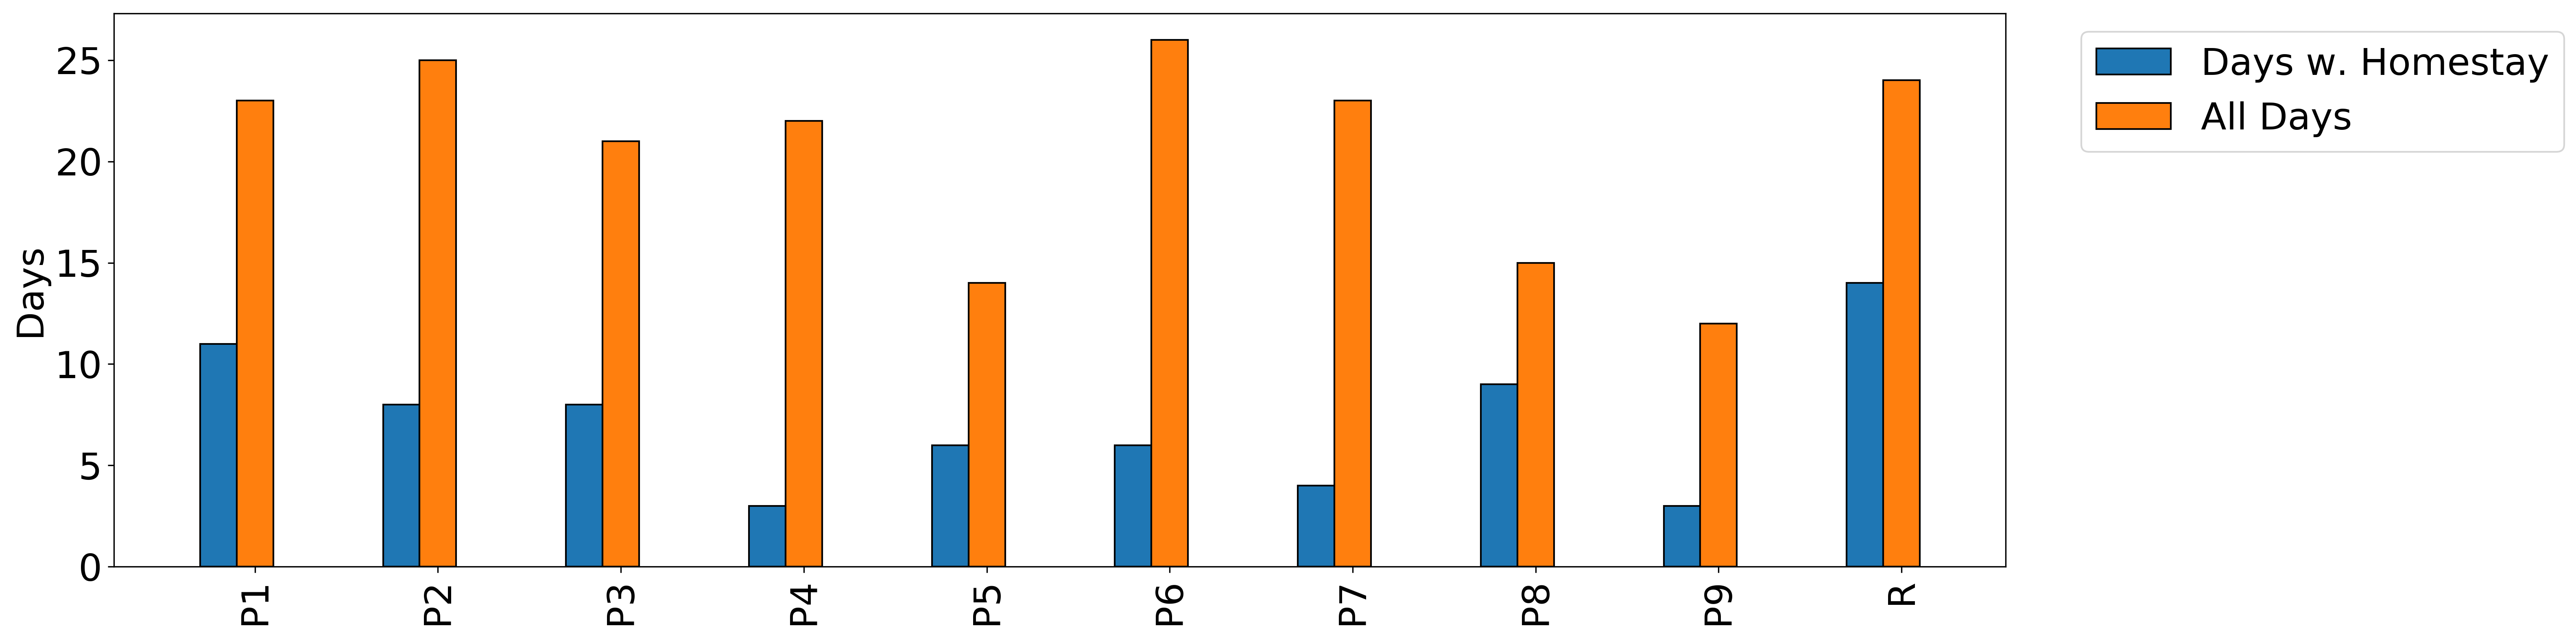
\includegraphics[width=\textwidth]{images/study/homestay_valid_days.png}
    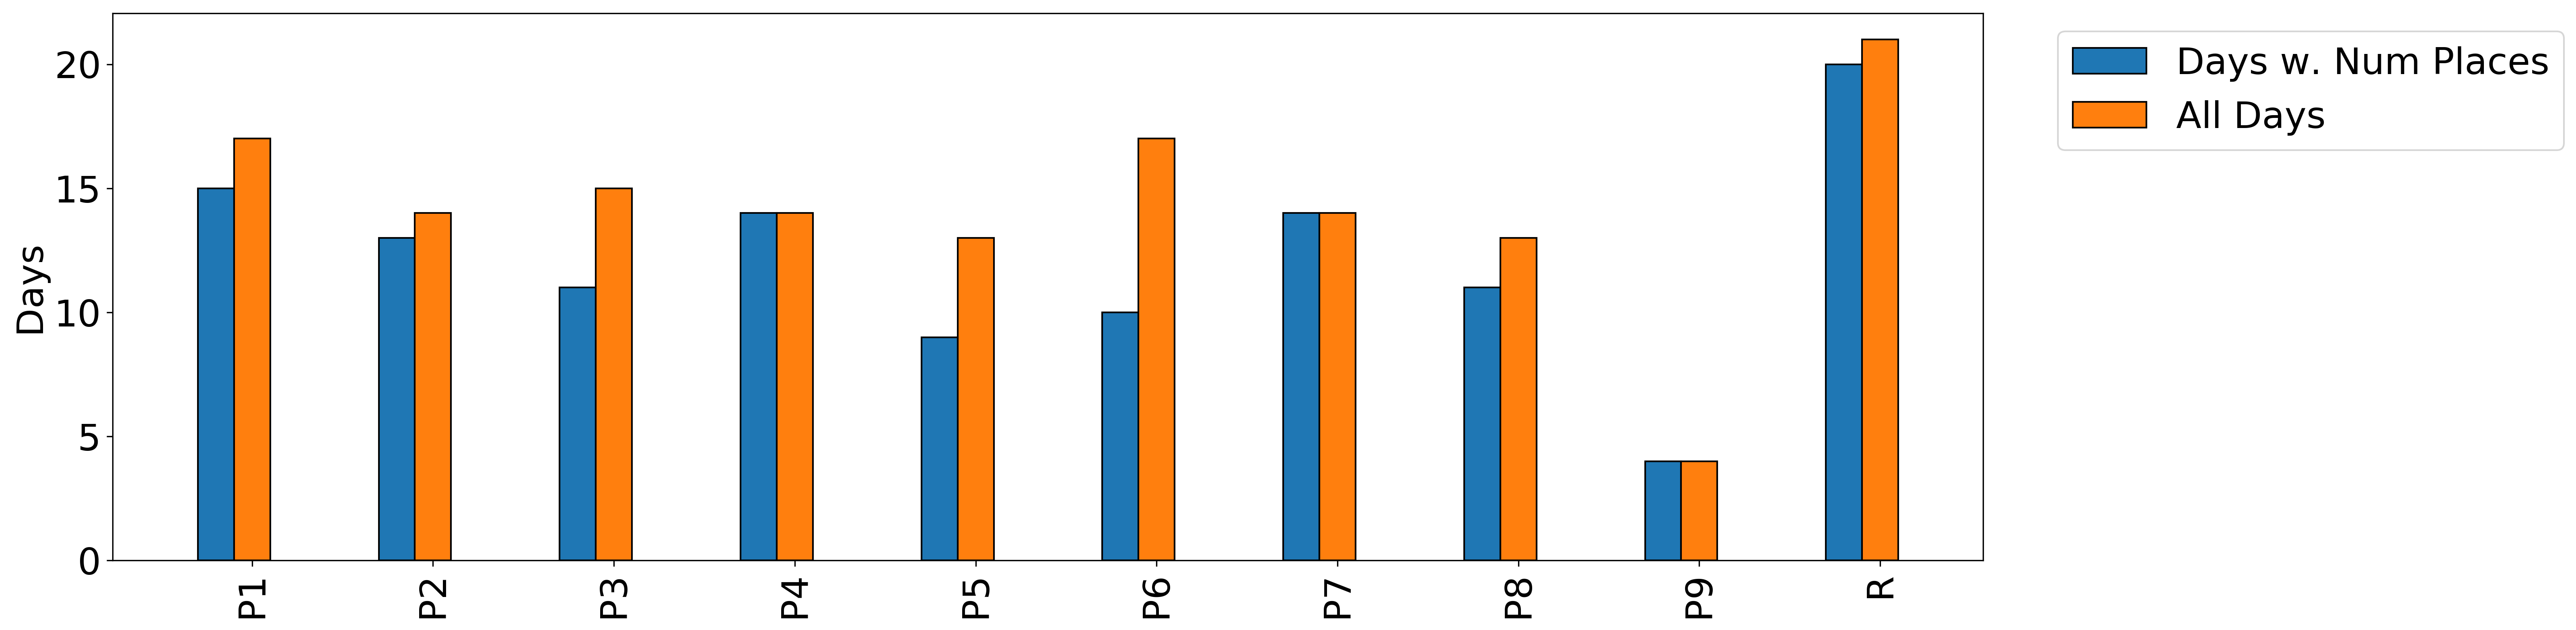
\includegraphics[width=\textwidth]{images/study/numplaces_valid_days.png}
    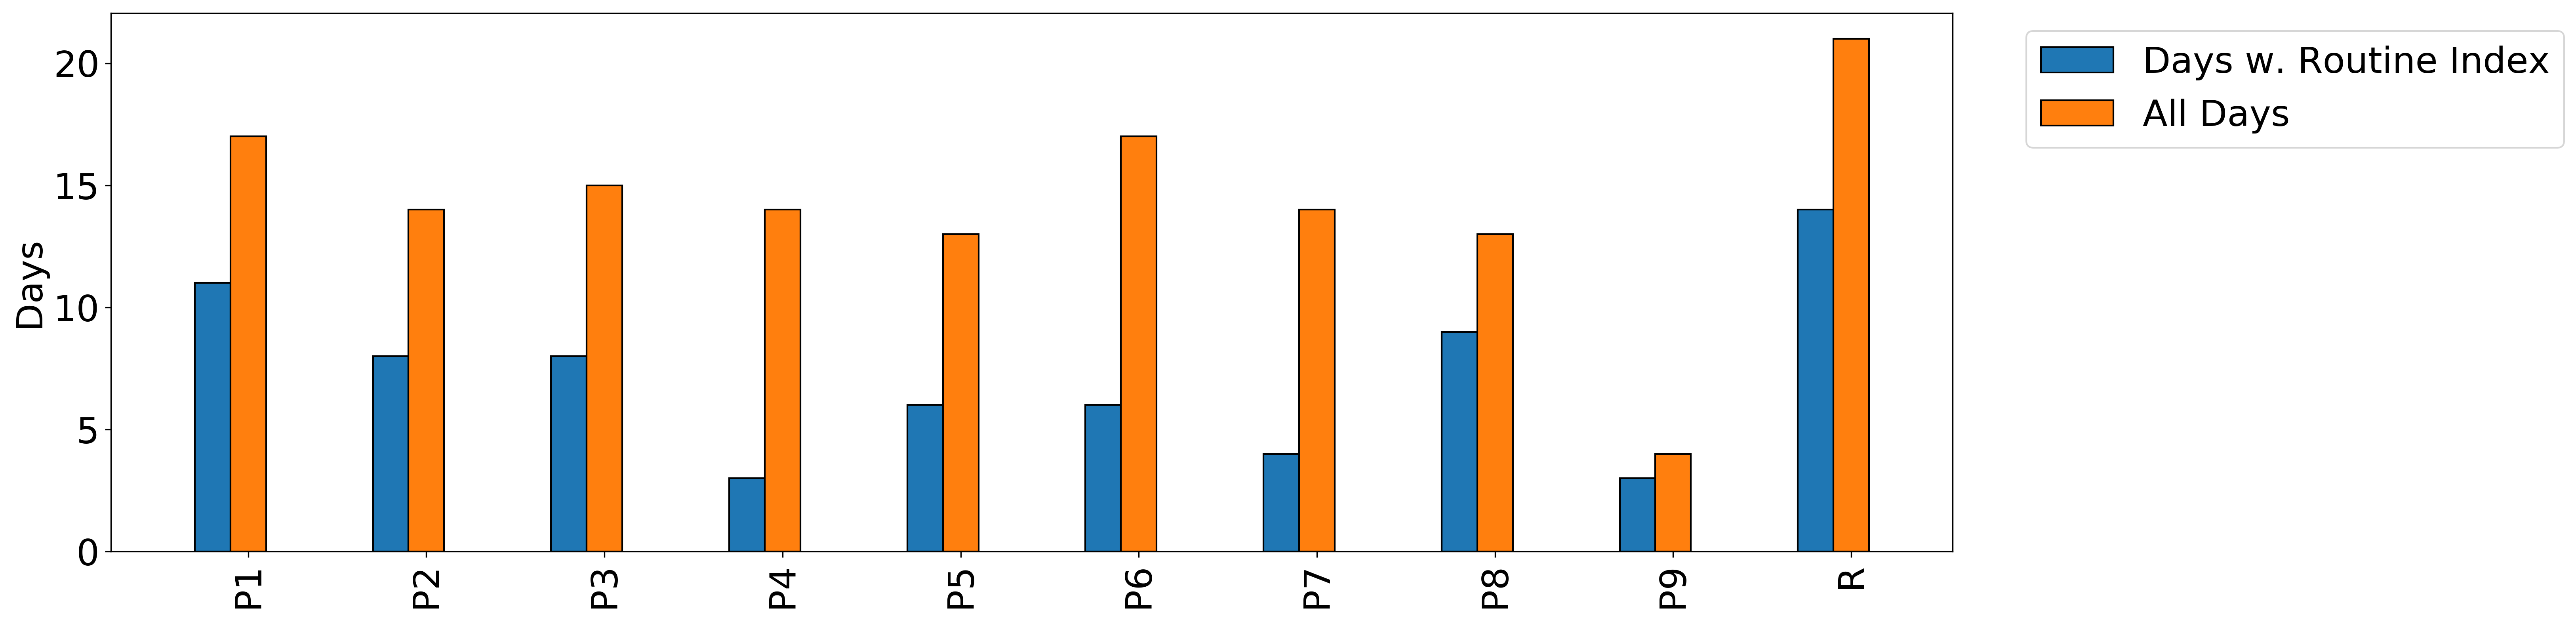
\includegraphics[width=\textwidth]{images/study/routine_valid_days.png}
    \caption{The days for which a given feature could be evaluated, out of the total days for which an answer was given and features were computed. As can be seen from the top plot, participant P4 had very few days where the home stay could be computed in comparison to the total number of days tracked which are above 20}
    \label{fig:plot-daily}
\end{figure}

The Home Stay feature is calculated by using the \textit{tracked} time at home, divided by the total time elapsed since midnight, and therefore a small gap in the data will make the feature undershoot. It is therefore to be expected that this feature will lie somewhat lower than the answer given by the user since there will be gaps in the data. 

\begin{figure}[h]
    \centering
    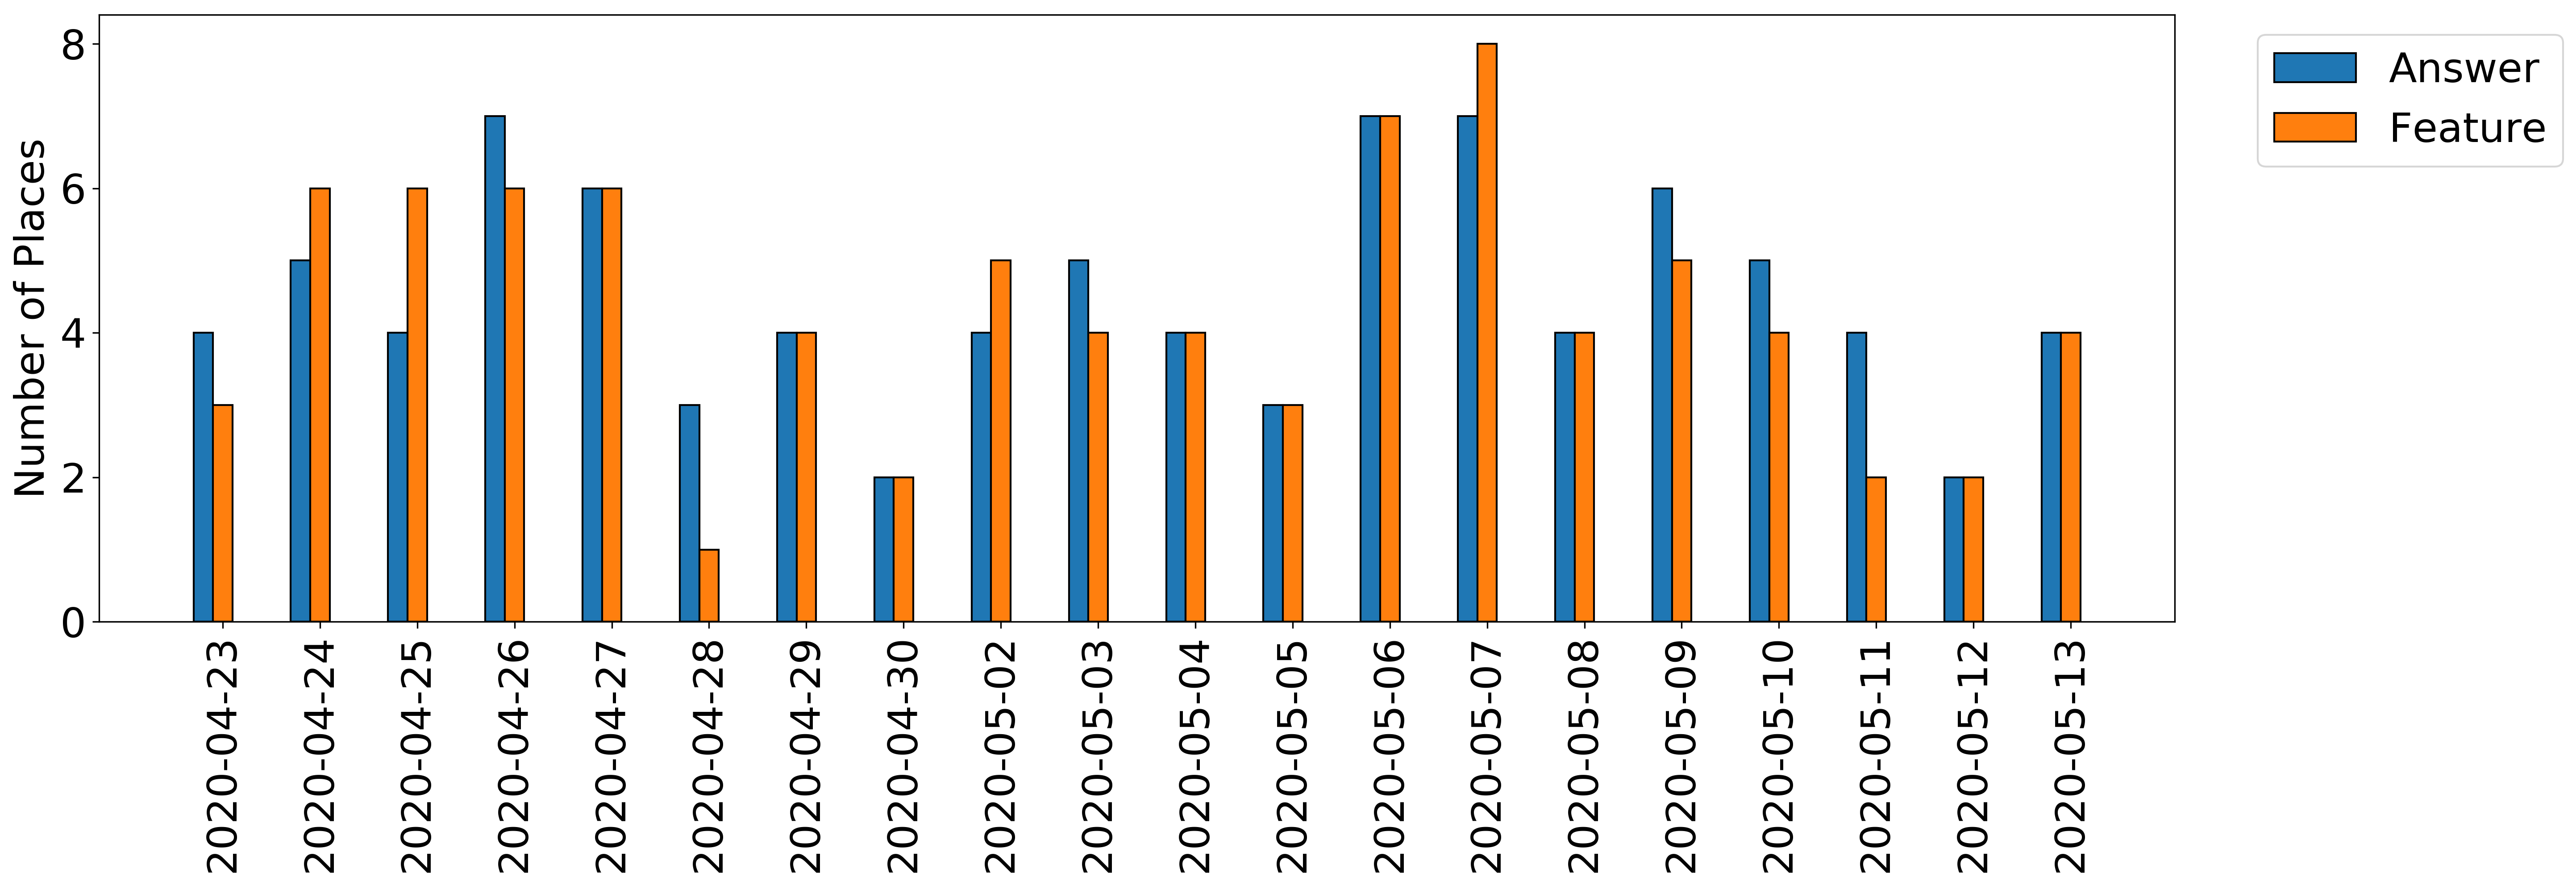
\includegraphics[width=\textwidth]{images/study/places_d6b2d9b9-398b-4e0d-b52b-224747f515c8.png}
    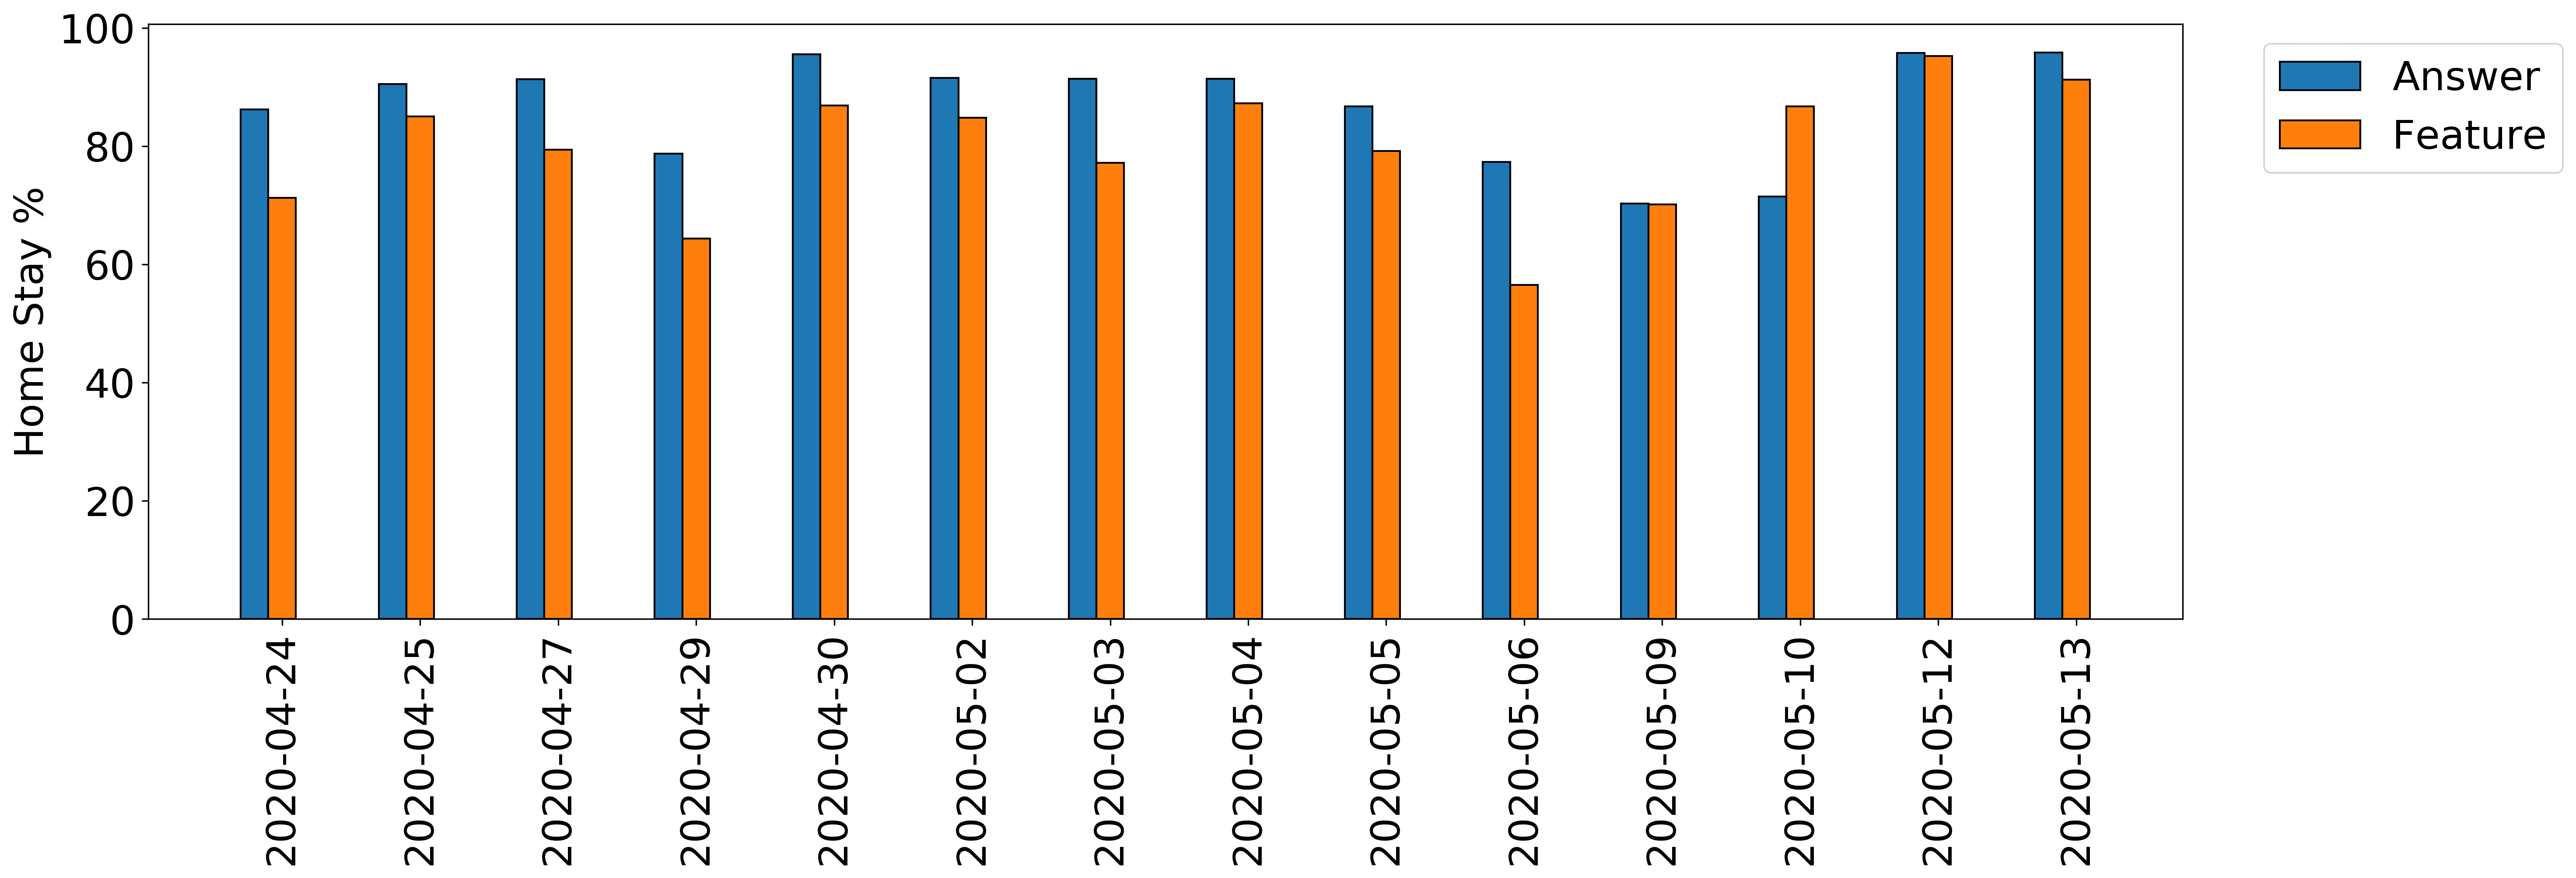
\includegraphics[width=\textwidth]{images/study/homestay_d6b2d9b9-398b-4e0d-b52b-224747f515c8.png}
    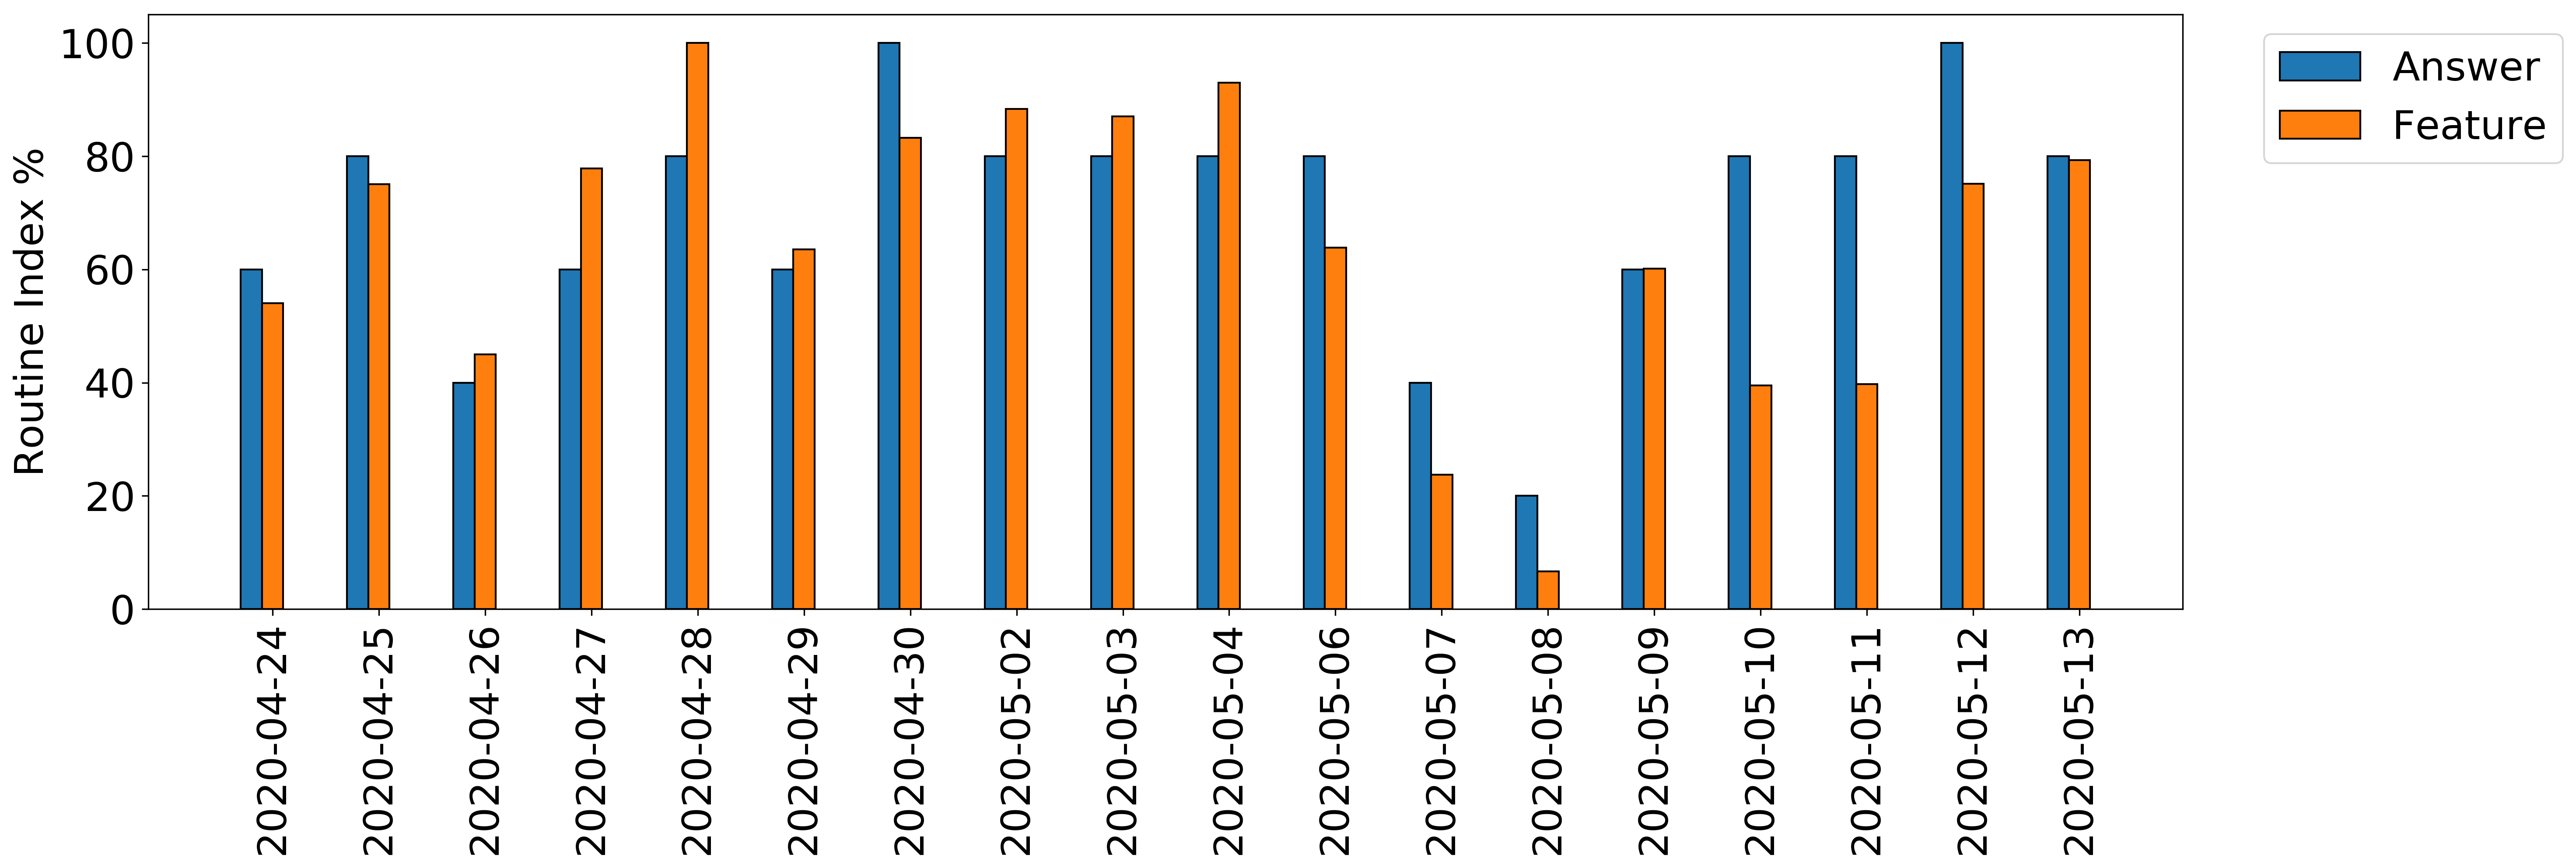
\includegraphics[width=\textwidth]{images/study/routine_d6b2d9b9-398b-4e0d-b52b-224747f515c8.png}
    \caption{The answered and calculated data for each day, for the author}
    \label{fig:plot-author-features}
\end{figure}

The day-by-day results for the author are displayed in figure \ref{fig:plot-daily} and from this plot, the computed features have a high correspondence with the provided answers. However, the feature computation is based on the author's own definitions which mean the computed features and answers of the author are also expected to be highly correlated. It is therefore relevant to show another participant, namely participant P8, who was very diligent in answering and tracking their location data. For this participant, very promising results were also produced which can be seen in Figure \ref{fig:plot-p8-features}.

\begin{figure}[h]
    \centering
    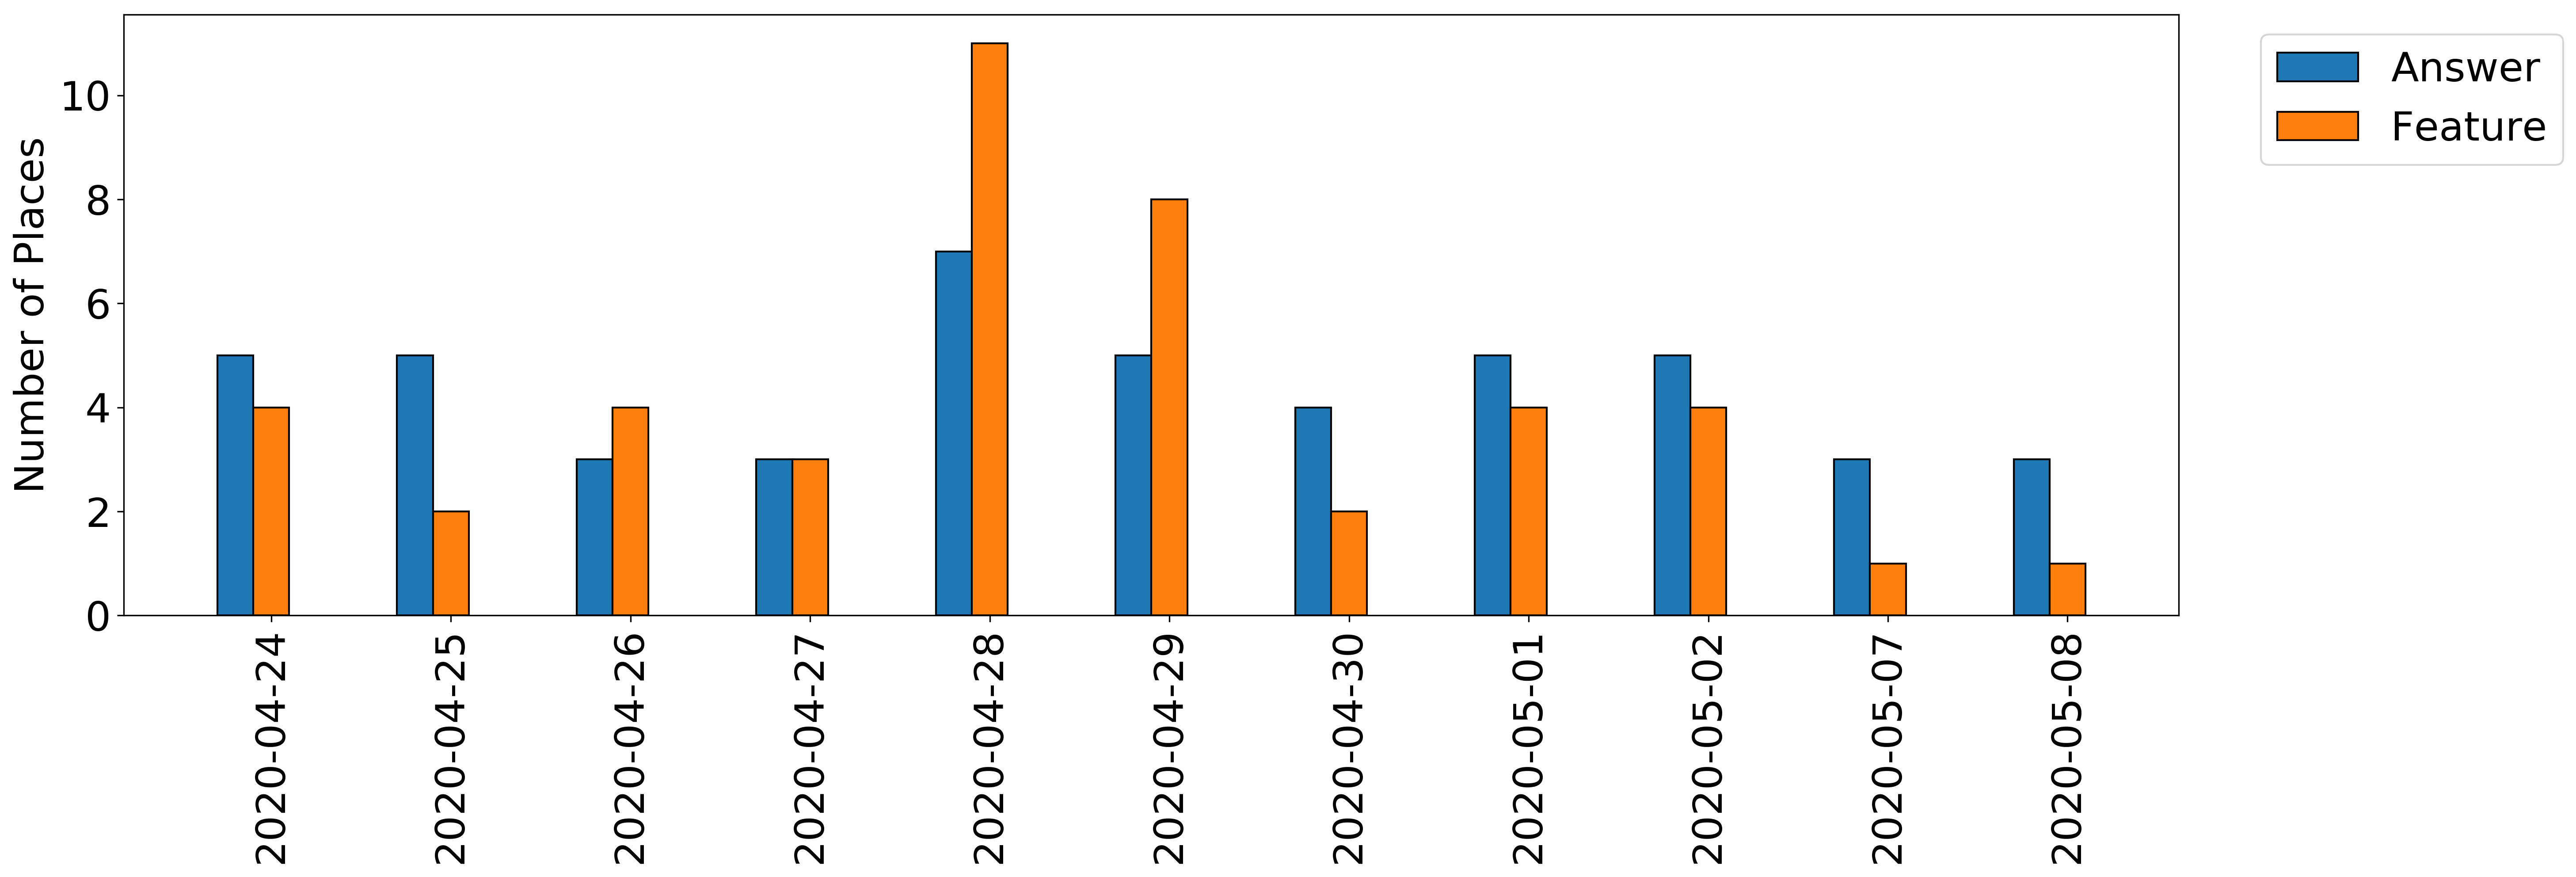
\includegraphics[width=\textwidth]{images/study/places_ec110976-0192-436d-b451-4f5dd97e71d8.png}
    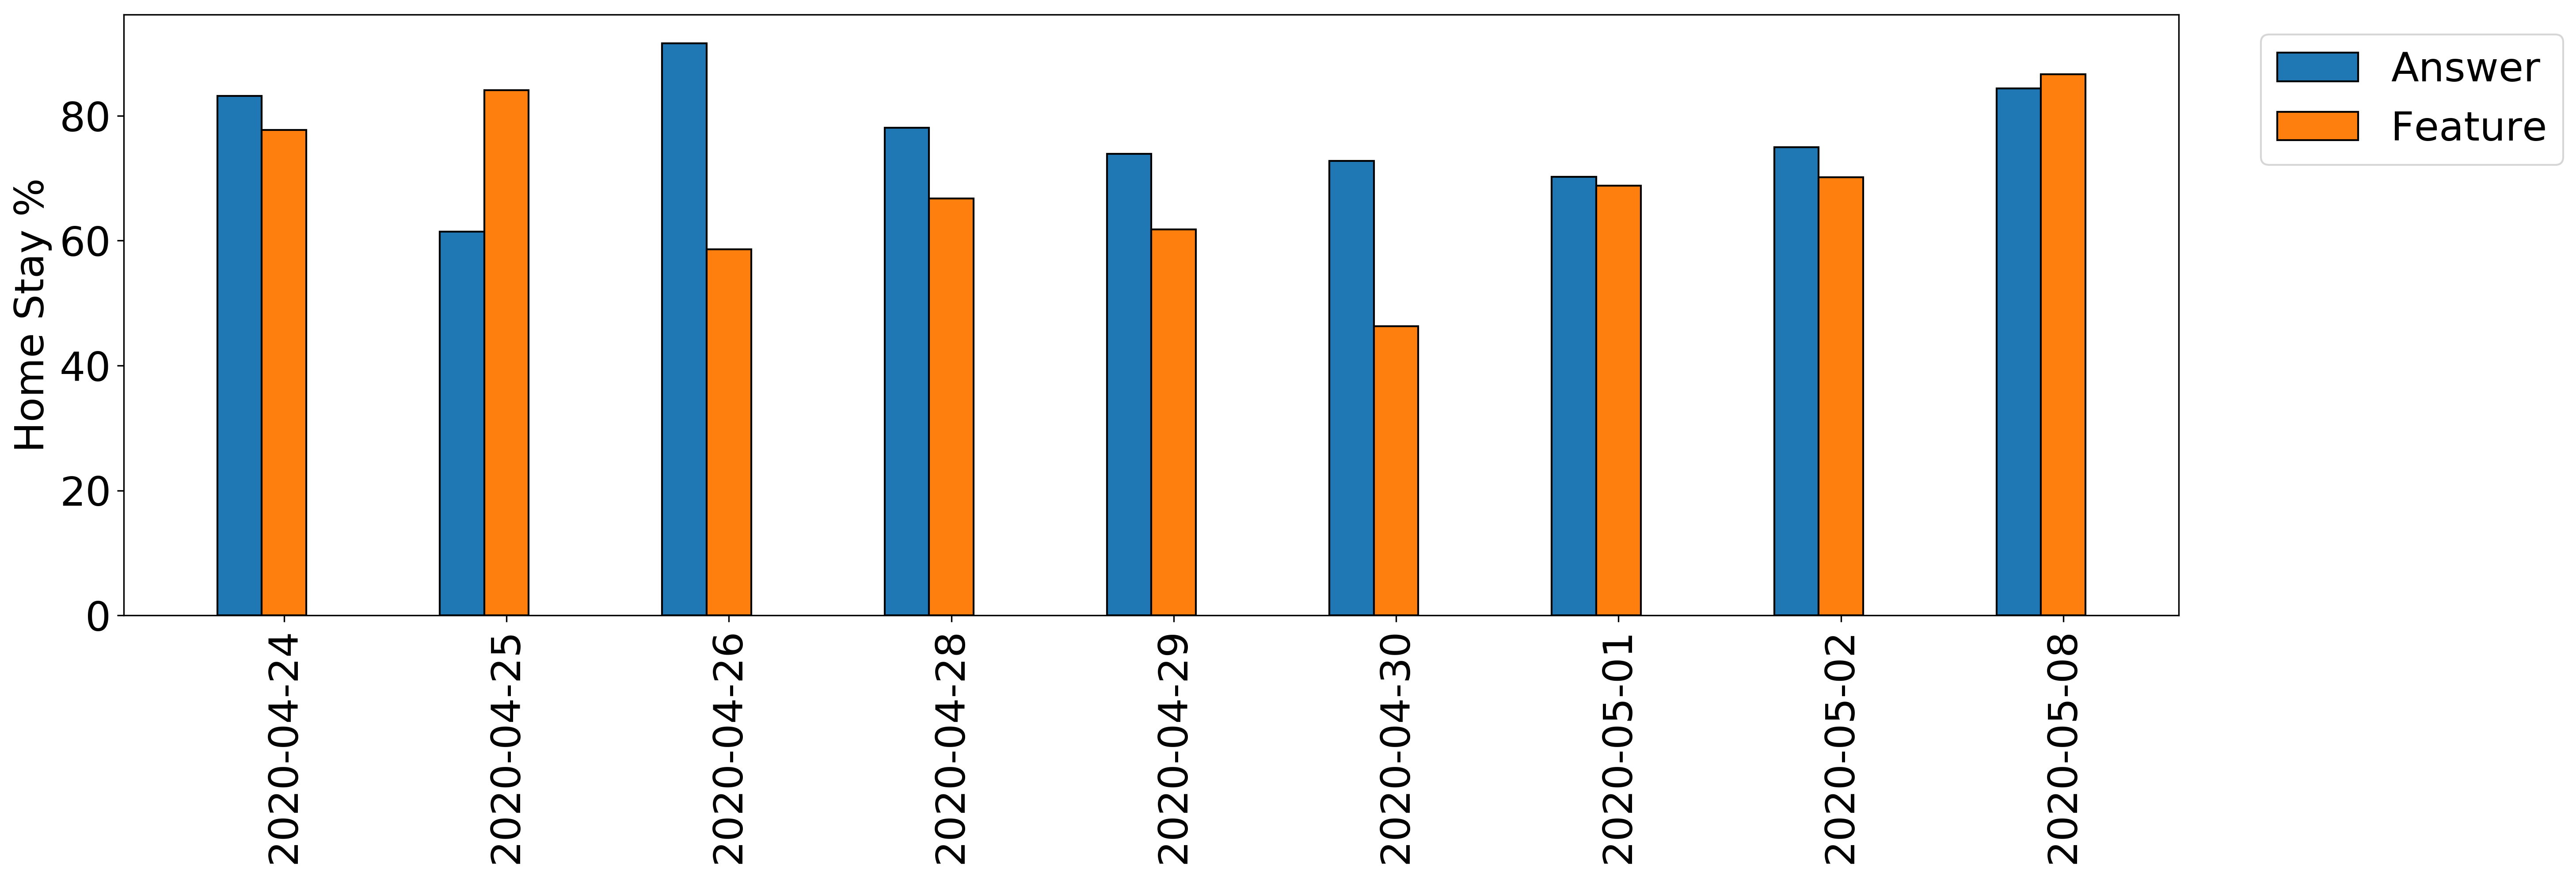
\includegraphics[width=\textwidth]{images/study/homestay_ec110976-0192-436d-b451-4f5dd97e71d8.png}
    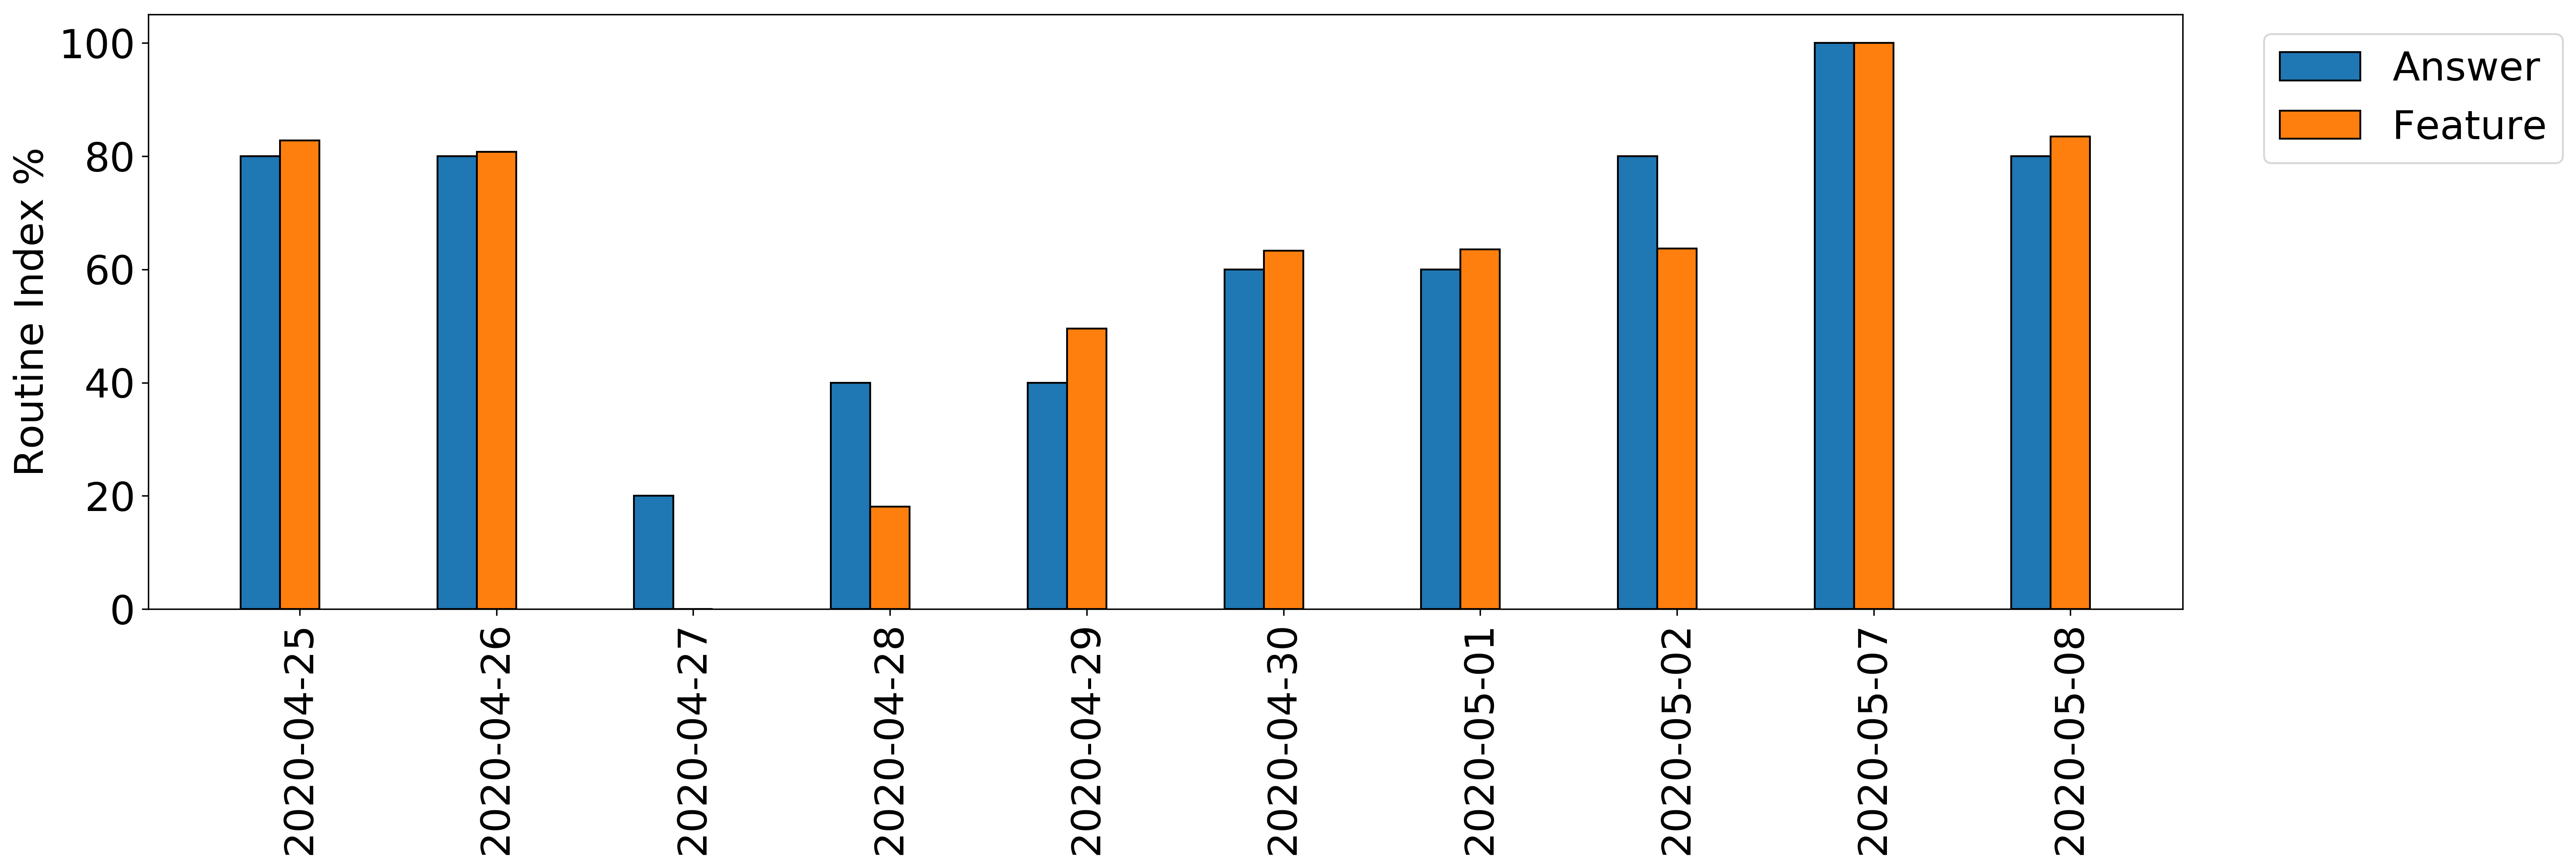
\includegraphics[width=\textwidth]{images/study/routine_ec110976-0192-436d-b451-4f5dd97e71d8.png}
    \caption{The answered and calculated data for each day for participant P8}
    \label{fig:plot-p8-features}
\end{figure}


\subsection{Measuring Errors}
There are a few ways data errors can occur:

\begin{itemize}
    \item The computed feature can be wrong due to gaps in the data (\textit{data collection error})
    \item The subjective answer from the user is wrong, e.g. if they misunderstood the concept of the question (\textit{answer error})
    \item Both of a \textit{data collection error} and an \textit{answer error} are made at the same time
\end{itemize}

Given this can occur, the RMSE was still computed for all three features across participants is shown in Table \ref{tab:error-table}. We observe the following:

\begin{itemize}
    \item The Number of Places predicted deviates with almost 1 place daily.

    \item The Home Stay percentage deviates with 14\% daily.

    \item The Routine Index deviates with 22.5\% daily. Here it is important to note than the Routine Index answer was given on scale with 20 percent increments which means that the 22.5\% RMSE is equivalent to one 'step' one the scale.
\end{itemize}

\begin{table}[]
    \centering
    \begin{tabular}{|l|l|l|l|}
    \hline
                        & \textbf{Number of Places} & \textbf{Home Stay} & \textbf{Routine Index} \\ \hline
    \textbf{Mean RMSE}       & 0.99                      & 14.27 (\%)         & 22.5 (\%)              \\ \hline
    \end{tabular}
    \caption{The mean RMSE computed for all participants}
    \label{tab:error-table}
\end{table}


To say something about whether or not the features undershoot or overshoot, the mean error was calculated for each participant as as $ME = \frac{\sum(F) - \sum(A)}{N}$ (where $N$ is the total number of days for the specific feature, for the participant). If the mean error is positive, the feature overshoots compared to the answered value, and vice versa if the error is negative. Since the mean error has a sign, i.e. either positive or negative, the 'mean' mean error cannot be computed. Instead, the individual mean error for each participant is plotted in Figure \ref{fig:plot-mean-error}. From this figure we observe the following:

\begin{itemize}
    \item The Number of Places feature undershoots by around 0.6 places or lower for most participants, with P7 being an outlier with -1.5 places. It is likely that the undershooting stems from \textit{data collection errors}, which can lead to places not being detected.

    \item The Home Stay feature undershoots for 8/10 participants, most of these having an error under 10\%. For those two participants where the feature overshoots, the error is also within 10\%. It is highly likely that the undershooting stems from \textit{data collection errors} leading to an underestimation of the time spent at home.

    \item The Routine Index feature is mixed with an equal number of participants for which it overshoots and undershoots. The current implementation of the feature will ignore time-slots for which data is missing, which leads to the Routine Index overshooting if a lot of data is missing. This feature is likely affected both by \textit{data collection errors} as well as \textit{answer errors}, hence the varying results.
\end{itemize}

\begin{figure}[h]
    \centering
    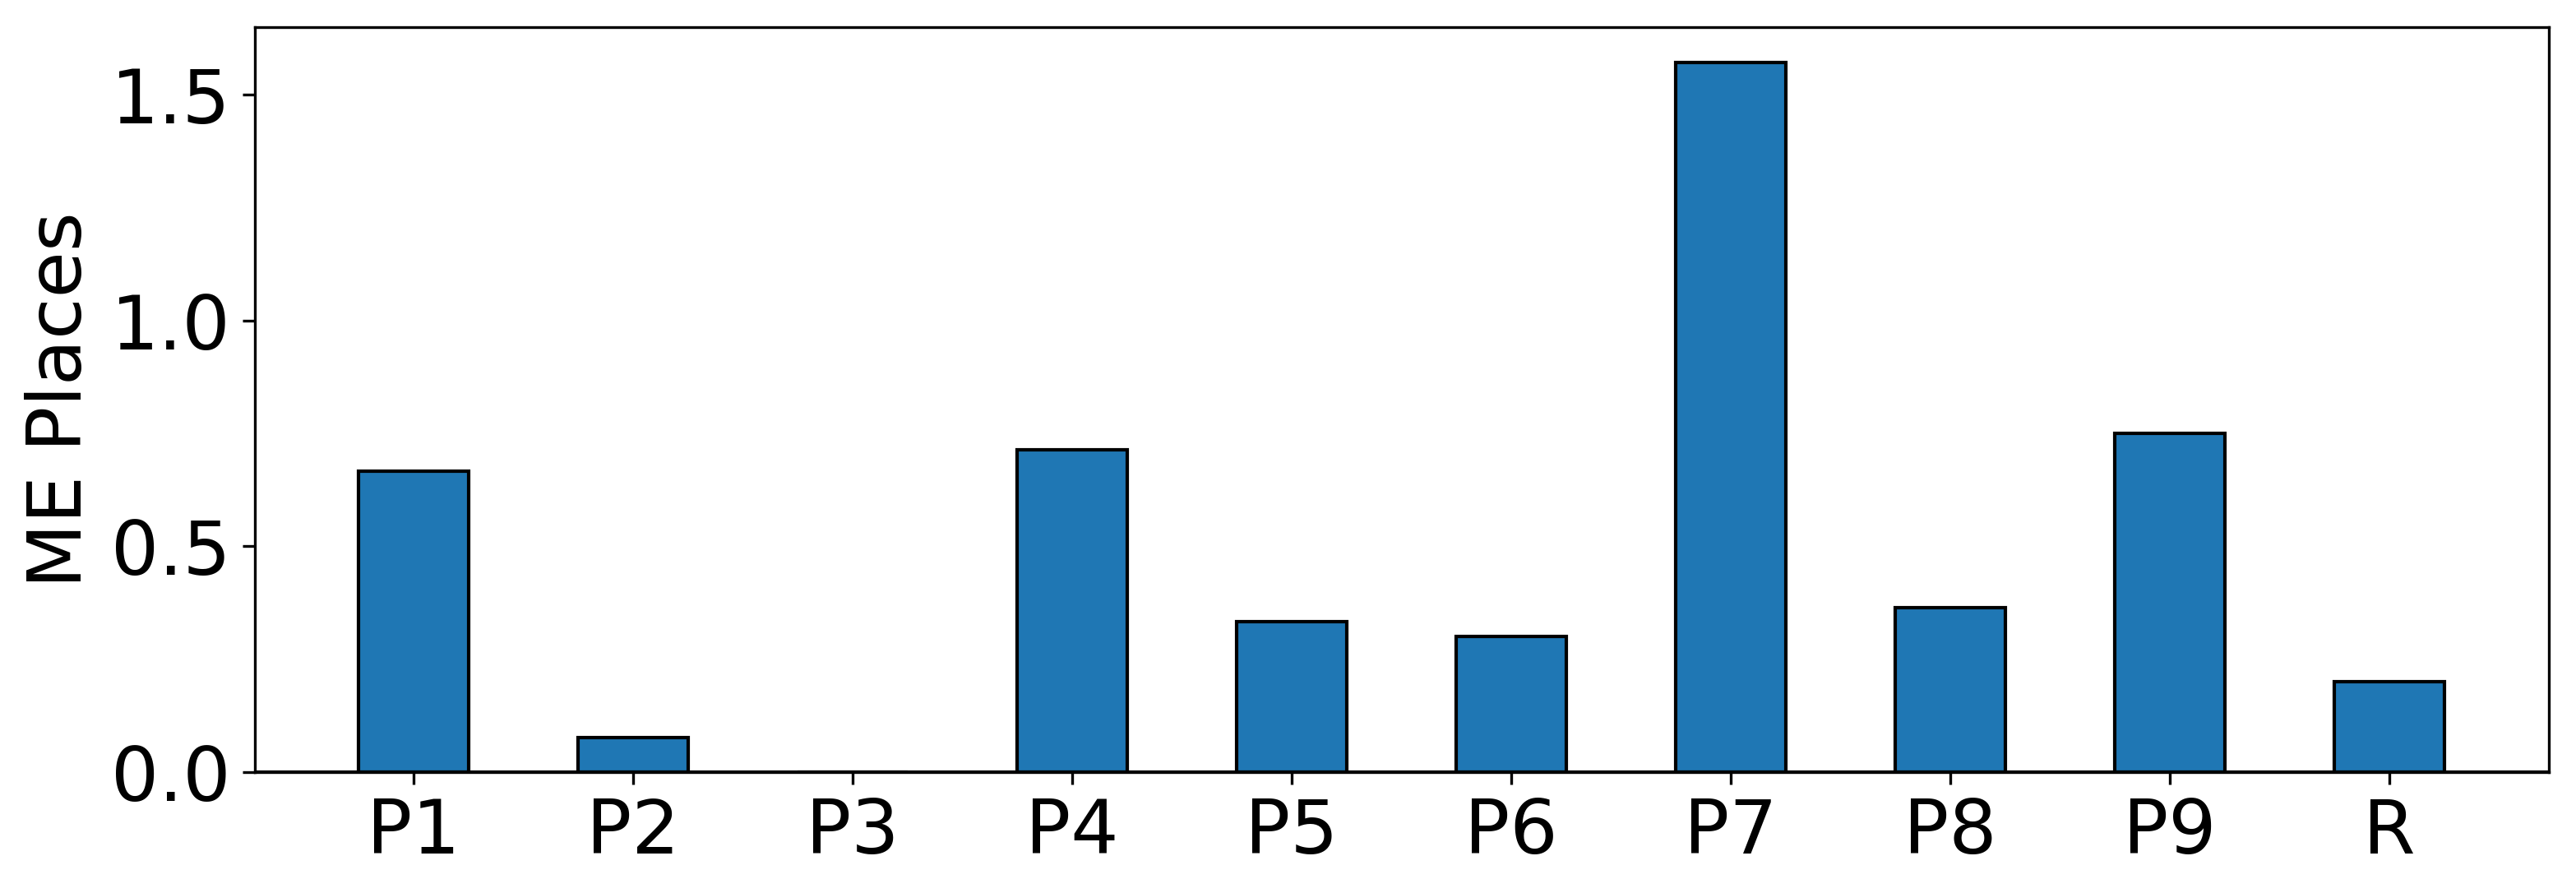
\includegraphics[width=\textwidth]{images/study/me_places.png}
    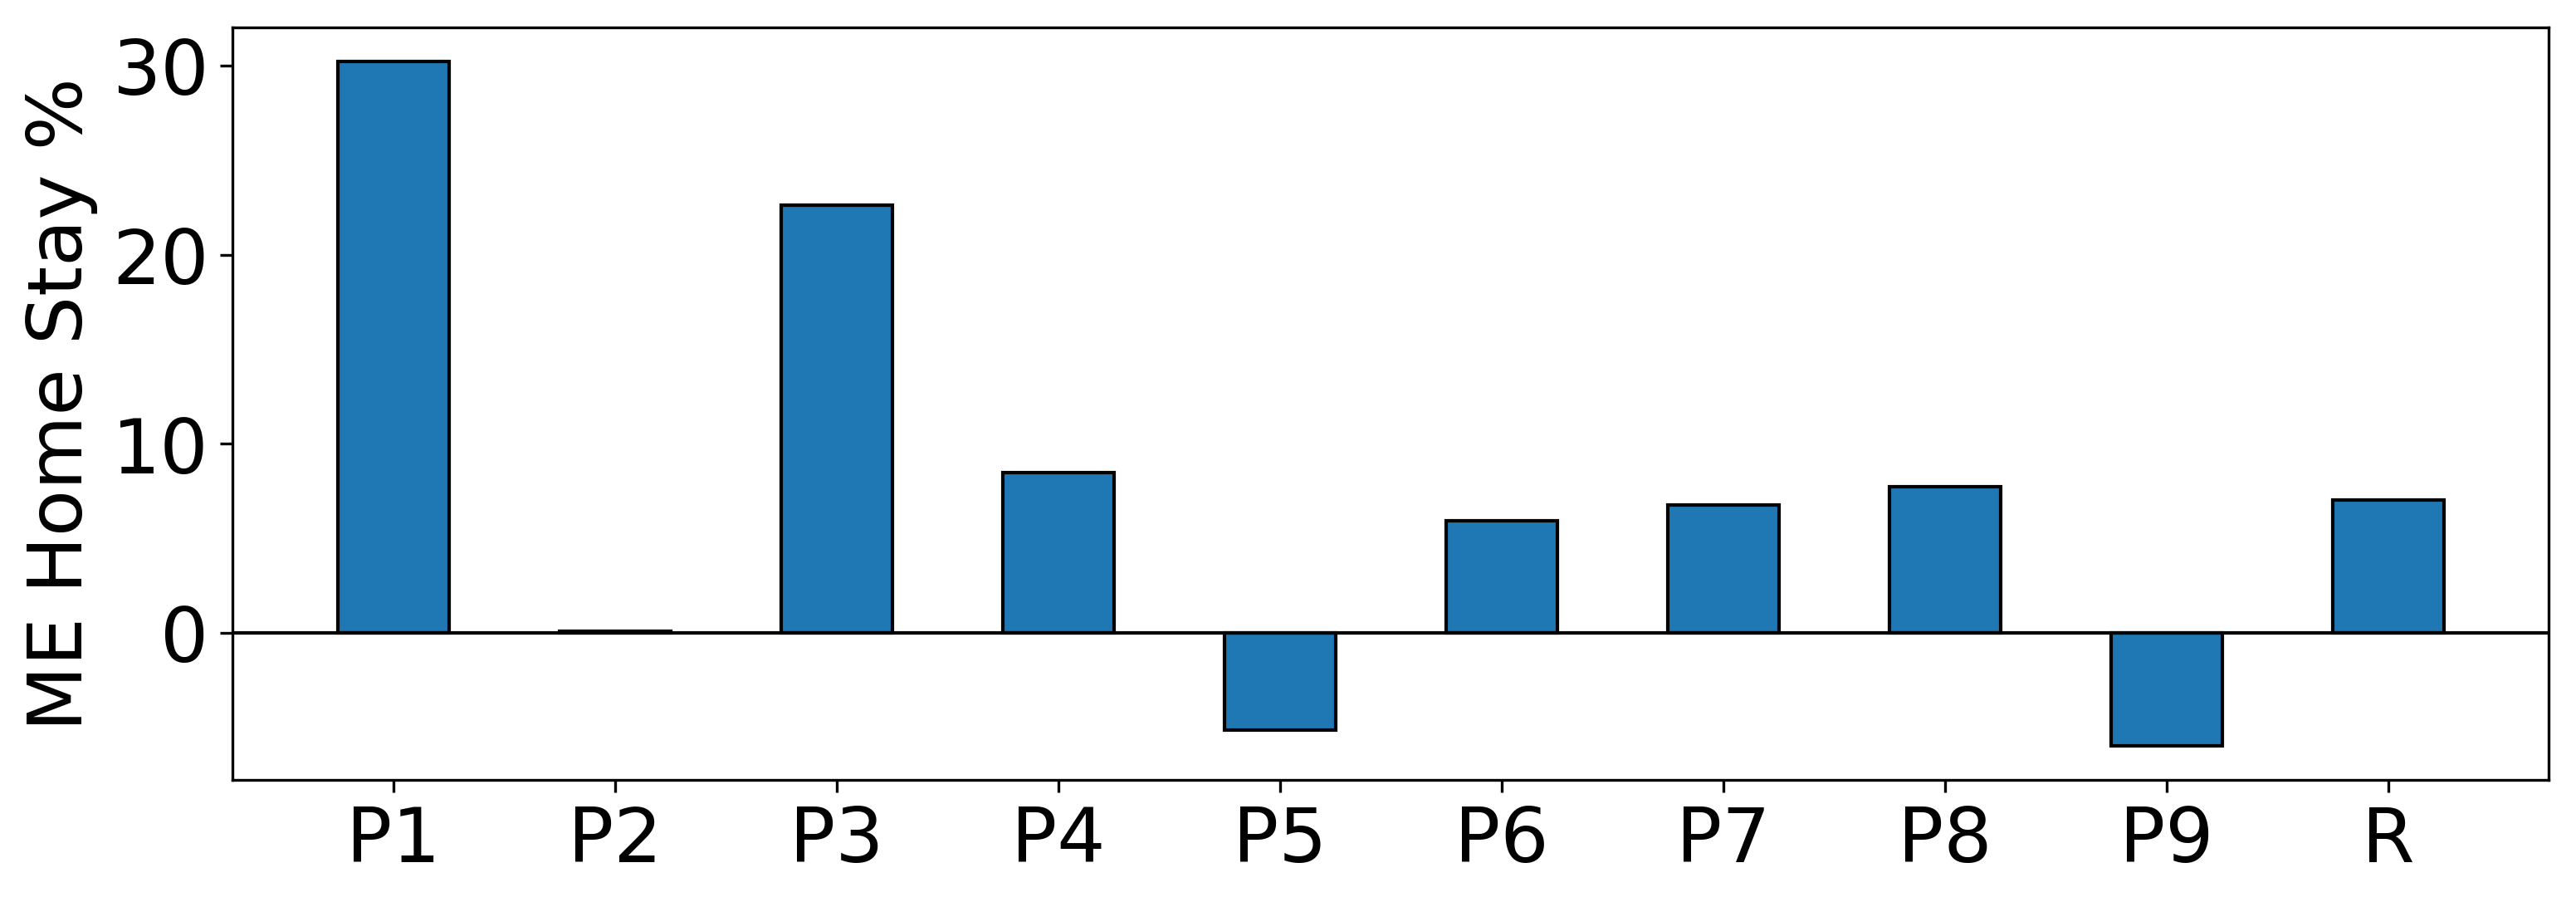
\includegraphics[width=\textwidth]{images/study/me_homestay.png}
    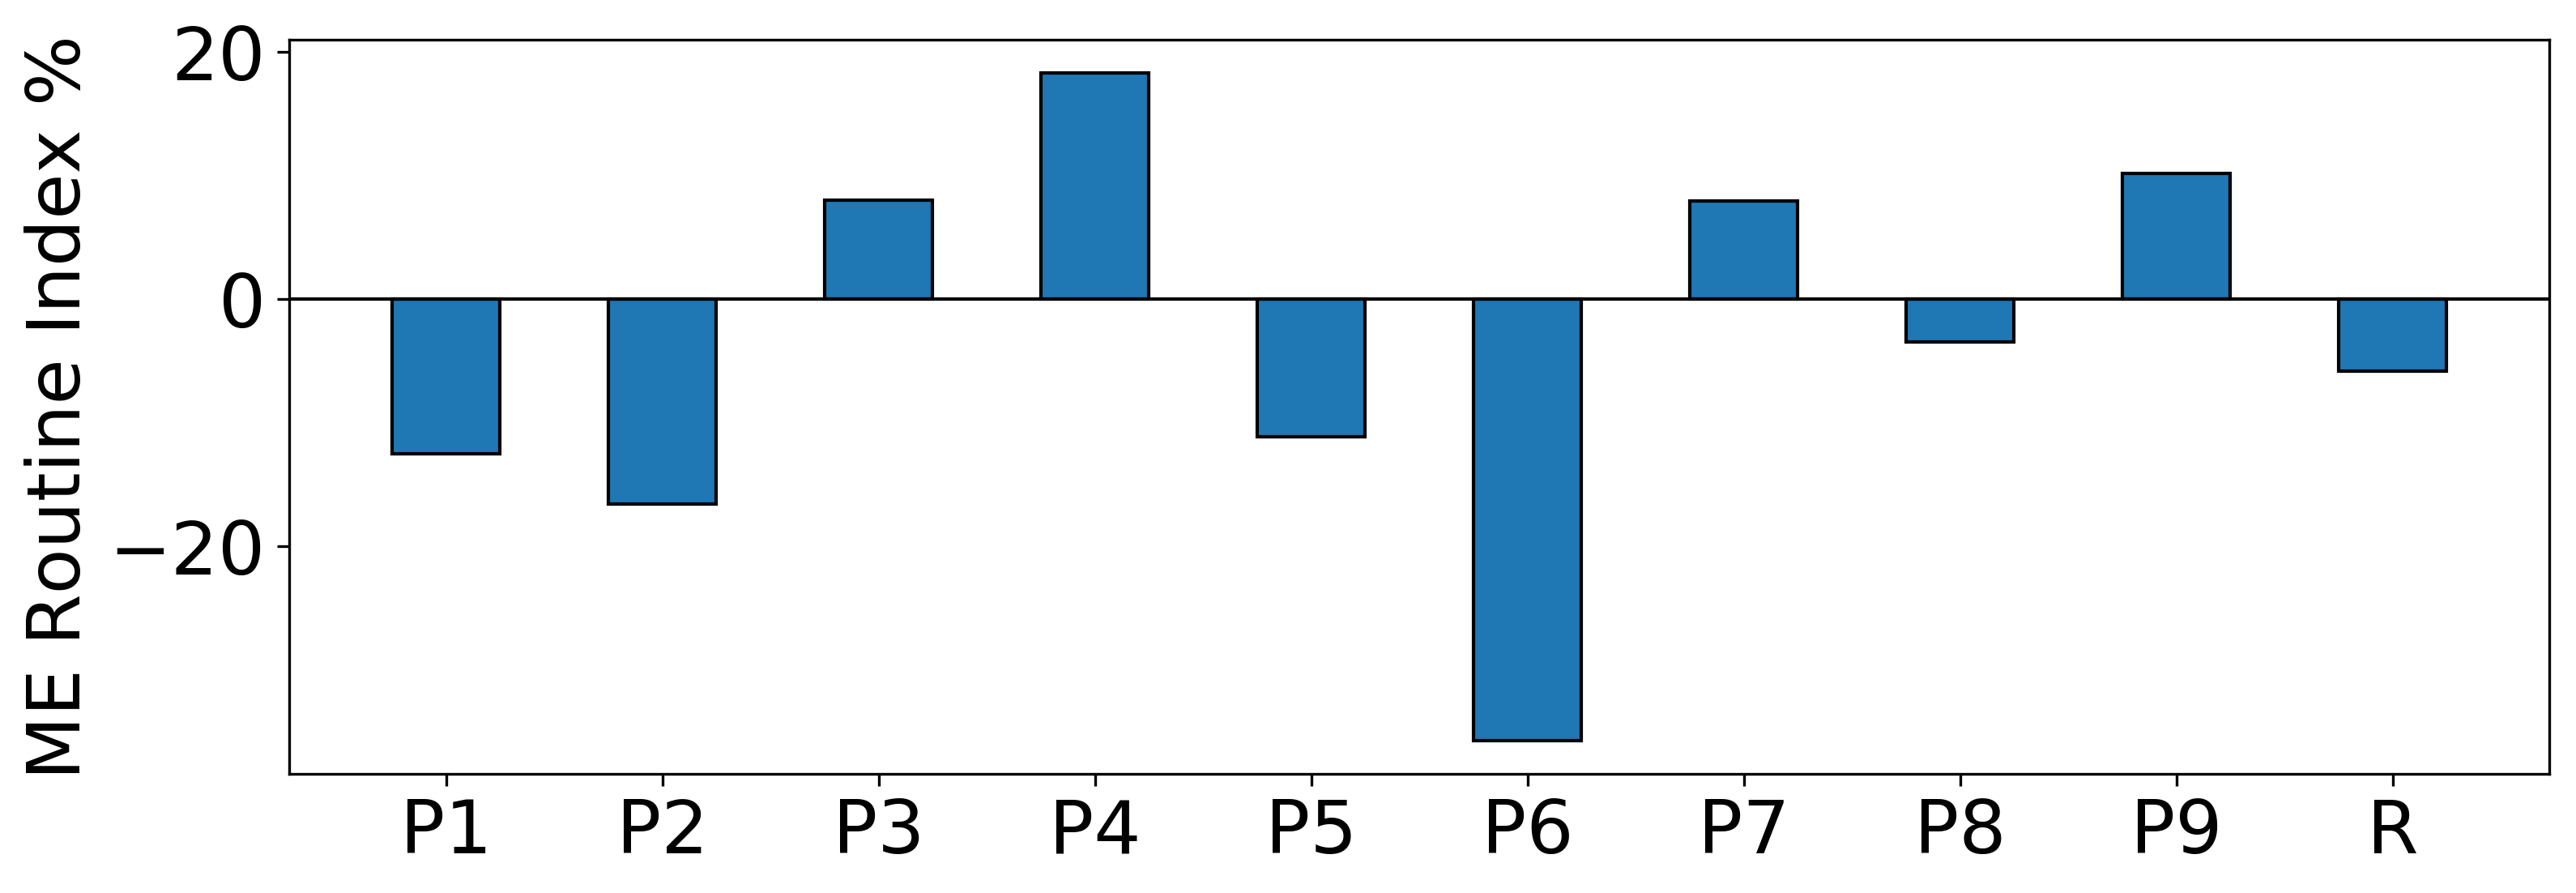
\includegraphics[width=\textwidth]{images/study/me_routine.png}
    \caption{The mean error for each participant for each of the three features. A negative mean error means the computed feature undershoots, and a positive error means it overshoots}
    \label{fig:plot-mean-error}
\end{figure}




\section{Improvements and Future Work}
The application development process led to many of the improvements of the package API reflected in Chapter \ref{chapter:04} and \ref{chapter:05}, mostly pertaining to moving processing inside the package rather than outside, and giving the application developer more restricted access. However, a couple of issues still remain both in terms of the API and the feature accuracy.

\subsection{Feature Accuracy}
The field study resulted in a dataset of 2.5M data points which means there would have been an opportunity for tuning the parameters if time allowed. Parameter tuning would increase the accuracy of the features produced by the algorithms and thereby increase its usefulness. Some features vary greatly in their accuracy from participant to participant and it is unknown whether that is down to the commitment of the participants and how diligent they were in tracking their location, as well as their answering, or whether the algorithms simply do not consider certain commonly occurring edge cases. Not all of the days are annotated as previously discussed, far from it, however a researcher can go by the days manually one by one for each participant and label certain of the features such as places visited, and to some extent the Home Stay and Routine Index, although the latter two would require a great effort of fine-combing the the data-sets. If feature-labeling was performed then it would simply be an optimization task where the optimal parameters for Stops and Moves are the parameters and the error of accuracy the objective to minimize. 

\subsection{Forced Daily Computation}
Currently the implementation throws away Location Samples from previous days when computing the MobilityContext for today. This approach assumes that any data left from a previous date has been transformed into Stops and Moves, and therefore no longer is needed. However does not consider the case where a large part of the stored Location Samples have not been used, due to no computation having taken place. In some cases whole days of Location Samples may end up being thrown away without Stops and Moves being computed from this data. The current way to avoid this is to compute features every day, making sure at least one computation takes place late in the evening such that minimal data is lost. Another way around it currently is to override the date, if is known that computation did not take place for a given date. This 'latest date of computation' can be kept track of by the programmer, but goes back to the problem of managing complexity. Ideally this is done by the package itself, and can be solved the following way:
When Location Samples are loaded, group them by date, and compute Stops and Moves for each of these dates. Save the Stops and Moves, and then throw away the samples from these previous dates. out.

\subsection{Asynchronous Computation}
The asynchronous computation is cumbersome to set up and takes over 30 lines of code to perform. This should ideally be moved inside the package in the next iteration. Another improvement to make is not relying on lazy evaluation, as discussed in Chapter \ref{chapter:05}. In the current version, only the intermediate Features will be computed in the background thread, whereas all the derived features contained in the MobilityContext object returned by the asynchronous computation will not yet have been computed upon returning from the background thread. This is due to \textit{lazy evaluation}, which ensures that the features are not unnecessarily computed in advance, and only computed once they are requested. This could potentially mean freezing the UI thread, since the features computed via lazy evaluation will be computed once the Mobility Context object is inside the main thread. The fix for this is to evaluate all features in the constructor of the Mobility Context class, which will imply longer guaranteed computation time for creating a Mobility Context object but will also guarantee that all features have been pre-computed in the background thread and will not block the UI thread. 

\subsection{Example Application}
The Pub package manager requires packages to have an example application to demonstrate its usage. Since the study application used an old version of the package API and does not display data, it should probably not be used further. Instead, the old version of the study app displayed in \ref{fig:app-features-screen} is a good candidate for an example app since it presents the calculated features to the user and can be implemented in a dynamic fashion were features are constantly recomputed and updated.

\subsection{CAMS Integration and Maintenance}
The package fits into the \textit{CARP Mobile Sensing Framework} as previously mentioned and will therefore continue to exist beyond this thesis. An integration into CAMS was not made as part of this thesis due to time constraints and the scope of the thesis. This integration will be made in the weeks following the thesis such that it may be easily implemented into existing CACHET projects such as MUBS by Rohani \cite{mubs-rohani}. For the foreseeable future it will be maintained by the Author, who will continue his employment at CACHET as a research assistant. 
\section{Package Maintenance}


\section{Future Work}
\subsection{Maintenance}
A big point of interest
It will be a real package alongside the other CARP packages
Will be maintained by CACHET, maybe me?

\subsection{Integrations}
Integrating this into apps people already\\
Give concrete recommendations, ex Rohani MUBS\\   



\section{User Prompting in Real-Time}
When should the user be given recommendations\\
Trigger can be time interval or threshold for a feature, i.e. if homestay greater than 0.5 prompt the user to leave the house\\
Recommendations from depression database (Rohani, 300 items, not part of this thesis)\\

Calculate routine index from week to week rather than day to day. Currently we assume that all days ideally look identical, which for most people will not be the case. For many people the weekends differ quite a lot from their every day, and naturally the routine index will therefore be lower during the weekend, and weekend days will tend to 'wash out' the routine index calculation. 
\chapter{Conclusion}
\label{chapter:08}
Novel routine index
Real time feature calculation design
% \blinddocument

\appendix
%!TEX root = ../Thesis.tex

\chapter{Nomenclature}
\begin{acronym}[TDMA]
\acro{CACHET}{Copenhagen Center for Health Technology} 
\acro{MDD}{Major Depressive Disorder} 
\acro{BA}{Behavioural Activation} 
\end{acronym}

\textbf{Major Depressive Disorder (MDD)}\\
Also known simply as depression, is a mental disorder characterized by low mood, low self-esteem, loss of interest in normally enjoyable activities, low energy, and pain without a clear cause.\\

\textbf{Behavioural Activation (BA)}\\
A therapeutic intervention that is often used to treat MDD. BA treatment focuses on keeping depression at bay through activities which produce positive reinforcement for the patient. BA is highly customizable and is a very personal treatment plan.\\

\textbf{Mobility}\\
How a person changes location over time.\\

\textbf{Mobility Feature}\\
A number which describes one of the ways in which a person changes location over time. Many features will paint a more complete picture of the mobility patterns than fewer features.\\

\textbf{Pre-processing}\\
TODO.\\




%!TEX root = ../Thesis.tex
\chapter{Questionnaires}
\label{appendix:questionnaires}
\subsection{PHQ-9 (Patient Health Questionnaire)}
Patented by Pfizer

The PHQ-9 questionnaire contains 9 questions pertaining to the mental state of the patient \footnote{\url{https://patient.info/doctor/patient-health-questionnaire-phq-9}}. Each question asks ‘Over the last two weeks, how often have you been bothered by any of the following problems?’ with the questions being the following: \\

\textbf{Q1:} Little interest or pleasure in doing things? \\

\textbf{Q2:} Feeling down, depressed, or hopeless? \\

\textbf{Q3:} Trouble falling or staying asleep, or sleeping too much? \\

\textbf{Q4:} Feeling tired or having little energy? \\

\textbf{Q5:} Poor appetite or overeating? \\

\textbf{Q6:} Feeling bad about yourself, or that you are a failure, or have let yourself or your family down? \\

\textbf{Q7:} Trouble concentrating on things, such as reading the newspaper or watching television? \\

\textbf{Q8:} Moving or speaking so slowly that other people could have noticed. Or the opposite – being so fidgety or restless that you have been moving around a lot more than usual? \\

\textbf{Q9:} Thoughts that you would be better off dead, or of hurting yourself in some way? \\

Each question can be answered with the following 4 possibilities, each giving a number of points indicated in brackets:

\begin{itemize}
\item Not at all (0 points)
\item Several days (1 point)
\item More than half the days (2 points)
\item Nearly every day (3 points)
\end{itemize}

At the end of the survey, the points are summed up and the patient is categorized into one of 5 categories based on the number of points acquired:

\begin{itemize}
\item Less than 5 (no depression)
\item 5-9 (mild depression)
\item 10-14 (moderate depression)
\item 15-10 (moderate/severe depression)
\item Greater than 20 (severe depression)
\end{itemize}


\subsection{EMA (Ecological Momentary Assessment)}
The EMA Questionnaire contains six short questions each targeting a common mental state strongly related to depression, each for which the user has to give a self-perceiving rating from 1 (none) to 7 (extreme):

\begin{itemize}
\item Negative Affect
\item Hopelessness
\item Anhedonia (loss of interest)
\item Fatigue/Energy
\item Loneliness
\item Positive Affect
\end{itemize}
\chapter{Package Documentation}
\section{Structure}
\label{appendix:package}
The package contains two main directories and three metadata files as depicted in Figure \ref{fig:package-structure}. The first directory is the source code directory, \textit{lib}, containing the domain model, and algorithms for computing MobilityContexts. The second directory is the \textit{test} directory containing unit tests which aid in the process of validating the algorithms. The metadata files are the \textit{CHANGELOG.md} which contains a list of changes made to the package such that an application programmer can keep track of changes to the API. 

\begin{figure}
    \centering
    \begin{verbatim}
        mobility_features
        ├── lib/
        │   ├── mobility_context.dart
        │   ├── mobility_domain.dart
        │   ├── mobility_features.dart
        │   ├── mobility_functions.dart
        │   ├── mobility_intermediate.dart
        │   └── mobility_serializer.dart
        ├── test/
        │   ├── data/
        │   ├── mobility_features_test.dart
        │   └── test_utils.dart
        ├── CHANGELOG.md
        ├── pubspec.yaml
        ├── README.md
    \end{verbatim}
    \caption{The file structure of the Mobility Features Flutter Package}
    \label{fig:package-structure}
\end{figure}

The \textit{pubspec.yaml} contains the package specification including the package name, a description, version, homepage, and a list of dependencies. The dependencies are other packages on which the package depends, as in this case, the Mobility Features Package depends on the \verb|simple_cluster|, \verb|stats| and \verb|path_provider| packages each with a specific version number. The package itself also has such a version number that allows an application developer to import a specific version of the package, for example, if they built their application around a previous release, they may wish to continue depending on that specific release rather than upgrading to the newest version.

\begin{figure}
    \centering
    \begin{minted}{yaml}
        name: mobility_features
        description: Real-time mobility feature calculation
        version: 1.1.5
        homepage: https://github.com/cph-cachet/flutter-plugins/
        
        environment:
          sdk: ">=2.7.0 <3.0.0"
        
        dependencies:
          flutter:
            sdk: flutter
          simple_cluster: ^0.2.0
          stats: ^0.2.0+3
          path_provider: ^1.6.10
        
        dev_dependencies:
          flutter_test:
            sdk: flutter
    \end{minted}
    \caption{The pubspec.yaml file for the Mobility Features Package}
    \label{fig:pubspec}
\end{figure}

Lastly, the README.md file contains instructions for using the package including code snippets and use case examples. 

\section{Publishing}
Distributing a Flutter package is done via the Dart Package Manager, Pub. Pub is essentially a git repository of a package including all versions of that package. When publishing a package the contents of the README file are converted to HTML and are what the user is initially presented with. The README should, therefore, give a brief overview and description of the package, in addition to instructions. Figure \ref{fig:pub-package} shows the latest version of the package hosted at \url{https://pub.dev/packages/mobility_features}.

\begin{figure}
    \centering
    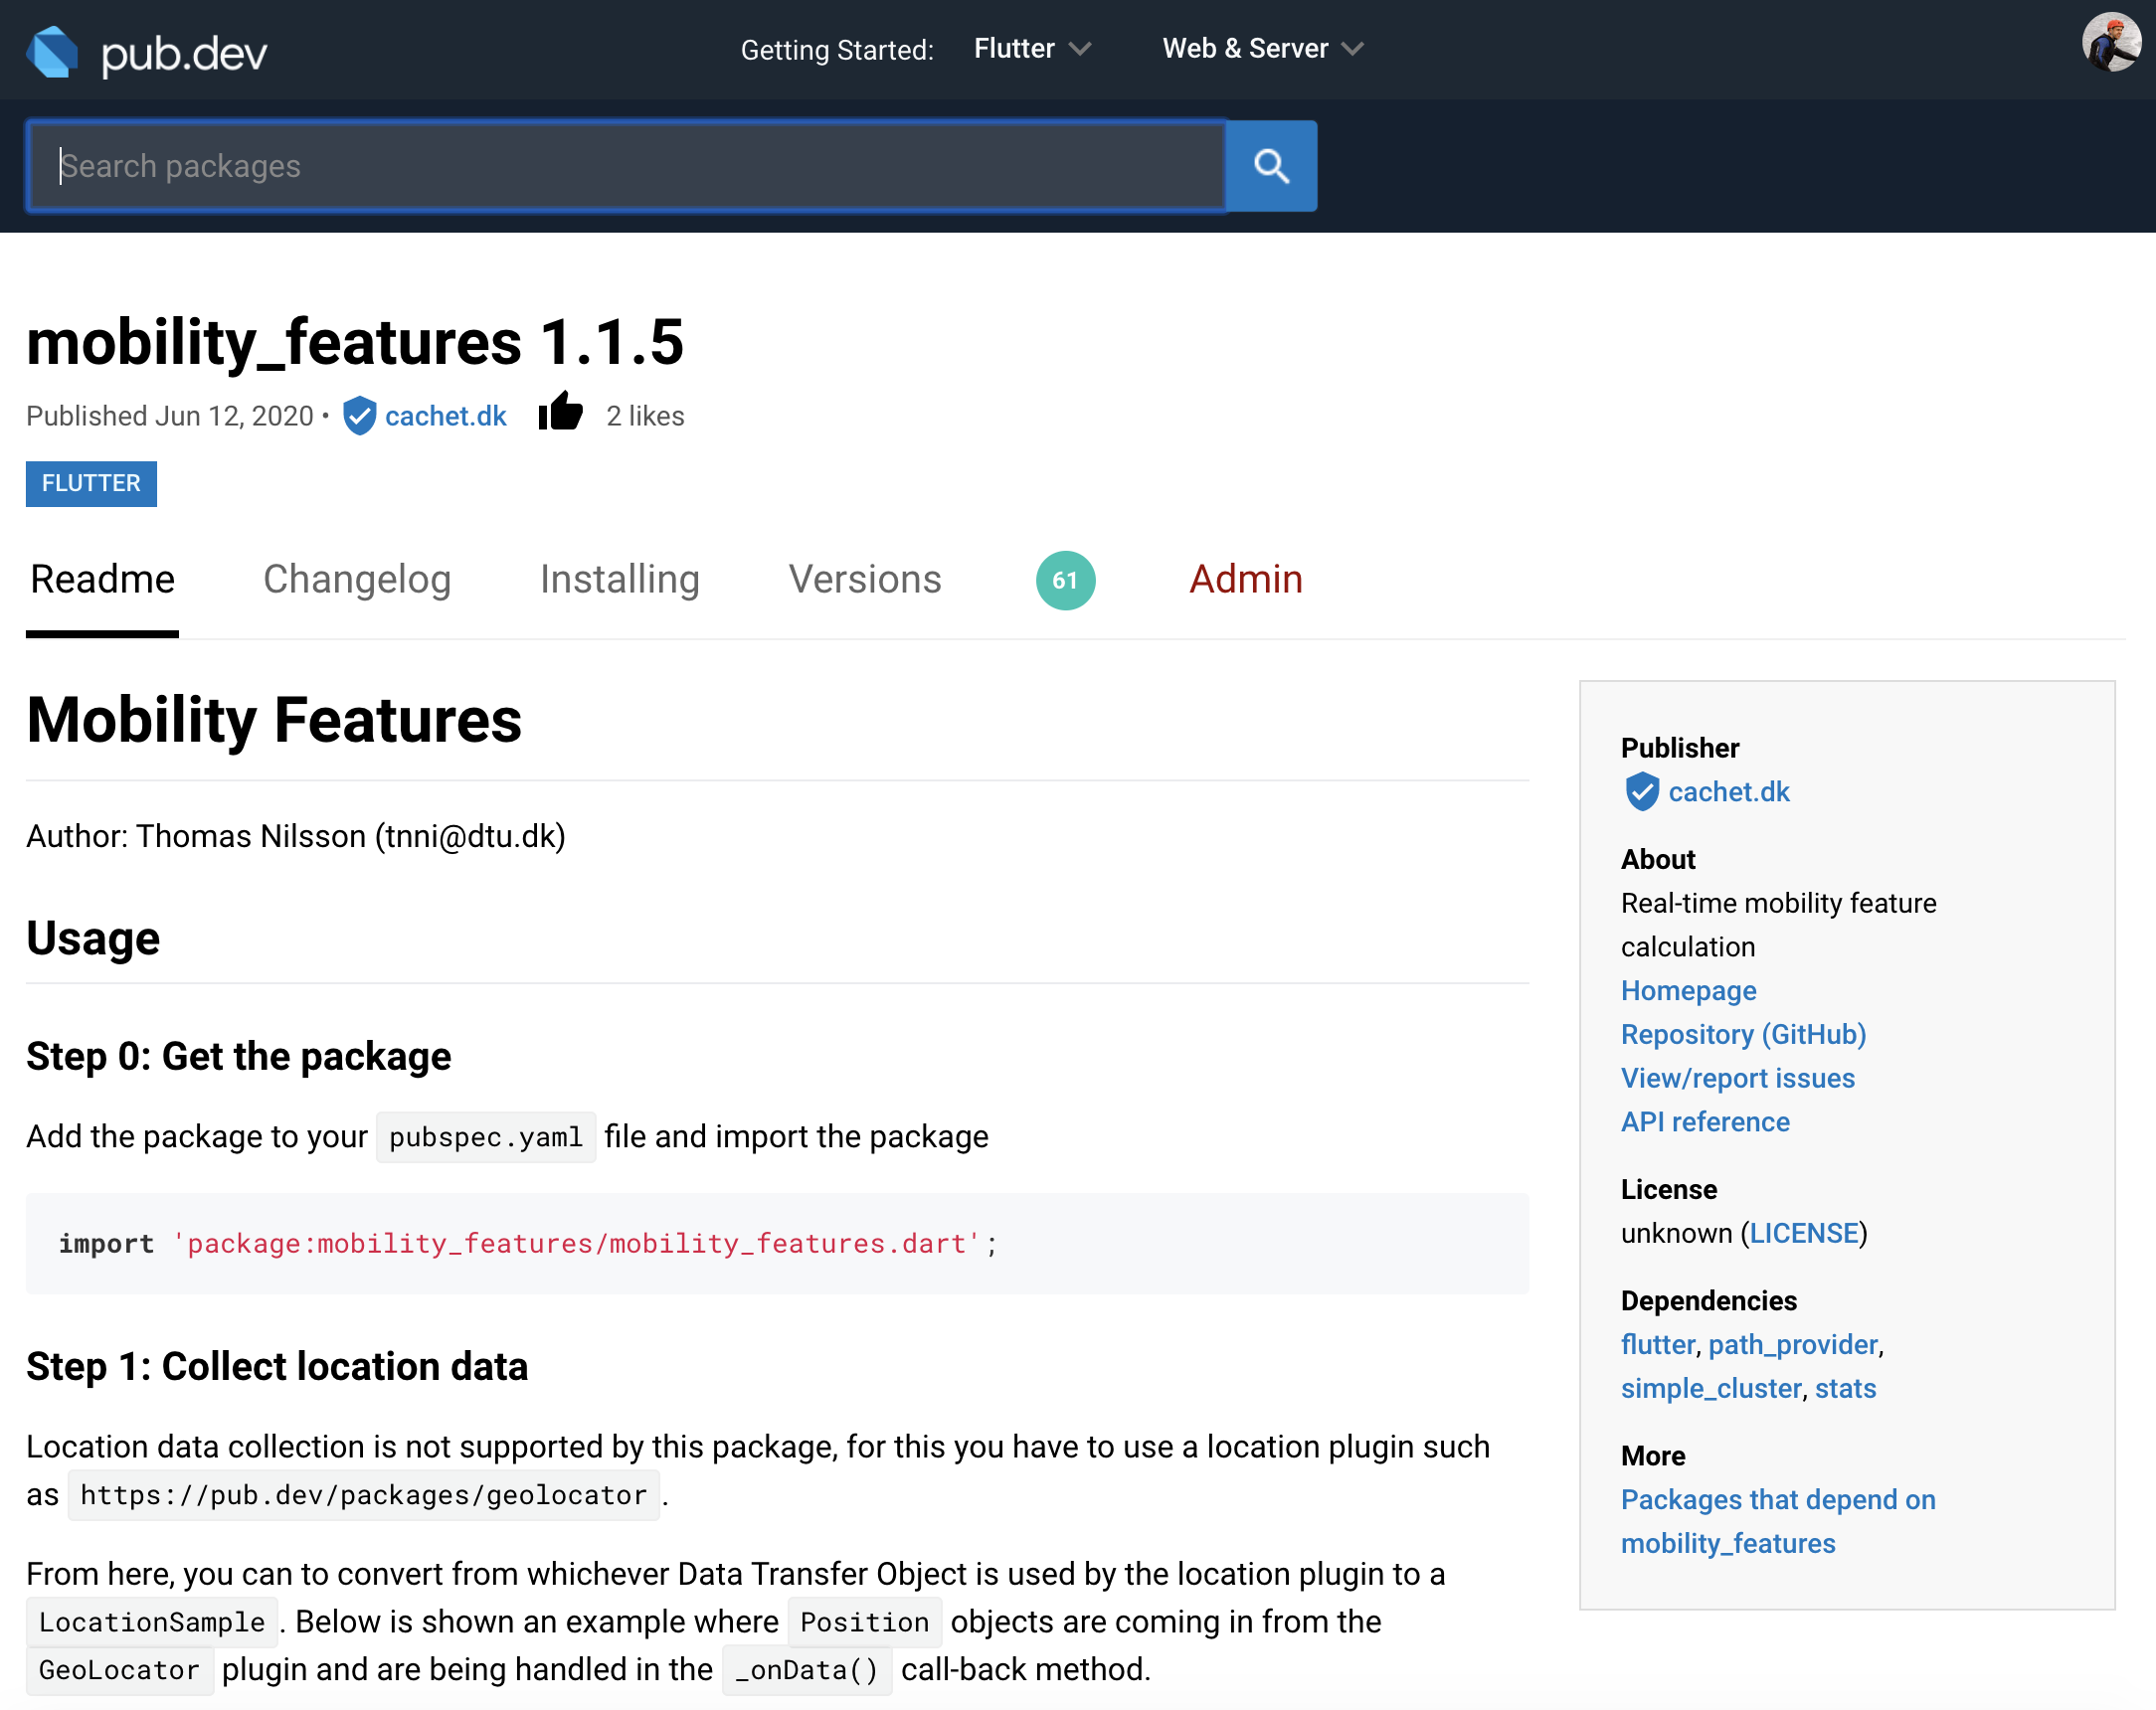
\includegraphics[width=\textwidth]{images/pub.png}
    \caption{The page hosting the Mobility Features Package on www.pub.dev}
    \label{fig:pub-package}
\end{figure}

Publishing automatically generate API documentation by using comments in the code. Normally, comments are made with 2 forward slashes (\textit{//}), but comments made with three forward slashes (\textit{///}) mark the code-block following it with API documentation, i.e. the contents of the comment. 

\begin{figure}
    \centering
    \begin{minted}{dart}
    /// A [LocationSample] holds a 2D [GeoPosition] spatial data point
    /// as well as a [DateTime] value s.t. it may be temporally ordered
    class LocationSample implements _Serializable, _Geospatial {...}
    \end{minted}
    \caption{The API comments for the source code of the Location Sample class}
    \label{fig:api-comments}
\end{figure}

\begin{figure}
    \centering
    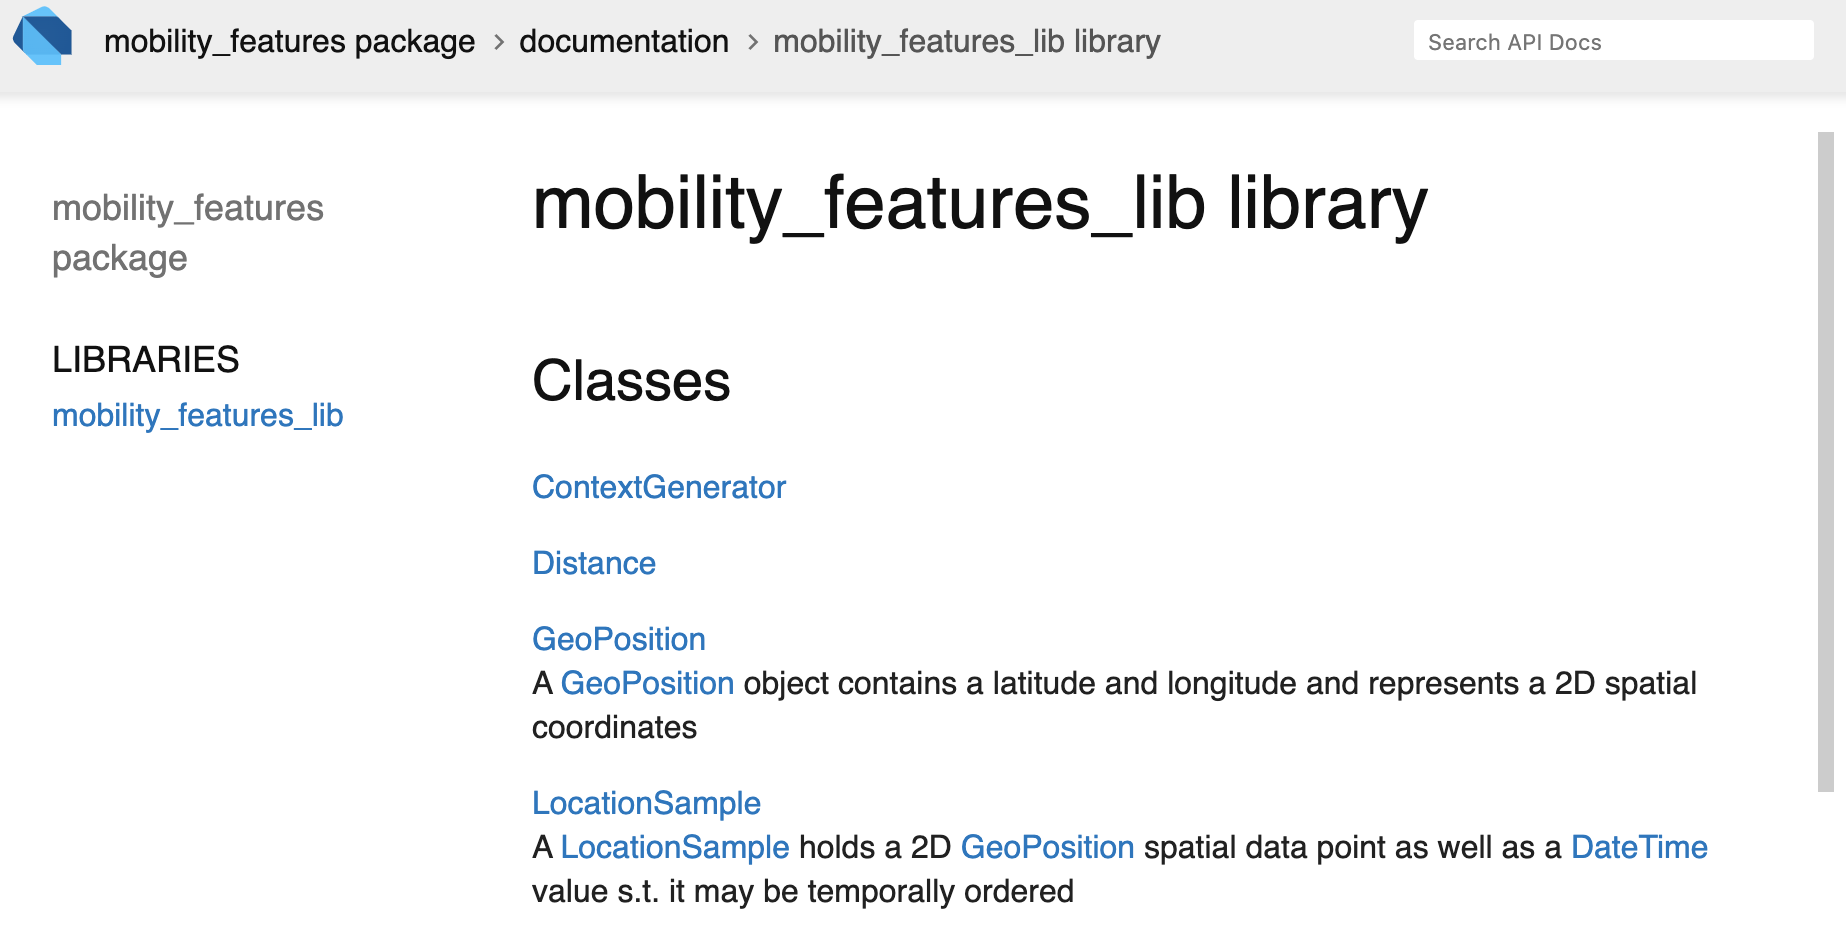
\includegraphics[width=\textwidth]{images/docs.png}
    \caption{The auto generated documentation for the package, hosted on pub.dev, including the code snippet in Figure \ref{fig:api-comments} for the Location Sample class}
    \label{fig:api-docs}
\end{figure}



\chapter{Python Demo}
\label{appendix:python-demo}
The following pages contain the Python implementation of the offline feature algorithms which is run on a synthetic dataset. This was used in the development process since prototyping in Python is much faster than in Dart.

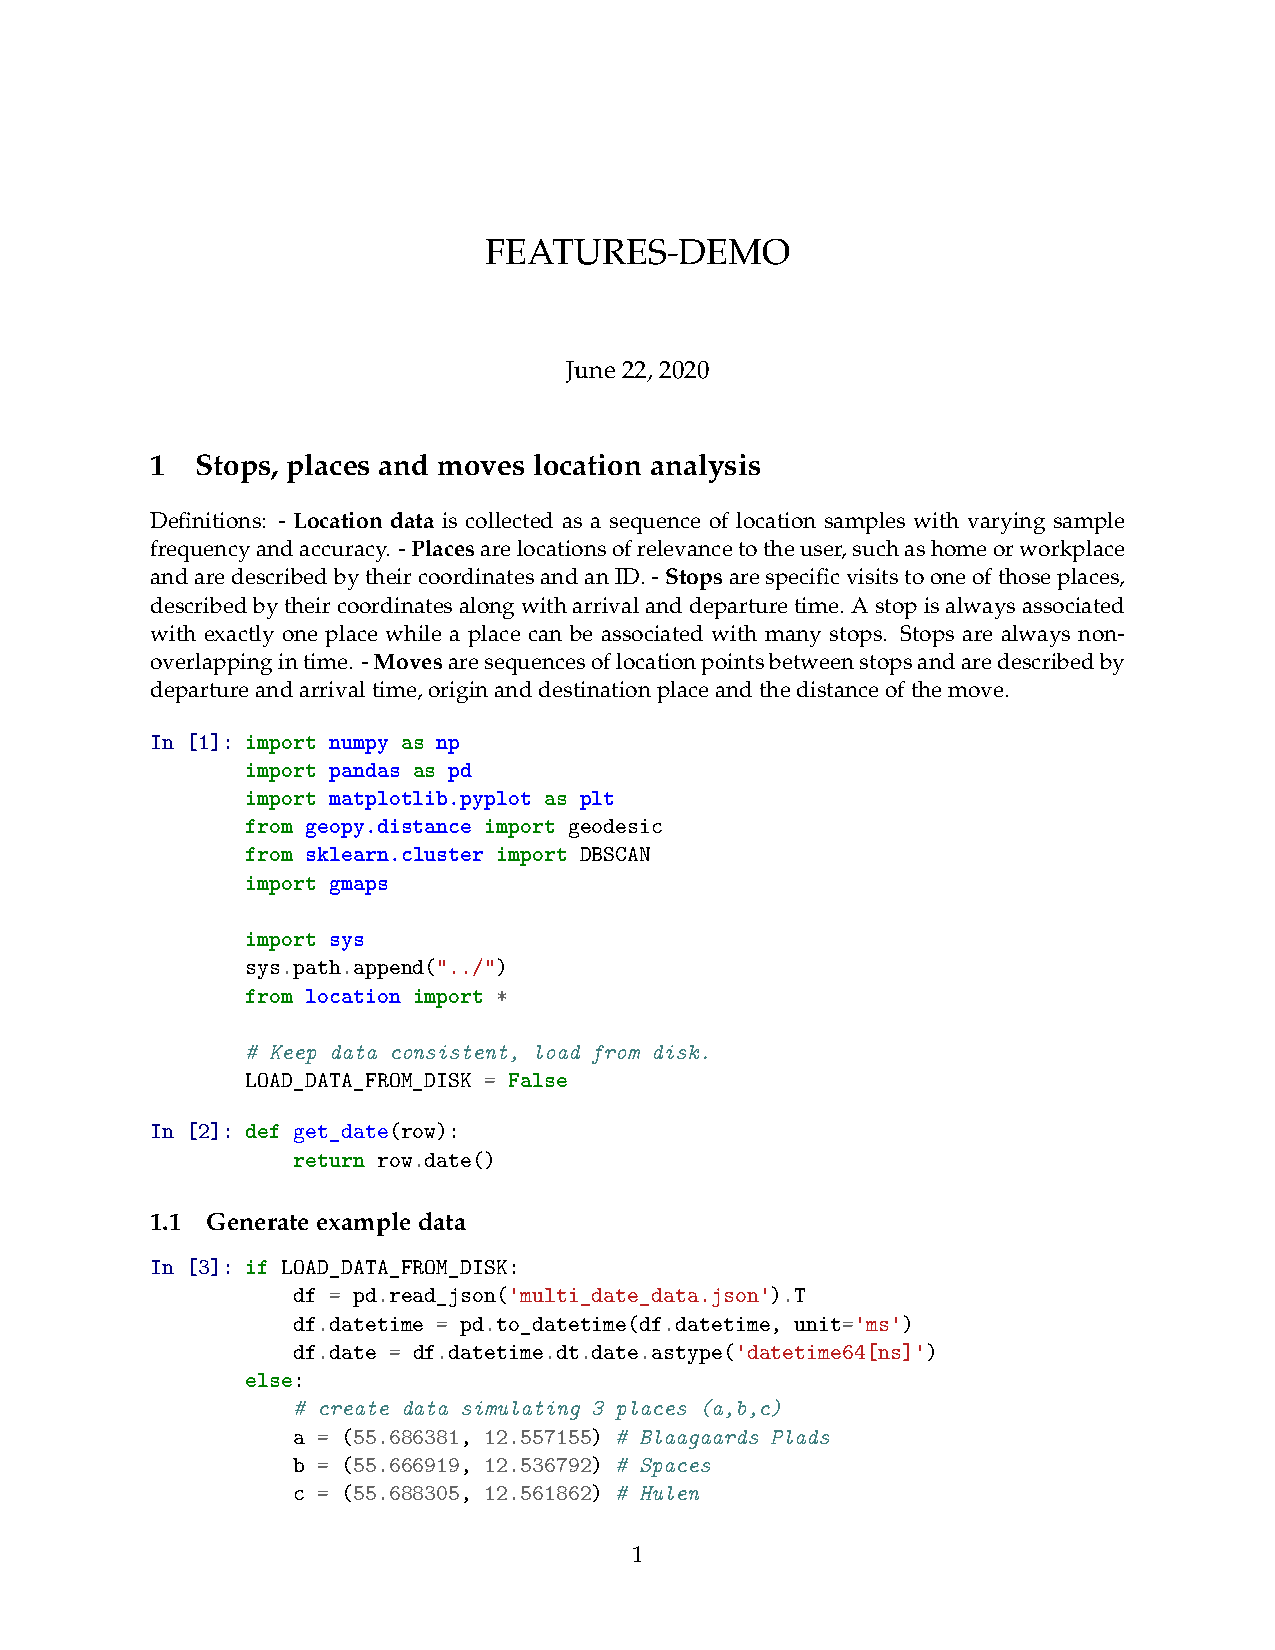
\includepdf[pages=-,pagecommand={},width=\textwidth]{appendices/FEATURES-DEMO.pdf}
\chapter{Source Code}
\label{appendix:source-code}
\subsection{Storing and Loading Data}
The storing and loading of data, which includes Location Samples, Stops, and Moves happen through the \textit{MobilitySerializer} class. This class allows classes that implement the Serializable interface to be serialized and de-serialized. Just like the GeoSpatial interface, the Serializable interface is also implemented as a private abstract class only used internally in the package library. The interface contains a method for serializing a class to JSON, named \verb|toJson()| which takes no parameters and produces a HashMap of Strings to the dynamic, the dynamic type meaning any type. This is the Dart equivalent of a JSON object. Another method the interface forces other classes to implement is the deserialization method \verb|fromJson(json)| which takes a JSON object as a parameter and creates a runtime object of the given type, from the JSON object. The implementation of this method is left to the individual classes implementing the interface which is done by extracting data from the JSON object.

\begin{minted}{dart}
    abstract class _Serializable {
      Map<String, dynamic> _toJson();
    
      _Serializable._fromJson(Map<String, dynamic> json);
    }
\end{minted}

The MobilitySerializer class is a generic which allows the type \verb|E| to be specified later, with \verb|E| referring to either a Location Sample, Stop or Move which all implement the Serializable interface. The MobilitySerializer is constructed using a reference to a File object. The File object is used for storing the data of the given type i.e. Location Samples are stored one file, Stops in another, and Moves in a third.

\begin{minted}{dart}
    class MobilitySerializer<E> {
      File file;
      
      MobilitySerializer._(this.file) {
        bool exists = file.existsSync();
        if (!exists) {
          flush();
        }
      }
      
      Future<void> flush() async =>
          await file.writeAsString('', mode: FileMode.write);
    ...
    }
\end{minted}

When initialized, it is checked whether or not the specified file exists, and if not the \verb|flush| method is called, which simply writes an empty string to the file, overriding any content, which has the effect of creating the file, should it not already exist. A concrete example of instantiated the MobilitySerializer for Stops is shown below, where \textit{stops.json} refers to the file in which Stops should be stored.

\begin{minted}{dart}
    MobilitySerializer<Stop> stopSerializer =
            MobilitySerializer<Stop>._(await _file('stops.json'));
\end{minted}

For storing data the \verb|save| method is used which takes in a list of objects which all implement the Serializable interface. Each element in the list is serialized via its \verb|toJson| method and concatenated into one big string separated by a delimiter token, and this string is then written to the specific file of the MobilitySerializer object.

\begin{minted}{dart}
    Future<void> save(List<_Serializable> elements) async {
      String jsonString = "";
      for (_Serializable e in elements) {
        jsonString += json.encode(e._toJson()) + delimiter;
      }
      await file.writeAsString(jsonString, 
        mode: FileMode.writeOnlyAppend);
    }
\end{minted}

Loading works in the reverse order, where the contents of the specified file are loaded into a string, the string is then split into elements using the delimiter token and each of these elements is de-serialized using the \verb|fromJson| method.  For deciding which type to de-serialize the elements into, a switch statement is used that checks the type of \verb|E| which is specified when the MobilitySerializer object is instantiated.

\begin{minted}{dart}
    Future<List<_Serializable>> load() async {
        String content = await file.readAsString();
    
        List<String> lines = content.split(delimiter);
    
        Iterable<Map<String, dynamic>> jsonObjs = lines
            .sublist(0, lines.length - 1)
            .map((e) => json.decode(e))
            .map((e) => Map<String, dynamic>.from(e));
    
        switch (E) {
          case Move:
            return jsonObjs.map((x) => 
                Move._fromJson(x)).toList();
          
          case Stop:
            return jsonObjs.map((x) => 
                Stop._fromJson(x)).toList();
          
          default:
            return jsonObjs.map((x) => 
                LocationSample._fromJson(x)).toList();
        }
    }
\end{minted}

Ideally, the switch statement could have been replaced by the following one-liner:
\begin{minted}{dart}
    return jsonObjs.map((x) => E.fromJson(x)).toList();
\end{minted}

However, this relies on the language feature called reflection \footnote{\url{https://www.javaworld.com/article/2075801/reflection-vs--code-generation.html}} which allows the compiler to infer the type of \verb|E| at compile-time. However, Dart does not support \textit{reflection} which makes this impossible.


\subsubsection{Accessing the File System}
For storing collected location data the MobilitySerializer for Location Samples can be retrieved through this class, with a getter method. 
);
\begin{minted}{dart}
static Future<MobilitySerializer<LocationSample>>
      get locationSampleSerializer async =>
          MobilitySerializer<LocationSample>._(await _file(LOCATION_SAMPLES)
\end{minted}

Internally this class has a method for creating a file system reference, which relies on the platform the application is running on. For mobile apps, the file system must be accessed through the \verb|path_provider| package with the \verb|getApplicationDocumentsDirectory()| method. If the application is run on the desktop, such as when unit testing the file system can be accessed by specifying a file name directly. This is a textbook example of hiding complexity from the application programmer.

\begin{figure}
    \centering
    \begin{minted}{dart}
    static Future<File> _file(String type) async {
      bool isMobile = Platform.isAndroid || Platform.isIOS;
    
      String path;
      if (isMobile) {
        path = (await getApplicationDocumentsDirectory()).path;
      } else {
        path = 'test/data';
      }
      return new File('$path/$type.json');
    }
    \end{minted}
    \caption{Lazy evaluation of a feature}
    \label{fig:lazy-evaluation}
\end{figure}


\chapter{Unit Testing}
\label{appendix:unit-testing}
Unit testing \footnote{\url{https://martinfowler.com/bliki/UnitTest.html}}, in which small parts of the source code are tested played a significant role in the latter part of the development process. It was prioritized to make a working demo application in order to conduct a study and while unit tests can speed up certain parts of the debugging process, it was still faster to 'hack something together'. The only testing done prior to the study was regarding serialization and making sure the feature computation producing meaningful results, i.e. they were manually verified. The traditional way of using unit testing is through Test-Driven Development developed by Kent Beck \cite{beck-tdd} in which the tests are written first, and the corresponding source code which should pass the test is written afterward. The package went through many smaller iterations, in which the data flow was moved around, and unit testing made discovering bugs much easier by enabling one to constantly verify that the source code produced the desired results every time changes were made. As the package went through multiple iterations, each iteration either added or removed functionality or changed the existing functionality slightly which meant new unit tests were often written to cover the functionality. In the end, some the functionality was pruned and therefore some of the tests were also superfluous or had a large amount of overlap between them and were therefore also consolidated. 

\subsection{Limitations of Unit Testing}
There were a few shortcomings of unit testing encountered, which largely came down to the inability to compare objects before and after serialization. This stems from objects having a hash code, i.e. a unique fingerprint which is not stored when serializing. The fingerprint is used to compare objects while in memory, and since the fingerprint is lost the problem arises. For this to be resolved, a better testing method needs to be implemented in terms of comparing objects. This can be done by implementing a function that breaks down each object, be it a Stop, or MobilityContext, into the most atomic values, i.e. latitude, longitude, time-stamp, etc, which can be compared without a hash code. For testing the algorithms, small synthetic datasets were created in order to test very rudimentary cases. It was harder to construct very large synthetic datasets in order to test more realistic, noisy datasets and discover edge cases. In the future, more elaborate unit tests should be written, especially for the clustering algorithms, since the ground truth, i.e. cluster centroids and points belonging to clusters can be calculated by hand. Another possibility that was partly explored was using a real-world dataset that the author gathered tracking himself however to verify the algorithms on this dataset it would need to manually label which was not done. The large real-world dataset was however used to verify that the algorithms produced meaningful results and that the computation did not throw any errors. Lastly, the current state of the API gives the public access to certain methods which are not supposed to have public access. The reason for this is that they need to be part of the unit tests, concretely it is the MobilitySerializer methods \textit{flush} and \textit{save}. These methods are not intended to be used by the user since the flush method deletes all contents of the corresponding file. The load method does not pose a threat to the usability, but is unnecessary clutter, and should only be used internally by the package. 

\subsection{Example Unit Tests}
In this subsection selected unit tests will be exemplified.

\subsubsection*{Location Sample Serialization}
This test is the simplest unit test in the collection in which the storing- and loading functionality of the MobilitySerializer is displayed. A small, synthetic is created consisting of three Location Samples, which is first stored via the save() method, and next the load() method is called. To check whether or not the store and load were successful, the lengths of the original dataset and the loaded dataset are compared. 

\begin{figure}
    \centering
    \begin{minted}{dart}
    test('Serialize and load three location samples', () async {
      MobilitySerializer<LocationSample> serializer =
          await ContextGenerator.locationSampleSerializer;

      LocationSample x =
          LocationSample(GeoPosition(123.456, 123.456), DateTime(2020, 01, 01));


      List<LocationSample> dataset = [x, x, x];

      await serializer.flush();
      await serializer.save(dataset);
      List loaded = await serializer.load();
      expect(loaded.length, dataset.length);
    });
    \end{minted}
    \caption{A unit testing demonstrating storing and loading a small, synthetic dataset}
    \label{fig:my_label}
\end{figure}

\subsubsection*{Test: Single Stop}
This test is a step up in complexity in terms of what is tested. A dataset is constructed that simulates a user staying at a single location from 00:00 to 17:00. This should result in a single stop and place being found, no moves, and a homestay value of 1.0 (i.e. 100 percent). The data is first serialized and a Mobility Context is computed afterward from which the features are extracted.

\begin{figure}
    \centering
    \begin{minted}{dart}
    test('Features: Single Stop', () async {
      Duration timeTracked = Duration(hours: 17);

      List<LocationSample> dataset = [
        // home from 00 to 17
        LocationSample(loc0, jan01),
        LocationSample(loc0, jan01.add(timeTracked)),
      ];

      MobilitySerializer<LocationSample> serializer =
          await ContextGenerator.locationSampleSerializer;

      serializer.flush();
      await serializer.save(dataset);

      MobilityContext context = 
        await ContextGenerator.generate(today: jan01);
      expect(context.homeStay, 1.0);
      expect(context.stops.length, 1);
      expect(context.moves.length, 0);
      expect(context.places.length, 1);
    });
    \end{minted}
    \caption{Unit test for a single Stop}
    \label{fig:test-single-stop}
\end{figure}

\subsubsection*{Test: Multiple Days with Routine Index}
This test works similarly to the previous one but has the dataset spread over two different locations. The same dataset is repeated for 5 days, where the number of Stops, Moves, and Places is evaluated each day, in addition to the Home Stay and Routine Index feature. Concretely, the places visited are the same each day, at the same hours of the day meaning the Routine Index is 1.0 except for the first day since the Routine Index requires at least one historical day for comparison. The user stays at one place from 00:00 to 06:00 making it the home cluster, and another place from 08:00 to 09:00. This means the Home Stay should be equal to $\frac{6}{9}$, or 66.67 percent. 


\begin{figure}
    \centering
    \begin{minted}{dart}
    test('Features: Multiple days, multiple locations', () async {
      MobilitySerializer<LocationSample> serializer =
          await ContextGenerator.locationSampleSerializer;

      /// Clean file every time test is run
      serializer.flush();

      for (int i = 0; i < 5; i++) {
        DateTime date = jan01.add(Duration(days: i));

        /// Todays data
        List<LocationSample> locationSamples = [
          // 5 hours spent at home
          LocationSample(loc0, date.add(Duration(hours: 0, minutes: 0))),
          LocationSample(loc0, date.add(Duration(hours: 6, minutes: 0))),

          LocationSample(loc1, date.add(Duration(hours: 8, minutes: 0))),
          LocationSample(loc1, date.add(Duration(hours: 9, minutes: 0))),
        ];

        await serializer.save(locationSamples);

        /// Calculate and save context
        MobilityContext context = await ContextGenerator.generate(
            usePriorContexts: true, today: date);

        double routineIndex = context.routineIndex;
        double homeStay = context.homeStay;

        expect(context.stops.length, 2);
        expect(context.places.length, 2);
        expect(context.moves.length, 1);

        expect(homeStay, 6 / 9);

        // The first day the routine index should be -1,
        // otherwise 1 since the days are exactly the same
        if (i == 0) {
          expect(routineIndex, -1);
        } else {
          expect(routineIndex, 1);
        }
      }
    });
    \end{minted}
    \caption{Unit test for a single Stop}
    \label{fig:test-single-stop}
\end{figure}
\chapter{Installation Manual}
\label{appendix:installation}

The following pages contains the instruction manual the participants were sent out, in order for them to install the application. The application was distributed via TestFlight where each participant received an invitation via their Apple ID.

\includepdf[pages=-,pagecommand={},width=1.2\textwidth]{appendices/installation.pdf}


\chapter{Data Analysis - Extra Plots}
\label{appendix:data-analysis}
\section{Missing Data}

Figure \ref{fig:p8-gaps} shows the collected location data for participant P8 who had an older phone (iPhone 6s) which has limited memory and compute resources, which likely impacted how much data was tracked. The participant was very diligent in making sure the phone tracked at all times, yet substantial gaps still exist.

\begin{figure}
    \centering
    \includegraphics[width=\textwidth]{images/study/ec110976-0192-436d-b451-4f5dd97e71d8-gaps.png}
    \caption{An event plot for participant P8 who was diligent in making sure the phone was tracking, but had an older phone (iPhone 6s)}
    \label{fig:p8-gaps}
\end{figure}

\backmatter
\printbibliography

\end{document}
